\documentclass[openany,lang=cn,newtx,11pt,scheme=chinese,color=blue,mode=fancy,bibtex]{elegantbook}

\title{计算机网络知识点与例题解答}
\subtitle{第1--7章 · 依据课程PPT整理}
\author{}
\date{2026年11月16日}
\version{0.5}
\cover{ch01-internet.png}

\setcounter{tocdepth}{2}
\setcounter{secnumdepth}{2}
\usepackage{graphicx}
\usepackage{booktabs}
\usepackage{tabularx}
\usepackage{array}
\usepackage{enumitem}
\usepackage{float}
\graphicspath{{figure/source/}{notes/figure/source/}}
\newcount\annotationcounter
\makeatletter
\newcommand{\annotationarea}{\@ifnextchar[{\annotationarea@optional}{\annotationarea@required}}
\newcommand{\annotationarea@optional}[1][4]{\annotationarea@draw{#1}}
\newcommand{\annotationarea@required}[1]{\annotationarea@draw{#1}}
\newcommand{\annotationarea@draw}[1]{%
  \par\smallskip
  \noindent{\color{gray!65}\scriptsize 批注}\par
  {\color{gray!45}%
    \annotationcounter=#1\relax
    \loop\ifnum\annotationcounter>0
      \noindent\rule{\linewidth}{0.25pt}\par\vspace{0.6cm}%
      \advance\annotationcounter by -1
    \repeat
  }%
  \smallskip
}
\makeatother

% ElegantBook 的章标题仍可能继承 book 的 openright 状态；本笔记使用单面阅读版式。
\makeatletter\@openrightfalse\makeatother

\begin{document}
\raggedbottom
\fancyhead[R]{\color{structurecolor}\cnormal\leftmark}
\maketitle
\frontmatter
\tableofcontents
\mainmatter

\part{第1--7章知识点、例题与解答}
\chapter{计算机网络概述}

本章按课件的六部分展开：计算机网络基本概念、计算机网络结构、数据交换、计算机网络性能指标、计算机网络体系结构和计算机网络发展历史。课件第1.6节标注“略”；仍按课件保留其时间线，便于识别重要里程碑。本章中速率、设备和网络结构均以课件所列内容为准。

\section{计算机网络基本概念}

\subsection{通信系统与计算机网络}

计算机网络是通信技术与计算机技术结合的产物。课件给出的通信系统模型由\textbf{信源、发送设备、信道、接收设备、信宿}组成，并可能受到\textbf{噪声源}干扰：
\[
\text{信源}\longrightarrow\text{发送设备}\longrightarrow\text{信道}\longrightarrow\text{接收设备}\longrightarrow\text{信宿}.
\]
信源产生待传送的信息；发送设备把信息变成适合信道传送的信号；信道是信号经过的媒介；接收设备从信号中恢复信息；信宿是信息的最终使用方。噪声是对传输信号的干扰，可能使接收方得到错误信息。

\textbf{计算机网络}是\textbf{互连的、自治的计算机集合}。“互连”表示计算机之间能够借助通信链路交换数据；“自治”表示各计算机没有主从关系，每台计算机仍由自身控制。网络中的计算机通常称为\textbf{主机}或\textbf{端系统}。当距离远、计算机数量多时，不能给每两台计算机都单独铺设一条链路，因此需要交换设备组成交换网络。

\textbf{互联网（Internet）}是由大量互连的计算设备、通信链路和交换设备组成的网络。主机运行网络应用；光纤、铜缆、无线电和卫星等可作为通信链路；路由器和交换机按网络规则转送数据。课件还从服务角度说明，Internet为Web、电子邮件、网络游戏等应用提供通信基础设施和应用编程接口（API）。API是应用程序调用网络功能、连接并收发数据时使用的软件接口。

\textbf{参考书补充：}参考书区分小写的\textit{internet}（多个网络互连而成的通用概念）与大写的\textit{Internet}（特指当前全球最大的互联网络，并使用TCP/IP协议族）。课件主要讨论后者，没有展开这一大小写术语差别。

\begin{figure}[H]
  \centering
  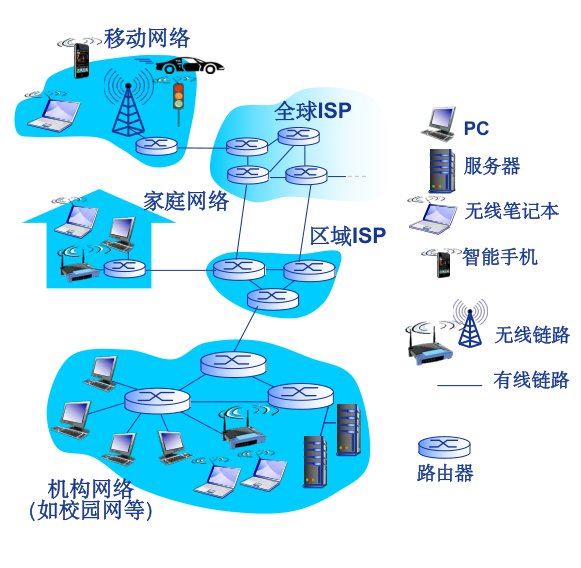
\includegraphics[width=0.82\textwidth]{ch01-internet.png}
  \caption{Internet的组成与互连关系。图中端系统连接家庭、机构、移动和ISP网络；ISP即互联网服务提供商。阅读时可沿链路观察端系统怎样经接入网络进入网络之网络。来源：\texttt{Chapter1-计算机网络概述.pdf}，PDF第8页（课件显示页8），局部截取。}
  \label{fig:ch01-internet}
\end{figure}

\begin{quote}\small\textbf{来源：}课件\texttt{Chapter1-计算机网络概述.pdf}，PDF第4--9页（课件显示页4--9）；参考书第1章§1.1.1--§1.1.3，PDF第12--14页／印刷第1--3页。\end{quote}
\annotationarea[4]

\subsection{网络协议及其三要素}

只把主机、路由器和链路连接起来，不能保证网络应用数据能够按预期交换。网络中的通信实体必须遵循事先约定的规则。\textbf{网络协议}是为网络中的数据交换建立的规则、标准或约定；协议规定通信实体所交换消息的\textbf{格式、含义、顺序}，以及收到消息或发生事件后应采取的动作。

课件把协议要素分为三项：
\begin{itemize}
  \item \textbf{语法（Syntax）}：数据和控制信息的结构或格式，也包括信号电平等表示约定。它回答“消息长什么样”。
  \item \textbf{语义（Semantics）}：控制信息的含义，以及通信实体要执行的动作、响应和差错控制。它回答“收到这条消息应做什么”。
  \item \textbf{时序（Timing）}：事件发生的顺序和速度匹配。它回答“何时发送、先后如何”。
\end{itemize}

课件列出的协议实例包括\textbf{TCP（Transmission Control Protocol，传输控制协议）}、\textbf{IP（Internet Protocol，网际协议）}、\textbf{HTTP（Hypertext Transfer Protocol，超文本传输协议）}和\textbf{802.11无线局域网标准}。Internet标准常通过\textbf{RFC（Request for Comments，请求评论）}文档发布；\textbf{IETF（Internet Engineering Task Force，互联网工程任务组）}参与制定Internet相关标准。RFC是文档系列的名称，不表示每份RFC都是强制标准。

\textbf{区分协议与设备：}设备和链路提供通信的物质基础；协议给通信实体规定交换消息的共同规则。只有链路而没有一致的格式、动作和时序约定，双方就不能可靠地解释收到的数据。

\begin{quote}\small\textbf{来源：}课件\texttt{Chapter1-计算机网络概述.pdf}，PDF第10--16页（课件显示页10--16）；参考书第1章§1.1.2，PDF第13页／印刷第2页。\end{quote}
\annotationarea[4]

\subsection{计算机网络的分类}

课件按三个不同角度分类。它们回答的问题不同，不能把一种角度的类别与另一种角度混为一谈。

\begin{center}
\begin{tabularx}{0.96\textwidth}{l l X}
\toprule
分类角度 & 类别 & 课件给出的含义或范围\\
\midrule
覆盖范围 & PAN（个人区域网） & 约10米\\
 & LAN（局域网） & 约1公里\\
 & MAN（城域网） & 约5--50公里\\
 & WAN（广域网） & 约几十至几千公里\\
使用者 & 专用网（private network） & 供特定组织或用户使用\\
 & 公用网（public network） & 向公众提供网络服务\\
拓扑结构 & 总线、星形、树形、网状 & 描述设备或链路的连接形态\\
\bottomrule
\end{tabularx}
\end{center}

PAN、LAN、MAN、WAN是按覆盖范围划分的网络类别；专用网、公用网按使用者划分；总线、星形、树形、网状按拓扑结构划分。表中距离是课件给出的近似范围，不是所有网络都必须满足的硬性界限。

\begin{quote}\small\textbf{来源：}课件\texttt{Chapter1-计算机网络概述.pdf}，PDF第17页（课件显示页17）。\end{quote}
\annotationarea[4]

\section{计算机网络结构}

\subsection{网络边缘、接入网络与网络核心}

课件把网络结构分成三部分：
\begin{itemize}
  \item \textbf{网络边缘}：主机及其运行的网络应用。用户通过端系统上的应用产生或接收数据。
  \item \textbf{接入网络}：把网络边缘连接到边缘路由器的网络及其物理介质。接入可以使用有线或无线通信链路。
  \item \textbf{网络核心}：互联的路由器或其他分组转发设备构成的网络之网络，负责把数据从源端送往目的端。
\end{itemize}

\textbf{主机}是运行网络应用的端系统。课件介绍两种应用模型：
\begin{itemize}
  \item \textbf{客户/服务器（client/server，C/S）}：客户发送请求，服务器接收请求并返回响应。Web和FTP（File Transfer Protocol，文件传输协议）是课件列出的例子。
  \item \textbf{对等（peer-to-peer，P2P）}：通信在对等实体之间进行，不依赖专用服务器，或不完全依赖专用服务器。课件列举Gnutella、BT（BitTorrent文件共享）、Skype和QQ作为例子。
\end{itemize}

\textbf{接入网络}包括住宅（家庭）接入、机构接入和移动接入。选择接入方式时，课件提示关注数据传输速率（带宽，单位通常为bit/s）以及接入资源是共享还是独占。

\begin{quote}\small\textbf{来源：}课件\texttt{Chapter1-计算机网络概述.pdf}，PDF第19--23页（课件显示页19--23）；参考书第1章§1.1.2，PDF第13页／印刷第2页。\end{quote}
\annotationarea[4]

\subsection{常见接入网络}

课件用家庭、机构和移动接入说明端系统如何连接到网络核心。课件给出的速率是课件材料中的示例数值；实际网络速率会随技术和服务发生变化。

\begin{itemize}
  \item \textbf{数字用户线路（DSL）}：利用已有电话线连接用户侧DSL调制解调器与中心局的DSLAM（DSL接入多路复用器）。数据通信经DSL线路进入Internet；语音经电话网络传输。课件列出的下行速率小于24 Mb/s（典型小于10 Mb/s），上行小于2.5 Mb/s（典型小于1 Mb/s）。课件说明通过频分复用（FDM）把0--4 kHz用于传统电话、4--50 kHz用于上行、50 kHz以上至1 MHz用于下行。
  \item \textbf{电缆网络与HFC}：HFC是混合光纤同轴电缆（hybrid fiber coax）。家庭通过电缆调制解调器连接电缆头端的CMTS（Cable Modem Termination System，电缆调制解调器端接系统），数据再经光纤接入ISP路由器。课件列出的HFC下行速率可达30 Mb/s、上行2 Mb/s，且上下行不对称；多个家庭共享从家庭到电缆头端的接入网络。课件用不同频率传送电视、数据和控制信息。
  \item \textbf{光纤到户（FTTH）}：光纤直接接入家庭。课件区分有源光纤网络（AON）和无源光纤网络（PON）。PON在局端使用光线路终端（OLT），用户侧使用光网络单元（ONU）；光猫ONT是课件举出的ONU类设备例子，线路中可通过无源分光器连接。
  \item \textbf{家庭网络}：课件示意了电话线、有线电视电缆或光纤接入设备，连接家庭路由器、防火墙、网络地址转换（NAT）设备、有线以太网和无线接入点。图中列举的有线以太网速率为1000 Mb/s，无线接入点为866 Mb/s；多个功能可能集成在一个设备盒中。
  \item \textbf{机构以太网接入}：公司、高校等机构内，端系统通常连接以太网交换机，机构路由器再连接ISP。课件列举10 Mb/s、100 Mb/s、1 Gb/s和10 Gb/s等以太网速率。
  \item \textbf{无线接入}：无线局域网在局部范围内通过无线接入点连接端系统；课件将覆盖范围列为同一建筑物内约30 m，并列出802.11ac（Wi-Fi 5）866 Mb/s和Wi-Fi 6最高9.6 Gb/s。蜂窝网络通过运营商基站提供几十公里范围的广域无线接入，课件列出的速率档位为1、10、100 Mb/s和1 Gb/s，并列出3G、4G、5G等移动通信代际。上述速率是课件示例值，不应当作当前实际接入承诺。
\end{itemize}

\begin{quote}\small\textbf{来源：}课件\texttt{Chapter1-计算机网络概述.pdf}，PDF第24--30页（课件显示页24--30）。DSL速率及频带划分见第24页；HFC见第25--26页；FTTH见第27页；家庭、机构和无线接入见第28--30页。\end{quote}
\annotationarea[4]

\subsection{路由与转发}

网络核心需要回答两个不同问题：数据应经过怎样的路径，以及到达一台路由器后应从哪个端口送出。

\textbf{路由（routing）}是确定分组从源到目的传输路径的过程，课件指出可由路由算法确定路径。\textbf{转发（forwarding）}是路由器根据本地转发表，将到达分组从输入端口送到相应输出端口的过程。转发表把目的地址与输出链路对应起来。

路由关注\textbf{端到端路径选择}；转发关注\textbf{当前路由器的一次本地送出}。路由算法决定或更新转发表，转发则在收到分组时查表执行。二者共同构成课件所述网络核心的关键功能。

\begin{figure}[H]
  \centering
  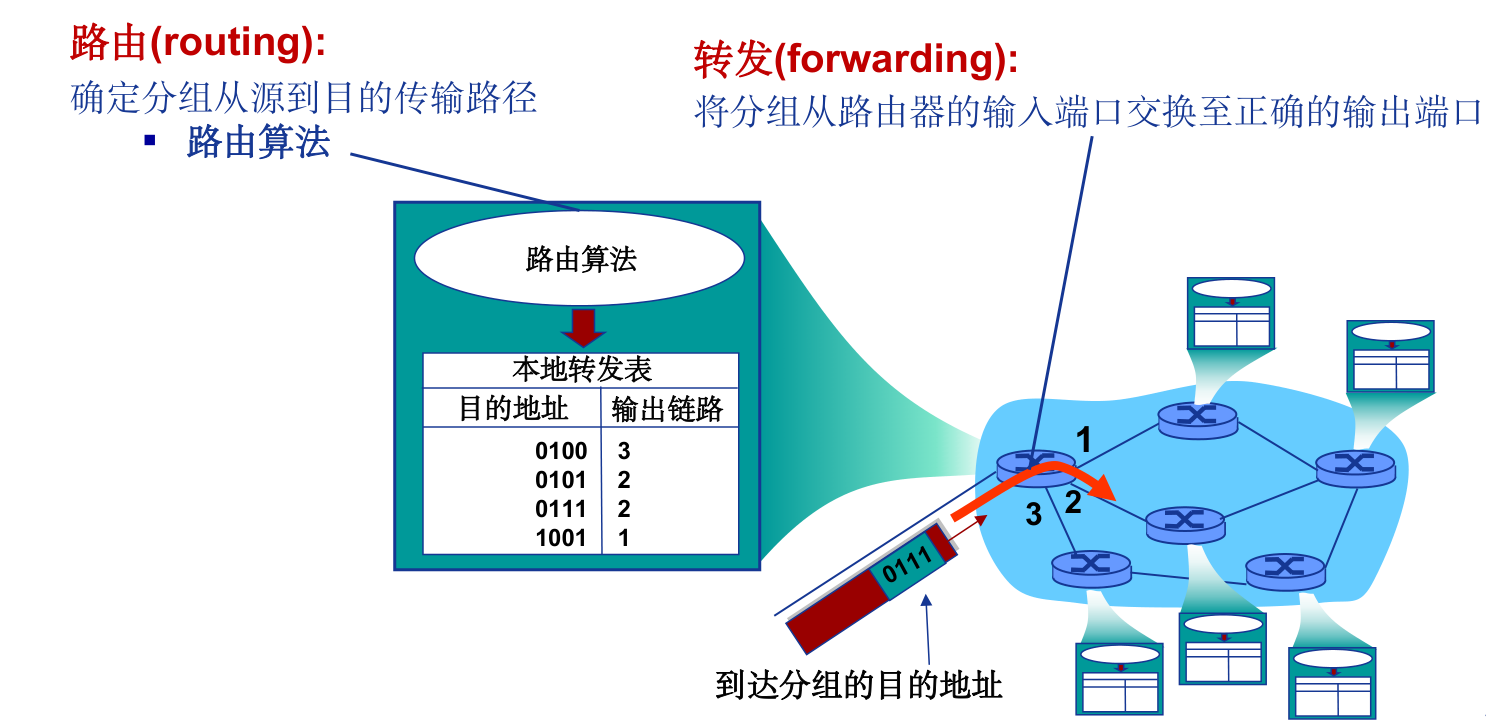
\includegraphics[width=0.82\textwidth]{ch01-routing-review.png}
  \caption{路由和转发的关系。左侧“路由算法”决定路径；右侧路由器按本地转发表把目的地址映射到输出链路。来源：\texttt{Chapter1-计算机网络概述.pdf}，PDF第31页（课件显示页31），局部截取。}
  \label{fig:ch01-routing-forwarding}
\end{figure}

\begin{quote}\small\textbf{来源：}课件\texttt{Chapter1-计算机网络概述.pdf}，PDF第31--32页（课件显示页31--32）；参考书第1章§1.1.2，PDF第13页／印刷第2页。\end{quote}
\annotationarea[4]

\subsection{Internet：网络之网络}

家庭、公司和大学等端系统通常先接入一个\textbf{接入ISP}（Internet Service Provider，互联网服务提供商）。接入ISP还必须继续互连，任意两个主机之间才可能交换分组。大量接入ISP若两两直接互连，网络规模增大时连接数量会急剧增加；对$N$个网络做完全两两连接需要$N(N-1)/2$条连接，数量级为$O(N^2)$。

课件用以下结构说明Internet中的互连关系：
\begin{itemize}
  \item 接入ISP可通过区域ISP连接到更大范围的网络。
  \item 不同ISP之间可通过对等链路（peering link）互连，也可在Internet交换点（IXP，Internet Exchange Point）交换流量。
  \item 少数一级（tier-1）商业ISP提供国家或国际范围的覆盖。
  \item 内容提供商网络（如课件列举的Google网络）可运行自己的网络，连接数据中心并就近提供服务。
\end{itemize}

课件强调Internet是不断演进的复杂“网络之网络”，没有单一、固定的结构图能精确表示所有互连关系。图\ref{fig:ch01-internet}是用于说明组成和关系的示意图。

\begin{quote}\small\textbf{来源：}课件\texttt{Chapter1-计算机网络概述.pdf}，PDF第33--41页（课件显示页33--41）。\end{quote}
\annotationarea[4]

\section{数据交换}

\subsection{为什么需要数据交换}

若每对主机都用一条专用链路直接互连，主机数量增多时，所需链路数量会迅速增加，而且链路资源难以共享。\textbf{交换网络}通过交换节点连接多台主机：数据进入网络后，由节点选择或使用相应链路送往目的端。课件将交换方式分为\textbf{电路交换、报文交换和分组交换}。

\begin{quote}\small\textbf{来源：}课件\texttt{Chapter1-计算机网络概述.pdf}，PDF第43--49页（课件显示页43--49）；参考书第1章§1.1.4，PDF第14--16页／印刷第3--5页。\end{quote}
\annotationarea[4]

\subsection{电路交换、报文交换与分组交换}

\begin{center}
\begin{tabularx}{0.98\textwidth}{l X X X}
\toprule
 & 电路交换 & 报文交换 & 分组交换\\
\midrule
传送单位 & 建立的端到端电路承载连续比特流 & 报文，即应用发送的信息整体 & 报文拆分得到的较小分组\\
开始发送前 & 先建立连接、占用资源 & 不需建立连接 & 不需建立连接\\
转发方式 & 建立电路后沿专用路径传输 & 节点完整接收一个报文后再转发 & 节点收到并存储分组后逐个转发\\
资源使用 & 通信期间独占所分配资源 & 报文传送时占用链路 & 分组传送时占用链路，可统计共享\\
结束时 & 释放连接和资源 & 无需拆除电路 & 无需拆除电路\\
\bottomrule
\end{tabularx}
\end{center}

\textbf{电路交换}最典型的例子是电话网络。其三个阶段是\textbf{建立连接（呼叫/电路建立）—通信—释放连接}。通信双方在数据传输前建立专用端到端通路，并在通信期间独占分配给该通路的资源。课件指出可用时分复用（TDM，Time-Division Multiplexing）或频分复用（FDM，Frequency-Division Multiplexing）让多路通信共享链路的不同时间片或频带；具体复用方式在物理层章节展开。

\textbf{报文交换}把源应用发送的信息整体作为一个报文，例如一个文件或一张图像。交换节点必须先完整接收并存储报文，再向下一跳转发。这会产生较大的存储转发等待，并要求节点能存下完整报文。

\textbf{分组交换}先把报文拆成较小的数据块，并在每块前添加首部等控制信息，形成分组；目的端再根据分组信息重组报文。拆装和添加首部会增加开销。节点按分组存储转发，不必等待整个报文到达后才开始转发，因此多个分组可以在不同链路上形成流水传输。

\textbf{统计多路复用（statistical multiplexing）}是分组交换共享链路的方式：有分组需要传送时才竞争使用链路，链路带宽不按用户永久切分。它适合突发数据并能提高资源共享程度；当到达流量超过链路和缓存的承受能力时，也可能出现分组排队、延迟和丢失。因此课件明确提出，分组交换并非在所有服务目标下都优于电路交换；需要带宽保障的音频或视频业务还要考虑性能保障机制。课件第74页提出“如何提供电路级性能保障”。\textbf{参考书补充（本课件未展开）：}若要在分组网络中承诺带宽，建立业务时应检查路径各链路是否有足够可用容量，并为获准业务预留资源；容量不足时拒绝接入或降低承诺。虚电路能固定转发路径，但路径固定本身不等于带宽预留；多个虚电路仍可共享链路。

\begin{quote}\small\textbf{来源：}课件\texttt{Chapter1-计算机网络概述.pdf}，PDF第46--58、73--74页（课件显示页相同）；参考书第1章§1.1.4，PDF第14--16页／印刷第3--5页；虚电路与数据报的差别见第4章§4.1.3，PDF第140--142页／印刷第129--131页。课件第53页将英文写作“package switching”；本笔记按课件中文术语“分组交换”书写。\end{quote}
\annotationarea[4]

\subsection{发送时延、存储转发和流水传输}

\textbf{发送时延（传输时延）}是把一个分组的全部比特推入链路所需的时间。设分组长$L$ bit、链路传输速率$R$ bit/s，则
\[
 t_{\mathrm{trans}}=\frac{L}{R}\quad(\mathrm{s}).
\]
此处$L$计量分组长度，$R$计量每秒可发送的比特数，结果单位是秒。它不是信号在链路中跑完距离所需的时间；传播时延将在性能部分定义。

对报文长度$M$ bit、分组长度$L$ bit、每条链路速率均为$R$的存储转发网络，若路径含$h$段链路（$n=h-1$个路由器），忽略传播、处理和排队时延，分组长度一致且$M$可被分组有效长度整除，则课件给出的流水传输完成时间为
\[
T=\frac{M}{R}+(h-1)\frac{L}{R}
 =\frac{M}{R}+n\frac{L}{R}.
\]
首项是源端发送全部数据所需时间；其余$h-1$项是末尾分组在中间路由器逐跳转发所增加的时间。该式解释了分组流水：第一个分组先经过各跳，后续分组可在前一分组已经进入下一链路时继续从源端发送。

\textbf{课件例题：报文交换与分组交换}（PDF第60--69页）。给定报文$M=7.5$ Mbit、分组长$L=1500$ bit、三段等速率链路$R=1.5$ Mbit/s，求报文从源端发送至目的端的时间，并比较交换节点所需的最小缓存。

\textbf{解：}
\begin{enumerate}
  \item 分组数为$M/L=7.5\times10^6/1500=5000$。
  \item 报文交换中，每个中间节点先接收整个报文。每段链路发送整个报文的时间是$M/R=7.5/1.5=5$ s；三段链路依次存储转发，总时间为$3\times5=15$ s。
  \item 分组交换中，单个分组的发送时延为$L/R=1500/(1.5\times10^6)=0.001$ s，即1 ms。课件图给出的流水完成时间为$5002$ ms，也可由$M/R+(3-1)L/R=5+0.002=5.002$ s得到。
  \item 若问题问“至少要能存下一个完整的待转发单位”，报文交换节点需能存下整个报文$M=7.5$ Mbit；分组交换节点需能存下一个完整分组$L=1500$ bit。实际队列总缓存大小还取决于同时排队的分组数量，课件数据不足以计算该总量。
\end{enumerate}
\annotationarea[4]

\begin{quote}\small\textbf{来源：}课件\texttt{Chapter1-计算机网络概述.pdf}，PDF第59--70页（课件显示页59--70）；参考书第1章§1.1.4，PDF第15--16页／印刷第4--5页。\end{quote}
\annotationarea[4]

\subsection{课件例题1：文件经两台路由器传送}

\textbf{题目}（课件例1，PDF第71页）：采用存储转发的分组交换网络中，所有链路速率为100 Mb/s。每个分组总长1000 B，分组头20 B。主机$H_1$向$H_2$发送980000 B文件，路径经过两个路由器。忽略分组拆装时间和传播时延，求从$H_1$开始发送到$H_2$接收完所需的最短时间。

\textbf{解：}每个分组可承载的文件数据为$1000-20=980$ B，因此分组数为$980000/980=1000$。每个分组在线路上仍占1000 B，故$H_1$发送完全部分组需要
\[
 t_{H_1}=\frac{1000\times1000\times8}{100\times10^6}\ \mathrm{s}
 =0.080\ \mathrm{s}=80\ \mathrm{ms}.
\]
在速率相同的链路上，分组流水传输时，最后一个分组还要经过两个路由器转发；增加的时间为
\[
 t_{\mathrm{extra}}=2\times\frac{1000\times8}{100\times10^6}\ \mathrm{s}
 =0.00016\ \mathrm{s}=0.16\ \mathrm{ms}.
\]
所以$H_2$接收完整个文件至少需$80+0.16=80.16$ ms。这里计算的是分组总长（含分组头）的链路占用时间；忽略题目明确排除的拆装和传播时间。
\annotationarea[4]

\begin{quote}\small\textbf{来源：}课件\texttt{Chapter1-计算机网络概述.pdf}，PDF第71--72页（课件显示页71--72）；参考书第1章§1.1.4同类存储转发计算，PDF第15--16页／印刷第4--5页。\end{quote}
\annotationarea[4]

\subsection{课件例题：分组交换与电路交换的资源共享}

\textbf{题目}（课件PDF第73页）：一条1 Mb/s链路上，每个用户活动时需100 kb/s，平均活动时间占10\%。电路交换可支持多少用户？35个用户使用分组交换时，超过10人同时活动的概率是多少？

\textbf{解：}电路交换需要为每个用户预留100 kb/s，因此$1$ Mb/s$/100$ kb/s$=10$个用户。分组交换不为每位用户永久预留全部活动速率；若额外假设各用户是否活动相互独立，令同时活动人数为随机变量$X$，则$X$服从参数$n=35,p=0.1$的二项分布。超过10人同时活动的概率为
\[
\Pr(X>10)=\sum_{k=11}^{35}{35\choose k}(0.1)^k(0.9)^{35-k}
\approx 0.0004243.
\]
该数约为$4.24\times10^{-4}$。课件写作“$<0.0004$”；按上述独立二项模型精算，该严格不等式不成立，$0.0004243$可粗略写成$0.0004$（保留一位有效数字）。课件未明说独立性，这是计算该概率所需的建模前提。分组交换因用户并非总在活动，可让更多用户共享链路，但超过链路能力时仍会排队或丢包。
\annotationarea[4]

\begin{quote}\small\textbf{来源与核对：}课件\texttt{Chapter1-计算机网络概述.pdf}，PDF第73--74页（课件显示页73--74）。课件给出“$<0.0004$”；按独立活动假设求二项分布尾概率为约$0.0004243$，故这里保留课件数值并说明精算差异。\end{quote}
\annotationarea[4]

\section{计算机网络性能指标}

\subsection{速率、带宽与吞吐量}

\textbf{速率}即数据率或比特率，表示单位时间传输的数据量，是课件列出的重要性能指标。课件此处按十进制使用$1$ kb/s$=10^3$ bit/s、$1$ Mb/s$=10^6$ bit/s、$1$ Gb/s$=10^9$ bit/s、$1$ Tb/s$=10^{12}$ bit/s。课件还指出，速率往往指额定或标称速率。注意bit（比特）与B（字节）不同：$1$ B$=8$ bit。网络语境下“带宽”常指数字信道可传送的最高数据率，单位为bit/s；信号语境中的频带宽度是最高频率与最低频率之差，单位为Hz，两种语境不可混用。

\textbf{吞吐量（throughput）}是发送端与接收端之间实际传送数据的速率。\textbf{即时吞吐量}描述某一时刻的速率；\textbf{平均吞吐量}是在一段时间内平均得到的速率。路径上的链路速率可能不同，端到端吞吐量受瓶颈链路限制。若服务器侧速率为$R_s$、客户侧速率为$R_c$，且路径中间链路速率为$R$并由10条连接平均共享，课件给出的每条连接吞吐量为
\[
\min(R_c,R_s,R/10).
\]
\textbf{课件提示题：}若$R_s<R_c$，端到端吞吐量受$R_s$限制；若$R_s>R_c$，则受$R_c$限制。共同原则是取端到端路径中可用速率的最小值。

\begin{quote}\small\textbf{来源：}课件\texttt{Chapter1-计算机网络概述.pdf}，PDF第77--78、88--90页（课件显示页77--78、88--90）；参考书第1章§1.1.5，PDF第17--19页／印刷第6--8页。\end{quote}
\annotationarea[4]

\subsection{结点时延与分组丢失}

分组经过结点时会经历四类时延。设分组长$L$ bit、输出链路速率$R$ bit/s、链路长度$d$ m、信号传播速度$s$ m/s，则
\[
\begin{aligned}
 d_{\mathrm{nodal}}&=d_{\mathrm{proc}}+d_{\mathrm{queue}}+d_{\mathrm{trans}}+d_{\mathrm{prop}},\\
 d_{\mathrm{trans}}&=\frac{L}{R},\qquad
 d_{\mathrm{prop}}=\frac{d}{s}.
\end{aligned}
\]
各量的含义如下：
\begin{itemize}
  \item \textbf{处理时延}$d_{\mathrm{proc}}$：结点检查分组首部、进行差错检测、确定输出端口等处理所需的时间。课件指出通常小于毫秒。
  \item \textbf{排队时延}$d_{\mathrm{queue}}$：分组在输出队列中等待链路可用的时间，取决于到达流量和队列状态。
  \item \textbf{发送时延}$d_{\mathrm{trans}}$：把分组全部比特发送到链路上所需时间。它由分组长度和链路速率决定。
  \item \textbf{传播时延}$d_{\mathrm{prop}}$：信号沿物理介质传播所需时间。它由链路长度和介质中的传播速度决定。
\end{itemize}

课件以$2\times10^8$ m/s作为链路信号传播速度的近似值。\textbf{发送时延和传播时延不是一回事：}增大速率$R$会缩短发送时延；缩短距离$d$或提高传播速度$s$会缩短传播时延。处理与排队则发生在结点。

\begin{figure}[H]
  \centering
  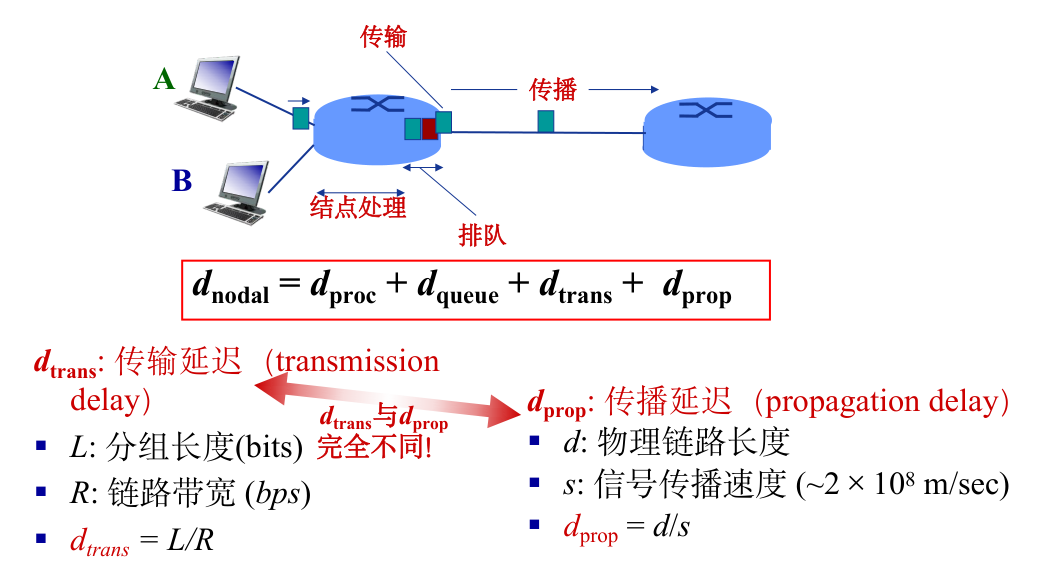
\includegraphics[width=0.82\textwidth]{ch01-delay.png}
  \caption{结点的四类时延及其合成关系。图中$d_{\mathrm{trans}}$表示把整包比特送入链路的过程，$d_{\mathrm{prop}}$表示信号在链路中传播的过程。来源：\texttt{Chapter1-计算机网络概述.pdf}，PDF第81页（课件显示页81），局部截取。}
  \label{fig:ch01-delay}
\end{figure}

\textbf{排队流量强度}用于描述分组到达速率与链路服务能力的关系。令$a$为平均分组到达速率（packet/s），$L$为平均分组长度（bit），$R$为链路速率（bit/s），则
\[
\rho=\frac{La}{R}.
\]
$La$是平均到达的比特速率。课件指出：$\rho$接近0时平均排队时延很小；$\rho$接近1时平均排队时延会很大；$\rho>1$时到达速率超过链路处理能力，在理想无限队列模型下平均排队时延发散，实际有限队列会导致丢包。

课件用车队类比区分发送与传播：收费站放行一辆车所需时间对应发送一个比特的时间；车队中每辆车对应一个比特，整队通过收费站所需时间对应分组发送时延；车从一个收费站行驶到下一个收费站的时间对应传播时延。课件例子中车队由10辆车组成、每辆放行需12秒，整队通过需120秒；两站相距100 km、车速100 km/h，单车到下一站需1小时。这个类比表明，队列整体通过服务点的时间与每个车/比特在路径上行进的时间是两种不同量。

\textbf{分组丢失（丢包）}：路由器队列缓存容量有限；如果新分组到达时队列已满，该分组可能被丢弃。丢弃的分组可能由前序结点或源端重发，也可能不重发。课件定义
\[
\text{丢包率}=\frac{\text{丢包数}}{\text{已发送分组总数}}.
\]

\begin{quote}\small\textbf{来源：}课件\texttt{Chapter1-计算机网络概述.pdf}，PDF第79--83、87页（课件显示页79--83、87）；参考书第1章§1.1.5，PDF第18--19页／印刷第7--8页。\end{quote}
\annotationarea[4]

\subsection{时延带宽积、往返时间和利用率}

若传播时延为$d_{\mathrm{prop}}$、链路速率为$R$ bit/s，\textbf{时延带宽积}为
\[
  d_{\mathrm{prop}}R\quad(\text{bit}).
\]
它表示信号传播期间，链路中能够容纳的比特数量；单位是bit。课件把它称为“以比特为单位的链路长度”。

\textbf{往返时间（RTT，Round-Trip Time）}的口径在不同材料中不同。课件第85页把RTT定义为从发送方发送完数据到开始收到确认数据所经历的时间；ACK（acknowledgment，确认）是接收方发回的确认分组。课件用简化式
\[
\mathrm{RTT}=t_P+t_{\mathrm{PRC}}+t_P=2t_P+t_{\mathrm{PRC}}
\]
表示：$t_P$是单向传播时延，$t_{\mathrm{PRC}}$是接收方处理时延；此简化式未计中间结点时延。课件接着写出响应时间
\[
T_{\mathrm{response}}=t_{\mathrm{PKT}}+\mathrm{RTT}+t_{\mathrm{ACK}},
\]
其中$t_{\mathrm{PKT}}$、$t_{\mathrm{ACK}}$分别表示数据分组和确认分组的发送时延。

参考书对RTT的定义是：从发送端发出一个短分组到收到接收端确认所经历的时间；包含往返传播时延、接收端处理时延以及互联网中间节点的处理和排队时延，但不包括数据分组本身的发送时延（参考书第1章§1.1.5，PDF第19页／印刷第8页）。实际题目须按题目或课件给定口径判断是否计入发送、排队及中间处理时延；本章课堂公式以PPT的简化口径为主。

\textbf{信道利用率}是信道被使用的时间占总时间的比例；课件把\textbf{网络利用率}定义为全网络各信道利用率的加权平均。课件第86页停等图的公式图像存在疑似笔误：分子是$t_{\mathrm{PKT}}$，但分母显示为$t_{\mathrm{ACK}}+\mathrm{RTT}+t_{\mathrm{ACK}}$；这与相邻第85页的响应时间表达式不一致。若用“发送数据分组的时间/一个完整发送周期”计算停等发送方利用率，且周期由数据发送、RTT和ACK发送组成，则一致的计算式应为
\[
U=\frac{t_{\mathrm{PKT}}}{t_{\mathrm{PKT}}+\mathrm{RTT}+t_{\mathrm{ACK}}}.
\]
这里将课件疑似笔误明确标出，不能把第86页图上分母原样当作正确结果。不同教材可能对利用率、响应时间和RTT的计时起点作不同约定，计算时应先列出一个周期所包含的事件。

\begin{figure}[H]
  \centering
  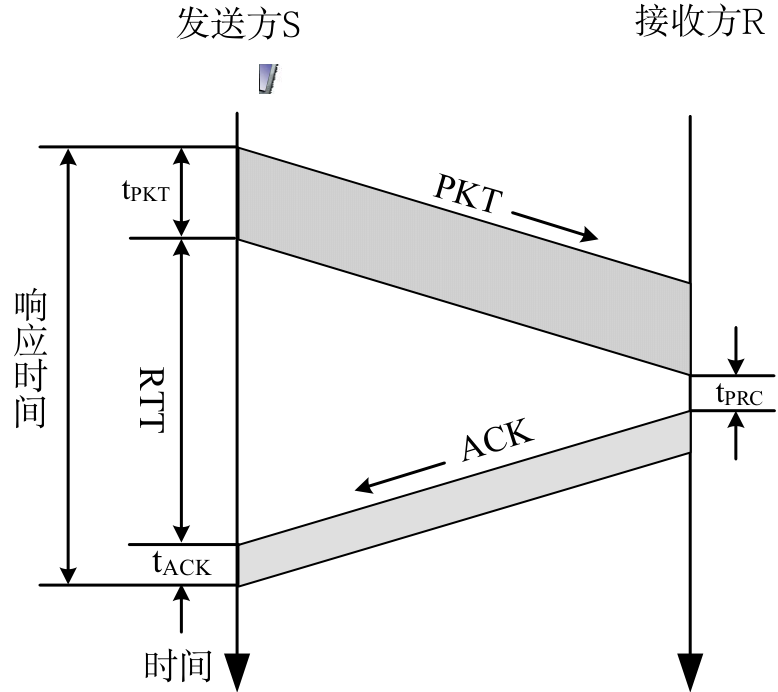
\includegraphics[width=0.80\textwidth]{ch01-rtt-review.png}
  \caption{课件的RTT与响应时间示意。数据分组由S发往R，R处理后返回ACK；图中$t_{\mathrm{PKT}}$和$t_{\mathrm{ACK}}$是发送时间，斜向传播段体现传播时间。来源：\texttt{Chapter1-计算机网络概述.pdf}，PDF第85页（课件显示页85），局部截取。}
  \label{fig:ch01-rtt}
\end{figure}

\begin{quote}\small\textbf{来源与核对：}课件\texttt{Chapter1-计算机网络概述.pdf}，PDF第84--86页（课件显示页84--86）；参考书第1章§1.1.5，PDF第19--20页／印刷第8--9页。PPT与参考书的RTT定义范围不同；PPT第86页利用率公式分母与第85页响应时间式不一致，正文按事件周期给出一致式并保留差异说明。\end{quote}
\annotationarea[4]

\subsection{课件例题2：吞吐量、完成时间与路由器排队}

\textbf{题目}（课件例2，PDF第91页）：主机A经路由器R1、R2连接主机B，A以存储转发方式发送大文件。课件文字给出的三段链路速率依次为100 kb/s、2 Mb/s和1 Mb/s。求无其他流量时最大吞吐量；文件为4 MB时的传输时间；分组是否排队以及排队位置。

\textbf{（1）最大吞吐量。} 端到端吞吐量由最慢链路限制：
\[
\min(100\ \mathrm{kb/s},2\ \mathrm{Mb/s},1\ \mathrm{Mb/s})=100\ \mathrm{kb/s}.
\]

\textbf{（2）文件传输时间。} 课件注释$1$ k$=10^3$、$1$ M$=10^6$，因此$4$ MB$=4\times10^6$ B$=32\times10^6$ bit。按瓶颈吞吐量估算，
\[
T=\frac{32\times10^6\ \mathrm{bit}}{100\times10^3\ \mathrm{bit/s}}=320\ \mathrm{s}.
\]
该估算适用于大文件稳态传输并忽略起始流水填充等附加时间，符合课件给出的近似题意。

\textbf{（3）排队位置及资料冲突。} 课件第91页文字按A至B顺序写100 kb/s、2 Mb/s、1 Mb/s；但同页网络图及第94页排队图画的是1 Mb/s、2 Mb/s、100 kb/s。图示局部如下：
\begin{figure}[H]
  \centering
  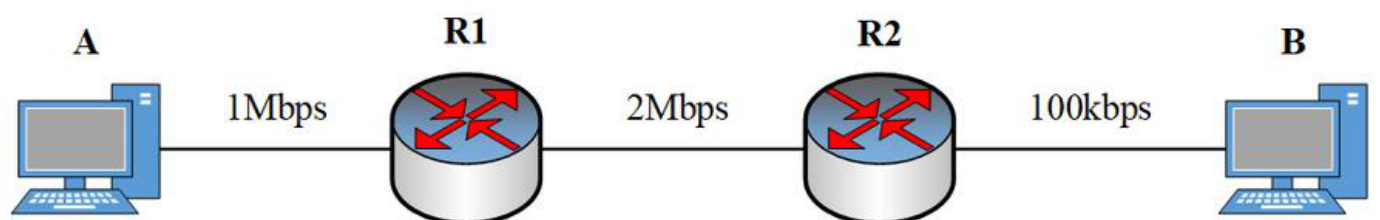
\includegraphics[width=0.80\textwidth]{ch01-throughput-example.png}
  \caption{课件例2的链路速率图。按图示方向，A--R1为1 Mb/s、R1--R2为2 Mb/s、R2--B为100 kb/s。来源：\texttt{Chapter1-计算机网络概述.pdf}，PDF第91页（课件显示页91），局部截取。}
  \label{fig:ch01-throughput-example}
\end{figure}
按图示顺序，分组到达R2的速度快于R2向100 kb/s末段链路发送的速度，故持续发送时会在R2输出队列排队；这与课件第94页给出的“在R2发生排队”相符。若按第91页文字顺序理解，即第一段已是100 kb/s、后续链路更快，则持续分组的到达间隔由慢速第一段决定，后续链路能更快服务，不会因这三段速率关系在R1或R2形成持续排队。两种读法的瓶颈吞吐量和大文件近似时间相同，但排队位置结论不同；本笔记保留这一处课件图文冲突，不把图和文字混用。
\annotationarea[4]

\begin{quote}\small\textbf{来源与核对：}课件\texttt{Chapter1-计算机网络概述.pdf}，PDF第91--94页（课件显示页91--94）。第91页文字与网络图的速率顺序不一致；第94页“在R2排队”的答案与图示顺序相符。参考书第1章§1.1.5关于瓶颈链路的说明，PDF第19页／印刷第8页。\end{quote}
\annotationarea[4]

\section{计算机网络体系结构}

\subsection{分层结构、实体、协议、服务与接口}

计算机网络涉及主机、路由器、链路、应用、协议、硬件和软件等大量部分。\textbf{分层结构}把复杂系统拆成若干层，每层完成一类功能，使用下层提供的服务，并向上层提供服务。分层有助于描述系统、模块化设计、维护更新和标准化；改变某层的实现时，只要其服务约定不变，上下层通常不必了解其内部实现。

\textbf{网络体系结构}是计算机网络各层及其协议的集合，是从功能角度描述网络层次及其相互关系的抽象结构。层次模型规定功能边界，不等同于具体设备中软件和硬件模块的唯一划分。

课件指出分层使结构清晰、便于模块更新维护，并有利于标准化；同时在第99页提出“分层是否有不利之处”但未直接作答。结合课件第105页说明的封装过程可知，逐层添加控制信息会增加传输开销；课件没有在本章系统展开其他缺点。

课件第100页给出以下基本概念：
\begin{itemize}
  \item \textbf{实体（entity）}：任何可发送或接收信息的硬件或软件进程。
  \item \textbf{对等实体}：位于不同系统、处于相同层次并按同层协议通信的实体。它们遵循的协议是逻辑上“水平”的。
  \item \textbf{服务}：某层向其上一层提供的功能。服务使用关系是相邻层之间“垂直”的；上层使用服务，不必了解下层如何实现。
  \item \textbf{接口}：同一系统中相邻层实体交换信息的边界。
  \item \textbf{服务访问点（SAP，Service Access Point）}：上层实体访问下层服务的位置；双方通过服务原语请求或使用特定服务。
\end{itemize}

\begin{figure}[H]
  \centering
  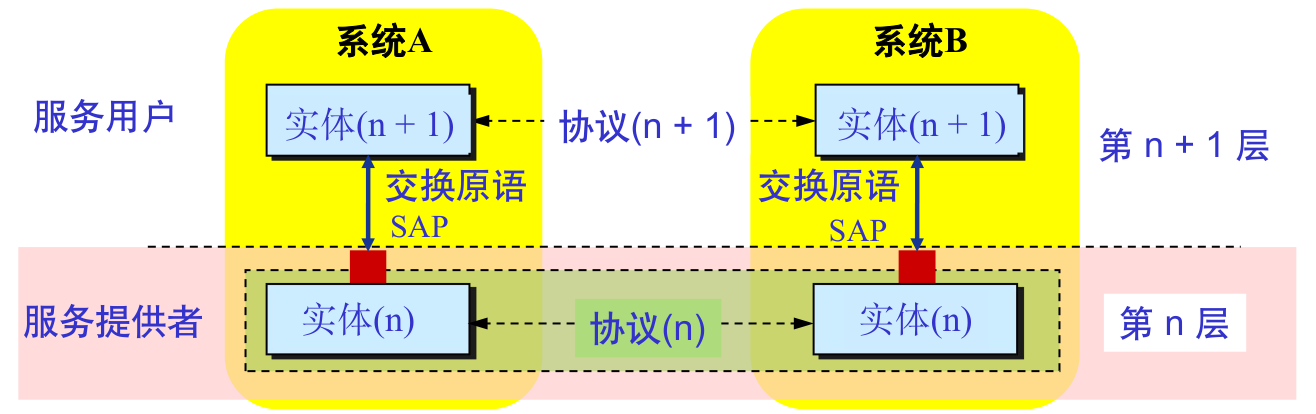
\includegraphics[width=0.82\textwidth]{ch01-layer-services-review.png}
  \caption{对等协议、层间服务和SAP。左右系统中同层实体按协议交换信息；每个系统内部由下层向相邻上层提供服务，SAP是服务访问位置。来源：\texttt{Chapter1-计算机网络概述.pdf}，PDF第100页（课件显示页100），局部截取。}
  \label{fig:ch01-layer-service}
\end{figure}

\textbf{协议数据单元（PDU）}是某层按本层协议处理和交换的数据单位。封装时，下层在上层数据外加入本层需要的控制信息，例如标识发送端或接收端的地址、用于差错检测或纠正的编码，以及实现协议功能的控制信息（如优先级、服务质量和安全控制）。PPT第105页将这些控制信息作为构造PDU的原因。

\begin{quote}\small\textbf{来源：}课件\texttt{Chapter1-计算机网络概述.pdf}，PDF第96--100、104--105页（课件显示页96--100、104--105）；参考书第1章§1.2.1，PDF第26--29页／印刷第15--18页。\end{quote}
\annotationarea[4]

\subsection{OSI七层参考模型及各层功能}

国际标准化组织（ISO）于1984年提出\textbf{开放系统互连（OSI）参考模型}，用于描述异构系统怎样互连。它是理解网络通信的理论模型，课件指出“理论成功，市场失败”。OSI自下而上共七层：

\begin{center}
\begin{tabularx}{0.98\textwidth}{c l X}
\toprule
层号 & 层名 & 课件所列主要功能\\
\midrule
7 & 应用层 & 为用户程序提供网络服务；例：HTTP、FTP、SMTP。\\
6 & 表示层 & 处理信息表示的语法和语义；可进行主机无关格式转换、编码、加密/解密、压缩/解压缩。\\
5 & 会话层 & 管理对话；建立和维护会话；在数据流中插入同步点。\\
4 & 传输层 & 提供源到目的端的进程间完整报文传输；分段与重组、SAP寻址、连接控制、流量控制和差错控制。\\
3 & 网络层 & 负责源主机到目的主机的分组传送，可能穿越多个网络；逻辑寻址（例如IP地址）、路由和转发。\\
2 & 数据链路层 & 负责相邻结点间传输；组帧、物理寻址、流量控制、差错控制、介质访问控制。\\
1 & 物理层 & 在物理介质上发送比特；规定接口特性、比特编码、数据率、时钟同步和传输模式：单工只单向传输，半双工双方轮流，全双工双方可同时传输。\\
\bottomrule
\end{tabularx}
\end{center}

\textbf{按通信范围辨别层次：}数据链路层处理相邻结点之间的传输；网络层把分组从源主机送到目的主机，可能经过多个网络；传输层面向不同主机上的应用进程，处理端到端传输。应用层与用户可见的网络服务相邻。课件列出的数据链路层差错控制和传输层差错控制处于不同通信范围，不应混为一个功能。

数据链路层的流量控制用于避免发送方“淹没”接收方；差错控制用于检测损坏或丢失帧，并可重传、避免重复帧；介质访问控制用于决定共享链路在给定时刻由哪个设备使用。传输层的SAP寻址要把完整报文交给正确进程，课件以端口号为例；分段与重组、连接控制、流量控制和差错控制面向源到目的的进程通信。

\textbf{数据封装}发生在发送端：上层数据逐层向下交付，各层根据协议加入本层控制信息，形成相应PDU；接收端逐层向上处理并移除对应控制信息。传输过程中，中间系统只需实现转发所需的层次，不必像端系统那样处理全部应用层功能。

\begin{quote}\small\textbf{来源：}课件\texttt{Chapter1-计算机网络概述.pdf}，PDF第101--115页（课件显示页101--115）；参考书第1章§1.2.2，PDF第29--34页／印刷第18--23页。\end{quote}
\annotationarea[4]

\subsection{TCP/IP模型与五层参考模型}

课件给出的\textbf{TCP/IP（传输控制协议/网际协议）模型}自上而下为\textbf{应用层、传输层、网际层、网络接口层}。网络接口层连接具体网络技术；网际层中的IP为不同应用和网络提供互联服务。课件用“Everything over IP”和“IP over Everything”概括：IP可为各种应用提供服务，也可运行在多种网络技术之上。

用于学习网络通信过程时，课件还介绍综合OSI和TCP/IP模型优点的\textbf{五层参考模型}：
\begin{itemize}
  \item \textbf{应用层}：支持网络应用，如FTP（文件传输协议）、SMTP（Simple Mail Transfer Protocol，简单邮件传输协议）、HTTP（超文本传输协议）。
  \item \textbf{传输层}：负责进程到进程的数据传输，如TCP和UDP（User Datagram Protocol，用户数据报协议）。
  \item \textbf{网络层}：负责源主机到目的主机的分组传送、路由和转发，如IP。
  \item \textbf{数据链路层}：负责相邻网络元素之间的数据传输，如以太网、802.11（Wi-Fi）和PPP。
  \item \textbf{物理层}：负责比特传输。
\end{itemize}

\textbf{五层模型的PDU名称}按课件第119页为：应用层\textbf{报文（message）}，传输层\textbf{段（segment）}，网络层\textbf{数据报（datagram）}，数据链路层\textbf{帧（frame）}，物理层传送\textbf{比特（bits）}。封装时每层加入本层首部等信息；路由器按课件图处理到网络层并在相邻链路上重新封装帧，交换机处理数据链路层和物理层；端系统运行完整五层模型。

\begin{figure}[H]
  \centering
  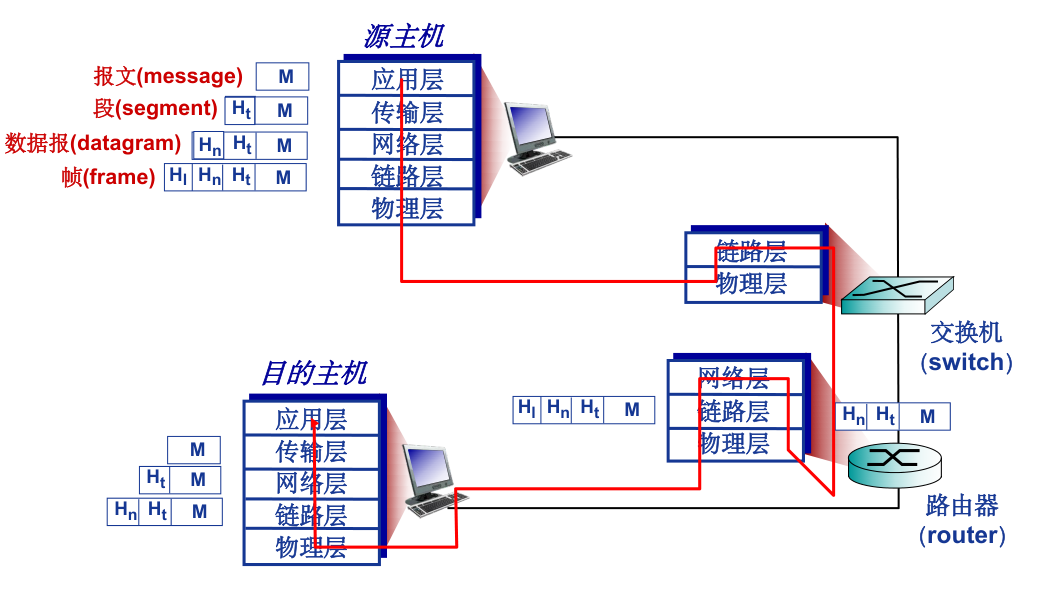
\includegraphics[width=0.84\textwidth]{ch01-encapsulation.png}
  \caption{五层模型下的封装与中间设备处理范围。应用数据逐层加入首部成为段、数据报和帧，最终变成比特；路由器转发网络层数据，交换机按链路层信息转发帧。来源：\texttt{Chapter1-计算机网络概述.pdf}，PDF第119页（课件显示页119），局部截取。}
  \label{fig:ch01-encapsulation}
\end{figure}

\begin{quote}\small\textbf{来源：}课件\texttt{Chapter1-计算机网络概述.pdf}，PDF第116--119页（课件显示页116--119）；参考书第1章§1.2.2，PDF第34--38页／印刷第23--27页。\end{quote}
\annotationarea[2]

\section{计算机网络发展历史（课件标注“略”）}

\subsection{课件时间线}

本节按课件列出的里程碑整理，课件第120页将其标注为“略”。年份和事件是帮助识别发展阶段的时间线，不替代各协议的后续章节。

\begin{center}\small
\begin{tabularx}{0.96\textwidth}{l X}
\toprule
时期 & 课件列出的事件\\
\midrule
1961--1972 & 1961年Kleinrock用排队论分析分组交换有效性；1964年Baran研究分组交换在军事网络中的应用；1967年美国高级研究计划局（ARPA，Advanced Research Projects Agency）提出ARPAnet构想；1969年首个ARPAnet结点运行。1972年ARPAnet公开演示，出现第一个主机到主机协议NCP（Network Control Protocol，网络控制协议）和第一个电子邮件程序，ARPAnet有15个结点。\\
1972--1980 & 1970年ALOHA卫星网络建成；1974年Cerf与Kahn提出网络互连体系结构；1975年ARPAnet移交美国国防部通信局管理；1976年Xerox设计以太网；20世纪70年代后期出现DECnet、SNA、XNA等私有体系结构及固定长度分组交换（ATM，异步传递模式的先驱）；1979年ARPAnet有200个结点。课件概括的互连原则包括极简、自治、尽力服务、无状态路由器和分散控制。\\
1980--1990 & 1982年定义SMTP（Simple Mail Transfer Protocol，简单邮件传输协议）；1983年部署TCP/IP并定义DNS（Domain Name System，域名系统）；1985年定义FTP；1986年美国国家科学基金会网络（NSFnet）形成骨干网、区域网和校园网组成的三级网络；1988年出现TCP拥塞控制。课件还列出CSnet、BITnet、NSFnet、Minitel等新型网络，以及当时约10万台主机连接公共网络。\\
1990--2000年代 & 20世纪90年代初ARPAnet退役；1991年NSF解除NSFnet商业应用限制，NSFnet于1995年退役并由私营企业经营；1992年Internet Society（ISOC，互联网协会）成立。Web依托超文本（Bush于1945年、Nelson于20世纪60年代提出相关思想）、HTML和HTTP发展；1994年出现Mosaic和Netscape浏览器，90年代后期Web开始商业应用。课件还列出即时消息、P2P文件共享、网络安全、主机约5万和用户逾1亿等历史数据，以及Gb/s级网络主干。\\
2005年至今（按课件表述） & 宽带接入和高速无线接入增长；课件列出约50亿台移动终端（2016年）和38.9亿互联网用户（2018年）等当时统计；社交网络发展，课件列举Facebook用户很快达到10亿；Google、Microsoft等服务提供商建设专用网络；电子商务、大学和企业把服务运行在Amazon EC2、Azure等云平台中。上述数字仅是课件所列历史统计，不代表当前数据。\\
\bottomrule
\end{tabularx}
\end{center}

\begin{quote}\small\textbf{来源：}课件\texttt{Chapter1-计算机网络概述.pdf}，PDF第120--125页（课件显示页120--125）；其中第120页标题明确标注“略”。\end{quote}


% 第2章：依课件2.1--2.8顺序整理；标注课件例题、参考书补充及必要核对说明。
\chapter{物理层}

\noindent\textbf{本章要解决的问题。} 上一章把一条链路看成能够发送比特的通道，本章打开这条通道：0和1怎样变成线路上的信号，接收方怎样认出它们，什么限制传输速率，多路通信怎样共用一条线路。物理层向数据链路层提供比特流传输能力；至于这些比特组成什么帧、属于哪个地址，将在下一章讨论。

\noindent\textbf{阅读提示。} 按课件的八节顺序学习。先把数据、信号、码元、比特率和波特率分清，再使用容量公式；看到波形时先找时间边界，看到公式时先核对单位。本章的“学习补充”和“自拟例”用于解释必要基础，不作为课件原题或课堂原话。

\section{物理层基本功能}
\subsection{从比特到信号：物理层做什么}
计算机内部保存的比特只有0和1，但一根导线不会直接运输抽象的数字。发送端必须选择一种物理表示，例如用两种电压、两种光脉冲状态或两种载波相位表示数据；接收端观察信号，并按相同约定恢复比特。这组约定和实现就是物理层研究的内容。

\textbf{物理层的基本功能}是在连接结点的物理介质上实现比特流传输。具体要约定比特编码、数据率、比特同步、接口特性和传输模式。例如，若双方约定每个比特持续$1\,\mu\mathrm{s}$，接收方就要知道该在什么时刻观察电平；只有双方采用相同规则，接收到的波形才会被解释成相同的0和1。

\textbf{学习补充：介质与层次。} 铜线、光纤和自由空间提供信号经过的物理通路；物理层规定如何利用这条通路传输比特。介质本身不能决定“这一电压代表0还是1”，因此在网络体系结构中，介质位于物理层之下。不要把网线本身当成物理层协议。

\annotationarea[4]

\subsection{DTE、DCE与接口的四类特性}
\textbf{数据终端设备（DTE，Data Terminal Equipment）}是产生或使用数据的设备，例如计算机终端。\textbf{数据电路终结设备（DCE，Data Circuit-terminating Equipment）}位于DTE与传输线路之间，负责使数据适合线路传输，例如调制解调器（Modem）。课件还以网络接口卡（NIC，Network Interface Card）举例；实际网卡常同时承担物理层和数据链路层功能，不能据此把整块网卡限定为物理层设备。

接口是两部分连接并交换信号的边界。物理层协议必须回答“能否插上、信号合不合要求、每根线是什么意思、何时执行什么操作”四类问题：
\begin{center}
\begin{tabularx}{0.97\textwidth}{l X X}
\toprule
特性 & 规定什么 & 用来辨别的例子\\
\midrule
机械特性 & 接线器形状、尺寸、引脚数量与排列、固定方式 & 插头形状和引脚位置\\
电气特性 & 电压范围等电路要求及相关传输限制 & 某信号线允许的电压范围\\
功能特性 & 各线路的作用及电平的含义 & 某引脚是时钟线；有效电平表示发送请求\\
过程（规程）特性 & 功能事件的先后顺序和时序关系 & 先请求发送，再等待允许，随后传送数据\\
\bottomrule
\end{tabularx}
\end{center}
在DTE与DCE之间，除了串行比特流还可能交换控制信息；在DCE与介质之间，约定信号线和控制线如何承载信号。课件示意图用用户设施与通信设施标出这两个接口边界。
\textbf{辨别方法。} “允许多大电压”问电气条件；“这个电平表示什么”问功能含义；“先出现哪个事件”问过程。介质访问控制（MAC）地址属于数据链路层的标识，不属于这四类物理接口特性。

\begin{quote}\small 来源：课件\texttt{Chapter2-物理层.pdf}，PDF第3--7页（显示页3--7）；教材§2.2.2，PDF第55页／印刷第44页；介质与层次关系见教材§2.4，PDF第59--60页／印刷第48--49页。\end{quote}
\annotationarea[4]

\section{数据通信基础}
\subsection{数据、信号与通信系统}
\textbf{数据}是用于传送信息的实体，例如用二进制表示的文字、图像或语音样本。\textbf{信号}是数据的电气或电磁表示，例如随时间变化的电压、光强或无线电波。数据讲的是“要表达什么”，信号讲的是“用什么物理变化来表达”。同一比特串可以采用不同信号表示。

模拟量取值连续，数字量取值离散。模拟数据的例子是原始声音的连续变化；数字数据的例子是编码后的比特串。数字数据既可以用数字信号传输，也可以控制连续载波来传输，因而\textbf{“传的是数字数据”不等于“线路上一定是方波”}。后文的PCM与调制分别展示这两种变换。

\textbf{频带（频谱）}是信号占有的频率范围；\textbf{带宽}是有效频带的宽度，常以Hz表示。带宽窄表示可用频率范围窄，不能仅由这个词推断数据率的数值；后文公式会说明特定信道模型下的关系。

课件用正弦信号$y(t)=A\sin(\omega t+\theta)$说明信号可随时间变化；$A$是振幅，$\omega$是角频率（单位rad/s），$\theta$是相位。角频率与频率$f$的关系是$\omega=2\pi f$，其中$f$以Hz计量。本章后面介绍载波调制时会再次使用这些量。

按课件模型，一次单向传输经过如下环节：
\[
\text{信源}\longrightarrow\text{发送设备}\longrightarrow\text{信道}
\longrightarrow\text{接收设备}\longrightarrow\text{信宿}.
\]
信源产生数据；发送设备进行编码或调制；信道承载信号；接收设备作相应反变换；信宿使用恢复出的数据。\textbf{噪声}是干扰信号的成分，可能来自环境，也可能来自设备。它可能使接收方把本来表示1的信号误判为0。
\annotationarea[4]

\subsection{码元、比特率、波特率与带宽}\label{sec:physical-rates}
\textbf{码元}是在一个固定时长内用来表示符号的一段信号波形，也可称信号基本单元。其时长记为$T_s$；每秒发送的码元数是\textbf{码元速率或波特率}$R_B=1/T_s$，单位Baud。\textbf{比特率}$R_b$表示每秒传送的比特数，单位bit/s或b/s。

\textbf{为什么一个码元不一定只代表一比特？} 若只有两种可区分状态，可以分别代表0、1；若有四种状态，可以分别代表00、01、10、11，一次选择就传出两比特。一般地，$k$比特共有$2^k$种组合。因此，当$M=2^k$种码元状态都用于等长二进制映射时，每码元携带
\[
 k=\log_2M\quad\text{bit},\qquad R_b=R_B\log_2M.
\]
这里$\log_2M$的意思是“2的几次方等于$M$”：$\log_2 4=2$、$\log_2 8=3$、$\log_2 16=4$。本章计算题中的$M$通常是2的整数次幂。增加状态数可以增加每码元的信息量，但接收方需要更清楚地区分这些状态。

\textbf{自拟例：} 信号每秒发送$1000$个码元，每码元从$16$种状态中选择一种。先求每码元信息量$\log_2 16=4$ bit，再算$R_b=1000\times4=4000$ bit/s。反过来，若比特率为$64$ kb/s、每码元有4种状态，则$R_B=64000/2=32000$ Baud。波特率与比特率只有在一比特对应一码元时才数值相等。

\textbf{频率}表示每秒振荡的周期数，单位赫兹（Hz）；\textbf{频率带宽}$B$表示信道能通过的频率区间宽度，单位也是Hz。例如$3.5$--$3.9$ MHz的区间宽度为$0.4$ MHz。网络性能中也常把最大数据传输速率称作“带宽”，单位是b/s；本章容量公式中的$B$始终是\textbf{频率带宽}。

\begin{center}
\begin{tabularx}{0.97\textwidth}{l l X}
\toprule
量 & 单位 & 回答的问题\\
\midrule
频率带宽$B$ & Hz & 能容纳多宽的频率范围？\\
波特率$R_B$ & Baud & 每秒发送多少个码元？\\
比特率$R_b$ & b/s & 每秒传送多少个比特？\\
\bottomrule
\end{tabularx}
\end{center}
\textbf{易错点。} 信号沿线路传播的速度用m/s计量，与每秒送入线路多少比特的比特率不同。二进制数据也可以映射为多进制码元；“数据是二进制”不自动推出$M=2$，需看题目是否限定只有两种信号状态。
\annotationarea[4]

\subsection{通信方向与串行、并行：两组不同的分类}
\textbf{单工}只允许一个方向传输，例如广播接收；\textbf{半双工}允许双方发送，但需要轮流，例如按下发送键才能讲话的对讲机；\textbf{全双工}允许双方同时发送和接收，例如正常的双向电话交谈。这组分类回答的是“两个方向是否能够同时工作”。全双工需要两方向可同时使用的传输能力，不等于必须有两根独立网线。

\textbf{串行传输}按顺序逐比特发送；\textbf{并行传输}用多条通道同时发送多个比特。这组分类回答的是“同一方向的一组比特怎样送出”。例如发送字节10110010，串行方式依约定次序逐个发送；8路并行方式可在同一传送时刻分别送出8位。为远距离链路铺设多条线路并保持各路同步成本较高，网络通信通常采用串行方式。串行并不意味着只能单工，也不意味着所有串行系统都比并行系统慢。
\annotationarea[4]

\subsection{为什么需要时钟同步}
发送端把时间分成一个个比特或码元区间，接收端必须知道每个区间从哪里开始，并在合适的位置取样。若接收端时钟略快或略慢，取样位置会逐渐漂移，最后可能把相邻比特认错；长串相同电平又无法直接显示比特边界。

\textbf{异步通信}的典型方式是逐字符传输。双方各有时钟，但每个字符开始时利用起始位重新对齐。

课件给出的字符通常含5--8个数据位，起始位标记字符开始；校验位（parity bit）可选，用于检查部分传输差错；停止位占1或2个比特时间并回到逻辑1的空闲状态。发送端和接收端在一个字符内按约定速率取样，字符之间可以留不等长空闲时间。课件图中的空闲逻辑值为1，起始位为0，因此接收端检测到从1到0的跳变后开始计时。

图\ref{fig:async-character}展示一个字符的格式。其中，Start bit为起始位，Data bits为数据位，P bit为可选校验位，Stop element为停止位。接收方从起始位边沿开始计时，在约定的位中心取样后续数据。

\begin{figure}[H]
 \centering
 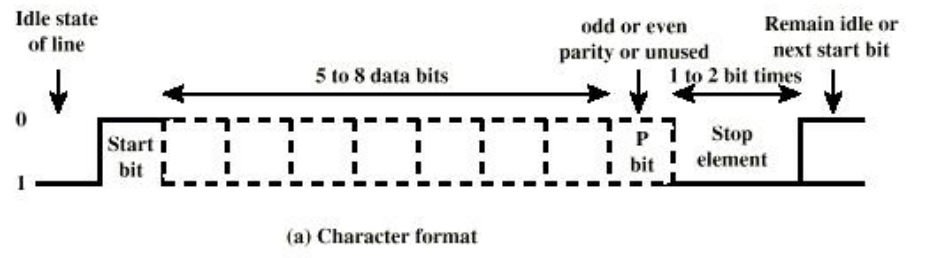
\includegraphics[width=0.86\textwidth]{ch02-async-character.png}
 \caption{异步通信的字符格式。来源：\texttt{Chapter2-物理层.pdf}，PDF第12页（显示页12），局部截取。图中0、1是逻辑状态标注，不能只凭波形画在上方或下方判断其数值。}
 \label{fig:async-character}
\end{figure}

\textbf{计算例：} 若采用1位起始位、8位数据位、1位停止位且不加校验位发送一个字符，总计$1+8+1=10$位；有效数据占$8/10=80\%$，起止附加位占$2/10=20\%$。若再加校验位或使用2位停止位，应把它们计入总位数。

课件列出的优点是实现简单、成本低；代价是每个字符需增加2或3个附加位，课件以约20\%开销概括。它适合短距离、低速率、字符间隔较大的场景，例如键盘输入。实际开销比例取决于数据位、校验位、停止位的配置。

\textbf{同步通信}通常连续传送较大数据块。双方需维持一致的时序，可以使用单独时钟线（适合短距离，且时钟线也可能受损），也可以把时序线索嵌入数据信号或载波中。后文Manchester编码每比特中间都有一次跳变，就可提供时序线索。同步方式减少逐字符起止位开销，但仍可能有同步、组帧或其他开销，不能理解为没有任何附加信息。
\annotationarea[4]

\subsection{模拟通信与数字通信}
课件按信道中传输的信号区分模拟通信与数字通信：传输模拟信号的是模拟通信，传输数字信号的是数字通信。这里判断的是\textbf{信道上实际传输的信号}，不是只看信源原始数据是语音、图像还是比特。例如，模拟语音经过PCM后成为数字信号，可以进入数字通信系统；数字比特也可控制载波，产生连续变化的已调信号。此处的“模拟/数字信号”与“模拟/数字数据”需分开判断。
\annotationarea[4]

\subsection{模拟数据数字化：PCM的三个步骤}
\textbf{脉冲编码调制（PCM）}把模拟数据转换为数字表示。虽然名称中有“调制”，这里讨论的是模拟信源的数字化；它不同于后文用数字数据改变载波的数字调制。
\begin{enumerate}
 \item \textbf{采样：} 在一系列离散时刻读出原信号幅值，使时间离散；幅值此时还可连续取值。
 \item \textbf{量化：} 把幅值映射为预设的有限量化等级，使取值离散。原幅值与代表值之间存在量化误差。
\item \textbf{编码：} 用二进制码表示量化等级。若有$N$级，固定长度编码至少需要$k=\lceil\log_2N\rceil$ bit；若$N=2^k$则正好用$k$ bit。课件简写为$\log_2N$位，对$N$为2的幂次时成立；其他$N$取固定码长时要向上取整。
\end{enumerate}
图\ref{fig:pcm-process}先显示连续波形，再给出3.2、3.9等采样值；量化后成为3、4等等级；最后分别编码为011、100等。图中的脉冲幅度调制（PAM，Pulse Amplitude Modulation）脉冲行表示采样时刻的幅值，下一行体现量化，不可把两行混成同一步。

\begin{figure}[H]
 \centering
 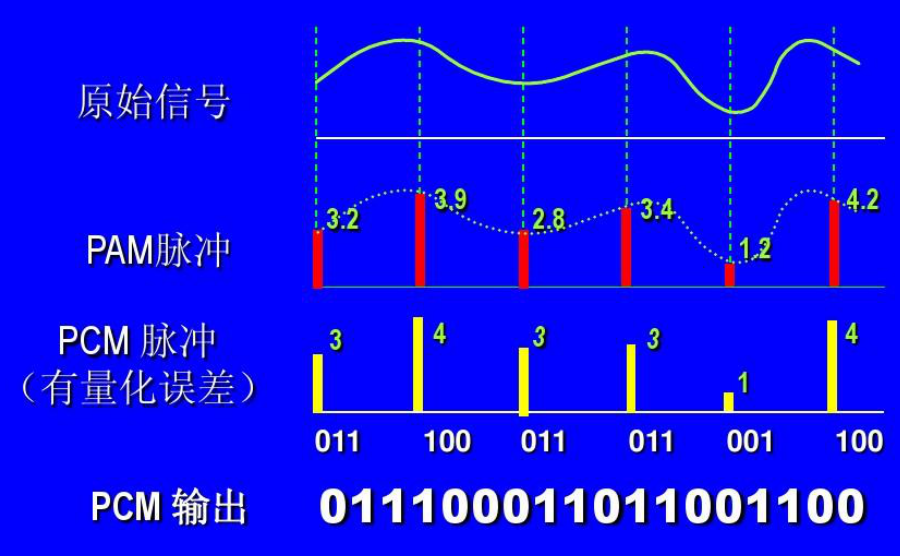
\includegraphics[width=0.78\textwidth]{ch02-pcm-process.png}
 \caption{PCM从连续波形到采样、量化、二进制码的过程。来源：\texttt{Chapter2-物理层.pdf}，PDF第19页（显示页19），局部截取。}
 \label{fig:pcm-process}
\end{figure}

\textbf{课件例题（PDF第19页／显示页19）：} 图中六个采样值依次为3.2、3.9、2.8、3.4、1.2、4.2。按课件的量化格点，它们分别量化为3、4、3、3、1、4；每个等级用3位二进制表示，逐个查码为
\[
3\mapsto011,\quad4\mapsto100,\quad3\mapsto011,\quad3\mapsto011,\quad1\mapsto001,\quad4\mapsto100.
\]
因此输出比特流为$011\ 100\ 011\ 011\ 001\ 100$，去掉分组空格为\texttt{011100011011001100}。量化后的等级可恢复，原采样幅值（例如3.2）不能由码字精确恢复。
\annotationarea[4]

\textbf{参考书补充：采样条件与PCM码率。} 采样过慢时，原来的快速变化可能被误认成较慢的变化，这称为\emph{混叠}。对最高频率为$f_{\max}$的理想带限信号，为避免混叠并重建原信号，通常取$f_s>2f_{\max}$。教材用“不得低于两倍”概括这个条件；$2f_{\max}$是理论边界，等号不能对任意恰好位于带边的信号无条件保证重建。实际设计需要留余量，并先限制输入频带。采样定理不消除随后量化造成的误差。这里限制的是\emph{采样原模拟信号的频率}，不要与后文的无码间串扰码元速率限制混用。若每秒采样$f_s$次、每样本编码$k$ bit，不考虑其他开销，则PCM比特率
\[
 R_{\mathrm{PCM}}=f_sk.
\]
\textbf{自拟例：} 将最高频率3 kHz的带限信号每秒采样8000次，满足$8000>2\times3000$，采用256级量化，则$k=\log_2 256=8$，输出码率$8000\times8=64000$ bit/s，即64 kb/s。这只是数字化后的数据率，不表示一条3 kHz模拟信道可无条件以64 kb/s传输。
\annotationarea[4]

\subsection{扩频：把信息展开到更宽频带}
\textbf{扩频}使承载信息的信号占用比原始数据所需更宽的频带。课件说明可用于模拟或数字数据，并以扩展频带使通信不易被窃听作为用途说明；这不等于加密或保密保证。课件介绍两类：\textbf{跳频}按双方知道的序列在一组载波频率间跳换；\textbf{直接序列扩频}用较长的码片序列表示原来的一比特。接收方依据同样的序列恢复信息。这里“一个信息比特对应多个码片”的想法，也会用于2.5节的码分复用。

课件英文将跳频写作“Frequency hoping”，应为“Frequency hopping”（跳频）。发送端与接收端按共享序列切换频率。

\textbf{学习补充：} 扩频可改善对窄带干扰的抵抗，并可支持不同用户在同一频带工作。它需要相应的同步、编码和接收处理；仅扩展频带不能替代加密。课件还将跳频思想与好莱坞演员Hedy Lamarr联系起来，属于历史备注。

\begin{quote}\small 来源：课件PDF第8--20页（显示页8--20）；教材§2.1.1，PDF第41--42页／印刷第30--31页，§2.1.3的PCM说明，PDF第45页／印刷第34页。对数、PCM码率和80\%效率例是按来源规则补出的基础说明或自拟计算。\end{quote}
\annotationarea[4]

\section{物理介质}
\subsection{导引型介质：信号沿指定通路传播}
导引型介质把信号限制在指定的物理通路中。课件列出架空明线、双绞线、同轴电缆和光纤。

\textbf{架空明线}是架设在空中的裸导线，容易受天气和外界电磁干扰，课件指出其带宽有限。

\textbf{双绞线}由两根绝缘导线相互绞合而成，主要用于基带传输。屏蔽双绞线简称STP（Shielded Twisted Pair），非屏蔽双绞线简称UTP（Unshielded Twisted Pair）。课件给出的UTP类别、频率带宽和典型应用如下：
\begin{center}
\small
\begin{tabularx}{0.97\textwidth}{c c X}
\toprule
类别 & 频率带宽 & 课件列出的典型应用\\
\midrule
3类 & 16 MHz & 低速网络、电话网络\\
4类 & 20 MHz & 10BASE-T以太网\\
5类 & 100 MHz & 10BASE-T以太网、100BASE-T快速以太网\\
超5类（5E） & 100 MHz & 100BASE-T快速以太网、1000BASE-T吉比特以太网\\
6类 & 250 MHz & 1000BASE-T吉比特以太网、ATM网络\\
\bottomrule
\end{tabularx}
\end{center}
表中MHz是线缆频率带宽，不是网络数据率；例如100 MHz不能直接读成100 Mb/s。实际链路速率还取决于接口标准、编码方式、线缆长度等条件。
表中10BASE-T、100BASE-T和1000BASE-T表示相应速率等级的双绞线以太网，后缀T表示双绞线介质；ATM是异步传递模式（Asynchronous Transfer Mode）。

\textbf{同轴电缆}由内导体、绝缘层、外导体屏蔽层和保护套组成，屏蔽结构提高抗干扰能力。课件主要以频带传输举例；\textbf{参考书补充}说明同轴也可用于基带传输，例如早期基带以太网采用50$\,\Omega$电缆，有线电视常用75$\,\Omega$电缆。因此“同轴”描述介质结构，不能独自决定采用基带还是频带技术。

\textbf{光纤}用光导纤维约束并传输光信号。用光线模型理解，纤芯折射率高于包层；当光从纤芯射向包层的入射角满足条件时，光不会折射到包层外，而是在界面反射回纤芯，这称为\textbf{全反射}。光纤不以金属导体中的电流承载数据，因而抗电磁干扰能力强、传输损耗较小、容量潜力大。

光纤分\textbf{多模}和\textbf{单模}。多模允许多种传播模式，传播路径/到达时间的差别会使短光脉冲展宽，限制距离和速率；单模只允许一种传播模式，避免多模间的到达时间差，更适合长距离高速传输。这里的“模”是传播方式，并非信号幅度的“模拟”或数据的“数字”，也不等于“只传一条信息”。教材用直线与反射作示意，本节只用它建立直觉，不把单模定义为光从不受波导约束。

课件在本节点出各介质类别和光纤的基本原理；UTP参数表按课件逐项列出，双绞线、同轴和光纤结构细节则由教材补充。
\annotationarea[4]

\subsection{非导引型介质：自由空间中的传播}
非导引型介质在自由空间中传播电磁波。课件按频率范围列出无线电、红外线、可见光和紫外线等频段及其应用。下表转录课件第24页的频率范围与典型应用；频率范围采用课件给出的近似值。
\begin{center}
\small
\begin{tabularx}{0.97\textwidth}{l l X}
\toprule
频率范围 & 名称 & 课件列出的典型应用\\
\midrule
3--30 Hz & 极低频（ELF） & 远程导航、水下通信\\
30--300 Hz & 超低频（SLF） & 水下通信\\
300--3000 Hz & 特低频（ULF） & 远程导航\\
3--30 kHz & 甚低频（VLF） & 远程导航、水下通信、声纳\\
30--300 kHz & 低频（LF） & 导航、水下通信、无线电信标\\
300--3000 kHz & 中频（MF） & 广播、海事通信、测向、救险、海岸警卫\\
3--30 MHz & 高频（HF） & 远程广播、电报、电话、传真、搜救、飞机与舰船通信\\
30--300 MHz & 甚高频（VHF） & 电视、调频广播、陆地交通、空中交通管制、导航、飞机通信\\
0.3--3 GHz & 特高频（UHF） & 电视、蜂窝网、微波链路、导航、卫星通信、全球定位系统（GPS）、监视雷达\\
3--30 GHz & 超高频（SHF） & 卫星通信、微波链路、机载雷达、气象雷达、公用陆地移动通信\\
30--300 GHz & 极高频（EHF） & 雷达着陆系统、卫星通信、移动通信、铁路业务\\
300 GHz--3 THz & 亚毫米波（0.1--1 mm） & 课件列为尚未划分、实验应用\\
43--430 THz & 红外线（7--0.7 $\mu$m） & 光通信系统\\
430--750 THz & 可见光（0.7--0.4 $\mu$m） & 光通信系统\\
750--3000 THz & 紫外线（0.4--0.1 $\mu$m） & 光通信系统\\
\bottomrule
\end{tabularx}
\end{center}

传播途径方面，课件分为：
\begin{itemize}
 \item \textbf{地波传播：} 约2 MHz以下的电磁波趋向沿地球表面传播，具有一定绕射能力；低频和甚低频地波可传播数百米到数千公里。
 \item \textbf{天波传播：} 电离层约在地表上方60--400 km。课件以约2--30 MHz为例，说明这一区间的电磁波可受电离层反射回地面，传播距离可超过10000 km。电离层密度和厚度随时间变化，因此课件把这种信道列为随参信道。
 \item \textbf{视线传播：} 课件指出频率高于30 MHz的电磁波通常穿透电离层，地面绕射能力较弱，因此多采用无遮挡的点对点直线传播；可用地面中继站或卫星中继站接力。
\end{itemize}
这些传播方式是课件介绍的典型情况；实际无线链路还受环境、天线和具体频率影响。

\textbf{补充说明：} 若视线链路被山体或建筑物遮挡，需要调整站点或设置中继；单纯提高比特率不能消除传播路径上的遮挡。

\begin{quote}\small 来源：课件PDF第21--26页（显示页21--26）；教材§2.2.1，PDF第53--55页／印刷第42--44页。单模/多模解释补全了教材几何示意中的适用边界。\end{quote}
\annotationarea[4]

\section{信道与信道容量}\label{sec:channel-capacity}
\subsection{模型与限制：为何不能任意提高速率}
\textbf{狭义信道}指传输介质；\textbf{广义信道}还包括发送/接收变换设备、天线、调制器等。\textbf{恒参信道}的主要参数在研究时段内可近似不变；\textbf{随参信道}的衰减和时延会随时间改变，并可能有多径传播。多径是同一信号沿不同路径到达接收端，各路径时延不同，接收信号会相互叠加。

课件列举的有线信道、微波视线链路和卫星链路通常可按恒参信道分析。理想恒参信道不失真；实际恒参信道会对信号产生固定衰减和固定时延。许多无线信道是随参信道，衰减和时延会随机变化，且可能出现多径传播。

要提高比特率，可以缩短码元时间，也可以让每码元有更多状态；但两条路都有限制。带宽有限会改变波形，发送太密时相邻码元可能相互影响，这叫\textbf{码间串扰}。噪声则会扰动接收信号，让过于相近的状态难以区分。课件的两个公式分别说明带宽限制与噪声限制。

\textbf{信道容量}描述给定信道模型下可可靠传输的信息速率上限。课件用“无差错的最大平均速率”概括；对有噪声的香农模型，更准确地说，在低于容量的速率下，理论上可用合适编码把错误概率降得任意小。容量是理论限制，不是设备实际吞吐量的承诺。
\annotationarea[4]

\subsection{奈奎斯特：带宽限制一码元要占多久}
\textbf{条件：} 课件和教材采用理想、带限、无噪声的低通信道模型；频率带宽为$B$ Hz，使用$M$种可区分码元状态。满足无码间串扰条件时，极限码元速率为$2B$ Baud，因此
\[
 R_B\leq2B,\qquad C_N=2B\log_2M\quad\text{b/s}.
\]
公式里的2不是“一个比特要发两次”；它来自该信道模型的无码间串扰条件。$2B$回答每秒最多安排多少码元，$\log_2M$回答每码元携带多少比特，两者相乘得到比特率上界。

\textbf{课件例题（PDF第30页／显示页30）：} 无噪声链路带宽为3 kHz，采用4个相位、每个相位有4种幅度的QAM方案。题目已说明每种组合都是可区分状态，所以
\begin{enumerate}
 \item 数状态：$M=4\times4=16$，每码元携带$\log_2 16=4$ bit。
 \item 换单位：$B=3\times10^3$ Hz；最大码元速率$2B=6000$ Baud。
 \item 求数据率：$C_N=6000\times4=24000$ b/s，即24 kb/s。
\end{enumerate}
增加$M$可在同一码元速率下携带更多比特；无噪声模型并不因此给实际含噪线路提供无限速率。
\annotationarea[4]

\subsection{香农：噪声使信号状态不能无限靠近}
\textbf{条件：} 带限的加性高斯白噪声信道模型；$B$是频率带宽（Hz），$S$、$N$分别是接收处信号和噪声的平均功率，以相同单位计量。记线性信噪比$\gamma=S/N$，它无单位，则
\[
 C_S=B\log_2(1+\gamma)\quad\text{b/s}.
\]
$\gamma$越大，信号越容易与噪声区分；$B$越大，能使用的频带越宽。对固定$B$与$\gamma$，换调制方案本身不能突破这个容量；该式也没有给出实现容量所需的具体编码算法。

课件第31页在文字定义中称$S/N$为“信号能量与噪声能量之比”，随后分贝公式写为“信号功率/噪声功率”。为与香农公式的常用写法和教材一致，本笔记将$S$、$N$按同一接收条件下的平均功率解释；若在相同观察时长内取能量比，数值比值相同。\textbf{分贝（dB，decibel）怎样换算？} 信噪比也可用分贝值$\gamma_{\mathrm{dB}}$表示：
\[
 \gamma_{\mathrm{dB}}=10\log_{10}\gamma,
 \qquad \gamma=10^{\gamma_{\mathrm{dB}}/10}.
\]
$\log_{10}$问的是“10的几次方等于该数”，与上面的$\log_2$底数不同。10 dB对应10倍，20 dB对应100倍，30 dB对应1000倍。代入香农式的是\textbf{线性比值}，不能直接把30 dB当成30代进去。

\textbf{课件例题（PDF第31页／显示页31）：} $B=2$ MHz，信噪比30 dB。
\begin{enumerate}
 \item 换回线性比值：$\gamma=10^{30/10}=1000$。
 \item 换带宽单位：$B=2\times10^6$ Hz。
 \item 代入：$C_S=2\times10^6\log_2(1001)\approx19.93\times10^6$ b/s，约20 Mb/s。因为$2^{10}=1024$接近1001，$\log_2(1001)$可近似为10。
\end{enumerate}
若题目直接给$S=0.14$ W、$N=0.02$ W，则$\gamma=7$，无须先变成dB再变回来。
\annotationarea[4]

\subsection{两个上界怎样一起用}
若题目同时给出$B$、$M$和信噪比，在上述公式均适用的课内模型中，应分别计算两种限制：
\[
 R_b\leq\min\{2B\log_2M,\ B\log_2(1+\gamma)\}.
\]
这给出共同上界；实际系统是否能达到它，还取决于具体波形、编码、设备和开销，不能把“上界”自动解释成实际吞吐量。

\textbf{参考书代表例（§2.1.4第12题，PDF第47页／印刷第36页；解析PDF第50页／印刷第39页）：} 4 kHz信道传输两状态的二进制信号，线性信噪比127。
\begin{enumerate}
 \item 噪声上界：$C_S=4000\log_2(128)=28000$ b/s。
 \item 题目同时限定$M=2$：$C_N=2\times4000\times\log_2 2=8000$ b/s。
 \item 按课内两个限制取较小上界，为8 kb/s。28 kb/s忽略了两状态限制。
\end{enumerate}
\textbf{计算前自查：} 带宽单位是否Hz？题目给的是线性比值还是dB？$M$是所有可区分状态的总数吗？求的是波特率、容量上限，还是已给定的实际比特率？

\begin{quote}\small 来源：课件PDF第27--31页（显示页27--31）；教材§2.1.2，PDF第42--43页／印刷第31--32页；联合限制解析见PDF第50--51页／印刷第39--40页。奈氏式的使用沿课件与教材的低通模型；不把该式无条件推广到任意带通信道。\end{quote}
\annotationarea[4]

\section{信道共享：多路复用}
\subsection{复用与分用：几路数据共用一条通路}
\textbf{多路复用（multiplexing）}把链路或网络资源（如频率带宽、时间、波长或码）划分为资源片，再分配给多个通信用户。发送端用\textbf{复用器}把各路信号组合到共享通路；接收端用\textbf{分用器}按对应规则分离。课件指出，用户占用的资源片在没有数据时可能闲置；复用的作用是安排共享方式，不会凭空增加信道容量。
\annotationarea[4]

\subsection{FDM、TDM和WDM}
\textbf{频分复用（FDM）}把信道的频率带宽划成多个不同频带，用户在通信期间持续占用各自频带，因此可以同时传输。课件第36页特别说明，这里的带宽是Hz计量的频率带宽，不是bit/s计量的数据率；没有数据时，分配给该用户的频带可能空闲。\textbf{课件笔误：}第36页标题将缩写写成“FMD”，正文图中写作“FDM”；本笔记统一使用正确缩写FDM。

\begin{figure}[H]
 \centering
 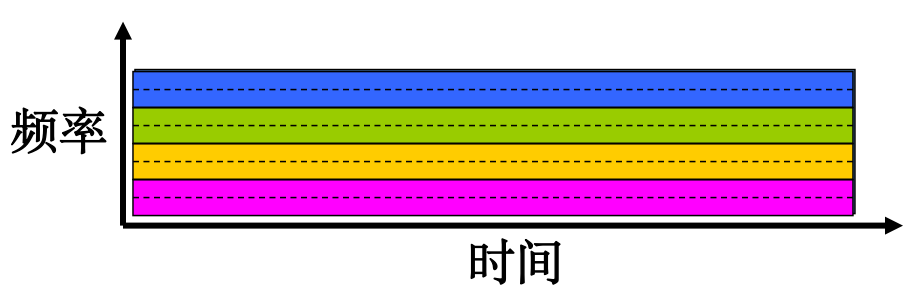
\includegraphics[width=0.74\textwidth]{ch02-fdm.png}
 \caption{FDM把同一时间的信号安排在不同频率带内。来源：\texttt{Chapter2-物理层.pdf}，PDF第36页（显示页36），局部截取。}
 \label{fig:fdm}
\end{figure}
图中纵轴为频率、横轴为时间，四条水平色带表示四个用户分别占用的频率范围；每条带在整个时间方向持续存在。

\textbf{时分复用（TDM）}把时间划成重复出现的TDM帧，每帧再分固定时隙，各用户在各自时隙使用该通路。图\ref{fig:tdm}中的A、B、C、D不是四个不同频带，而是在同一频带上依次获得发送时间；A的时隙每帧重复一次。

\begin{figure}[H]
 \centering
 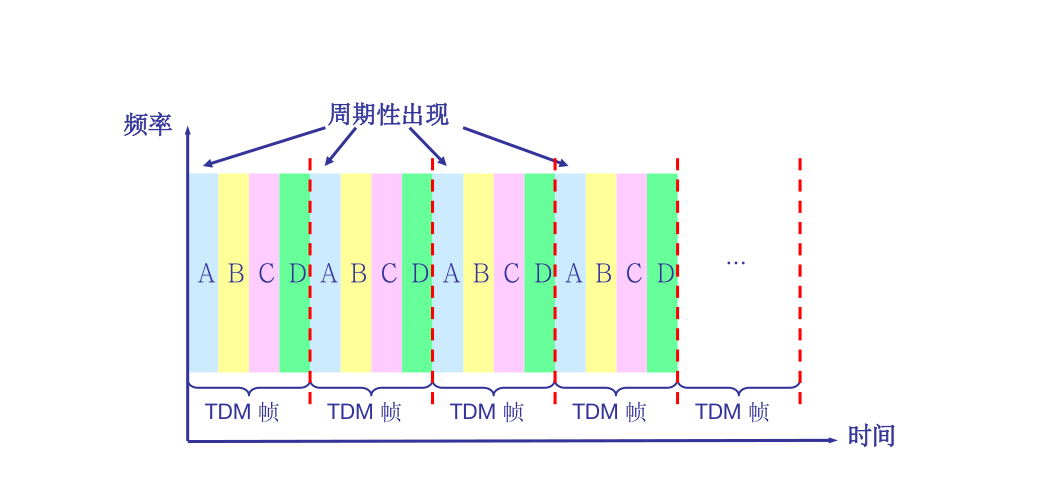
\includegraphics[width=0.82\textwidth]{ch02-tdm.png}
 \caption{TDM帧中的固定时隙周期性重复。来源：\texttt{Chapter2-物理层.pdf}，PDF第38页（显示页38），局部截取。}
 \label{fig:tdm}
\end{figure}

课件图中一个TDM帧包含A、B、C、D四个固定时隙，后续帧按同样次序重复；同一用户的时隙周期性出现。各用户在不同时间使用相同频带。这里的TDM帧是信道时间的周期单位，不是数据链路层的数据帧。固定分配的时隙即使暂时没有数据，也可能闲置。

\textbf{波分复用（WDM）}用不同光波长在同一根光纤上传输。波长与频率对应，故课件把WDM理解为光的频分复用。课件第40页中8路各2.5 Gb/s合成20 Gb/s，是各路数据率相加的例子；前提是共享光纤系统能容纳这些波长通道，并忽略额外开销。

\begin{figure}[H]
 \centering
 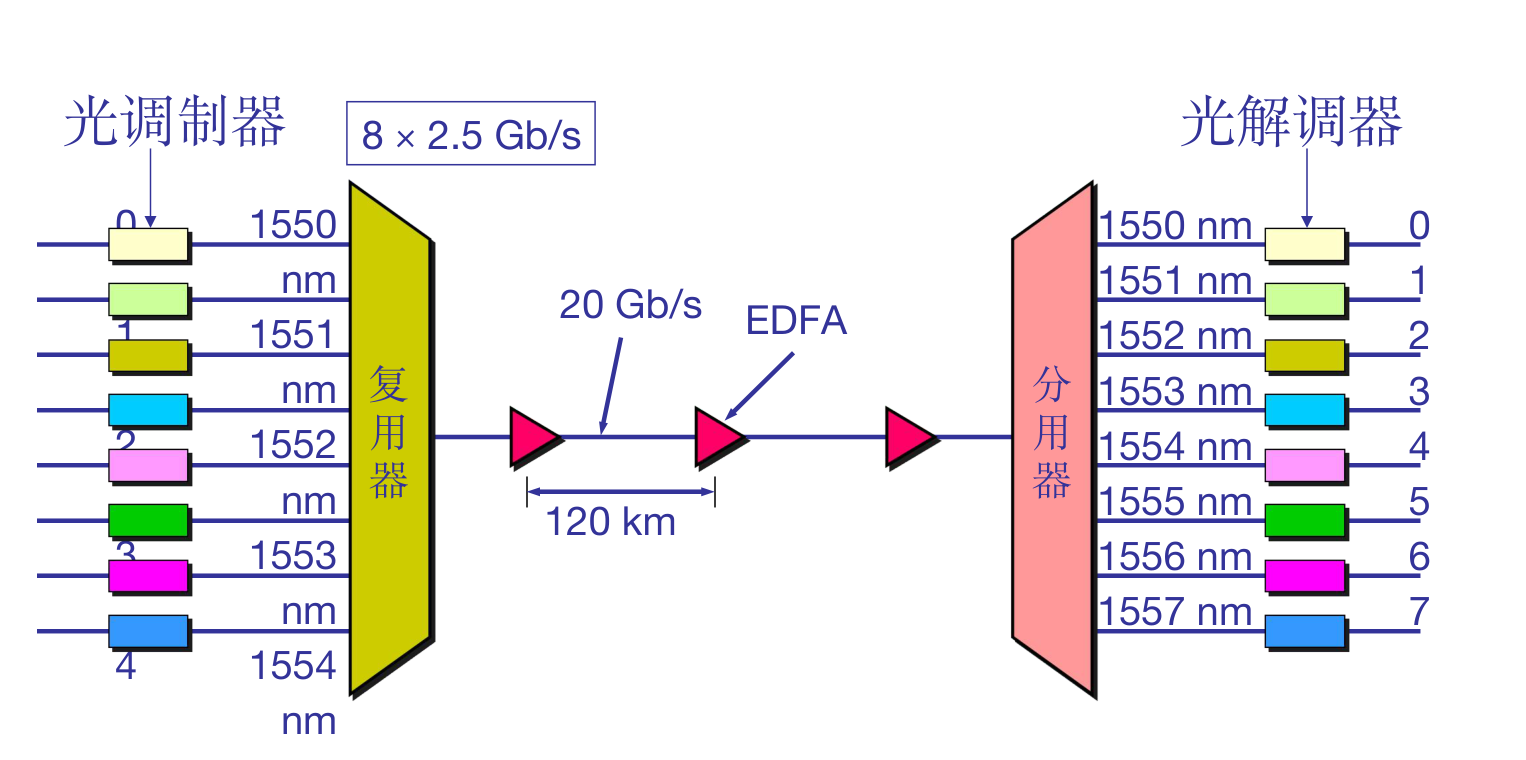
\includegraphics[width=0.92\textwidth]{ch02-wdm.png}
 \caption{WDM用不同波长承载多路光信号，并在接收端分离。来源：\texttt{Chapter2-物理层.pdf}，PDF第40页（显示页40），局部截取。}
 \label{fig:wdm}
\end{figure}
图中8个通道分别使用1550--1557 nm波长，复用器把各波长的光信号合到一根光纤，接收端分用器再分开；EDFA为掺铒光纤放大器，课件标注光纤段约120 km。计算总数据率时，$8\times2.5=20$ Gb/s。
\annotationarea[4]

\subsection{CDM：靠正交码片分离同频用户}
\textbf{码分复用（CDM）}给用户分配不同码片序列，让用户在同一频带、同一时间发送。一个信息比特展开成$m$个\textbf{码片}；每码片在理想数学模型中取$+1$或$-1$。用$d_i=+1$表示信息比特1，用$d_i=-1$表示信息比特0；未发送时记$d_i=0$。

用户$i$的码片向量记为$S_i$。发送1时发送$S_i$，发送0时发送$-S_i$，也就是把每个码片正负反转。接收端看到各用户信号的叠加：
\[
 P=\sum_i d_iS_i.
\]
这个式子只要求同一位置相加。两用户在某位置都发送$+1$，叠加值就为2；一正一负则为0，所以合成信号不必仍只有$\pm1$。

\textbf{内积是什么？} 两个等长向量的内积就是对应元素相乘，再将结果相加，例如$(1,-1)\cdot(1,1)=1-1=0$。两个码片序列内积为0，称它们\textbf{正交}。课件要求不同用户的码片码相互正交，而同一码的自内积为$m$，因此可用
\[
 d_i=\frac{S_i\cdot P}{m}
\]
恢复用户$i$的数据：别人的码与$S_i$点乘为0被消去，自己的码产生$m$倍，除以$m$回到原值。

\textbf{课件示例码片序列（PDF第41页／显示页41）：} 课件给出的一个用户码为
\[
S=(-1,-1,-1,+1,+1,-1,+1,+1).
\]
若码片长度为$m$，同一用户码的自内积为$S_i\cdot S_i=m$；不同用户码两两正交，即$i\ne j$时$S_i\cdot S_j=0$。

\textbf{课件编解码例题（PDF第43--44页／显示页43--44）：} 图\ref{fig:cdm-example}给出用户1、用户2的码片与两个时隙的数据。按图中码片顺序读取，
\[
 S_1=(1,1,1,-1,1,-1,-1,-1),\qquad
 S_2=(1,-1,1,1,1,1,-1,1),\qquad m=8.
\]
为避免下标混淆，记$b_{u,t}$为用户$u$在时隙$t$发送的数据值；$+1$表示比特1，$-1$表示比特0。课件图中用户1在时隙1发送0、时隙0发送1，用户2在两个时隙都发送1，即$b_{1,1}=-1$、$b_{1,0}=+1$、$b_{2,1}=+1$、$b_{2,0}=+1$。
先核对正交：
\[
S_1\cdot S_2=1-1+1-1+1-1+1-1=0.
\]
时隙1的信道输出是两个编码序列逐项相加：
\[
P_1=b_{1,1}S_1+b_{2,1}S_2=-S_1+S_2=(0,-2,0,2,0,2,0,2).
\]
时隙0中两个用户都发送1，因此
\[
P_0=b_{1,0}S_1+b_{2,0}S_2=S_1+S_2=(2,0,2,0,2,0,-2,0).
\]
对每个接收用户，用$\hat b_{u,t}=(S_u\cdot P_t)/8$解码。时隙1：$S_1\cdot P_1=-8$，故用户1数据为$-1$（比特0）；$S_2\cdot P_1=8$，故用户2数据为$+1$（比特1）。时隙0：$S_1\cdot P_0=8$且$S_2\cdot P_0=8$，两用户均解得$+1$（比特1）。

\begin{figure}[H]
 \centering
 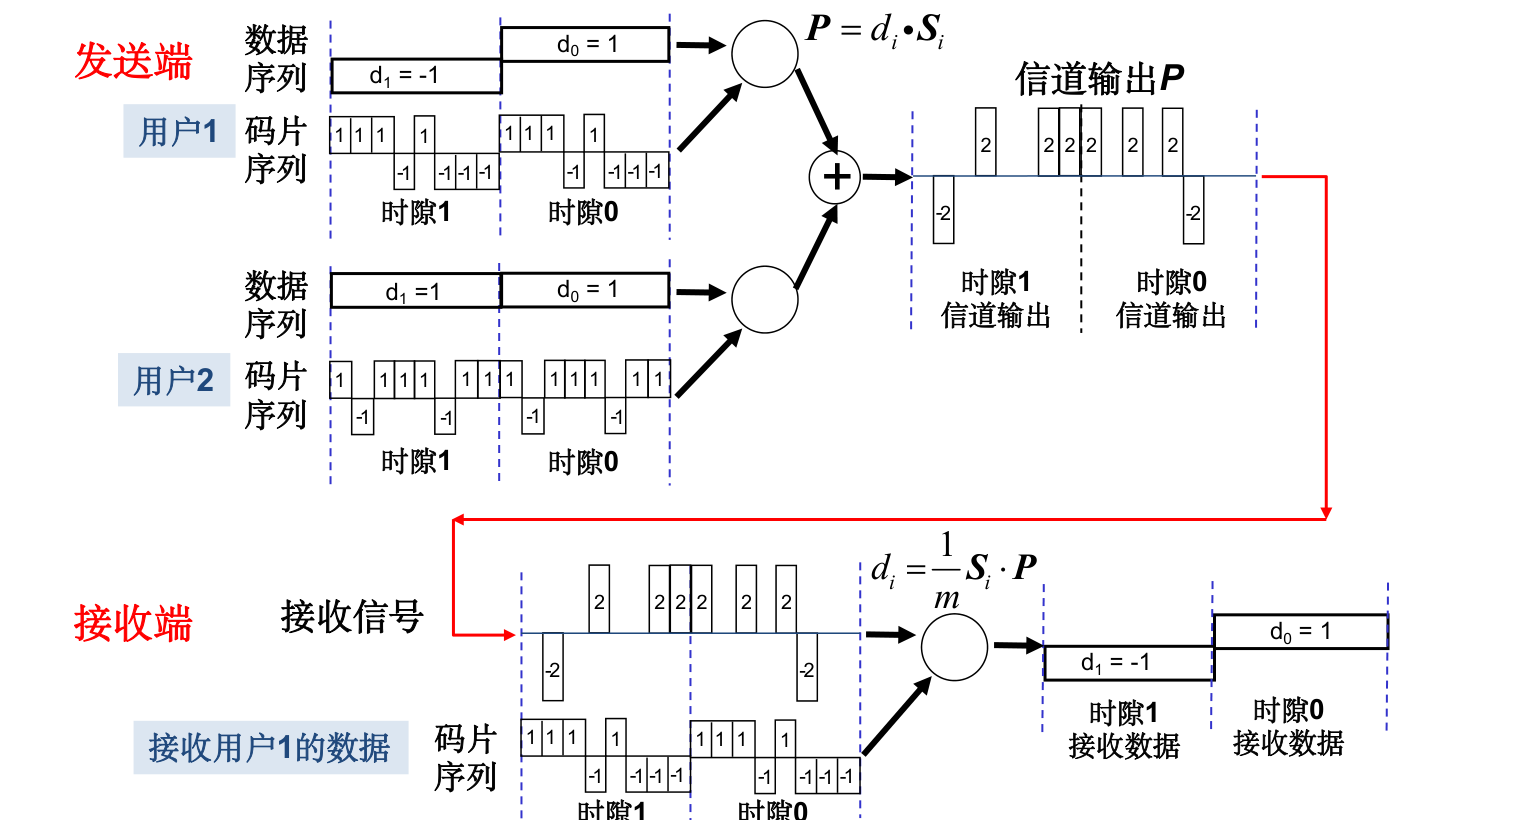
\includegraphics[width=0.96\textwidth]{ch02-cdm-example.png}
 \caption{课件CDM双用户双时隙编解码例。来源：\texttt{Chapter2-物理层.pdf}，PDF第44页（显示页44），局部截取。}
 \label{fig:cdm-example}
\end{figure}
\textbf{适用条件与易错点。} 以上是码片对齐、理想正交、按相同幅度归一且无噪声的模型；实际接收结果会受到噪声、不同功率、时延和多径影响。理想模型中的解码值0表示该用户未发送，\textbf{不表示它发送了信息比特0}。码片也不是原始信息比特：每信息比特展开$m$码片时，码片速率为信息比特率的$m$倍。

\begin{quote}\small 来源：课件PDF第32--44页（显示页32--44）；FDM图取第36页，TDM图取第38页，WDM图取第40页，CDM例图取第44页，均为局部截取。教材第2章没有按这一结构集中讲复用，本节定义、编码与解码以课件为直接依据。\end{quote}
\annotationarea[4]

\section{基带传输}\label{sec:baseband}
\subsection{直接传送基带信号与线路编码}
\textbf{基带信号}是未经搬移到载波频带的原始信号，往往含较多低频甚至直流成分。\textbf{基带传输}是在信道中直接传输基带信号；数字基带传输先把比特映射为适合线路的电平或跳变，再直接发送。这里的\textbf{线路编码}规定“0和1在波形上怎样表现”，不等同于PCM的样本数字化，也不等同于压缩文件。

基带通常适合具有低通特性的有线通路；信号在途中可能衰减、畸变或受噪声影响。选择码型时既要让接收方区分0、1，还要考虑同步信息、直流分量及占用带宽。以下规则按课件约定，遇到采用相反0/1定义的题目应先读其约定。
\annotationarea[4]

\subsection{NRZ、RZ、差分码与AMI}
\textbf{不归零码（NRZ）}在一个比特区间内保持相应电平，区间中途不强制回零。课件的\emph{单极NRZ}用$+E$表示1、0电平表示0；\emph{双极NRZ}用正负电平表示两种比特。这里单极/双极描述使用的电平，归零/不归零描述区间内是否回零，二者是不同分类维度。

\begin{figure}[H]
 \centering
 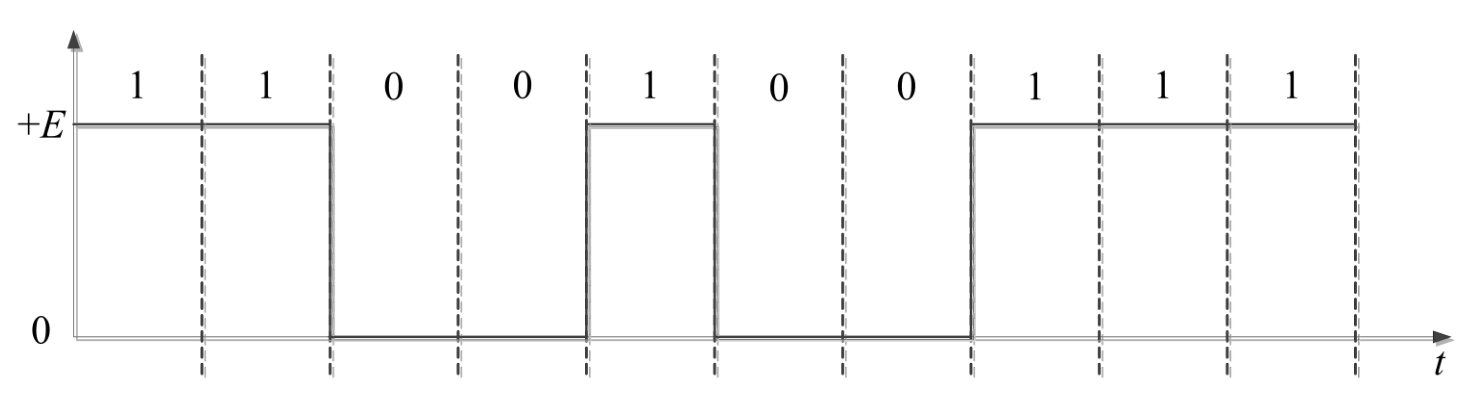
\includegraphics[width=0.85\textwidth]{ch02-nrz-wave.png}
 \caption{单极NRZ：连续相同比特可没有边界跳变。来源：\texttt{Chapter2-物理层.pdf}，PDF第48页（显示页48），波形局部截取。}
 \label{fig:nrz-wave}
\end{figure}

图\ref{fig:nrz-wave}中顶部数字给出每个比特的值，虚线划分区间。连续两个1保持同一电平，连续三个0也是如此；若没有额外时序线索，只观察这段平直线不能知道它跨了几个比特。NRZ本身不保证自同步，实际系统需要另设同步机制。

课件第49页的双极NRZ用$+E$和$-E$分别表示两种比特。课件图的共同输入序列为$1100100111$：单极NRZ输出电平依次为$+E,+E,0,0,+E,0,0,+E,+E,+E$；双极NRZ按“1为$+E$、0为$-E$”的图示约定，输出为$+E,+E,-E,-E,+E,-E,-E,+E,+E,+E$。

\textbf{归零码（RZ）}在每比特的部分时段保持相应非零脉冲，随后回到零。课件单极RZ用正脉冲表示1、全程零表示0；双极RZ用正/负脉冲分别表示两种比特并都回零。占空比是一个区间内非零脉冲占据的时间比例，可写为$D=T_{\mathrm{nz}}/T_b$，其中$T_{\mathrm{nz}}$为非零脉冲时长、$T_b$为一个码元周期。图\ref{fig:rz-wave}中1的脉冲持续$T_b/2$，所以占空比为50\%。

\begin{figure}[H]
 \centering
 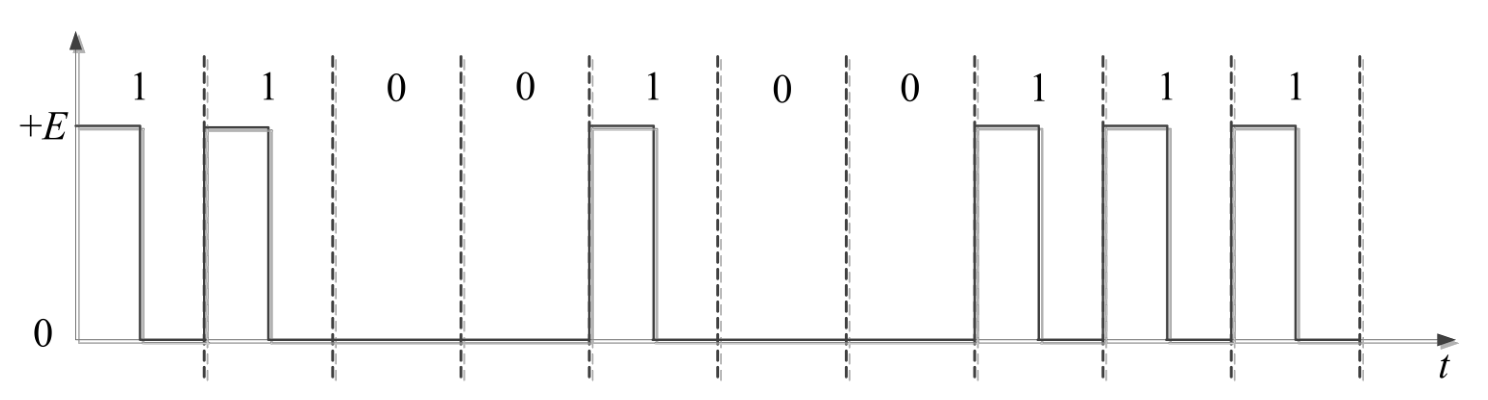
\includegraphics[width=0.85\textwidth]{ch02-rz-wave.png}
 \caption{单极RZ：1的脉冲中途归零，0仍为零电平。来源：\texttt{Chapter2-物理层.pdf}，PDF第50页（显示页50），波形局部截取。}
 \label{fig:rz-wave}
\end{figure}

回零增加电平变化，通常增加对频率带宽的要求。\textbf{单极RZ遇长串0仍没有跳变，不能保证所有比特序列都有同步线索}；双极RZ每比特有非零脉冲并回零，提供的时序线索不同。不能只看到RZ名称就断言“一定自同步”。

课件第51页的双极RZ在比特区间前半段用$+E$表示1、$-E$表示0，后半段都回到零；它与双极NRZ的区别是码元中途是否回零。

\textbf{差分码（相对码）}用相邻码元之间是否发生电平变化表达信息。课件第52页约定“发生跳变表示1、不跳变表示0”。课件波形输入为$1100100111$；以图示的首个电平$+E$为初始状态，首位之后每遇到1就在$0$与$+E$之间翻转，遇到0就保持，输出电平依次为$+E,0,0,0,+E,+E,+E,0,+E,0$。教材介绍的NRZI采用“起始跳变表示0、不变表示1”的常见另一约定。遇到具体题目要按题目给出的0/1约定和初始状态编码。
\annotationarea[4]

\textbf{AMI（Alternative Mark Inversion，信号交替反转码）}把0编码成零电平，依次出现的1交替编码成$+E$、$-E$。课件第53页图中AMI传输码元序列为$+1,0,0,0,0,-1,0,0,0,0,+1,-1,0,0,0,0,+1,-1$；按“0为零电平、正负脉冲都代表信息位1”解码，信息位为$100001000011000011$。长串0仍没有跳变。
\annotationarea[4]

\subsection{Manchester与差分Manchester：每位都有同步跳变}
\textbf{Manchester编码}把一个比特时间分为两半，中间必须跳变。按课件第54页：高到低表示1，低到高表示0。中点的跳变既标示时序，又用方向表示数据；比特边界是否跳变由相邻数据决定，不能把边界跳变误当成中点规则。

\textbf{差分Manchester编码}也在每比特中点跳变，但中点只用于同步；数据由比特\emph{开始处}是否跳变表示。按课件第55页：起始跳变表示0，起始不跳变表示1。它与课件第52页的普通差分码相比，多了每比特中点的固定跳变，规则也不同。

\begin{figure}[H]
 \centering
 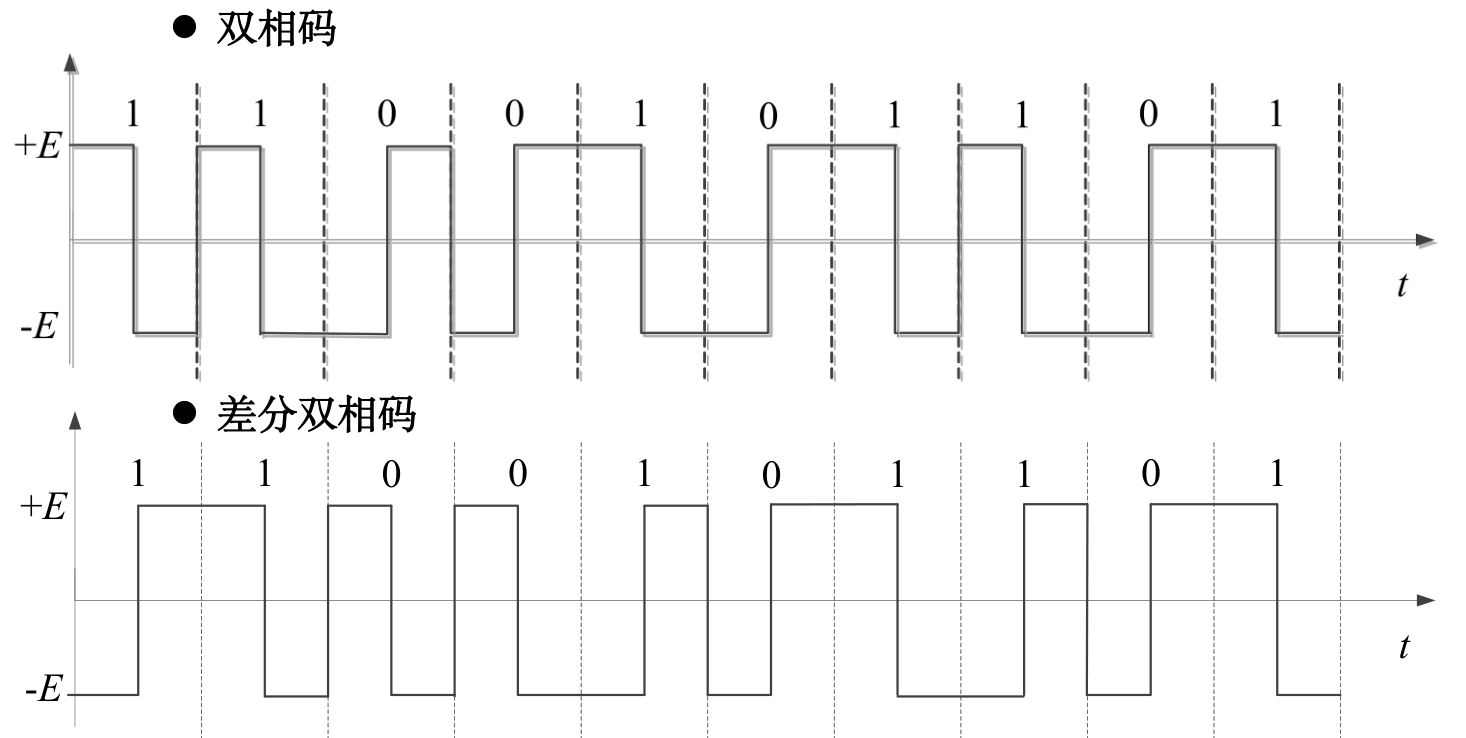
\includegraphics[width=0.93\textwidth]{ch02-line-codes.png}
 \caption{上：Manchester；下：差分Manchester。来源：\texttt{Chapter2-物理层.pdf}，PDF第56页（显示页56），波形局部截取。}
 \label{fig:line-codes}
\end{figure}

\textbf{读图方法。} 先用顶部0/1及竖线定位每比特区间，再看区间中点跳变；对下图还需看每比特起点，第一位的起点要依已知初始参考电平判断。上下图的中点跳变都服务同步，但只有上图按中点方向读数据。

\textbf{课件例题（PDF第56页／显示页56）：} 输入比特为$1100101101$。按课件给定的Manchester约定逐位编码：
\begin{center}
\begin{tabular}{lcccccccccc}
\toprule
输入比特 & 1 & 1 & 0 & 0 & 1 & 0 & 1 & 1 & 0 & 1\\
\midrule
Manchester & HL & HL & LH & LH & HL & LH & HL & HL & LH & HL\\
差分Manchester & LH & HL & HL & HL & LH & LH & HL & LH & LH & HL\\
\bottomrule
\end{tabular}
\end{center}
表中H、L分别表示高、低电平；例如HL表示一个比特前半周期为高、后半周期为低。Manchester每个比特中点都跳变，H到L表示1、L到H表示0。差分Manchester每个中点也跳变，中点只用于同步；比特起点跳变表示0、不跳变表示1。按课件图示，首位开始前的参考电平为L；逐位依据前一位终点和当前比特计算，得到表中的差分Manchester波形。初始参考电平不同会使整条波形整体反相，但相对变化规则不变。
\annotationarea[4]

两种编码都通过固定中点跳变提高时钟恢复能力，代价是同一比特率下更多电平变化、通常需要更宽带宽。课件称用两个脉冲编码一比特；这不表示有效数据比特率被算作原来的两倍。10 Mb/s传统以太网采用Manchester，是后文Ethernet的基础。
\annotationarea[4]

\subsection{nBmB：用冗余码组改善线路特性}
\textbf{nBmB编码}把$n$位数据映射为$m$位新码组，其中$m>n$。$2^n$种数据组合从$2^m$个码组中选择合适表示，使线路上更容易出现需要的跳变等特性。冗余还可留出控制、保留或无效码组；出现无效组可提示差错，但不是所有差错都能检出。

课件以\textbf{4B5B}为例：4位数据有16种组合，5位线路码有32种组合，从中选16种代表数据，其余可承担其他用途或禁用。\textbf{课件表述修正：} 第57页将余下16种一概称作“禁用码”，实际应区分控制码、保留码和无效码，不能把任意非数据码都认作传输出错。

\textbf{自拟计算：} 输入数据率100 Mb/s，经4B5B映射且不计其他开销，线路码比特率为$100\times5/4=125$ Mb/s；数据占线路码的$4/5=80\%$，线路位数比输入增加25\%。4B5B是分组映射，常还需配合具体线路波形编码；它本身不是“用五种电压发送四比特”。课件列出的100BASE-TX/FX是使用该映射的实例，不推广为所有快速以太网都相同。
\annotationarea[4]

\begin{quote}\small 来源：课件PDF第45--57页（显示页45--57）；教材§2.1.3，PDF第44--45页／印刷第33--34页。本节显式区分课件差分码与教材NRZI的0/1约定，并补全单极RZ长0与4B5B余码的边界。\end{quote}
\annotationarea[4]

\section{频带传输}\label{sec:passband}
\subsection{载波、幅度、频率与相位}
许多信道适合通过一段离开零频的频带，而不能直接通过所需基带波形。\textbf{频带传输}让基带数据控制载波的某些参数，把信息放到适合信道的频带上；接收端再作解调。频带传输不是“发送更多频率就一定更快”，而是适配信道的传输技术。

载波常写成
\[
 s(t)=A\cos(2\pi ft+\phi).
\]
$A$是振幅，表示波形离中心线的最大幅度；$f$是频率（Hz），表示每秒振荡多少周期；$\phi$是相位，决定某时刻处于周期中的哪一位置。一个周期为$2\pi$弧度，$\pi$是半周期、$\pi/2$是四分之一周期。\textbf{学习补充：} 相位差$\pi$的两条同频同幅余弦波，在同一时刻的取值符号相反；相位差不是频率不同。

课件把模拟基带控制载波称模拟调制，把数字基带控制载波称数字调制。本节集中学习后者。数字调制中的载波仍是连续波形；比特体现在对载波状态的有限种选择中。
\annotationarea[4]

\subsection{二进制调制：每码元两种状态}
\textbf{2ASK（幅移键控）}用两种振幅表示0和1。课件的开关键控示例以有载波表示1、无载波表示0；图\ref{fig:ask-wave}从上到下是数字基带、未调制载波、输出波形。基带为0时输出消失，基带为1时出现振荡。

\begin{figure}[H]
 \centering
 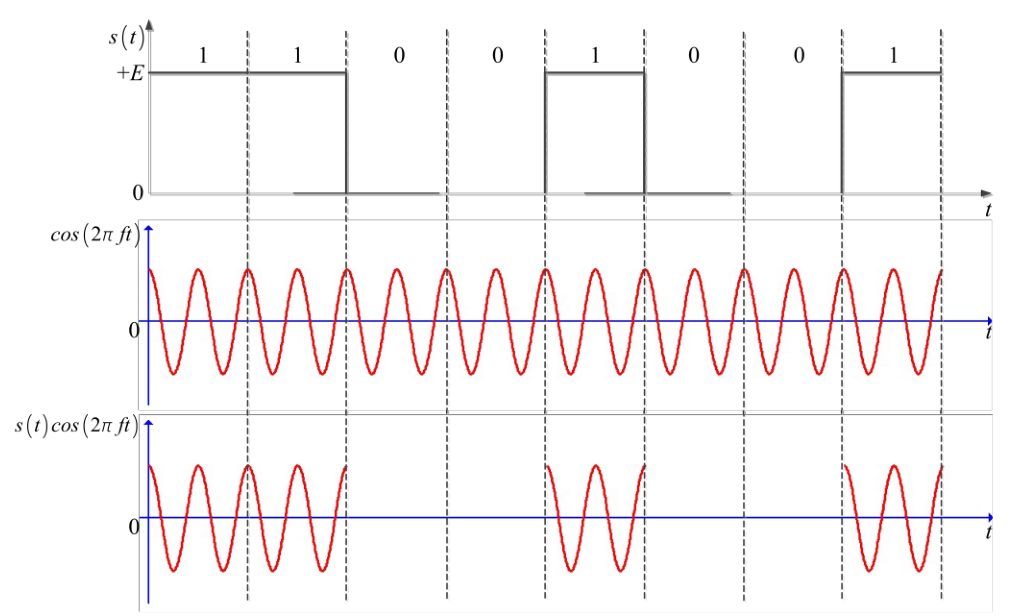
\includegraphics[width=0.69\textwidth]{ch02-ask-wave.png}
 \caption{2ASK通过是否保留载波幅度表达比特。来源：\texttt{Chapter2-物理层.pdf}，PDF第61页（显示页61），波形局部截取。}
 \label{fig:ask-wave}
\end{figure}
课件例图的输入为$11001001$，所以2ASK输出依次为“有载波、有载波、无载波、无载波、有载波、无载波、无载波、有载波”。这里用有无载波表示两种状态。课件的表达式为$y(t)=s(t)\cos(2\pi ft)$，其中$s(t)$是单极数字基带信号，$f$为载波频率；基带为0时幅度为0，基带为1时保留载波。
\annotationarea[4]

\textbf{2FSK（频移键控）}用两个不同频率$f_1$、$f_2$表示0、1，课件第62页约定0用$f_1$、1用$f_2$。图\ref{fig:fsk-wave}中不同码元区间的振荡疏密不同，疏密反映频率，而不只是幅度变化。

\begin{figure}[H]
 \centering
 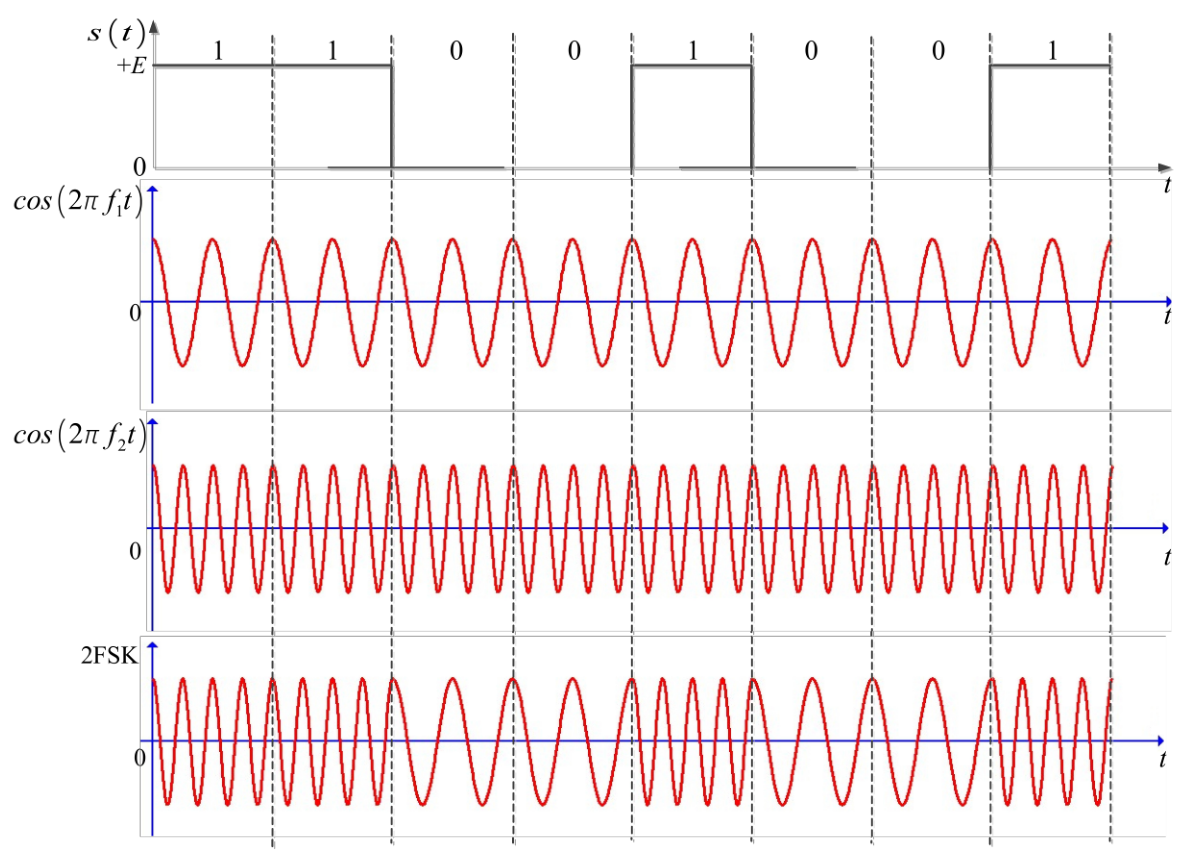
\includegraphics[width=0.69\textwidth]{ch02-fsk-wave.png}
 \caption{2FSK在两种载波频率中选择。来源：\texttt{Chapter2-物理层.pdf}，PDF第63页（显示页63），波形局部截取。}
 \label{fig:fsk-wave}
\end{figure}
课件例图输入仍为$11001001$；逐位替换为载波频率后，输出频率顺序为$f_2,f_2,f_1,f_1,f_2,f_1,f_1,f_2$。在第$n$个码元区间，课件约定$y(t)=\cos(2\pi f_1t)$表示0、$y(t)=\cos(2\pi f_2t)$表示1；$f_1$、$f_2$是两种不同载波频率。
\annotationarea[4]

\textbf{2PSK（相移键控）}用两种绝对相位表示比特，课件第64页以$\phi_0$表示0、$\phi_0+\pi$表示1。一个码元内可写为$y(t)=\cos(2\pi ft+\phi_n)$，其中$\phi_n=\phi_0$对应0、$\phi_n=\phi_0+\pi$对应1。绝对相位的判断需要接收方有相位参考。图\ref{fig:psk-wave}采用$\phi_0=-\pi/2$作示例，重点看相位对应关系，不必把该初始值背成所有系统的固定值。

\begin{figure}[H]
 \centering
 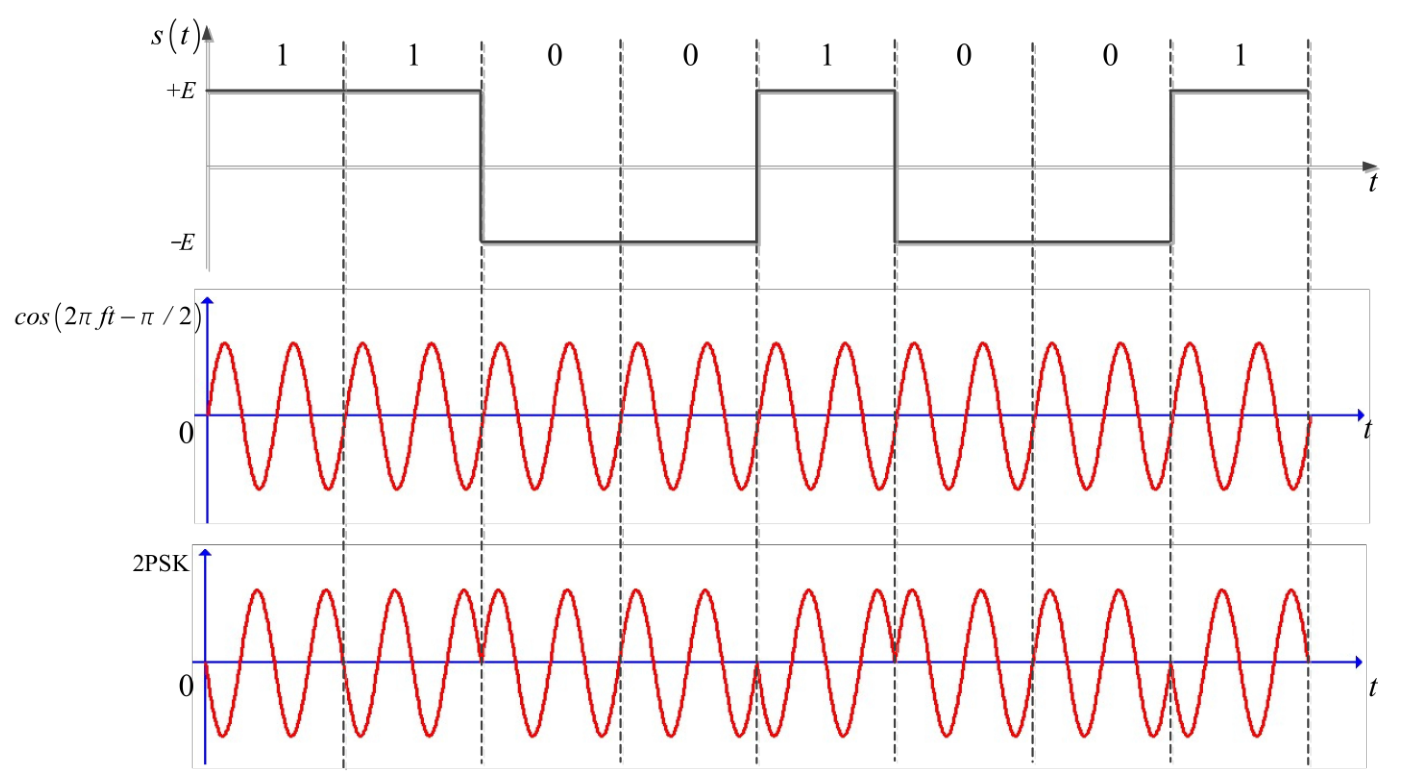
\includegraphics[width=0.83\textwidth]{ch02-psk-wave.png}
 \caption{2PSK以相差半周期的两种相位表达0与1。来源：\texttt{Chapter2-物理层.pdf}，PDF第65页（显示页65），波形局部截取。}
 \label{fig:psk-wave}
\end{figure}
\textbf{课件例题（PDF第65页／显示页65）：} 输入$11001001$，按“0取$\phi_0$、1取$\phi_0+\pi$”逐位查表，得到
\[
(\phi_0+\pi,\phi_0+\pi,\phi_0,\phi_0,\phi_0+\pi,\phi_0,\phi_0,\phi_0+\pi).
\]
代入课件的$\phi_0=-\pi/2$，绝对相位为
\[
(\pi/2,\pi/2,-\pi/2,-\pi/2,\pi/2,-\pi/2,-\pi/2,\pi/2).
\]
\annotationarea[4]

\textbf{2DPSK（二进制差分相移键控）}用相邻码元载波的相对相位变化表示信息。课件第66页约定：比特0使相位不变，记$\Delta\phi_n=0$；比特1使相位改变$\pi$，记$\Delta\phi_n=\pi$。因此第$n$个码元相位为前一码元相位加本位相位变化，可写成$y(t)=\cos(2\pi ft+\phi_{n-1}+\Delta\phi_n)$。接收端比较相邻码元相位即可解码，不必判断一个绝对相位基准。

\begin{figure}[H]
 \centering
 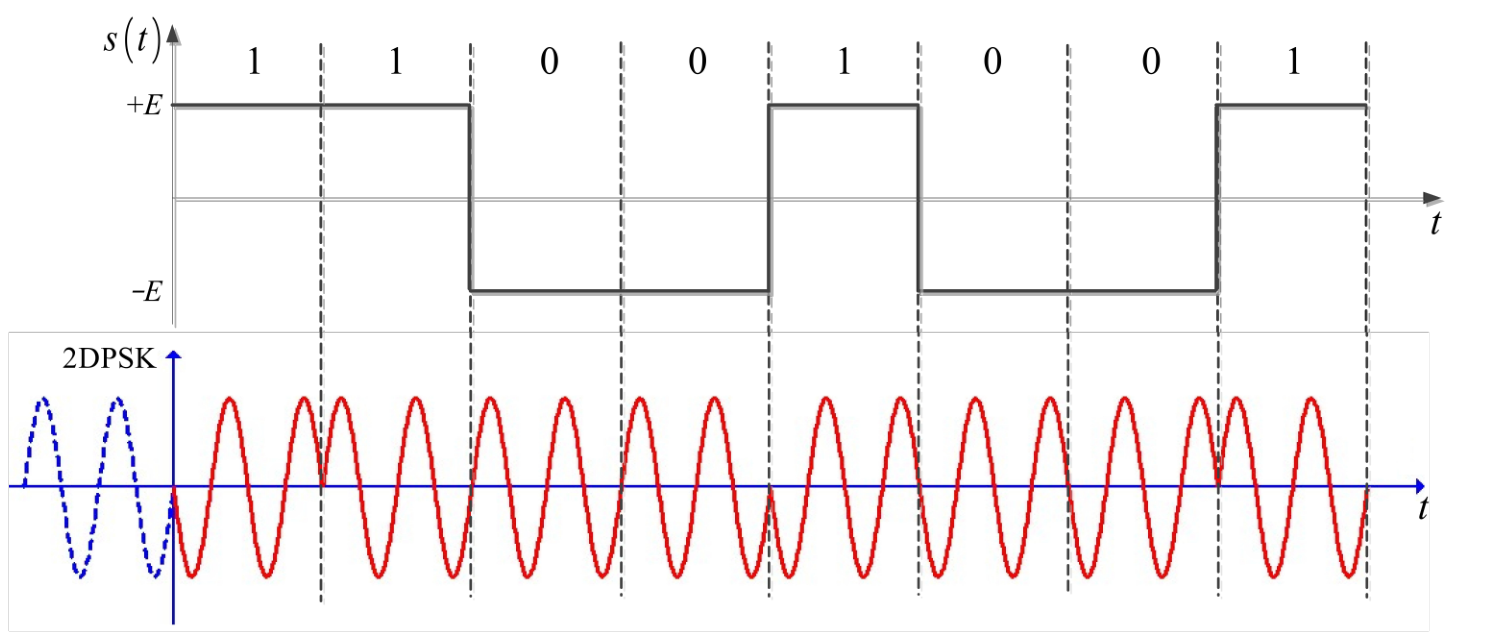
\includegraphics[width=0.92\textwidth]{ch02-dpsk-wave.png}
 \caption[2DPSK波形示意]{2DPSK例图中的虚线表示前一码元信号或初始参考载波。来源：Chapter2-物理层.pdf，PDF第67页（显示页67），局部截取。}
 \label{fig:dpsk-wave}
\end{figure}
图\ref{fig:dpsk-wave}中虚线是当前序列之前的参考，红色波形是已调信号；出现反相表示相位差$\pi$，相位连续表示相位差0。\textbf{课件例题（PDF第67页／显示页67）：} 输入$11001001$，以虚线参考相位$\phi_{-1}=0$为起点，依次累计相位变化$\pi,\pi,0,0,\pi,0,0,\pi$，各码元相位为$\pi,0,0,0,\pi,\pi,\pi,0$（模$2\pi$）。
\annotationarea[4]

\textbf{课件中的二进制调制性能比较（PDF第68页／显示页68）：}
\begin{center}
\small
\begin{tabularx}{0.97\textwidth}{l X}
\toprule
比较项目 & 课件给出的结论\\
\midrule
频带利用率 & 2ASK、2PSK、2DPSK相同；2FSK最低\\
误码率 & 在相同信噪比下，2PSK最低、2ASK最高；课件给出的抗噪声性能顺序为2PSK优于2FSK、2FSK优于2ASK\\
对信道特性变化的敏感性 & 2ASK较敏感；2FSK和2PSK较不敏感\\
\bottomrule
\end{tabularx}
\end{center}
这是课件采用的典型比较结论；具体系统比较还要核对信噪比定义、接收方式和其他条件。
\annotationarea[4]

\subsection{多进制与QAM：怎样阅读星座图}
二进制调制每码元只有两种状态，多进制调制让每码元选择更多状态。仍使用2.2节的关系
\[
 R_b=R_B\log_2M.
\]
\textbf{自拟例：} 1200 Baud、16种状态时，$R_b=1200\times4=4800$ b/s。若保持波特率不变而用64种状态，每码元6 bit，比特率变为7200 b/s；接收方要在同样时间里作更细致的状态区分。
\annotationarea[4]
课件同时指出，多进制数字调制需要更高的信噪比；发送端可增大发射信号功率以便接收端区分更多状态。
\annotationarea[4]

\textbf{正交幅度调制（QAM，Quadrature Amplitude Modulation）}又称幅值相位联合键控（APK），组合两条同频、相差$90^\circ$的载波。课件指出QAM频带利用率高、设备较简单，并可自适应调整调制速率。在课件记号下，一码元区间内的信号为
\[
 y(t)=A_n\cos(2\pi ft)+B_n\sin(2\pi ft),
\]
其中$A_n$、$B_n$分别控制同相I支路与正交Q支路的幅度，可取带正负号的离散值。课件也把合成信号写成$y(t)=s_n\cos(2\pi ft+\phi_n)$，其中$A_n=s_n\cos\phi_n$、$B_n=-s_n\sin\phi_n$；$s_n$和$\phi_n$分别表示该码元合成载波的幅度与相位。这里“正交”指两种基函数在一个合适码元区间上的内积为0，因此接收端可分别估计I、Q分量。

\textbf{星座图怎样看？} 横轴I和纵轴Q分别记两支路幅度，每个点$(A_n,B_n)$代表一种合成信号状态。到原点的距离与合成幅度对应，围绕原点的方向与合成相位对应（正负相位约定依系统）。方形16QAM每支路有4个可选幅度，组合为$4\times4=16$个点，每点对应4 bit；方形64QAM每支路有8个幅度，共64点，每点6 bit。接收方估计I/Q分量并判定最接近哪个合法点，然后恢复该点对应的比特组合。

\begin{figure}[H]
 \centering
 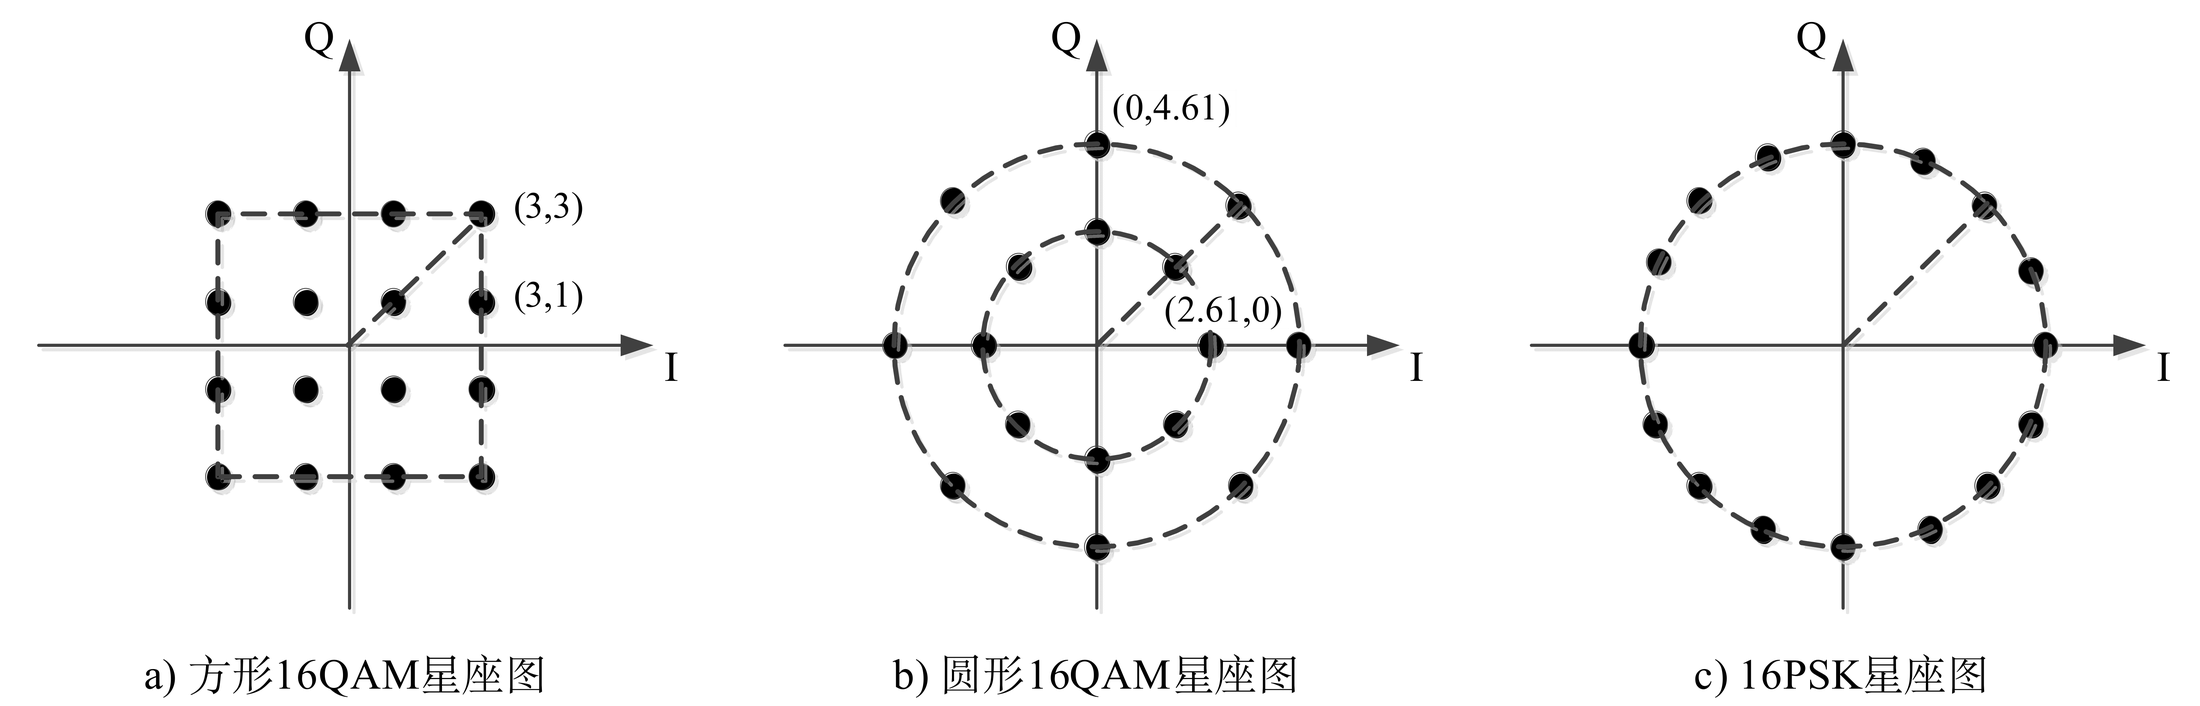
\includegraphics[width=0.93\textwidth]{ch02-qam.png}
 \caption{左：方形16QAM；中：圆形16QAM；右：16PSK对照图。来源：\texttt{Chapter2-物理层.pdf}，PDF第71页（显示页71），星座图局部截取。右图各点在同一圆周上，区别主要在相位，不应称为QAM图。}
 \label{fig:qam-constellation}
\end{figure}

课件第30页题目说“4相位、每相位4幅度”，直接按题设得到16状态；不要把它误当作方形16QAM必定只有4个极角。\textbf{学习补充：} 在同样平均发送功率下，星座点越多通常越拥挤，噪声更容易使接收点跨入邻点的判决区域，往往要求更高信噪比。QAM可提高频带利用率，但“QAM抗噪能力强”不能脱离阶数、能量和接收条件作绝对比较。

\textbf{易错点。} 编码是确定数字表示/线路码的规则；数字调制是控制载波状态。本章不同处理可连续使用，例如先把语音PCM数字化，再做冗余编码，再用QAM发送。Hz是频带宽度，Baud是码元数，bit/s是信息比特数；三种单位仍须分别保留。

\begin{quote}\small 来源：课件PDF第58--71页（显示页58--71）；教材§2.1.3，PDF第45--46页／印刷第34--35页。课件典型性能比较的条件在正文中显式提示，避免把示例结论推广为所有实现的排名。\end{quote}
\annotationarea[4]

\section{物理层设备}
\subsection{中继器：再生信号}
信号经过较长线路会减弱、变形。\textbf{中继器（Repeater）}按接收到的信号恢复应有的比特时序和波形，再向后发送，扩大可覆盖距离。图\ref{fig:repeater-regeneration}左侧是衰减失真的脉冲，右侧是再生后的规整脉冲。它的原理是再生，不能只理解为把电压乘一个系数；简单放大也会放大噪声。

\begin{figure}[H]
 \centering
 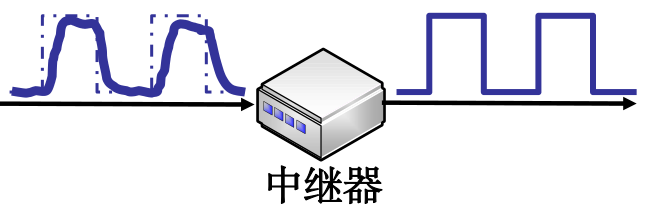
\includegraphics[width=0.68\textwidth]{ch02-repeater-regeneration.png}
 \caption{中继器将失真信号再生为规定波形。来源：\texttt{Chapter2-物理层.pdf}，PDF第73页（显示页73），局部截取。}
 \label{fig:repeater-regeneration}
\end{figure}

\textbf{适用边界。} 中继器不理解MAC地址或帧内容，也不完成不同数据链路协议的转换。如果输入信号已被误判，再生只会把误判后的比特继续发出，不能当成可靠纠错器。中继器数量也受相应网络标准和传播时延限制，不能无限串联扩展一个网络。
\annotationarea[4]

\subsection{集线器：多端口中继器}
\textbf{集线器（Hub）}相当于多端口中继器：一个端口收到的信号会再生并转发到其他端口，课件称各端口在内部物理连通。它不查找目的地址，不决定某个帧应只去哪个端口，也不学习地址表。使用Hub连接多台主机，线缆在物理上呈星形，通信逻辑仍共享同一通路。

\textbf{参考书补充：} Hub的各端口属于同一\emph{冲突域}，即多个发送端可能同时发送并发生冲突的范围。它按信号扩散方式转发，不按目的地址筛选端口，因此也不能分割广播域。课件第73页只强调Hub是多端口中继器、所有端口内部物理连通，并列出10BASE-T和100BASE-T以太网应用；冲突域等概念由参考书用于进一步解释。
\annotationarea[4]

\begin{quote}\small 来源：课件PDF第72--74页（显示页72--74）；教材§2.3--§2.4，PDF第57--60页／印刷第46--49页。\end{quote}

\subsection*{本章回顾}
物理层在物理介质上实现比特流传输。数据通信先将数据变成适合信道传送的信号；信道类型和容量限制可达到的传输速率。物理介质分导引型与非导引型；奈奎斯特公式讨论理想无噪声、带宽受限的容量，香农公式讨论有噪声信道的容量上限。信道共享可用FDM、TDM、WDM和CDM。基带传输直接发送基带信号，频带传输通过调制载波适配带通信道。中继器和集线器是课件列出的物理层设备，均以比特再生为基本工作原理。
\annotationarea[4]

% 第3章按课件顺序重写；本章课件 PDF 页码与幻灯片显示页码相同。
\chapter{数据链路层与局域网}

\noindent 本章课件共 153 页，依次讲解数据链路层服务、差错检测与纠正、可靠数据传输、多路访问控制、局域网技术、PPP 和链路虚拟化。以下按课件的章节顺序整理。课件 PDF 页码与页面右下角显示页码相同；引用教材时同时标出 PDF 阅读器页与印刷页。

\section{数据链路层服务}

\subsection{数据链路层负责一段链路上的传输}
\textbf{结点（node）}是网络中的主机、路由器或交换机。\textbf{链路（link）}是连接相邻结点的通信信道，可以是有线链路、无线链路或局域网。这里的“相邻”指两个结点直接通过同一条链路通信。

数据链路层位于网络层和物理层之间：向下使用物理层提供的比特传输服务，向上向网络层提供明确的服务接口。它负责将网络层交下来的\textbf{数据报}封装成\textbf{帧（frame）}，并通过一条链路送到直接相连的下一结点。帧是第 2 层的协议数据单元，载荷通常是网络层数据报。

若主机 A 经路由器 R 向主机 B 发送数据，A--R 链路上的帧到达 R 后，R 取出其中的数据报；R 再将数据报封装为适合 R--B 链路的帧。数据报可跨越多条链路，帧则服务于当前一段链路。不同链路可以使用不同的帧格式。

局域网（Local Area Network，LAN）数据链路层常分为两个子层：\textbf{逻辑链路控制（Logical Link Control，LLC）}面向上层服务，\textbf{介质访问控制（Medium Access Control，MAC）}处理帧如何使用共享介质。课件图中的发送过程是“网络层数据报 → 数据链路层封装成帧 → 物理层发送比特”；接收过程按相反方向处理。

\annotationarea{4}

\subsection{组帧、帧同步与透明传输}
\textbf{组帧（framing）}是把网络层数据报封装为帧。\textbf{帧同步}是从物理层交付的连续比特流中识别每一帧的开始和结束。\textbf{透明传输}要求接收方还原出原始载荷，即使载荷本身含有与帧边界相同的字节或比特组合，也不能把数据误认成边界。

\paragraph{字节计数法。} 在帧首部放入帧长度或计数字段，接收方据此读出一帧。课件第 7 页的四帧示例分别标出 5、5、8、6 字节。若计数字段本身传错，例如把 5 读成 7，接收方就可能多读后续帧的两个字节，之后的边界也随之错位。因此，单独依赖计数字段容易因该字段出错而失去同步。

\paragraph{定界符与字节填充。} 用特殊字节 \texttt{FLAG}（例如 \texttt{0x7E}）表示边界。若载荷中也出现 \texttt{FLAG}，发送方在该字节前插入转义字节 \texttt{ESC}；载荷中的 \texttt{ESC} 自身也需转义。接收方在帧内部看到 \texttt{ESC} 时，将其后的字节还原为普通数据。
\begin{quote}\small
课件示意：原载荷 \texttt{A FLAG ESC B}；填充后为 \texttt{A ESC FLAG ESC ESC B}；线上帧在其前后再加边界 \texttt{FLAG}。接收方去掉两端边界，并按转义规则解码，恢复原载荷。
\end{quote}

\paragraph{定界符与比特填充。} 用比特串 \texttt{01111110} 表示帧边界。发送方只扫描帧内部的载荷，每出现连续 5 个 1 就插入一个 0；首尾的定界符不填充。接收方识别帧边界后，在帧内部每串连续 5 个 1 后删除发送方插入的 0。
\[
  \text{载荷 }01111110\quad\longrightarrow\quad
  \text{填充后 }011111010.
\]
原载荷的中间有连续 6 个 1；插入 0 后不再出现与定界符相同的连续 6 个 1。接收端删除填入的 0 后恢复原比特串。

\begin{figure}[H]
 \centering
 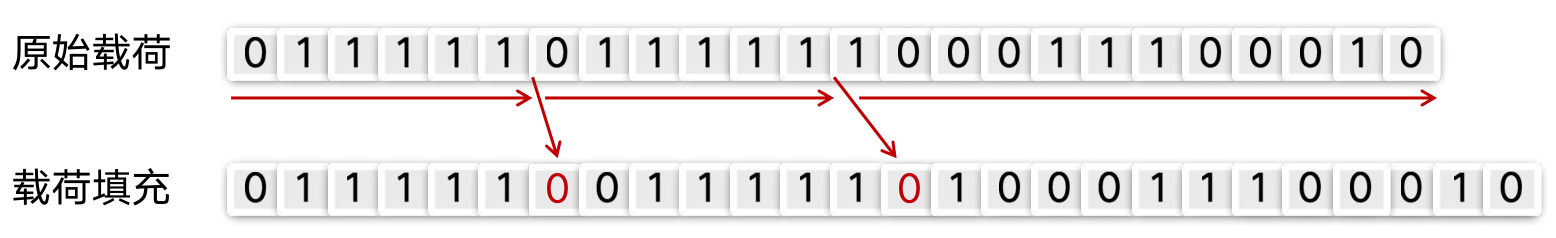
\includegraphics[width=0.82\textwidth]{ch03-bit-stuffing.png}
 \caption{帧内连续 5 个 1 后插入 0，接收时删除该 0。来源：\texttt{Chapter3-数据链路层.pdf}，PDF 第 11 页（显示页 11），局部截取。}
 \label{fig:ch03-bit-stuffing}
\end{figure}

\paragraph{物理层编码违例。} 若一种物理层编码有未使用的码字或信号模式，可把它用作边界。课件列举 4B/5B 编码中未使用的码字、传统以太网和 802.11 中的长前导码，以及曼彻斯特或差分曼彻斯特编码中比特周期中间无跳变的模式（课件以 802.5 令牌环为例）。该办法成立的前提是所选模式不会作为普通数据编码出现。

\annotationarea{4}

\subsection{链路层可能提供的其他服务}
数据链路层的功能不只组帧。不同协议会按需要提供下列服务，并非每种链路层协议都实现全部功能。

\begin{itemize}
 \item \textbf{物理寻址：}帧首部可以带有源和目的 MAC 地址，用于标识局域网内帧从哪个接口发出、交给哪个接口。MAC 地址的具体形式见“局域网技术”。
 \item \textbf{差错控制：}发送端可加入差错编码位，接收端检测帧是否损坏；某些编码可直接纠正错误，某些协议发现错误后请求重传，也有协议直接丢弃差错帧。
 \item \textbf{相邻结点间可靠交付：}通过确认、序号与重传等机制，处理损坏、丢失、乱序或重复。课件指出，无线链路误码率较高，常需要停等或滑动窗口机制；低误码率有线链路较少逐帧实现可靠传输。
 \item \textbf{流量控制：}协调相邻发送方与接收方的发送速度，避免接收端处理不过来或缓存耗尽。反馈式流量控制由接收方反馈状态，发送方据此调速；速率式流量控制由发送方按内建机制限速。
 \item \textbf{介质访问控制：}多个结点共用一个物理信道时，协调结点何时发送。
 \item \textbf{双工方式：}全双工允许链路两端同时双向传输；半双工允许双向通信，但两端交替发送。
 \item \textbf{服务类型：}无连接服务不先建立数据链路层连接；面向连接服务在交换数据前先建立连接。是否提供可靠交付是另一项独立属性。
\end{itemize}

\textbf{网卡（Network Interface Card，NIC）}或网络适配器实现数据链路层和物理层功能。它安装在主机或路由器的接口处，通过系统总线与主机相连，通常由控制器、硬件、固件和软件共同完成帧封装、比特发送、差错检测以及协议规定的流量控制和可靠传输。

\begin{quote}\small 来源：课件 PDF 第 3--16 页（显示页 3--16）；参考书 §3.1--§3.2，PDF 第 61--66 页（印刷第 50--55 页）。课件给出组帧、寻址、流量控制、差错控制、访问控制、半/全双工、连接服务和网卡实现等内容。\end{quote}
\annotationarea{4}

\section{差错检测与纠正}

\subsection{差错编码与汉明距离}
传输中的衰减和噪声可能导致比特翻转。发送方把原数据 $D$ 与若干\textbf{冗余比特} $R$ 组合成码字；接收方根据编码规则检查收到的码字。冗余位能提高检错或纠错能力，但任何有限编码都不能保证检测所有可能差错。

两个等长码字逐位比较时，不同位的个数称为\textbf{汉明距离}。例如，\texttt{0110} 与 \texttt{0011} 有两位不同，距离为 2。一个编码集合的最小汉明距离 $d_{\min}$，是所有不同合法码字之间距离的最小值。

课件给出的保证条件是：若 $d_{\min}=r+1$，可以检测任意不超过 $r$ 位的差错；若 $d_{\min}=2r+1$，可以纠正任意不超过 $r$ 位的差错。一般写成
\[
  \text{保证检出 }s\text{ 位错： }d_{\min}\ge s+1,\qquad
  \text{保证纠正 }t\text{ 位错： }d_{\min}\ge 2t+1.
\]
检错要求错误后的码字不落到另一个合法码字上；纠错还要求错误后的接收串离原码字比离其他合法码字更近。

\textbf{课件例题 1：检错码。} 编码集合为 $\{0000,0101,1010,1111\}$。任意两个不同码字至少有 2 位不同，因此 $d_{\min}=2$，能保证检测 1 位差错，但不能保证纠正 1 位差错。

\textbf{课件例题 2：纠错码。} 编码集合为 $\{000000,010101,101010,111111\}$，最小距离为 3，能保证纠正 1 位差错。若收到 \texttt{100010}，它与合法码字 \texttt{101010} 只差 1 位，因此在“最多 1 位差错”的前提下纠正为 \texttt{101010}。

\annotationarea{4}

\subsection{奇偶校验}
\textbf{一维奇偶校验}在数据后增加一个校验位，使码字中 1 的总数为偶数（偶校验）或奇数（奇校验）。若采用偶校验，任意奇数个比特翻转会改变 1 的个数奇偶性，因而可检测；偶数个比特翻转可能保持奇偶性，不能保证检测。一个校验位不能指出出错位置。

\textbf{二维奇偶校验}将数据位排成行和列，分别计算行、列校验位。若只有一个数据位翻转，会有且只有一行、 一列校验失败；行列交点就是错误位，可以据此纠正。多个错误可能使部分或全部行列校验再次满足，故不应把单比特定位的结论扩大到任意多比特错误。课件第 20 页将可纠错情形作了简写，使用时须带上“只有一个错误位”的条件。

\annotationarea{4}

\subsection{Internet 校验和}
Internet 校验和用于 IP、TCP、UDP 等协议的差错检测。发送方把待检内容按 16 位分组；最后不足 16 位的部分按规则补零。对各 16 位字进行反码加法：最高位产生的进位 1 回卷并加到最低位，若仍有进位则继续回卷。将最终和逐位取反，得到校验和并填入校验和字段。

接收端对收到的数据和校验和执行相同的 16 位反码加法。若数据与校验和相加为 16 个 1（再取反为全 0），检查通过；否则检出差错。检查通过只表示没有检出差错，并不保证传输绝对无错。

\annotationarea{4}

\subsection{循环冗余校验 CRC}
\textbf{循环冗余校验（Cyclic Redundancy Check，CRC）}使用模 2 除法生成检错位。模 2 加减法就是逐位异或 $\oplus$，不产生进位或借位，例如 $1\oplus1=0$、$1\oplus0=1$。

发送端与接收端预先约定生成比特串 $G$。若 $G$ 长度为 $r+1$ 位，则其对应多项式次数为 $r$。发送端在数据串 $D$ 后附加 $r$ 个 0，得到 $D\cdot 2^r$；用 $G$ 对其作模 2 长除，所得余数 $R$ 长度不超过 $r$ 位，必要时在左侧补 0 至 $r$ 位。发送的码字为 $D$ 后接 $R$。接收端用同一个 $G$ 除收到的完整码字：余数全 0 表示未检出差错，非零表示检出差错。

\textbf{课件例题（PDF p.23）。} 数据 $D=101110$，生成串 $G=1001$，因此 $r=3$，先补 3 个 0：
\[
 D\cdot 2^r=101110000.
\]
模 2 长除按每一步对齐最高位的 1 后异或：
\begin{center}
\begin{tabular}{c c}
\toprule
当前被除串 & 本步异或后的串\\
\midrule
\texttt{101110000} $\oplus$ \texttt{100100000} & \texttt{001010000}\\
\texttt{001010000} $\oplus$ \texttt{001001000} & \texttt{000011000}\\
\texttt{000011000} $\oplus$ \texttt{000010010} & \texttt{000001010}\\
\texttt{000001010} $\oplus$ \texttt{000001001} & \texttt{000000011}\\
\bottomrule
\end{tabular}
\end{center}
最后的余数为 3 位 $R=011$，所以发送 \texttt{101110011}。将其再除以 \texttt{1001}，余数为 \texttt{000}。

CRC 常用于帧的差错检测。课件指出，次数为 $r$ 的生成多项式能检测所有长度小于 $r+1$（即不超过 $r$）位的突发差错。\textbf{突发差错长度}从第一个错误位到最后一个错误位计数，中间即使有正确位也计入长度。更长突发错误通常也能检测，但不能保证全部检出。

\annotationarea{4}

\subsection{检错之后的处理}
差错处理有不同方案：\textbf{前向纠错（Forward Error Correction，FEC）}使用纠错码，让接收端在编码保证范围内直接修正比特；\textbf{检错重传}发现损坏后通过停等或滑动窗口协议请求再次发送；\textbf{检错丢弃}发现错误就丢弃帧；\textbf{反馈校验}将校验信息反馈给发送端。CRC 主要用于检错，不能单独恢复丢失帧。

\begin{quote}\small 来源：课件 PDF 第 17--24 页（显示页 17--24）；参考书 §3.3，PDF 第 67--71 页（印刷第 56--60 页）。CRC 例题采用课件第 23 页的 $D=101110$、$G=1001$；课件第 20 页二维奇偶校验的纠错能力按单比特差错条件表述。\end{quote}
\annotationarea{4}

\section{可靠数据传输}

\subsection{可靠传输的目标和协议接口}
可靠传输要求数据\textbf{不错、不丢、不乱、不多}：内容正确，没有缺失，按顺序交付，不重复交付。网络层、传输层和链路层都可能需要可靠传输机制。课件先用单向数据传输作为讲解模型，但确认等控制信息会沿反方向传送。

课件使用以下接口描述协议动作：\texttt{rdt\_send()} 表示上层交数据给可靠传输协议；\texttt{udt\_send()} 表示可靠传输协议把分组交给不可靠信道；\texttt{rdt\_rcv()} 表示分组到达接收方；\texttt{deliver\_data()} 表示接收方将数据交给上层。有限状态机（Finite State Machine，FSM）用状态记录协议正在等待什么；外部事件触发状态转移，并执行相应动作。

\annotationarea{4}

\subsection{rdt 1.0、2.0、2.1、2.2 与 3.0}
\textbf{rdt 1.0：可靠信道。} 假定底层信道不会出错也不会丢失分组。发送方收到上层数据后封装并发送；接收方收到后取出数据交给上层，不需要确认或重传。

\textbf{rdt 2.0：可能发生比特错误。} 发送方加入校验和；接收方正确收到后回送肯定确认（Acknowledgment，ACK），发现损坏后回送否定确认（Negative Acknowledgment，NAK）；发送方收到 NAK 后重传。基于反馈与重传的协议称为自动重传请求（Automatic Repeat reQuest，ARQ）。rdt 2.0 每次只发送一个分组并等待反馈，属于停等。其缺陷是 ACK/NAK 本身也可能损坏；发送方无法判断接收方是否已经收下数据，若直接重发便可能造成重复交付。

\textbf{rdt 2.1：使用序号识别重复分组。} 发送方交替使用序号 0 和 1。新分组使用下一个序号；同一分组重传时保留原序号。接收方记住期望序号：收到正确且期望的分组才交付一次并切换期望值；收到重复旧分组时不再次交付，但重新发送确认。此时假设分组不会完全丢失。

\textbf{课件思考：为什么 0 和 1 两个序号就够？} 停等时，发送方任一时刻最多有一个未确认的数据分组。接收方只需区分当前期望的新分组与上一个已接收分组的重传，因此 1 位序号（0、1 交替）即可。收到相同旧序号时，接收方知道是重复副本。

\textbf{rdt 2.2：不使用 NAK。} 接收方只发送 ACK，并在 ACK 中标明所确认分组的序号。若收到损坏或非期望分组，接收方再次确认最后一个正确收到的分组。发送方收到重复 ACK 时执行与 NAK 相同的动作，即重传当前分组。

\textbf{rdt 3.0：还可能发生分组丢失。} 发送方发送分组后启动计时器；收到正确且序号匹配的 ACK 后停止计时器。超过等待时间仍未收到 ACK，就重传原分组并重新计时。数据分组或 ACK 若只是延迟，重传可能产生重复分组，仍由序号机制识别。

\annotationarea{4}

\subsection{rdt 3.0 事件例题：无损、数据丢失与确认丢失}
课件 PDF 第 44--45 页用四条时间线说明停等协议。下表中的“交付”指接收方交给上层；“重复”指同一序号的旧副本。

\begin{enumerate}
 \item \textbf{无损：}发送方发送 pkt0；接收方收到并交付 pkt0，回 ACK0；发送方收到 ACK0 后发送 pkt1；接收方交付 pkt1 并回 ACK1。双方按序号交替继续。
 \item \textbf{数据分组丢失：}发送方发 pkt1，但该分组丢失；等待超时后仍用序号 1 重发 pkt1；接收方首次收到 pkt1 后交付并回 ACK1。
 \item \textbf{ACK 丢失：}接收方收到 pkt1 并交付，发出的 ACK1 丢失；发送方超时后重发 pkt1；接收方发现 pkt1 是重复副本，不再次交付，再回 ACK1；发送方收到后停止计时并可发送下一新分组。
 \item \textbf{过早超时：}发送方的计时器先于延迟的 ACK1 到期，于是重发 pkt1；接收方识别重复分组并再次回 ACK1。发送方收到一份匹配的 ACK1 后可继续；之后到达的重复 ACK 因序号不匹配当前状态而被忽略。
\end{enumerate}

\textbf{做题要点：}超时只说明发送方尚未得到确认，不能断定一定是数据分组丢失；可能丢的是 ACK，也可能只是延迟。接收方的序号检查负责去重，计时器负责打破无限等待。

\begin{figure}[H]
 \centering
 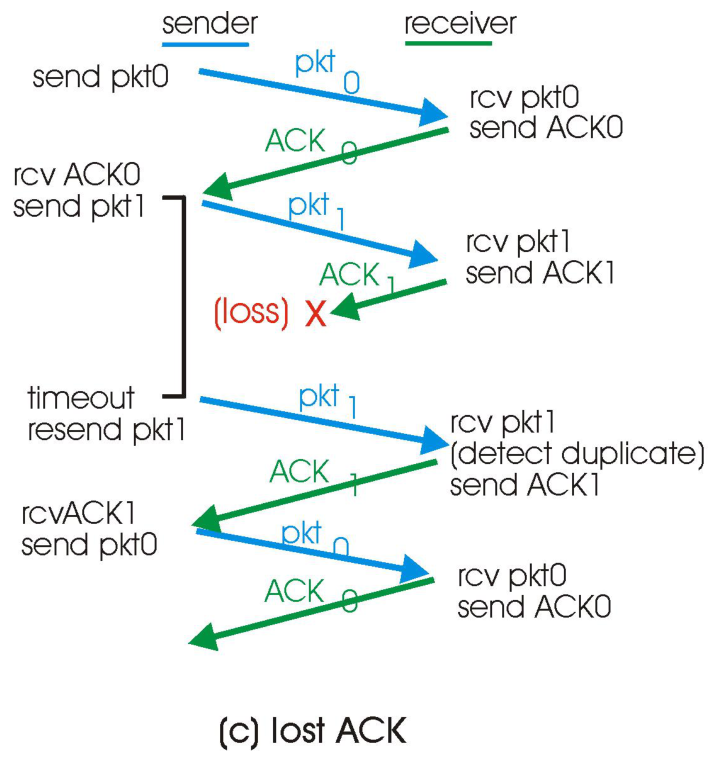
\includegraphics[width=0.9\textwidth]{ch03-ack-loss-detail.png}
 \caption{ACK 丢失后重传相同序号的分组，接收端识别重复并再次确认。时间向下，箭头表示分组或 ACK。来源：\texttt{Chapter3-数据链路层.pdf}，PDF 第 45 页（显示页 45），局部截取。}
 \label{fig:ch03-ack-loss}
\end{figure}

\annotationarea{4}

\subsection{停等协议的信道利用率}
设数据分组长 $L$ bit，发送速率 $R$ bit/s，则发送一个数据分组的时间为 $t_{\mathrm{seg}}=L/R$。确认分组长 $L_{\mathrm{ACK}}$ bit、反向链路速率 $R_{\mathrm{ACK}}$ bit/s，则确认发送时间 $t_{\mathrm{ACK}}=L_{\mathrm{ACK}}/R_{\mathrm{ACK}}$。\textbf{往返时间（Round-Trip Time，RTT）}按课件时间图理解：从数据分组最后一位发出，到 ACK 第一位返回发送端的往返等待时间；ACK 完整到达还需 $t_{\mathrm{ACK}}$。

从发送一帧开始到完整收到 ACK，一个停等周期为 $t_{\mathrm{seg}}+\mathrm{RTT}+t_{\mathrm{ACK}}$。无差错且收到确认后立即发送下一帧时，链路用于发送数据帧的比例为
\[
 U_{\mathrm{stop}}=
 \frac{t_{\mathrm{seg}}}{t_{\mathrm{seg}}+\mathrm{RTT}+t_{\mathrm{ACK}}}.
\]
它是发送端等待期间的时间利用率，不是载荷占帧长的比例。计算时须按题目给出的 RTT 定义，避免重复计算已经包含的时间。

\textbf{课件例题（PDF p.46--48）。} 链路速率为 $1\,\mathrm{Gb/s}$，单程传播延迟 $15\,\mathrm{ms}$，每个分组长 $1\,\mathrm{KB}=8000$ bit。忽略 ACK 发送时间，则
\[
 t_{\mathrm{seg}}=\frac{8000}{10^9}\,\mathrm{s}=8\,\mu\mathrm{s},\qquad
 \mathrm{RTT}=2\times15\,\mathrm{ms}=30\,\mathrm{ms},
\]
\[
 U\approx\frac{8\,\mu\mathrm{s}}{8\,\mu\mathrm{s}+30\,\mathrm{ms}}
 =0.0002666\approx0.0267\%.
\]
有效发送速率约为 $1\,\mathrm{Gb/s}\times U=267\,\mathrm{kb/s}$，即约 $33\,\mathrm{kB/s}$。物理线路很快，但停等发送方的大部分时间在等 ACK。

\annotationarea{4}

\subsection{流水线和滑动窗口}
\textbf{流水线}允许发送方在收到确认前连续发送多个分组，可以减少线路空闲时间，但要求序号空间更大，并在发送方、接收方或两端缓存尚未确认的分组。\textbf{窗口}是当前允许使用的一段序号范围；窗口尺寸为 $N$ 时，最多可有 $N$ 个分组等待确认。随着确认到达，窗口沿序号空间向前滑动。

\begin{figure}[H]
 \centering
 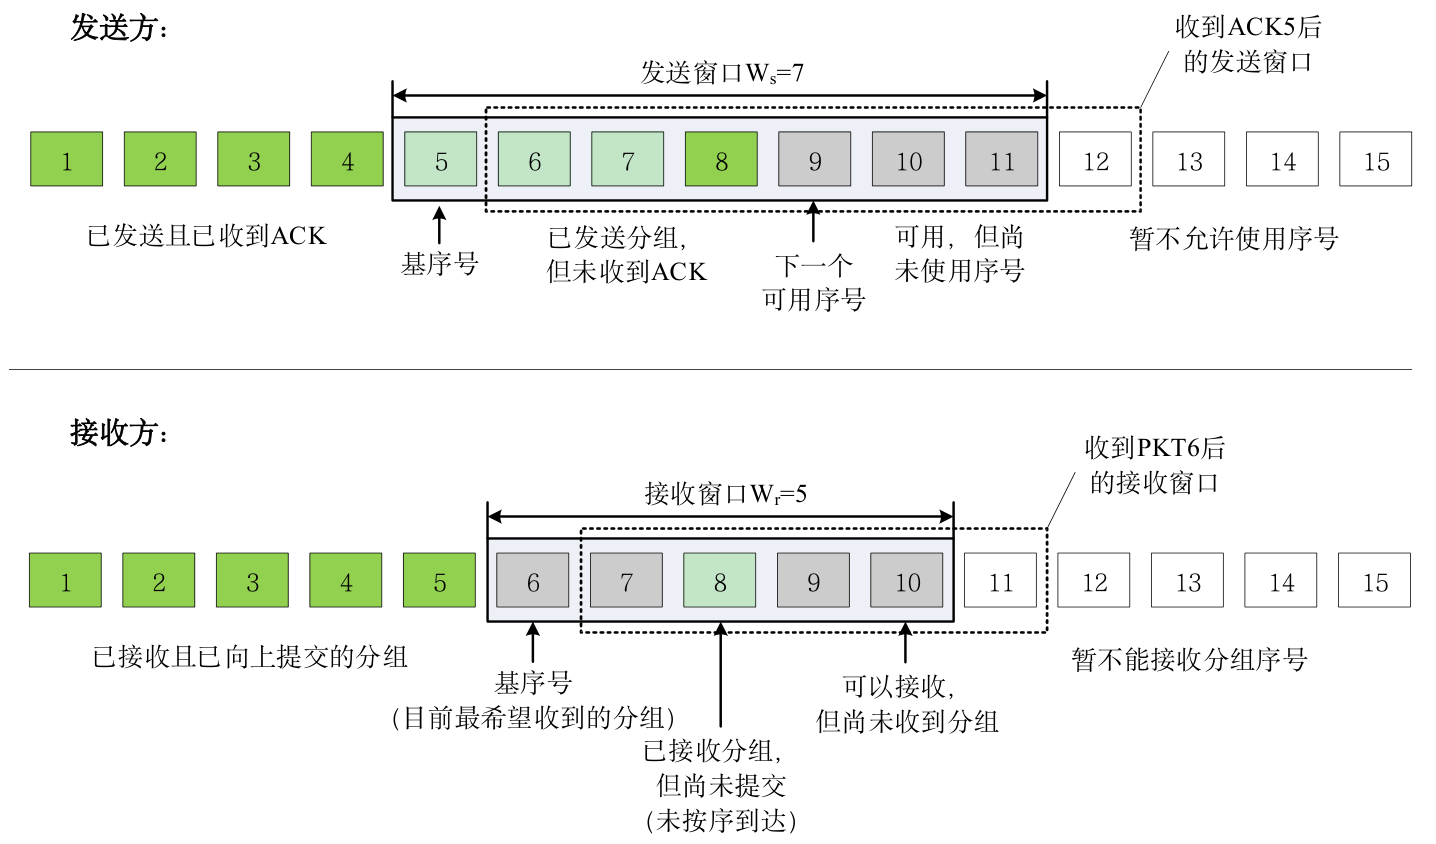
\includegraphics[width=0.88\textwidth]{ch03-sliding-window.png}
 \caption{发送窗口限制未确认分组；接收窗口限制可接收序号，窗口随确认或按序交付前移。来源：\texttt{Chapter3-数据链路层.pdf}，PDF 第 53 页（显示页 53），局部截取。}
 \label{fig:ch03-window}
\end{figure}

若序号字段有 $k$ bit，序号按模 $2^k$ 循环。课件给出的窗口约束为
\[
 W_s+W_r\le 2^k,
\]
其中 $W_s$ 是发送窗口尺寸，$W_r$ 是接收窗口尺寸。具体协议还需满足自己的限制：GBN 中 $W_r=1$，故 $W_s\le2^k-1$；典型 SR 取 $W_s=W_r=W$，因此 $W\le2^{k-1}$；停等取 $W_s=W_r=1$，至少需 $k=1$。

\textbf{课件思考：窗口大小影响什么？} 窗口增大后，允许同时有更多未确认分组，信道利用率和吞吐率可以提高；但发送和接收端要缓存更多分组，窗口还受序号空间、接收缓存、流量控制与拥塞控制条件限制。窗口并非越大越好，必须满足序号空间和接收能力的约束。

\annotationarea{4}

\subsection{后退 N 帧协议 GBN}
\textbf{后退 N 帧（Go-Back-N，GBN）}采用发送窗口 $W_s$ 和接收窗口 $W_r=1$。发送方可连续发送窗口内多个分组；接收方只接收当前期望的序号，乱序分组直接丢弃。

GBN 使用\textbf{累积确认}：ACK($n$) 表示按发送顺序截至序号 $n$（包含 $n$）的分组均已正确接收；序号回绕时按序号空间中的先后次序理解，而不是按普通整数大小比较。发送方可为最早未确认的分组设置计时器；该分组超时后，重传它以及之后所有已经发出但仍未确认的分组。接收方若收到乱序分组，会再次确认最近按序接收的分组。

\textbf{课件示例（PDF p.59）。} pkt2 在传输中丢失。接收方收到 pkt0、pkt1 后依次确认；pkt3、pkt4、pkt5 因不等于当前期望的 pkt2 而被丢弃，并重复确认 pkt1。发送方收到 ACK0、ACK1 后可继续发 pkt4、pkt5；pkt2 超时后，按 GBN 规则依次重发 pkt2、pkt3、pkt4、pkt5。接收方此后按序收到并交付这些分组。

\textbf{课件例题（PDF p.60）。} 发送方已经发送 0--7 号帧；计时器超时时只收到 0、2、3 号帧的确认。需要重发多少帧，分别是哪几帧？

\textbf{解：}GBN 确认是累积确认。最高连续确认到 3 号，因此 4、5、6、7 号帧尚未得到确认；超时后需要重发 4 帧，即 4、5、6、7 号帧。

\annotationarea{4}

\subsection{选择重传协议 SR}
\textbf{选择重传（Selective Repeat，SR）}对每个正确收到的分组分别确认。接收方把窗口内到达的乱序分组暂存，等缺少的较早分组到达后，再按序将连续分组交给上层。发送方只重传未确认的分组，并为每个未确认分组单独设置计时器。

\textbf{课件示例（PDF p.65）。} 发送窗口、接收窗口均为 4。发送 pkt0、pkt1 后，pkt2 丢失，pkt3 仍可发送。接收方收到 pkt0、pkt1，分别交付并回 ACK0、ACK1；pkt3 在接收窗口内但乱序到达，于是缓存并回 ACK3。发送方收到 ACK0 后发 pkt4，收到 ACK1 后发 pkt5；接收方将 pkt4、pkt5 缓存并分别确认。pkt2 超时，发送方只重发 pkt2。接收方收到 pkt2 后，连续交付缓存中的 pkt2、pkt3、pkt4、pkt5，接收窗口前移。

\textbf{窗口与序号的歧义例（课件 PDF p.66--67）。} 若序号只有 2 bit，则序号为 0、1、2、3。SR 的发送和接收窗口若都为 3，就有 $W_s+W_r=6>4$。接收窗口滑动后可能同时包含序号 0；此时收到 0，接收方无法只凭序号判断它是上一轮迟到的旧副本，还是新一轮的 0 号分组。故典型等大窗口必须满足 $W\le2^{k-1}$；$k=2$ 时最大窗口为 2。

\textbf{课件思考：SR 还能怎样设计？} 可以改变确认和缓存的实现细节，但任何变体都必须规定每个分组如何确认、乱序数据如何暂存和按序交付，并保证新旧序号不会发生歧义。课件给出的 SR 是本章采用的典型设计。

\begin{figure}[H]
 \centering
 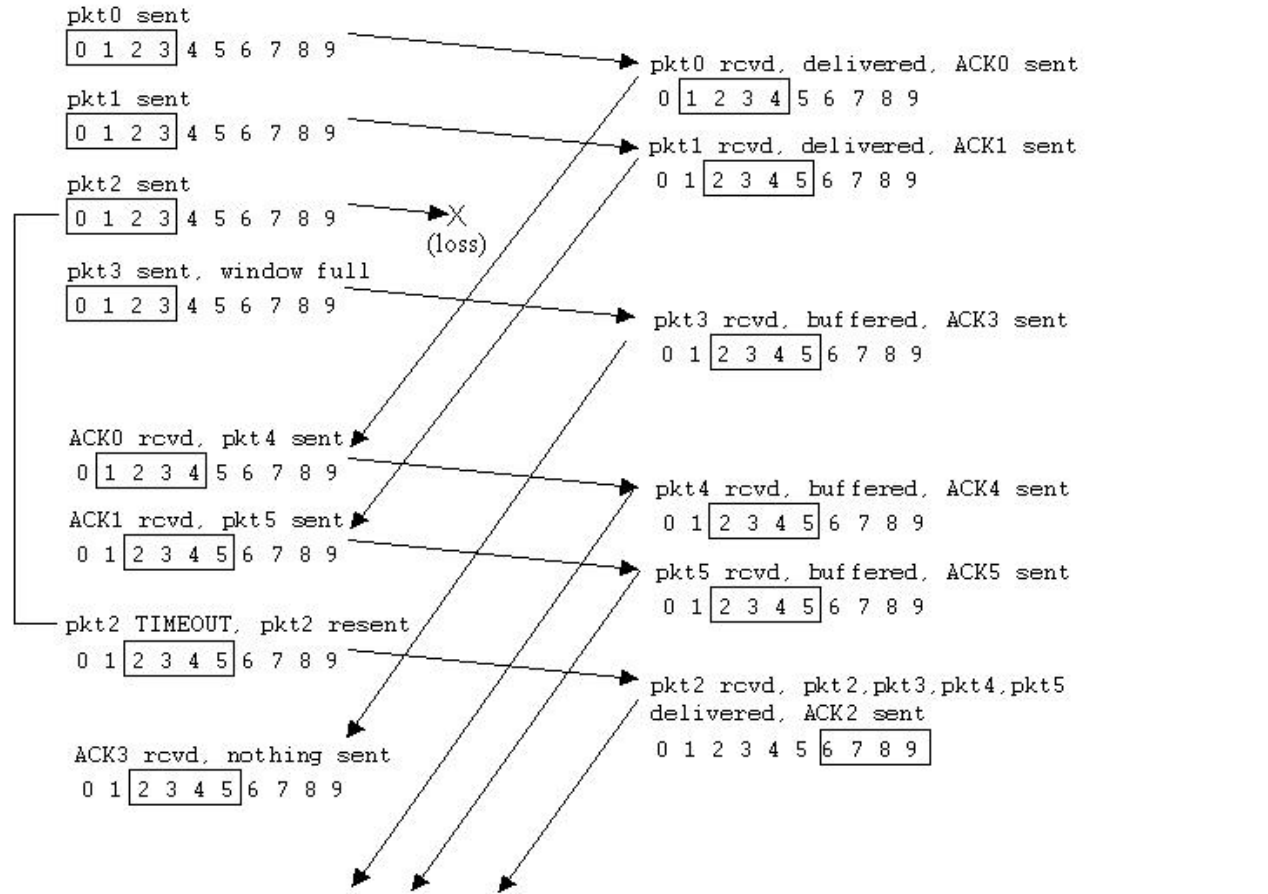
\includegraphics[width=0.98\textwidth]{ch03-sr-run-detail.png}
 \caption{SR 对 pkt0、pkt1、pkt3 等逐个确认并缓存乱序分组；pkt2 重传到达后按序交付缓存分组。来源：\texttt{Chapter3-数据链路层.pdf}，PDF 第 65 页（显示页 65），局部截取。}
 \label{fig:ch03-sr-run}
\end{figure}

\annotationarea{4}

\subsection{滑动窗口的利用率}
设连续发送窗口可容纳 $W_s$ 个分组，每个分组发送时间为 $t_{\mathrm{seg}}$，RTT 和 ACK 发送时间与停等定义相同。在无差错且发送端始终有数据时，窗口提供的理论利用率为
\[
 U=\min\!\left(1,\frac{W_s\,t_{\mathrm{seg}}}
 {t_{\mathrm{seg}}+\mathrm{RTT}+t_{\mathrm{ACK}}}\right).
\]
若 $W_s t_{\mathrm{seg}}$ 不足以覆盖一个确认往返周期，窗口耗尽后发送方仍需等待；当窗口能覆盖整个周期时，发送端可持续发送，利用率达到 1。实际吞吐还会受差错、重传、接收能力和可用带宽影响。

\begin{quote}\small 来源：课件 PDF 第 25--68 页（显示页 25--68）；参考书 §3.4，PDF 第 72--87 页（印刷第 61--76 页）。课件例题与事件图：rdt 3.0 第 44--45 页，停等性能第 46--48 页，GBN 第 59--60 页，SR 第 65--67 页。窗口上限按课件第 67 页所列约束表述。\end{quote}
\annotationarea{4}

\section{多路访问控制协议}

\subsection{共享广播信道和理想 MAC}
\textbf{点对点链路}只有两个通信端，例如拨号 PPP 或主机与交换机之间的专用链路。\textbf{广播链路}由多个结点共享，例如早期总线以太网、802.11 无线局域网。两个或更多结点同时在同一共享信道上传输，信号会相互干扰并发生\textbf{冲突（collision）}，接收失败。

\textbf{多路访问控制（MAC）协议}以分布式规则决定共享信道上的结点何时传输；协调信息也通过共享信道传送，没有另设带外协调信道。理想 MAC 希望：只有一个结点发送时可用全部速率 $R$；有 $M$ 个结点发送时平均每个结点获得 $R/M$；不依赖特定中心结点和同步时钟，并且规则简单。

课件将 MAC 协议分为三类：\textbf{信道划分}（预先分配时间、频率或编码资源）、\textbf{随机访问}（允许竞争与冲突，再通过规则恢复）、\textbf{轮转访问}（按顺序把发送机会交给结点）。

三类机制在不同负载下的取舍不同：信道划分在负载重时可稳定、公平地分享信道，但负载轻时未使用的预留资源会空闲；随机访问在负载轻时，单个结点可使用整个信道速率，负载重时冲突开销增加；轮转访问试图综合两者的优点。

\annotationarea{4}

\subsection{信道划分：TDMA、FDMA、CDMA 和 WDMA}
\textbf{时分多路访问（Time Division Multiple Access，TDMA）}把时间按周期分成固定时隙，每个站每周期使用指定时隙。若站点没有数据，其时隙仍空闲。课件例子中 6 个站点各有一个时隙，只有站点 1、3、4 发送，站点 2、5、6 的时隙未用。

\textbf{频分多路访问（Frequency Division Multiple Access，FDMA）}把信道频谱分成若干频带，每个站使用固定频带。无数据的站所分频带空闲。与 TDMA 不同，多个频带可在同一时刻同时传输。

课件还列出\textbf{码分多路访问（Code Division Multiple Access，CDMA）}和\textbf{波分多路访问（Wavelength Division Multiple Access，WDMA）}。CDMA 用不同码片序列区分同一信道上的信号；参考书补充说明，发送端用自己的码片表示 1、用反码表示 0，多站信号线性叠加，码片序列互相正交时，接收端与目标码片序列作规格化内积即可分离目标信号。WDMA 是光纤中的波长划分，各波长承载不同信号。

\textbf{课件比较要点：}TDMA 按时间切分，FDMA 按频带切分，CDMA 按码区分；预分配资源使忙时较稳定，但轻载时未使用的时隙、频带或码资源不能总被其他站点利用。

\annotationarea{4}

\subsection{随机访问：时隙 ALOHA 与纯 ALOHA}
随机访问允许结点在需要时使用信道的全部数据速率 $R$，无需事先预约；多个结点同时发送时会冲突，协议必须定义如何检测或判断冲突，以及如何延迟重传。

\textbf{时隙 ALOHA}把时间划为等长时隙，一帧恰可在一个时隙内发送，且所有结点同步。结点只能在时隙开始时发送。有新帧时在下一时隙发送；若冲突，后续时隙以概率 $p$ 重传，直到成功。单个结点发送时可连续使用全信道速率；空闲时隙和冲突时隙会浪费资源。

设有 $N$ 个结点且每个结点一直有数据，任一结点每时隙独立地以概率 $p$ 发送。指定结点成功的概率为 $p(1-p)^{N-1}$，任意结点成功的概率（即该时隙成功传输的期望比例）为
\[
 S_{\mathrm{slot}}=Np(1-p)^{N-1}.
\]
取 $p=1/N$ 可使其最大；当 $N$ 很大时，最大效率趋近 $1/e\approx0.37$，其中 $e\approx2.71828$ 是自然对数的底。效率是长期观察中成功传输的时隙比例。

\textbf{纯 ALOHA}不把时间划为时隙，新帧到达后立即发送，不要求时钟同步。若帧发送时间为一个单位时长，某帧会与其开始发送前后各一个帧时长内开始的其他帧相冲突，易受冲突影响的时间范围是时隙 ALOHA 的两倍。指定结点成功概率为
\[
 p(1-p)^{2(N-1)},
\]
任一结点成功的概率为 $Np(1-p)^{2(N-1)}$。结点数很多时，最大效率趋近 $1/(2e)\approx0.18$，低于时隙 ALOHA。

\annotationarea{4}

\subsection{载波监听 CSMA}
\textbf{载波监听多路访问（Carrier Sense Multiple Access，CSMA）}要求结点在发送前先监听信道：空闲就发送完整帧，忙则推迟。由于信号传播需要时间，远处结点可能还没有听到另一结点的信号而误以为空闲，所以 CSMA 仍可能发生冲突。冲突帧继续传输会浪费信道资源。

课件列出三种坚持规则：\textbf{1-坚持 CSMA}在信道空闲时立即发送，忙时持续监听；\textbf{非坚持 CSMA}遇忙后等待随机时间，再重新监听；\textbf{$p$-坚持 CSMA}适用于时隙信道，空闲时以概率 $p$ 发送，以概率 $1-p$ 延至下一时隙。

\textbf{载波监听与冲突检测（Collision Detection，CD）结合为 CSMA/CD。} 它适用于有线局域网，发送站在发送时继续监听信道，检测到冲突就立即中止发送，并可发出拥塞信号以通知其他站点。课件概括为“边发边听，不发不听”。有线结点可比较信道上的电压或接收信号与自身发送信号；无线结点的接收信号容易被本地发射信号淹没，难以用同样方法检测冲突。

课件第 95 页还把\textbf{载波监听多路访问/冲突避免（Carrier Sense Multiple Access with Collision Avoidance，CSMA/CA）}列为 802.11 无线局域网所用的随机访问协议。本章课件仅在总结页列出该名称，未展开其步骤。

\annotationarea{4}

\subsection{CSMA/CD 的争用期与最小帧长}
设冲突域中最远两站距离为 $d_{\max}$，信号传播速度为 $V$ m/s，链路速率为 $R$ bit/s。最远两站间的往返传播时间为 $2d_{\max}/V$。为保证发送端在完成发送前仍有机会检测到最远端发生的冲突，必须满足
\[
 \frac{L_{\min}}{R}\ge \frac{2d_{\max}}{V},\qquad
 L_{\min}\ge \frac{2d_{\max}R}{V},
\]
其中 $L_{\min}$ 是以 bit 计的最小帧长。等号对应临界设计。提高速率或增大网络距离会要求更大的最小帧，缩短距离或降低速率则可减小最小帧。

\textbf{课件例题（PDF p.86）。} CSMA/CD 网络速率 $R=1\,\mathrm{Gb/s}=10^9$ bit/s，电缆信号速度 $V=200000\,\mathrm{km/s}=2\times10^8$ m/s。若最小帧长减少 800 bit，最远两站距离至少怎样变化？

\textbf{解：}由 $d_{\max}=VL_{\min}/(2R)$，有
\[
 \Delta d_{\max}=\frac{V}{2R}\Delta L_{\min}
 =\frac{2\times10^8}{2\times10^9}(-800)\,\mathrm{m}
 =-80\,\mathrm{m}.
\]
距离需减少 80 m，选 D。

\annotationarea{4}

\textbf{课件给出的 CSMA/CD 效率近似式}为
\[
 \eta\approx\frac{1}{1+5t_{\mathrm{prop}}/t_{\mathrm{trans}}},
\]
其中 $t_{\mathrm{prop}}$ 是 LAN 中两结点间最大传播延迟，$t_{\mathrm{trans}}$ 是最长帧的传输时间。传播延迟相对帧传输时间越小，效率越接近 1；传播时延趋近 0 或帧传输时间趋于很大时，课件给出的效率极限为 1。

\annotationarea{4}

\subsection{轮转访问与比特映像}
\textbf{轮询（polling）}由主结点按次序邀请从属结点发送，适合简单从属设备。优点是不会因多个受控站同时发送而冲突；缺点是轮询本身有开销、站点要等待轮到自己，主结点还可能成为单点故障。

\textbf{令牌传递（token passing）}让特殊控制帧“令牌”按次序从一个结点传给下一个；持有令牌的结点获得发送机会。它无需中央主结点逐站轮询，但令牌传递有开销和等待延迟，令牌控制也可能成为故障点。

\textbf{比特映像介质访问控制}把周期分为预约期和数据发送期。若有 $N$ 个站，预约期含 $N$ 个 1 bit 时隙，每个站在自己的时隙发送 1 表示有帧待发；预约结束后，已预约站按编号顺序发送，因而不会发生发送冲突。每周期固定的预约开销是 $N$ bit。

课件总结将蓝牙、光纤分布式数据接口（Fiber Distributed Data Interface，FDDI）和令牌环列作轮转访问机制的相关应用或技术例子。

\textbf{课件思考：轮询和令牌传递有何异同？}二者都轮流分配发送机会，可避免竞争冲突，都有控制开销、等待延迟和控制机制故障风险。轮询由主结点集中分配机会；令牌传递由令牌按次序在结点间传递机会。课件还列比特映像作为另一种预约后顺序发送的方法。

\textbf{课件思考：能否设计新的轮转访问方案？}可以提出满足规则的方案，但课件没有给唯一答案。方案须说明谁有权发送、怎样传给下一站、如何保证同一时刻不发生冲突，并交代预约开销、等待时间和控制信息失效时如何恢复。答题时可用课件已有的轮询、令牌或比特映像机制说明设计思路，不需要为方案另造协议名称。

\annotationarea{4}

\begin{quote}\small 来源：课件 PDF 第 69--95 页（显示页 69--95）；参考书 §3.5，PDF 第 88--97 页（印刷第 77--86 页）。课件例题：CSMA/CD 最小帧长与距离，第 86 页。CDMA 码片说明、WDM 对应波长复用见参考书 §3.5.1，PDF 第 90--91 页（印刷第 79--80 页），作为课件所列术语的简要补充。\end{quote}

\section{局域网技术}

\subsection{MAC 地址与 IP 地址}
数据链路层需要在当前局域网中标识发送和接收接口。大多数局域网（Local Area Network，LAN）使用 48 bit 的\textbf{介质访问控制（Medium Access Control，MAC）地址}，也称 LAN 地址、物理地址或以太网地址，通常以 6 组十六进制数表示，例如 \texttt{1A-2F-BB-76-09-AD}。电气电子工程师学会（Institute of Electrical and Electronics Engineers，IEEE）管理并分配 MAC 地址空间；课件指出，前 24 bit 是厂商代码，后 24 bit 由厂商用于区分其网卡。MAC 地址可由网卡提供，也可由软件设置；以太网广播地址为 \texttt{FF-FF-FF-FF-FF-FF}。网卡收到帧后检查目的地址：目的为本机、广播地址或本机应接收的组播地址时接收，否则丢弃。

\textbf{网际协议（Internet Protocol，IP）地址}是网络层地址，例如第 4 版网际协议（IPv4）地址为 32 bit，标识网络层接口并用于跨网络转发。MAC 地址用于当前链路上的帧交付；IP 地址用于网络层分组转发。MAC 地址是平面地址，通常不编码网络层次；IP 地址按网络组织而具有层次性。课件用“MAC 地址像身份证号、IP 地址像邮政地址”说明两者用途不同。

\annotationarea{4}

\subsection{以太网拓扑、服务与 CSMA/CD 算法}
\textbf{以太网（Ethernet）}是广泛使用的有线局域网技术，课件强调它结构简单、成本较低，且已有多种速率可满足网络需求。早期总线拓扑中多个结点共用同一介质，处于一个冲突域；目前常见星形拓扑以交换机为中心，每个主机连接独立端口。

以太网 MAC 层提供\textbf{无连接、不可靠}服务：发送帧前不与接收网卡握手，接收网卡不逐帧向发送网卡确认；发现差错的帧会被丢弃，数据恢复由高层协议承担。CSMA/CD 的碰撞处理只说明发送结点是否检测到冲突，不等于接收端确认了数据交付。

课件第 103 页给出共享式以太网网卡的 CSMA/CD 流程：
\begin{enumerate}
 \item 网卡从网络层取得数据报并构造帧。
 \item 监听信道。空闲就开始发送；忙则持续等待到空闲后发送。
 \item 若发送完整帧时没有检测到冲突，网卡按本协议判断发送成功。
 \item 检测到冲突时停止发送并发出 jam signal（拥塞信号）。
 \item 执行截断二进制指数退避。连续第 $m$ 次冲突后令 $n=\min(m,10)$，从 $\{0,1,\ldots,2^n-1\}$ 中随机选择 $K$，等待 $K\times512$ 个比特时间后重新监听。一个比特时间是线路发送 1 bit 所需的时间 $1/R$。
\end{enumerate}
冲突次数越多，随机等待范围越大，降低冲突后立即再次相撞的可能。

\textbf{半双工与全双工。} 共享介质、集线器连接或半双工链路要依靠 CSMA/CD 协调。主机与交换机直接连接的独享全双工链路可同时双向传输，不发生共享介质碰撞，因此不运行 CSMA/CD。课件第 114 页把“每段链路使用 CSMA/CD”与“无冲突且可全双工”放在同一页，须按链路类型区分：半双工共享链路才需冲突检测，全双工专用链路不需 CSMA/CD。

\annotationarea{4}

\subsection{以太网帧格式与长度}
课件列出 DIX（DEC、Intel、Xerox）Ethernet V2 与 IEEE 802.3 两种格式。二者的字段顺序相近；源、目的地址各占 6 B，之后的 2 B 在 Ethernet II 中表示载荷协议类型，在 802.3 中表示长度。普通 MAC 帧还含数据和 4 B 帧检验序列（Frame Check Sequence，FCS）。

\begin{center}
\begin{tabularx}{0.98\textwidth}{l l X}
\toprule
字段 & 字节数 & 含义\\
\midrule
目的 MAC 地址 & 6 & 接收网卡检查的链路层目的地址\\
源 MAC 地址 & 6 & 发出该帧的网卡地址\\
Type / Length & 2 & Ethernet II 表示上层协议；802.3 表示长度\\
数据与填充 & 46--1500 & 上层协议载荷，不足 46 B 时填充\\
FCS & 4 & CRC 检错字段\\
\bottomrule
\end{tabularx}
\end{center}

发送端还会先发送 8 B 前导码：前 7 B 为 \texttt{10101010}，第 8 B 为 \texttt{10101011}，用于时钟同步和帧开始定位，通常不计入 MAC 帧长。MAC 帧固定字段合计 $6+6+2+4=18$ B；因此普通无标签帧的最小总长 $18+46=64$ B，最大总长 $18+1500=1518$ B。最大数据载荷 1500 B 也称最大传送单元（Maximum Transmission Unit，MTU）；它不是整个帧的长度。

\textbf{课件例：最小帧时间。} 10 Mb/s 以太网的争用期为 512 个比特时间，因此
\[
 t_{\mathrm{slot}}=\frac{512\,\mathrm{bit}}{10\times10^6\,\mathrm{bit/s}}
 =51.2\,\mu\mathrm{s},\qquad L_{\min}=512\,\mathrm{bit}=64\,\mathrm{B}.
\]
数据区至少 46 B，以便包含 18 B 固定开销后达到 64 B。课件 PDF 第 105 页把时间写成 $512\,\mu\mathrm{s}$，与 $512$ bit、$10$ Mb/s 的计算不一致；应为 $51.2\,\mu\mathrm{s}$。

\begin{figure}[H]
 \centering
 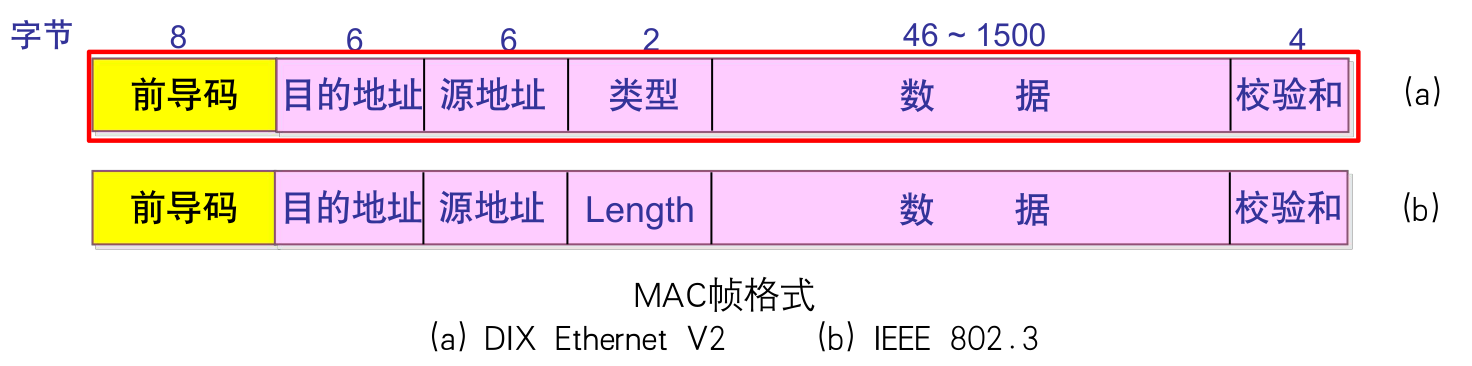
\includegraphics[width=0.95\textwidth]{ch03-ethernet-frame.png}
 \caption{Ethernet II 与 IEEE 802.3 帧的 2 B 字段分别表示 Type 和 Length；前导码通常不计入 MAC 帧长。来源：\texttt{Chapter3-数据链路层.pdf}，PDF 第 104 页（显示页 104），局部截取。}
 \label{fig:ch03-ethernet-frame}
\end{figure}

\annotationarea{4}

\subsection{以太网速率和物理层演进}
不同以太网标准通常保持 MAC 协议和基本帧格式，主要改变速率、物理介质和编码。课件列举 10 Mb/s、100 Mb/s、1 Gb/s、10 Gb/s、40/100 Gb/s 及更高速率，并比较光纤、铜缆和不同编码。

\begin{itemize}
 \item \textbf{快速以太网 100BASE-T：}速率为 100 Mb/s；BASE 表示基带传输，T 表示双绞线介质。
 \item \textbf{千兆以太网：}由 100 Mb/s 发展到 1 Gb/s，保留原有帧格式和基本工作方式。半双工模式为兼容可使用 CSMA/CD、载波扩充和帧突发；默认的全双工模式不使用 CSMA/CD。
 \item \textbf{万兆以太网：}10 Gb/s，只支持全双工，不使用 CSMA/CD，课件强调其改进重点在高速物理层。
 \item \textbf{40/100 Gb/s 及后续速率：}课件指出这些规范保留以太网帧格式和最小、最大帧长，并可通过可插拔模块适配不同物理介质。
\end{itemize}

课件第 107--108 页列出典型物理层方案，便于区分介质、速率和编码。UTP 指非屏蔽双绞线（Unshielded Twisted Pair）：
\begin{center}
\begin{tabularx}{0.98\textwidth}{l X l l}
\toprule
方案 & 介质与最大距离 & 编码（课件列值） & 速率\\
\midrule
1000BASE-SX & 多模光纤，约 550 m & 8B/10B & 1 Gb/s\\
1000BASE-LX & 光纤，约 5000 m & 8B/10B & 1 Gb/s\\
1000BASE-CX & 屏蔽双绞线，约 25 m & 8B/10B & 1 Gb/s\\
1000BASE-T & UTP，约 100 m & 4D-PAM5 & 1 Gb/s\\
10GBASE-SR & 多模光纤，约 300 m & 64B/66B & 10 Gb/s\\
10GBASE-LR & 单模光纤，约 10 km & 64B/66B & 10 Gb/s\\
10GBASE-ER & 单模光纤，约 40 km & 64B/66B & 10 Gb/s\\
10GBASE-CX4 & 双轴铜缆，约 15 m & 8B/10B & 10 Gb/s\\
10GBASE-T & UTP，约 100 m & 64B/65B & 10 Gb/s\\
\bottomrule
\end{tabularx}
\end{center}
课件第 107 页将 1000BASE-T 写为“2 对 UTP”；这与 IEEE 802.3ab 对 1000BASE-T 的“4 对五类平衡铜缆”规定不符，应视为课件表格笔误，按四对理解（\href{https://standards.ieee.org/ieee/802.3ab/1086/}{IEEE 802.3ab-1999}）。

课件第 111--112 页还列出 25/50 Gb/s、200/400 Gb/s、800 Gb/s 以及当时对 1.6 Tb/s 的路线图预测。它们是课件所引用的技术发展时间线；预测性描述应按课件当时的表述理解，不与本章协议机制混为一谈。

\annotationarea{4}

\subsection{以太网交换机：自学习、过滤和转发}
\textbf{交换机（switch）}是数据链路层设备，通常存储并转发以太网帧，对主机透明且即插即用。交换机的\textbf{交换表}至少记录“MAC 地址、到达该主机的接口、时间戳”。它按 MAC 地址转发帧，而不是按 IP 前缀路由。

交换机收到帧后执行以下步骤：
\begin{enumerate}
 \item \textbf{学习源地址：}将帧的源 MAC 与帧进入的接口对应起来，刷新或新增交换表项。
 \item \textbf{查询目的地址：}若目的地址在表中且对应另一个接口，则只从该接口转发；若目的已知且位于帧进入的同一网段，则过滤该帧，不再送回。
 \item \textbf{未知目的泛洪：}若表中没有目的地址，将帧转发到除输入接口外的其他接口。此时帧仍保留原来的目的 MAC 地址；“泛洪”指交换机复制帧的转发方式，不表示帧变成了广播帧。
\end{enumerate}
交换表项随时间老化；收到源 MAC 从新接口进入的帧时，交换机会更新映射。

\textbf{课件例题（PDF p.118）。} 交换机 6 个端口连接 A、B、C、A'、B'、C'，初始交换表为空；A 从端口 1 发帧给 A'，A' 从端口 4 回复。

\textbf{解：}A 发帧进入端口 1，交换机先学习 $(A,1)$。目的 A' 尚未知，故向其他端口泛洪；其他主机按目的 MAC 检查后丢弃，A' 收到。A' 回复时交换机学习 $(A',4)$，并查到 A 位于端口 1，于是只向端口 1 选择性转发。此后表中至少有 $A\to1$ 和 $A'\to4$ 两项。

\annotationarea{4}

\begin{figure}[H]
 \centering
 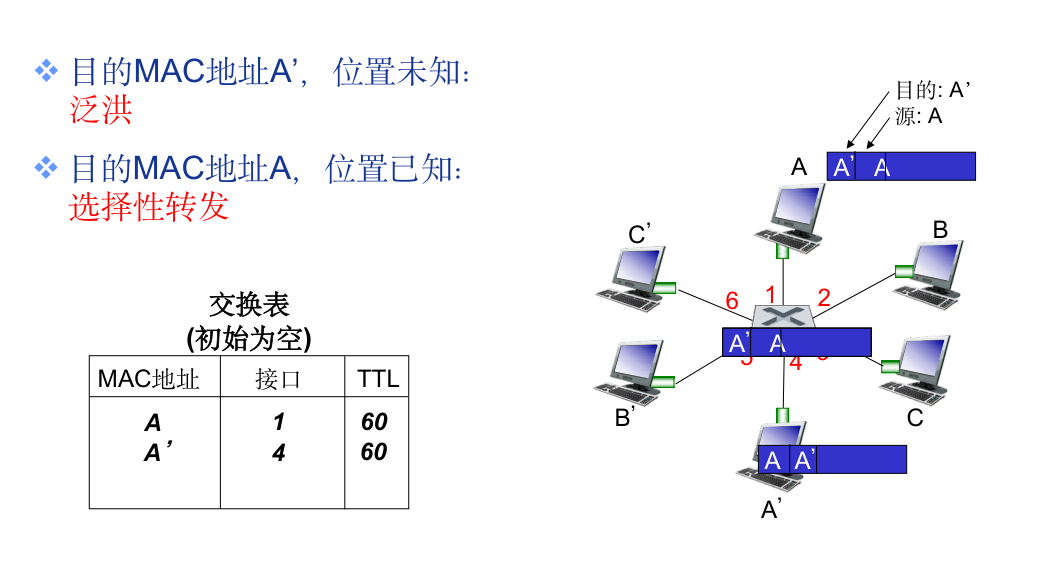
\includegraphics[width=0.86\textwidth]{ch03-switch-learning.png}
 \caption{首次目的地址未知时泛洪；交换机学习源地址后，返回帧可按表选择性转发。来源：\texttt{Chapter3-数据链路层.pdf}，PDF 第 118 页（显示页 118），局部截取。}
 \label{fig:ch03-switch-learning}
\end{figure}

\annotationarea{4}

\subsection{多交换机自学习例题}
\textbf{课件例题（PDF p.120）。} 拓扑中，交换机 $S_1$ 接主机 A、B、C 并连接 $S_4$；$S_2$ 接 D、E、F 并连接 $S_4$；$S_3$ 接 G、H、I 并连接 $S_4$。四台交换机的表初始为空。C 向 H 发帧，H 随后向 C 回应。求各交换机表项并说明转发过程。

\textbf{解：}
\begin{enumerate}
 \item C 的帧到 $S_1$。$S_1$ 学习 $C\to C$ 所连端口；H 未知，于是向 A、B、$S_4$ 方向泛洪。
 \item 帧到 $S_4$。$S_4$ 学习 $C\to S_1$；H 未知，向 $S_2$ 和 $S_3$ 方向泛洪。
 \item $S_2$、$S_3$ 分别学习 $C\to S_4$。两台交换机均未知 H，于是分别向本地终端端口泛洪；H 收到帧。
 \item H 回帧到 $S_3$。$S_3$ 学习 $H\to H$ 所连端口，查表知 C 在 $S_4$ 方向，只向 $S_4$ 转发。
 \item $S_4$ 学习 $H\to S_3$，查 C 在 $S_1$ 方向，只向 $S_1$ 转发。
 \item $S_1$ 学习 $H\to S_4$，查 C 在本地端口，只向 C 转发。$S_2$ 未收到回应帧，不会由该次通信学到 H。
\end{enumerate}

通信完成后，相关交换表至少含有：$S_1$：C 到本地 C 端口、H 到 $S_4$；$S_2$：C 到 $S_4$；$S_3$：C 到 $S_4$、H 到本地 H 端口；$S_4$：C 到 $S_1$、H 到 $S_3$。端口号按拓扑端口表示，没有从课件图中标出的端口编号处用相邻主机或交换机名称表示。

\annotationarea{4}

\subsection{Hub、交换机与冲突域}
\textbf{集线器（Hub）}工作在物理层，只再生或复制比特，不读取 MAC 地址。它不会隔离冲突域，也不会隔离广播域。\textbf{交换机和网桥}工作在数据链路层，能按帧地址过滤或转发，从而隔离冲突域，但普通二层交换机不会隔离广播域。路由器在网络层转发不同网络间的分组，通常构成广播域边界。

课件对设备的对照还列出即插即用、优化路由和直通传输：Hub、交换机、网桥均标为即插即用，不负责优化路由；直通传输是读出目的地址后即可开始转发，不等待完整帧到齐。采用存储转发时，交换机先接收完整帧并检查 FCS，再作转发决定。交换机端口专用、全双工时可支持多对端口并行通信；连接共享式 Hub 的端口仍按共享段规则工作。

\annotationarea{4}

\subsection{VLAN 与 IEEE 802.1Q}
单一大型广播域中的地址解析协议（Address Resolution Protocol，ARP）、动态主机配置协议（Dynamic Host Configuration Protocol，DHCP）和未知目的帧会到达较多链路，也带来管理、效率、隐私和隔离问题。\textbf{虚拟局域网（Virtual Local Area Network，VLAN）}将一个物理交换网络划分成多个逻辑广播域。主机更换物理位置后，若希望逻辑上仍属于原部门，可以通过 VLAN 成员配置保持其逻辑归属。

课件列出基于端口、MAC 地址、协议和子网的 VLAN 划分方法。端口 VLAN 最直观：把若干交换机端口分到同一 VLAN；端口可以按管理配置动态分配。不同 VLAN 之间不能直接进行二层通信；需要通过路由器或具有三层转发功能的交换机转发。

同一 VLAN 若跨越多台交换机，交换机之间的\textbf{中继端口（trunk port）}可以承载多个 VLAN 的帧。接入端口按本地配置识别 VLAN；帧通过 trunk 时需携带 VLAN 标识。

\textbf{IEEE 802.1Q}在以太网帧的源地址字段之后、类型字段之前插入 4 B VLAN 标记。其前 2 B 是标记协议标识符，值为 \texttt{0x8100}；后 2 B 的标记控制信息含 3 bit 优先级、1 bit 规范格式指示符（Canonical Format Indicator，CFI）和 12 bit VLAN 标识符（VLAN Identifier，VID）。VID 标识该帧所属的 VLAN。无标记帧为普通以太网帧；带标记帧用于交换机间携带 VLAN 信息。标签插入后 FCS 应按新帧内容计算。

\textbf{跨交换机转发例：}主机接入端口属于 VLAN 10，向另一台交换机上的 VLAN 10 主机发送帧。入口交换机按端口配置识别 VLAN 10，在 trunk 发出时插入 VID=10；出口交换机据 VID 只在 VLAN 10 内转发，并在向普通未标记接入口送出时去掉标签。VLAN 20 的端口不接收该帧。课件显示的最大数据载荷为 1500 B，插入 4 B 标记后最大帧长由 1518 B 增至 1522 B。

\begin{figure}[H]
 \centering
 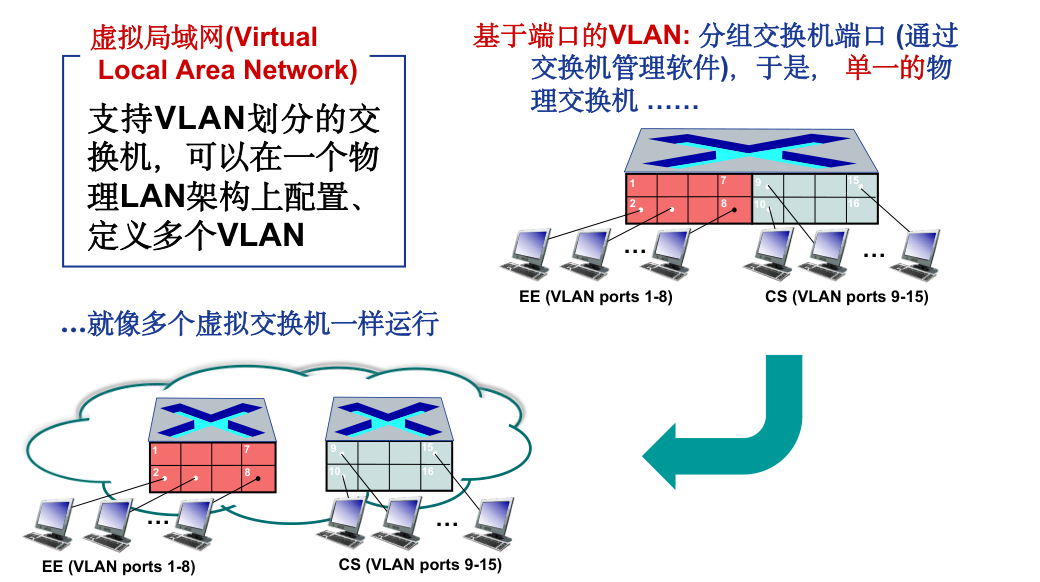
\includegraphics[width=0.86\textwidth]{ch03-vlan.png}
 \caption{同一物理交换网络被配置为多个逻辑 VLAN；广播只在相应 VLAN 内传播。来源：\texttt{Chapter3-数据链路层.pdf}，PDF 第 127 页（显示页 127），局部截取。}
 \label{fig:ch03-vlan}
\end{figure}

\annotationarea{4}

\begin{quote}\small 来源：课件 PDF 第 96--131 页（显示页 96--131）；参考书 §3.6，PDF 第 98--123 页（印刷第 87--112 页）及 §3.8，PDF 第 128--136 页（印刷第 117--125 页）。课件例题：交换机自学习第 118 页、多交换机转发第 120 页。课件第 105 页的 512 $\mu$s 与其 512 bit / 10 Mb/s 不一致，按计算结果订正为 51.2 $\mu$s。\end{quote}

\section{PPP 协议}

\subsection{点对点链路和 PPP 的设计需求}
\textbf{点对点链路}只有一个发送端和一个接收端，例如拨号或专线连接；与广播链路相比，不需要多个结点竞争信道，也不需要使用 MAC 地址从多个接收者中选择目的接口。课件列出高级数据链路控制（High-Level Data Link Control，HDLC）和点对点协议（Point-to-Point Protocol，PPP）两种点对点数据链路控制协议，本节重点讲 PPP。

\textbf{点对点协议（PPP，Point-to-Point Protocol）}由互联网工程任务组（Internet Engineering Task Force，IETF）制定，可在不同链路上运行，也可承载不同网络层协议。PPP 的设计需求包括：组帧并支持多种网络层载荷；对任意比特模式提供透明传输；检测差错；检测连接是否仍然活动并向网络层报告链路状态；协商网络层地址或相关配置。

PPP 不需支持差错纠正与恢复、流量控制、乱序交付或多点链路。差错恢复等功能可由高层协议处理。PPP 对帧作差错检测，但在数据传输期间不使用逐帧序号和 ACK 来恢复错误帧；因此，链路建立阶段存在控制协商，不代表每个数据帧均可靠交付。

\annotationarea{4}

\subsection{PPP 帧字段}
常见 PPP 帧由首尾标志字段、地址、控制、协议、信息和 FCS 组成。课件图示的常见未压缩格式为：
\begin{center}
\begin{tabularx}{0.98\textwidth}{l l X}
\toprule
字段 & 常见长度与值 & 作用\\
\midrule
Flag & 1 B，\texttt{0x7E} & 帧定界符，首尾各一个\\
Address & 1 B，\texttt{0xFF} & PPP 常见固定值，不是以太网目的 MAC\\
Control & 1 B，\texttt{0x03} & PPP 常见固定值\\
Protocol & 2 B & 标识信息字段的上层协议或控制协议\\
Information & 0--1500 B & 网络层数据报或 PPP 控制报文\\
FCS & 通常 2 B，也可为 4 B & CRC 差错检测字段\\
Flag & 1 B，\texttt{0x7E} & 帧结束定界符\\
\bottomrule
\end{tabularx}
\end{center}
课件把 Address、Control 描述为无效或暂未定义的字段。PPP 是点对点链路，不依靠它们作多站地址选择。PPP 不用 CSMA/CD，不需要以太网的 64 B 最小帧限制。

\begin{figure}[H]
 \centering
 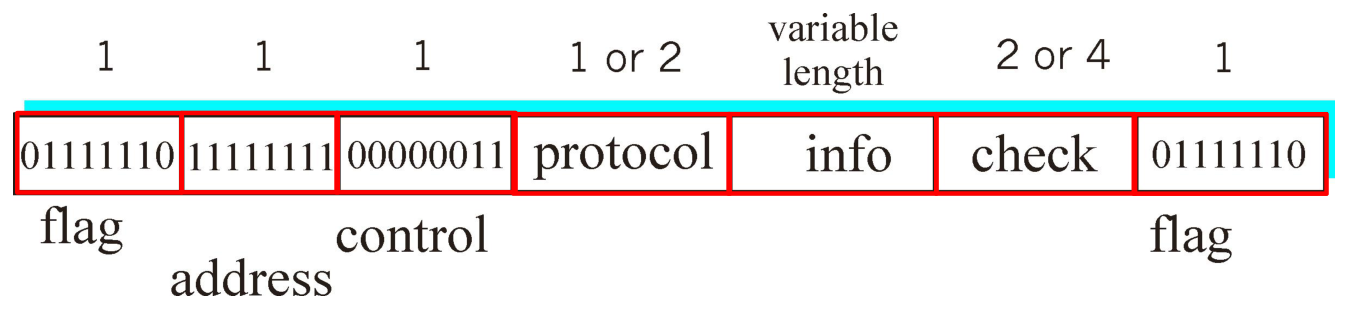
\includegraphics[width=0.94\textwidth]{ch03-ppp-frame-detail.png}
 \caption{PPP 帧字段及常见长度；Protocol 字段说明信息字段的协议类型。来源：\texttt{Chapter3-数据链路层.pdf}，PDF 第 137 页（显示页 137），局部截取。}
 \label{fig:ch03-ppp-frame}
\end{figure}

\annotationarea{4}

\subsection{PPP 的字节填充和零比特填充}
帧首尾使用 \texttt{0x7E} 定界，信息字段仍可能包含相同模式。PPP 按链路传输方式选择填充方法。

\textbf{异步传输：字节填充。} 转义字节为 \texttt{0x7D}。信息字段中的 \texttt{0x7E} 转为 \texttt{0x7D 0x5E}，\texttt{0x7D} 转为 \texttt{0x7D 0x5D}；原字节值和 \texttt{0x20} 做异或。数值小于 \texttt{0x20} 的控制字符也按规则转义，例如 \texttt{0x03} 变为 \texttt{0x7D 0x23}，\texttt{0x11} 变为 \texttt{0x7D 0x31}，\texttt{0x13} 变为 \texttt{0x7D 0x33}；课件还列出奇偶位为 1 的 \texttt{0x91} 和 \texttt{0x93}，分别变为 \texttt{0x7D 0xB1}、\texttt{0x7D 0xB3}。接收端去掉转义字节，并对转义后的值再次与 \texttt{0x20} 异或，恢复原字节。

\textbf{同步传输：零比特填充。} 帧内每连续出现 5 个 1 后插入 0；接收端删除连续 5 个 1 后的填充 0。该规则确保帧内数据不会冒充边界 \texttt{01111110}。

\annotationarea{4}

\subsection{LCP、认证、NCP 与 PPPoE}
在交换网络层数据前，两端需配置 PPP 链路并取得网络层所需信息。链路控制协议（Link Control Protocol，LCP）用于建立、配置和检测链路，也可协商最大帧长、认证等选项；若配置了认证，认证成功或双方不要求认证后继续；网络控制协议（Network Control Protocol，NCP）再配置所承载网络层协议的信息，例如 IP 地址。

课件第 141 页提到 IP 控制协议（IP Control Protocol，IPCP）报文用于配置 IP 信息，并把数值 8021 写成“IP 分组首部的上层协议字段”。这里应归属于\textbf{PPP 帧的 Protocol 字段}，且是十六进制 \texttt{0x8021}。参考书列出的常见值为：\texttt{0xC021} 表示 LCP，\texttt{0x8021} 表示 IPCP，\texttt{0x0021} 表示 IPv4 数据报。IPCP 与 IPv4 数据报因此不是同一类载荷。

\textbf{PPPoE（PPP over Ethernet）}把 PPP 会话承载在以太网链路上，常见于宽带接入。课件给出两种组网方式：机构网关作为一个 PPPoE 客户端，内部主机共享一个 PPP 会话；或者每台主机分别运行客户端，与运营商接入服务器各自建立会话。

课件将 PPPoE 工作过程分为三阶段：\textbf{Discovery} 获取对端以太网地址并确定会话 ID；\textbf{Session} 进行 PPP 协商并传输 PPP 数据；\textbf{Terminate} 发送报文结束会话。课件第 143 页将认证、加密和压缩并列为 PPPoE 能力；参考书对应内容主要说明 PPP 可协商认证、进行访问控制和计费。本笔记保留课件的接入场景，同时不把加密视为 PPP 帧或会话本身自动提供的属性。

\annotationarea{4}

\begin{quote}\small 来源：课件 PDF 第 132--146 页（显示页 132--146）；参考书 §3.7.2，PDF 第 125--126 页（印刷第 114--115 页）。课件第 141 页将 IPCP 的 \texttt{0x8021} 误称为 IP 首部字段；应为 PPP Protocol 字段。\end{quote}

\section{链路虚拟化}

\subsection{用 IP 屏蔽底层网络差异}
\textbf{虚拟化}是一种抽象方法：上层使用下层提供的统一接口，不必了解下层内部的每一个实现细节。课件用虚拟内存、虚拟设备等说明这种抽象，再将其用于网络。

互联网形成早期，不同网络有各自的寻址约定、分组格式、差错恢复和路由方法。课件列出的异构网络包括 ARPANET、电缆数据网络、ALOHA 卫星网络和分组无线网络。\par
IP 作为统一的网际层，为这些网络提供统一的网络层寻址和分组格式，使网络在网际层看起来较为一致；体系结构因此包含网际层地址和本地网络地址两层寻址。课件中的\textbf{网关（gateway）}把网际层分组封装进本地网络的分组格式，或从本地分组中取出网际层分组，再沿网际层路由到下一网关。

底层电缆、卫星、电话调制解调器等网络技术由各自的链路机制实现；异步传输模式（Asynchronous Transfer Mode，ATM）和多协议标签交换（Multiprotocol Label Switching，MPLS）等网络从 IP 路由器的视角可表现为连接两个 IP 路由器的逻辑链路。统一的 IP 层并不意味着底层网络使用相同帧格式或相同物理介质，而是通过逐层封装和接口抽象隐藏差异。

\begin{quote}\small 来源：\texttt{Chapter3-数据链路层.pdf}，PDF 第 147--152 页（显示页 147--152）。课件以 Cerf 与 Kahn 的互联网体系结构说明不同底层网络如何由统一的网际层连接；参考书第 3 章未设置完全对应的小节。\end{quote}
\annotationarea{2}

% 第4章：课程课件与教材核对后整理；图示来源见 Book/page_index.md。
\chapter{网络层}
\noindent\textbf{本章要解决的问题。} 第3章解决相邻结点之间怎样传递帧；网络层解决怎样把分组跨过多个不同网络，从源主机送到目的主机。为此，网络层需要地址、转发表以及建立转发表的路由协议；还要处理分组过大、地址配置和差错报告等问题。本章依照课件顺序展开。

\small 本章来源页码写作“PDF阅读器页（课件显示页）”；两者相同时只列一个页码。教材页码均注明PDF页和印刷页，不能互换。\normalsize

\section{网络层服务}
\subsection{转发、路由与服务模型}
主机发送时将传输层的报文段等数据封装为\textbf{IP数据报}，经过多个路由器，到达目的主机后交给相应上层协议。路由器通常不需要知道应用内容，而依据分组首部及转发表决定如何处理。网络层的工作可分为\textbf{数据平面}和\textbf{控制平面}：数据平面逐个处理数据报，控制平面决定各路由器应使用哪些转发表项。传统路由协议由多个路由器协同计算；课件也简要介绍由控制器集中计算规则的SDN思路。

\textbf{转发（forwarding）}是单个路由器收到分组后，将其从输入接口送往合适输出接口的动作；\textbf{路由选择（routing）}是根据拓扑和规则确定到达目的网络的路径、形成路由信息的过程。可把前者理解成路口按路牌选择出口，后者是如何确定和更新路牌。路由表侧重路径计算，转发表是为高速查找整理出的结果；简化讨论时两者常统称路由表。

互联网的网络层通常提供\textbf{无连接、尽力而为}的数据报服务：发送前不由网络层为该数据流建立连接，网络尽力传递但不保证送达、按序、无重复或特定时延。若应用需要可靠交付，可由 TCP 等上层机制提供。网络层服务是主机到主机；传输层面向应用进程，TCP 的连接由端系统维护，并不要求中间路由器建立 TCP 连接状态。

\subsection{拥塞及其代价}
\textbf{拥塞}指注入网络的流量超过某些链路或设备的处理能力。有限缓存排满会丢包；即使缓存很大，等待时间也会增长。发送方重传会占用更多链路能力；一包已走过多跳后才丢失，之前各跳消耗的资源也不能收回。拥塞控制关注整个网络的负荷，\textbf{流量控制}主要防止某个接收方来不及接收，两者目的不同。

拥塞可以由端系统根据丢包、时延等迹象推测，也可以由网络设备显式反馈。课件介绍的网络辅助手段包括流量感知路由、准入控制、调节发送流量与过载时主动丢弃；ATM ABR 服务使用资源管理信元反馈拥塞或可用速率。这些是不同体系的机制，不代表 IP 本身承诺固定速率。\par\small\noindent 来源：第4章课件 PDF 第4--18页；参考书 PDF 第138--143页（印刷第127--132页）。\normalsize

\annotationarea[4]
\section{虚电路网络与数据报网络}
\textbf{虚电路（VC）}是分组交换网络中的逻辑路径。典型过程为建立、沿路径传输、拆除；建立时路径上的设备保存状态。一个分组携带本段链路有效的虚电路号 VCID，路由器用“输入接口、输入 VCID”查表，得到“输出接口、输出 VCID”，然后替换编号。不同链路上同一虚电路的编号可以不同；它仍共享物理链路，不等于独占电路，是否预留带宽及可靠性取决于具体服务。

\begin{figure}[H]\centering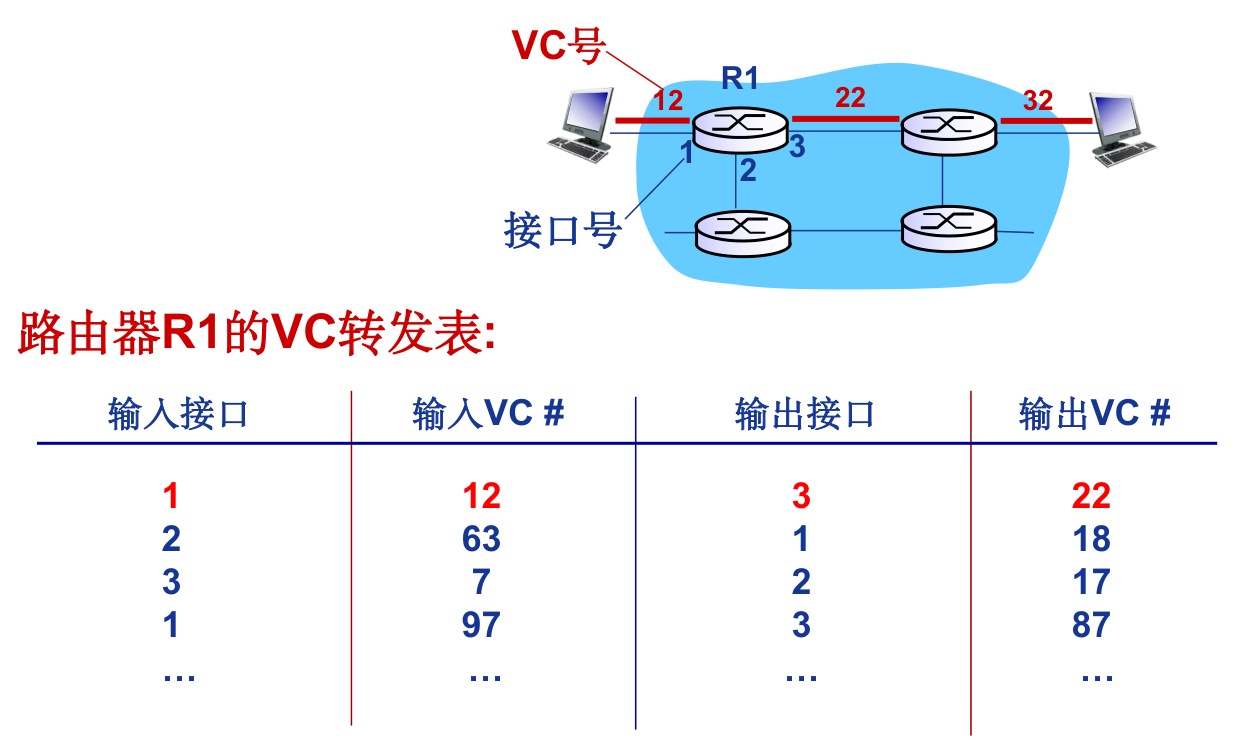
\includegraphics[width=.83\textwidth]{ch04-vc-table.png}\caption{虚电路转发表：输入接口1、编号12对应输出接口3、编号22。来源：Chapter4-网络层.pdf，PDF第24页（显示页24），局部截取。}\end{figure}

\textbf{数据报网络}不为一串数据报预先建立网络层连接。每个分组携带目的地址，路由器对它独立查表；在路由变化时同一应用的分组可能走不同路径。不同路径、排队和丢包都可能使分组失序。与 VC 不同，普通 IP 路由器不按每个用户会话保存连接状态。

\textbf{最长前缀匹配。} 前缀是地址的前若干位。若目的地址同时匹配多条路由，选共同前缀最长的一条；例如 \texttt{200.23.24.5} 同时匹配 \texttt{200.23.0.0/16} 和 \texttt{200.23.24.0/24}，选择后者。默认路由 \texttt{0.0.0.0/0} 只有在没有更具体匹配时使用。若既无匹配又无默认路由，则无法按表继续转发。
\par\small\noindent 来源：课件 PDF 第20--33页；教材 PDF 第140--142页（印刷第129--131页）。\normalsize

\annotationarea[4]
\section{路由器体系结构}
路由器包括运行路由协议、管理路由信息的\textbf{路由处理器}，以及高速处理分组的输入端口、\textbf{交换结构}和输出端口。输入端口接收信号、处理链路层帧、查询转发表；交换结构把分组移向对应输出；输出端口排队、选择发送顺序，重新封装并送往下一条链路。
\begin{figure}[H]\centering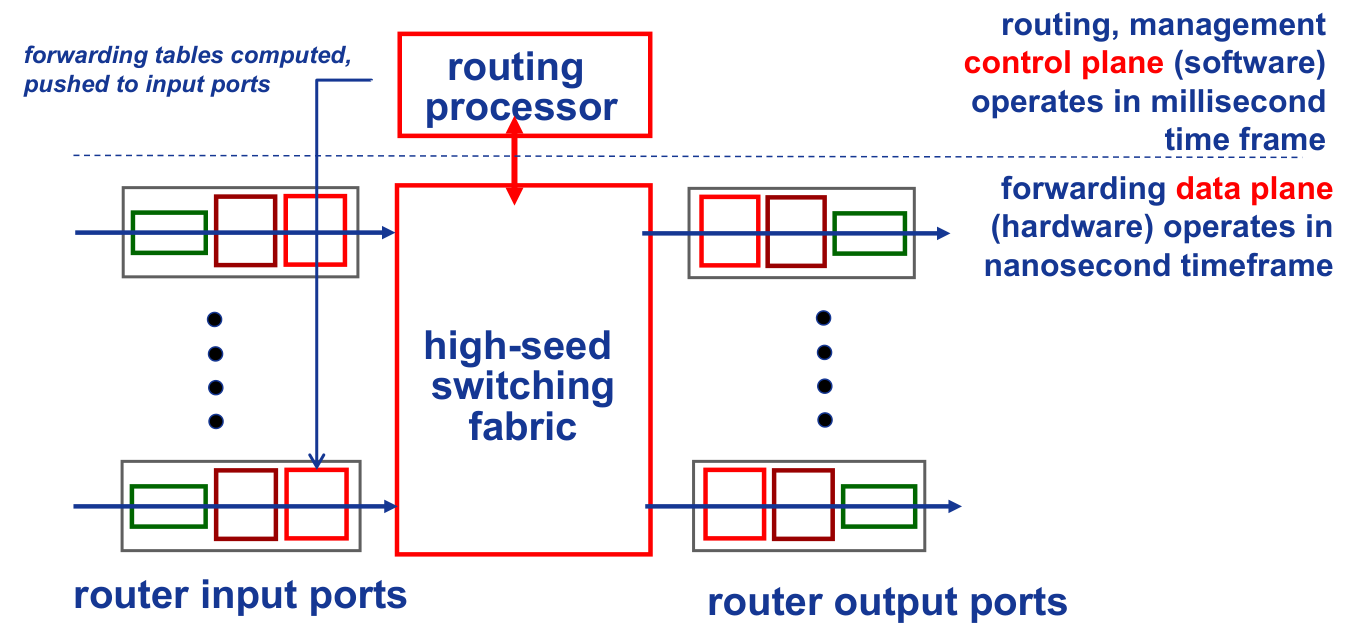
\includegraphics[width=.8\textwidth]{ch04-router.png}\caption{路由器内部：左侧输入端口经交换结构连接右侧输出端口，处理器提供转发所需的表。来源：Chapter4-网络层.pdf，PDF第35页（显示页35），局部截取。}\end{figure}
交换结构可以通过共享内存、共享总线或互连网络实现；前两者受共享带宽制约，交叉开关等互连结构可允许不同输入到不同输出并行。输入到达速率高于交换结构处理能力时，输入处排队；队首分组争不到输出而阻挡后面本可发送的分组，称\textbf{队首阻塞}。若多个输入同时汇聚到同一输出，输出链路来不及发送也会排队，缓存满则丢包。

\textbf{调度}决定等待分组的发送顺序：FIFO 先到先服务；优先级调度先选高优先级，低优先级可能长期等待；轮询依次服务各类队列；加权公平排队按权重分配服务，所有队列持续有待发数据时，可近似按权重分享链路，实际分组长度会影响瞬时顺序。课件给出的按带宽与 RTT 估算缓存容量是经验模型，适用前提决定其结果，不能当成固定标准。\par\small\noindent 来源：课件 PDF 第35--51页；教材 PDF 第225--227页（印刷第214--216页）。\normalsize

\annotationarea[4]
\section{IP协议}
\subsection{IPv4首部与逐跳处理}
IPv4 地址长32位，写作四个0--255的十进制数，例如 \texttt{192.168.1.10}。数据报由首部和数据组成；首部至少20字节，携带目的地址和各项处理信息。
\begin{figure}[H]\centering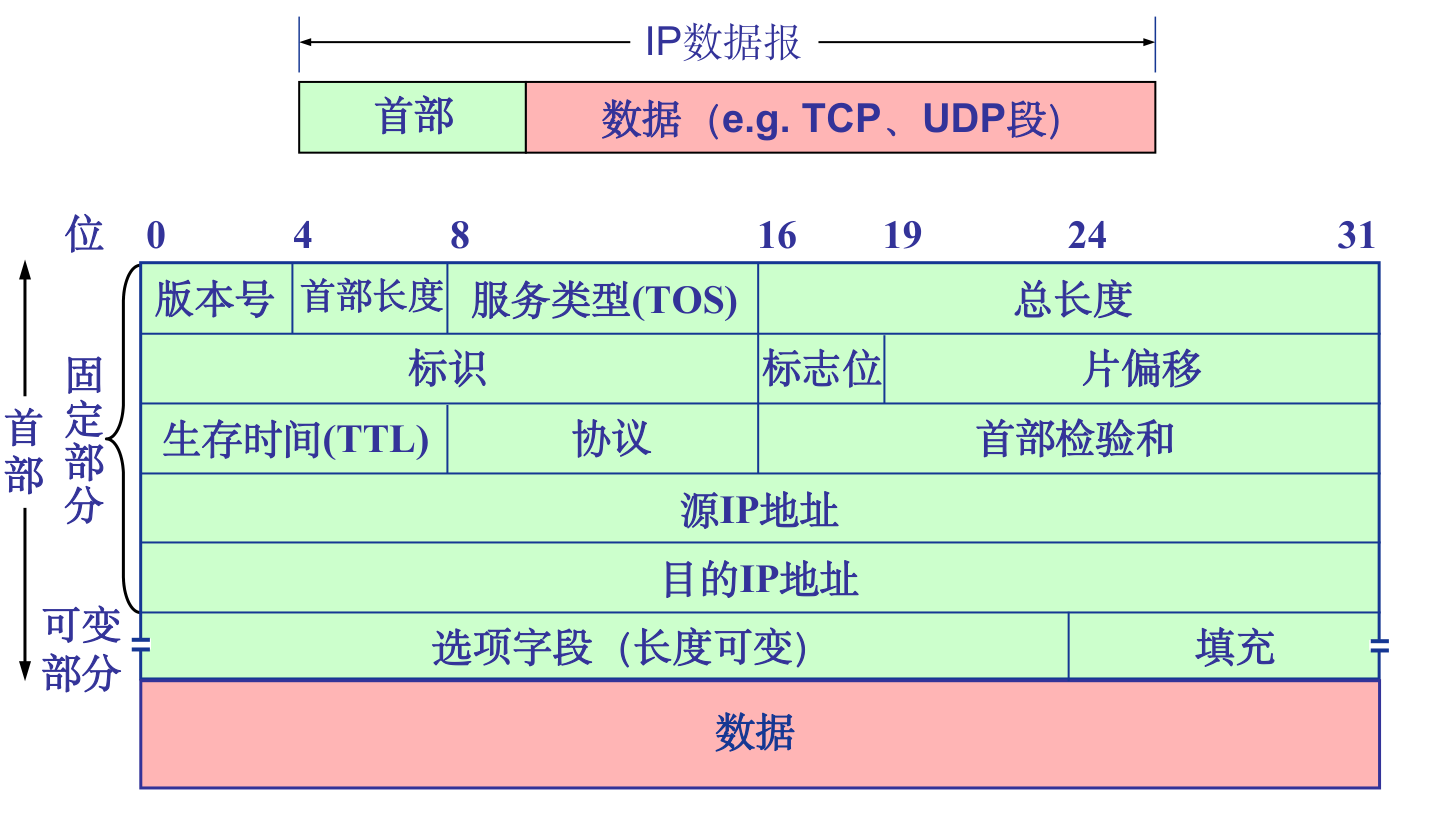
\includegraphics[width=.83\textwidth]{ch04-ipv4-header.png}\caption{IPv4数据报首部与载荷；横向字段宽度之和每行为32位。来源：Chapter4-网络层.pdf，PDF第54页（显示页54），局部截取。}\end{figure}
\begin{itemize}[nosep]
\item \textbf{版本}4位，IPv4取4；\textbf{首部长度 IHL}4位，以4字节为单位，因此值5表示20字节，最大值15表示60字节。选项使首部可变长，填充用于4字节对齐。
\item \textbf{服务类型}8位，现代解释包括DSCP和ECN；\textbf{总长度}16位，以字节计，包含首部和载荷，最大65535字节。
\item \textbf{标识}16位；\textbf{标志}3位；\textbf{片偏移}13位。DF=1表示不允许分片；MF=1表示后面还有分片；片偏移单位为8字节。
\item \textbf{生存时间 TTL}8位，在每个转发路由器递减，减至0则丢弃以限制环路；\textbf{协议}8位，指出载荷交给哪种上层协议，如ICMP=1、TCP=6、UDP=17。
\item \textbf{首部校验和}16位，只检验IPv4首部，不检验载荷；TTL等字段改变时须更新。源、目的IP各32位；普通路由转发通常不改它们，NAT等特殊处理会改写。
\end{itemize}

\subsection{MTU与IPv4分片}
\textbf{最大传输单元（MTU）}是当前链路能够承载的最大IP数据报长度，含IP首部而不含链路帧首尾。若数据报长于输出链路MTU，IPv4路由器在DF=0时可以分片；DF=1则丢弃并可返回相应ICMP差错。片由目的主机重组，一个片丢失会使原数据报无法完整重组。

\textbf{课件例：}原报总长4000字节，首部20字节，无选项，MTU=1500字节。原载荷 $4000-20=3980$ 字节；前两片载荷各1480字节，均为8的倍数；余下 $3980-2960=1020$ 字节。每片都要重新拥有20字节首部：
\begin{center}\begin{tabular}{cccc}\toprule 片 & 总长（字节） & MF & 片偏移（8字节）\\\midrule 1 &1500&1&0\\2&1500&1&185\\3&1040&0&370\\\bottomrule\end{tabular}\end{center}
片偏移是相对于\emph{原数据载荷起点}，例如第二片从第1480字节开始，所以偏移为 $1480/8=185$；所有片标识相同。除最后一片外，载荷长度须为8的倍数。若首部长度或选项复制情况不同，应按各片实际首部重新计算，不能机械套用20字节。若已经是分片的数据报再次分片，新片偏移须在原片偏移基础上计算；原片MF为1时，产生的最后一小片也仍须标记MF=1。
\begin{figure}[H]\centering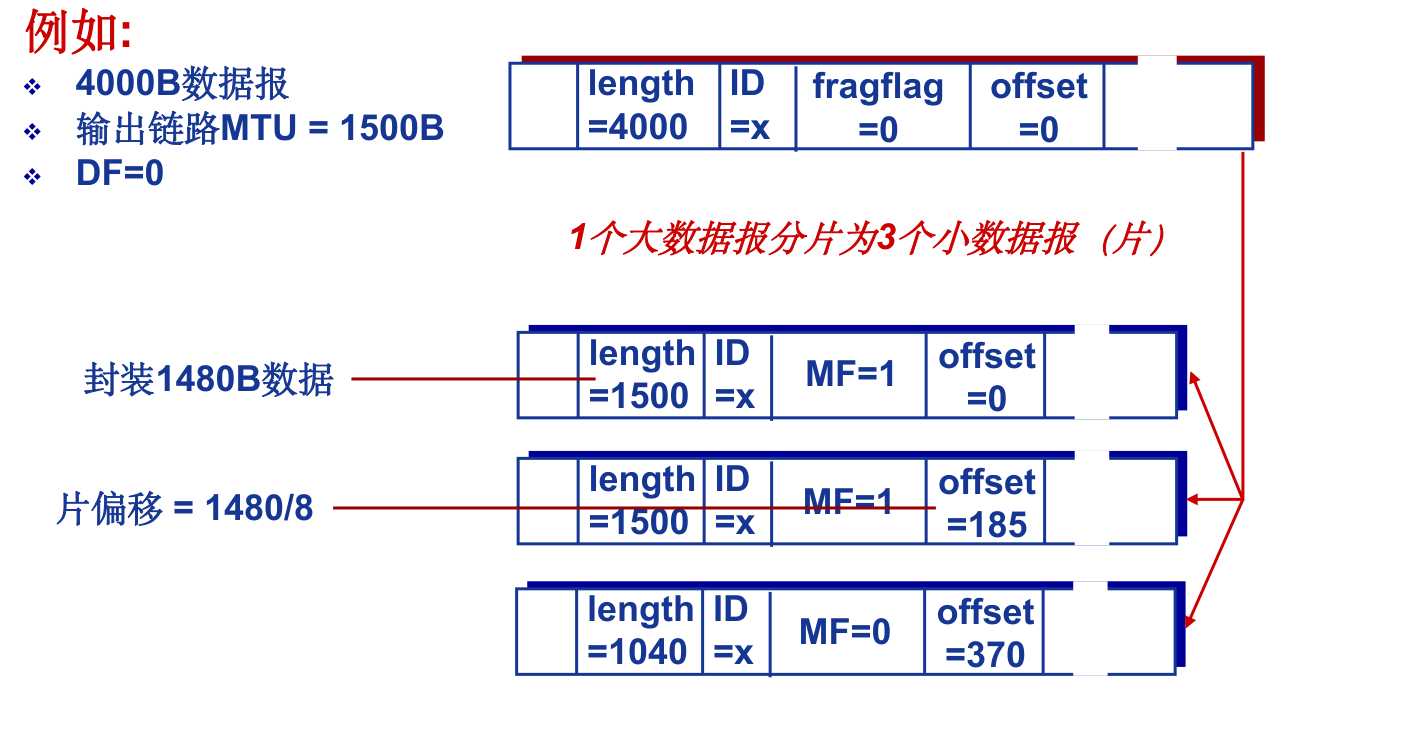
\includegraphics[width=.86\textwidth]{ch04-fragments.png}\caption{4000字节IPv4数据报的分片过程；箭头表示由原报产生三个独立IP分片。来源：Chapter4-网络层.pdf，PDF第72页（显示页72），局部截取。}\end{figure}

\subsection{地址、子网、掩码与无类编址}
IP地址通常配置在接口上，路由器连接多条网络，因而各接口可有不同地址。子网中地址高位的\textbf{网络前缀}相同，低位区分接口；路由器借前缀找到目标网络。\textbf{掩码}是前缀位为1、余下为0的32位数，地址与掩码逐位做 AND，得到网络地址。\texttt{/23} 表示前23位为前缀，即掩码 \texttt{255.255.254.0}。

\begin{sloppypar}
\textbf{课件例：}地址 \texttt{172.32.1.112/23} 中第三字节 $1=00000001_2$，掩码第三字节 $254=11111110_2$；与运算为0，因此网络为 \texttt{172.32.0.0/23}。主机部分9位，地址共 $2^9=512$ 个：从 \texttt{172.32.0.0} 到 \texttt{172.32.1.255}。对于普通广播子网，首地址表示网络、末地址为定向广播地址，可分配范围为 \texttt{172.32.0.1} 至\allowbreak \texttt{172.32.1.254}，共510个。点到点 /31 与主机路由 /32 有特殊用途，不能套用减2公式。
\end{sloppypar}

历史上的A、B、C类默认前缀分别为8、16、24位；D类用于多播，E类保留。A类0和127等范围有特殊用途，不能简单认为每个地址都可作普通主机地址。现在常用\textbf{无类域间路由 CIDR}，用地址加前缀长度指明范围；私有地址为 \texttt{10.0.0.0/8}、\texttt{172.16.0.0/12}、\texttt{192.168.0.0/16}，不应在公共互联网按普通公网地址转发。

\textbf{课件划分例：}将 \texttt{192.168.1.0/24} 中已分配的 \texttt{192.168.1.0/25} 留出后，剩余 \texttt{192.168.1.128/25} 划分给需要60、30、30个地址的三个局域网。先分最大需求：/26有64个地址、62个可分配；两个/27各有32个地址、30个可分配：
\begin{center}\begin{tabular}{llll}\toprule 前缀 & 可用地址范围 & 广播地址 & 可用数\\\midrule
192.168.1.128/26 & .129--.190 & .191 & 62\\
192.168.1.192/27 & .193--.222 & .223 & 30\\
192.168.1.224/27 & .225--.254 & .255 & 30\\\bottomrule\end{tabular}\end{center}
表中简写的末字节均属于 \texttt{192.168.1}。分配地址应先选能容纳需求的最小块，并按块边界对齐，确认各块不重叠。

\begin{sloppypar}
\textbf{路由聚合}用一个共同前缀概括多个目的网络，缩小路由表。例如相邻的\allowbreak \texttt{202.118.1.0/25} 与\allowbreak \texttt{202.118.1.128/25} 都从同一下一跳可达，可聚合为 \texttt{202.118.1.0/24}。聚合后须检查所有被涵盖地址都能正确转发，否则可能产生黑洞；更具体路由可通过最长前缀匹配覆盖汇总路由。
\end{sloppypar}

\subsection{IPv6与过渡}
IPv6使用128位地址，常写成8组十六进制数；每组前导零可省略，连续全零组可用一次 \texttt{::} 压缩，如 \texttt{FF01::43}。前缀仍用斜线长度表示，例如 \texttt{2002:43c:476b::/48}。单播是一对一，多播是一对多，任播将同一地址分配给一组接口并交付其中一个，通常按路由意义上的最近者选择。

IPv6基本首部固定40字节，有版本、流量类别、流标签、载荷长度、下一个首部、跳数限制、源与目的地址；扩展首部串联可选信息。基本首部没有IPv4首部校验和，路由器不执行IPv6分片；源节点可在需要时使用分片扩展首部。IPv6不使用IPv4式广播。\textbf{隧道}可将完整IPv6数据报装入IPv4载荷穿越IPv4网络，另一端解封装；内外层地址分别服务于原始通信和隧道两端。\par
\textbf{课件中的特殊IPv4地址：}
\begin{center}\small\setlength{\tabcolsep}{4pt}
\begin{tabularx}{\textwidth}{>{\raggedright\arraybackslash}p{5.8cm}>{\raggedright\arraybackslash}X}
\toprule 地址特征 & 课件所述用途\\\midrule
网络号全0、主机号全0 & 本网范围表示本机；在路由表中也可表示默认路由（需看使用场景）\\
网络号全0、主机号为特定值 & 表示本网内某个特定主机\\
网络号和主机号全1 & 本网广播地址，路由器不转发\\
特定网络号、主机号全0 & 网络地址，标识一个网络\\
特定网络号、主机号全1 & 该网络的直接广播地址\\
首字节为127、主机号非全0/全1 & 环回地址，用于本机软件测试\\\bottomrule
\end{tabularx}\end{center}
私有地址范围为\texttt{10.0.0.0/8}、\texttt{172.16.0.0/12}、\texttt{192.168.0.0/16}。\par\small\noindent 来源：课件 PDF 第53--113、201--208页；教材 PDF 第148--154、192--195页（印刷第137--143、181--184页）。\normalsize

\annotationarea[4]
\section{IP相关协议}
\subsection{ICMP、ping与traceroute}
\textbf{ICMP}（Internet控制报文协议）的报文装在IP数据报中，用于报告差错或网络探询，并不使IP传输自动可靠。例子有目的不可达、超时、重定向、回声请求和回声应答；课件所列源抑制是历史机制，不宜当成当前拥塞控制方案。

\textbf{ping}发送回声请求，收到回声应答可测往返时间；无应答可能是丢包或过滤，并不必然说明主机不存在。\textbf{traceroute}逐次发送TTL为1、2、3等的探测报文：第一跳将TTL减至0并可能返回ICMP超时，第二次由第二跳返回，以此推测路径。课件示例采用UDP探测，目的主机可用端口不可达响应终止；不同实现也可能用其他探测报文，路由或过滤变化会使结果不完整。通常不会针对ICMP差错报文再生成ICMP差错，也不会对非首个分片生成ICMP差错。

\subsection{DHCP：自动配置}
\textbf{动态主机配置协议 DHCP}让新加入的主机获得地址、子网掩码、默认网关、DNS服务器及租期。典型初始流程称DORA：
\begin{enumerate}[nosep]
\item 客户端广播 Discover 寻找服务器，尚无地址时源IP为 \texttt{0.0.0.0}；
\item 服务器返回 Offer，提出可用地址及租期；
\item 客户端广播 Request，表示选择某份提供；
\item 被选服务器返回 ACK 确认，客户端才使用配置；租期到期前可以续租。
\end{enumerate}
DHCP采用UDP，服务器端口67、客户端端口68。若服务器不在本广播域，可以通过DHCP中继转发请求；服务器响应不一定总是广播。默认网关是本子网上可转发到其他网络的路由器接口。

\annotationarea[3]
\subsection{NAT：多个内部主机共享外部地址}
\textbf{网络地址转换 NAT}可将内部私有地址与公网地址对应；课件例子同时转换传输层端口，这种多对一形式也称NAPT。主机 \texttt{10.0.0.1:3345} 访问 \texttt{128.119.40.186:80} 时，网关将源改为 \texttt{138.76.29.7:5001}，记录映射；回复以 \texttt{138.76.29.7:5001} 为目的到达网关后，再改回 \texttt{10.0.0.1:3345}。端口帮助区分内部会话，转换还涉及相关校验和更新。
\begin{figure}[H]\centering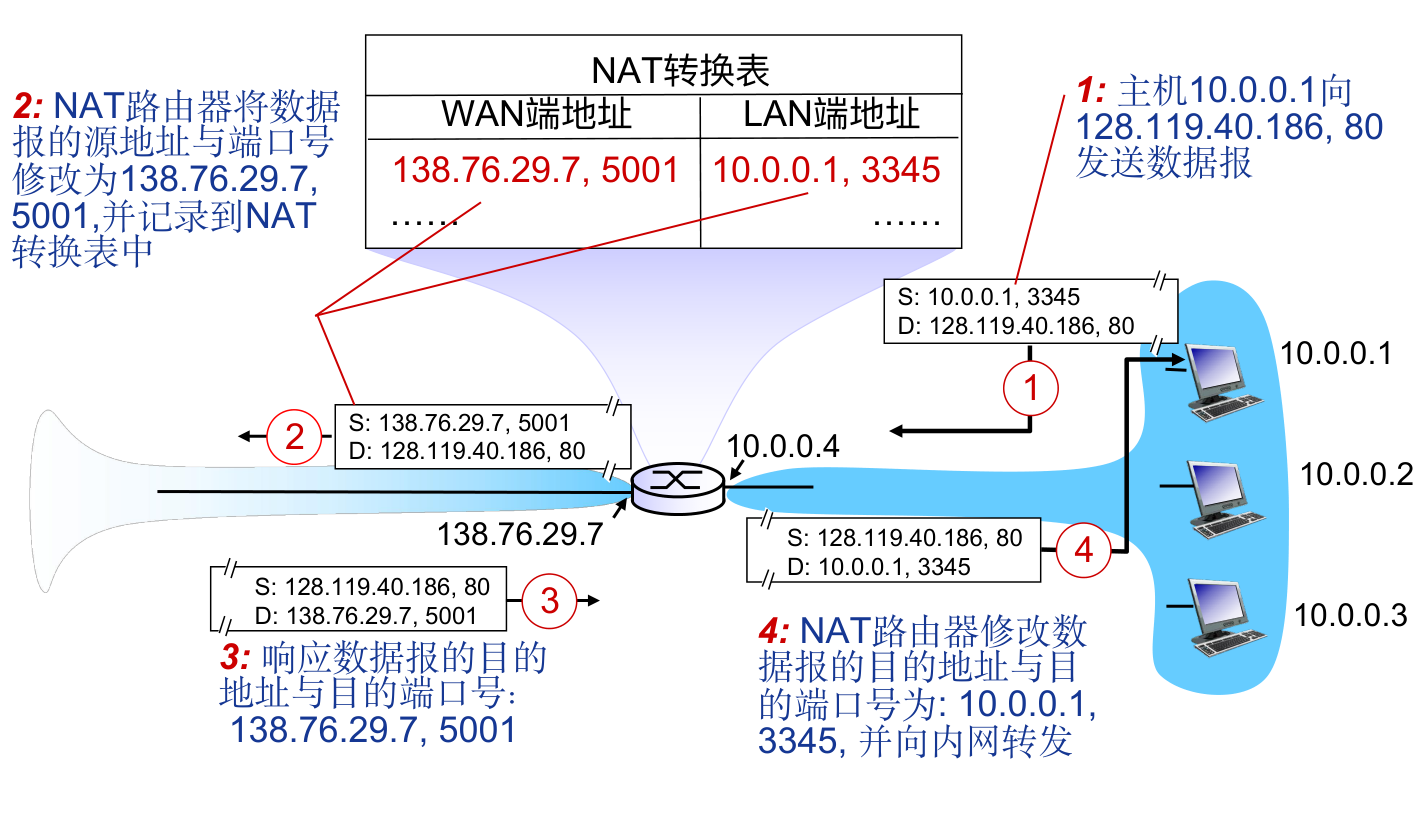
\includegraphics[width=.88\textwidth]{ch04-nat.png}\caption{NAT往返转换：编号1--4依次是请求、改写外出、回复和改写进入，表中记录地址与端口对应。来源：Chapter4-网络层.pdf，PDF第130页（显示页130），局部截取。}\end{figure}
外部主动访问内网服务器时，若没有对应映射，网关通常无法知道转给谁；可配置端口映射、通过网关控制协议建立映射，或使用中继。NAT改变端到端寻址，不等同于完整防火墙或安全保证。

\annotationarea[3]
\subsection{ARP与跨网段逐跳交付}
\textbf{地址解析协议 ARP}在本地链路上把下一跳IPv4地址解析成链路层MAC地址。A需要向同一局域网中的B发报而缓存无记录时，广播询问“谁拥有B的IP”；B通常单播应答其MAC，A缓存映射并设置有效期。ARP广播限制在本地广播域，不跨路由器查找远端主机。

若A与B不在同一子网，A查询到默认网关的IP，再用ARP解析\emph{网关接口}的MAC。第一跳帧的源MAC为A、目的MAC为网关；其中IP数据报源、目的仍为A、B。路由器去除旧帧、查表、解析下一跳并构造新帧；新帧中的MAC因链路而变，而普通转发中端到端IP不变，TTL递减。图中R左右接口各自连接一个网络，蓝色线表示对应链路，帧的目的MAC是本跳接收接口。
\begin{figure}[H]\centering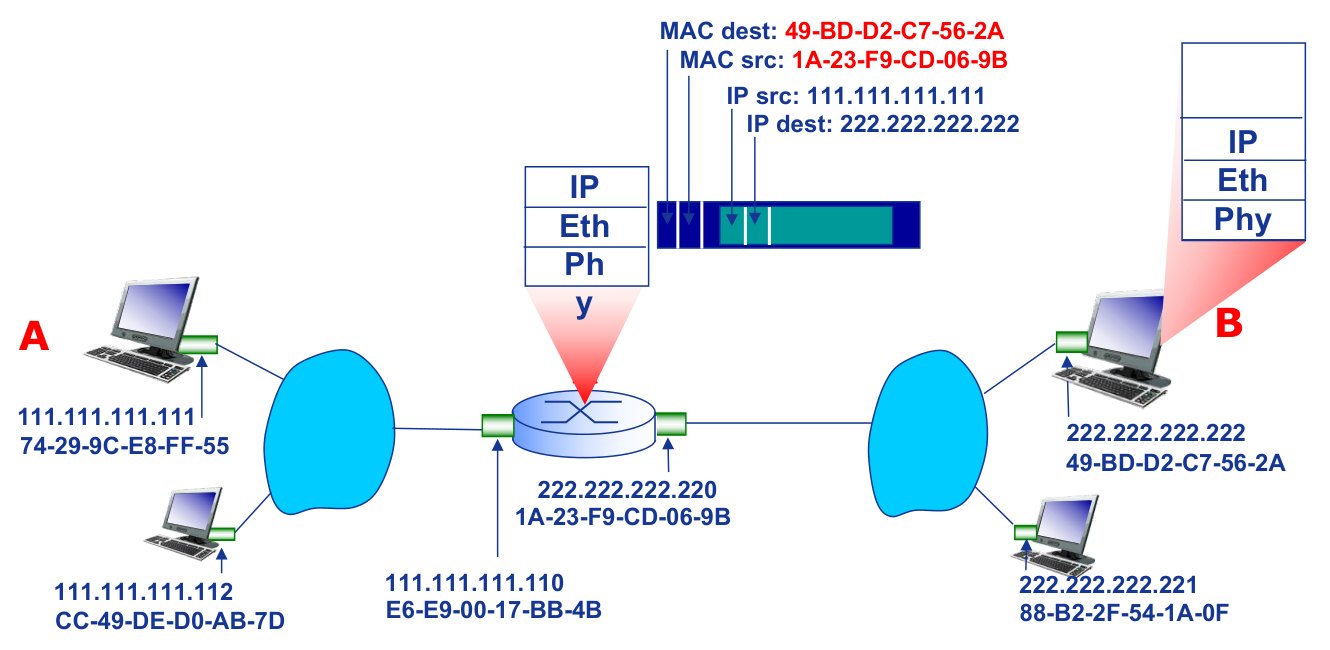
\includegraphics[width=.88\textwidth]{ch04-hop-addresses.png}\caption{跨两个局域网交付：路由器向右转发时，数据报目的IP仍为B，输出帧目的MAC换成B的MAC。来源：Chapter4-网络层.pdf，PDF第145页（显示页145），局部截取。}\end{figure}
\par\small\noindent 来源：课件 PDF 第115--146页；教材 PDF 第155--162页（印刷第144--151页）。\normalsize

\annotationarea[4]
\section{路由算法}
\subsection{图、费用和最短路径}
把路由器抽象为结点、链路抽象为边；链路费用 $c(x,y)$ 可表示跳数、配置的代价等。路径费用是各链路费用之和，\textbf{最短路径}即总费用最小，不一定是物理距离最短。静态路由由管理者配置，动态路由依据协议交换信息并更新；优先级取决于设备具体配置。

\subsection{链路状态与Dijkstra算法}
链路状态算法让路由器通告本地链路信息，参与者形成拓扑图，再各自计算到各目的地的最小费用路径。Dijkstra算法假设链路费用非负；记 $N'$ 为已确定最短费用的结点集，$D(v)$ 为源到结点 $v$ 的当前最好估计。初始化源结点加入 $N'$，其邻居估计设为直接链路费用，其他为无穷。然后重复：
\begin{enumerate}[nosep]
\item 在未确定结点中选 $D$ 最小的结点 $w$，加入 $N'$；
\item 对其未确定邻居 $v$，比较旧路径与经 $w$ 的路径，更新
\[D(v)\leftarrow\min\{D(v),\ D(w)+c(w,v)\};\]
\item 记录前驱，直到目标已确定或所有可达结点确定；沿前驱回溯即可找到源的下一跳。
\end{enumerate}
\textbf{课件图示例：}从 $u$ 出发，直接到 $w$ 的费用3、到 $x$ 为5、到 $v$ 为7。先确定 $w$，经 $w$ 可把 $v$ 改为 $3+3=6$；再确定 $x$，之后确定 $v$，经 $v$ 将 $y$ 更新为10；经 $y$ 将 $z$ 更新为12。表中每行表示已确定集合增长一次，$p(v)$ 是当前最优路径上的前驱。
\begin{figure}[H]\centering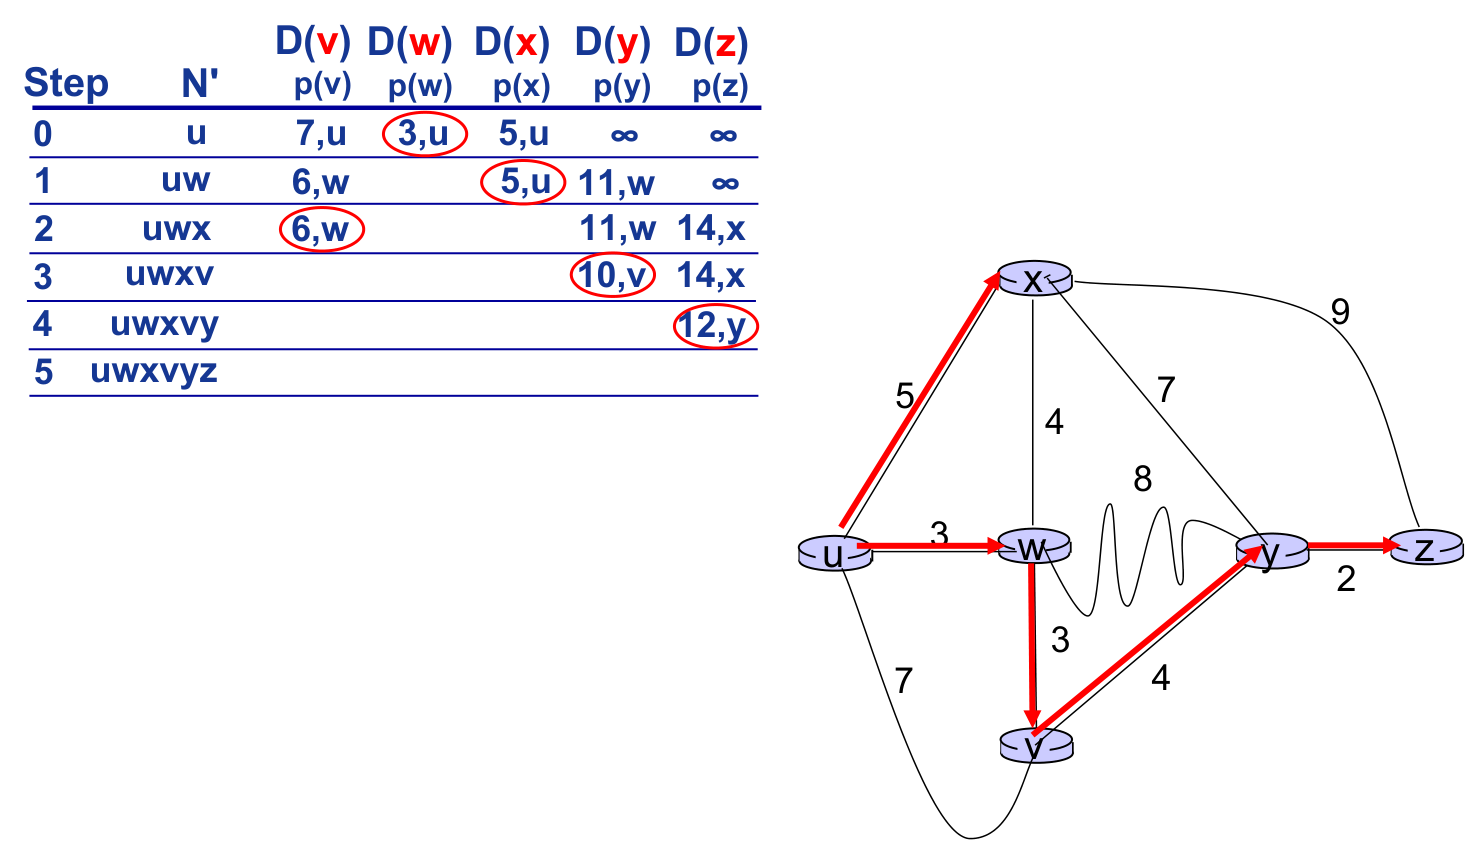
\includegraphics[width=.88\textwidth]{ch04-dijkstra.png}\caption{Dijkstra逐轮更新；左表记当前费用及前驱，右图中边上数字是费用。来源：Chapter4-网络层.pdf，PDF第155页（显示页155），局部截取。}\end{figure}
如果费用随流量改变且各路由器同步改路，负载可能在两条路径之间来回迁移，产生振荡。

\annotationarea[3]
\subsection{距离向量与无穷计数}
距离向量算法中，每个结点知道到邻居的链路费用，并向邻居通告自己到各目的地的距离估计。记 $D_x(y)$ 为结点 $x$ 估计到目的 $y$ 的费用，则收到邻居信息后更新
\[D_x(y)=\min_{v\text{为}x\text{的邻居}}\{c(x,v)+D_v(y)\}.\]
例如 $x$ 到 $y$ 为2、$y$ 到 $z$ 为1、$x$ 到 $z$ 直连为7；从 $y$ 得知其到 $z$ 为1后，$x$ 比较 $2+1=3$ 与7，选经 $y$ 的3。邻居继续交换后逐步收敛。

链路失效时，邻居可能仍保存旧距离，并错误地相互相信对方有通路；反复更新使费用逐渐增大，称\textbf{无穷计数}。\textbf{毒性逆转}要求某条路由若经邻居 $v$ 到达目的地，就向 $v$ 报告该目的不可达，能够阻止两结点互相依赖的部分环路，但不能消除所有多结点环路。限制最大度量也能使计数最终停止；例如RIP以16表示不可达。

\annotationarea[4]
\textbf{链路状态与距离向量的比较：}
\begin{center}\small\setlength{\tabcolsep}{3pt}
\begin{tabularx}{\textwidth}{>{\raggedright\arraybackslash}p{1.8cm}>{\raggedright\arraybackslash}X>{\raggedright\arraybackslash}X}
\toprule 比较点 & 链路状态（LS） & 距离向量（DV）\\\midrule
交换的信息 & 链路状态通告，汇集成网络拓扑 & 邻居之间交换到各目的地的距离估计\\
计算方式 & 每个路由器运行Dijkstra & 按Bellman--Ford方程反复更新\\
收敛与问题 & 计算量可为$O(n^2)$；费用随负载变动时可能振荡 & 收敛时间不定；可能有环路及无穷计数\\
错误传播 & 路由器通告错误链路费用，其他路由器各自计算自己的表 & 路由器通告错误路径费用，邻居可能继续据此更新并传播\\\bottomrule
\end{tabularx}\end{center}
\annotationarea[3]

\subsection{层次路由}
互联网规模大且由不同机构管理，把路由器组织成\textbf{自治系统 AS}。AS内路由协议决定系统内部路径；AS间协议交换外部前缀可达性，内部路由又确定到选定出口的路径。\textbf{热土豆路由}是在其他决策条件相同时，倾向选择本AS内部代价较低的出口；它不保证整个互联网端到端路径最短。
\par\small\noindent 来源：课件 PDF 第148--178页；教材 PDF 第197--199页（印刷第186--188页）。\normalsize

\annotationarea[4]
\section{路由协议}
\subsection{RIP：基于距离向量}
\textbf{RIP}（路由信息协议）是域内协议，以跳数作为度量；可达的最大度量为15，16表示不可达。相邻路由器周期性交换距离信息，课件给出常见周期30秒、约180秒未收到更新则视邻居失效；具体行为与实现和计时器有关。路由器比较“邻居报告的距离+到邻居的代价”，更新距离及下一跳。RIP采用UDP报文交换，跳数限制使其不适合很大的网络。

\textbf{课件例（PDF第182--183页）。} 路由器D当前到子网$w$经A为2跳，到$y$经B为2跳，到$z$经B为7跳，到$x$直连为1跳。若收到A的通告：A到$w$为1跳、到$x$为1跳、到$z$经C为4跳，且D到A的链路代价为1，则D重新比较：到$w$经A为$1+1=2$跳；到$x$经A为2跳但直连1跳更短；到$z$经A为$1+4=5$跳，比经B的7跳更短，故改成经A、5跳。此例展示DV的“邻居所报距离加本地链路费用，再取最小值”。

课件指出RIP表由应用进程route-d管理，周期性通告通过UDP数据报发送；收到并处理通告后，路由器据此更新转发表。\annotationarea[4]

\subsection{OSPF：链路状态与分区}
\textbf{OSPF}（开放最短路径优先）是域内链路状态协议：路由器泛洪链路状态信息，构建拓扑数据库，用Dijkstra计算路径；OSPF报文直接由IP承载。它可使用费用而非简单跳数，支持等价多路径及认证。

较大自治系统可分为多个\textbf{区域 area}和主干区域。区域内路由器掌握本区域详细拓扑；区域边界路由器连接区域与主干，并传播汇总信息；主干路由器在主干区运行OSPF，AS边界路由器负责与外部路由信息交互。区域减少拓扑信息扩散和计算规模；图中虚线包围不同区域，中间为主干。
\begin{figure}[H]\centering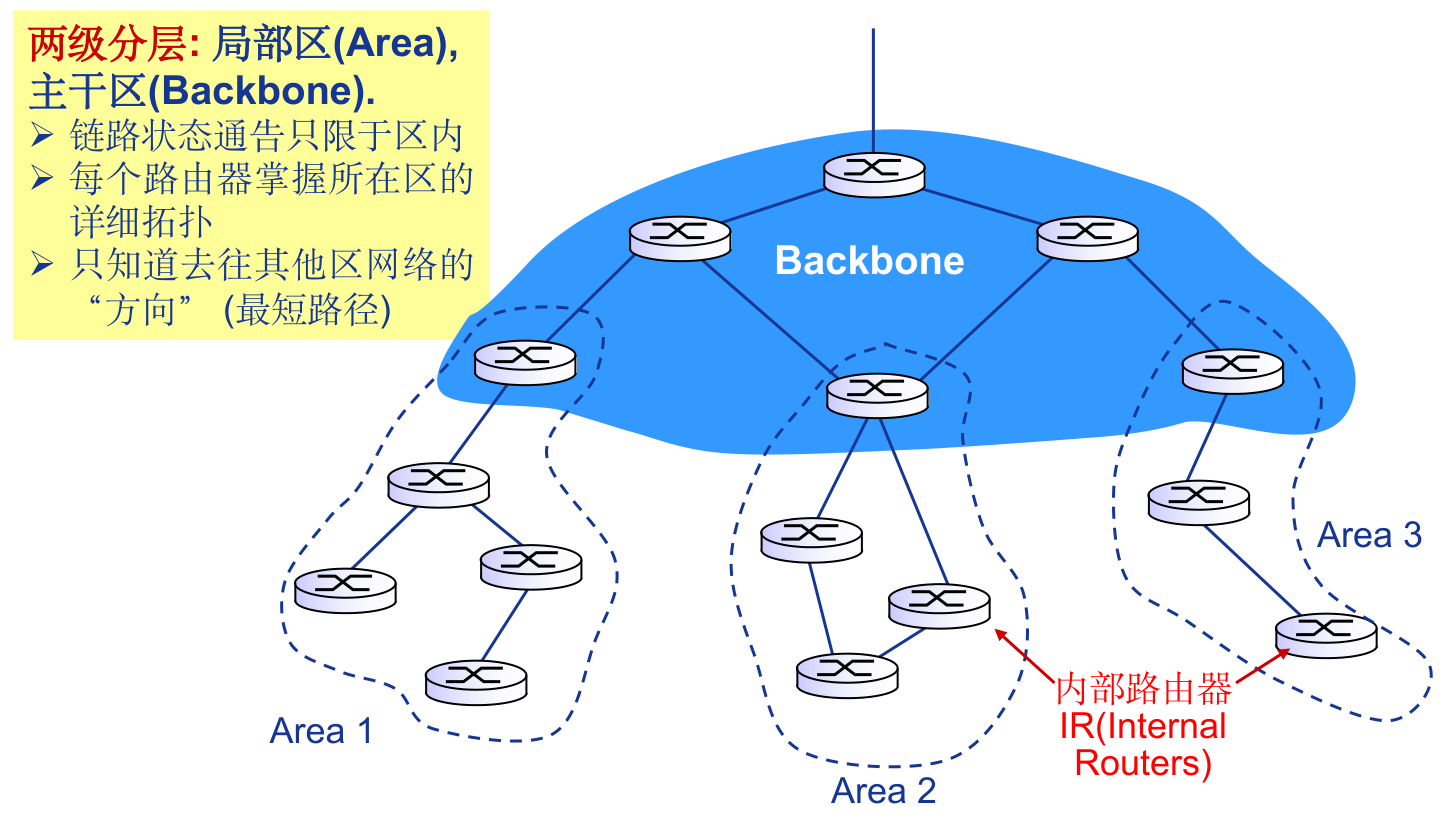
\includegraphics[width=.8\textwidth]{ch04-ospf-area.png}\caption{OSPF分区结构：区域经主干互连。来源：Chapter4-网络层.pdf，PDF第188页（显示页188），局部截取。}\end{figure}

\subsection{BGP：自治系统之间的策略路由}
\textbf{BGP}（边界网关协议）用于AS间交换目的前缀可达性；两个对等体通过TCP会话交换路径信息。eBGP在不同AS对等体间交换，iBGP在同一AS内部传播。路径通告包括\textbf{AS-PATH}（所经过的AS序列，可用于检测包含自身AS的环路）和\textbf{NEXT-HOP}（下一跳属性）。接收方可依据策略接受或拒绝，进而依据本地偏好、AS路径长度、到下一跳的内部代价等选择。策略优先于单纯的最短距离，不是每条学到的路由都会被再次通告。

BGP会话先建立TCP连接，再用OPEN协商参数；UPDATE通告或撤销路径，KEEPALIVE维持会话，NOTIFICATION报告差错并关闭会话。课件中的商业关系例表明：某AS未必愿意为两个非客户之间免费中转，故出口策略会限制可通告的路径。RIP、OSPF解决AS内部路由，BGP主要解决AS间可达性和策略。
\par\small\noindent 来源：课件 PDF 第180--200页；教材 PDF 第199--206页（印刷第188--195页）。\normalsize

\annotationarea[4]
\section{课件例题与综合练习详解}
\subsection{课件例2：链路状态算法Dijkstra的第二个算例}
从 $u$ 出发，课件 PDF 第156--157页给出另一组链路费用。按表格逐轮从未确定结点中选当前费用最小者，确定次序为 $u,x,y,v,w,z$；最终费用为 $D(v)=2$、$D(x)=1$、$D(y)=2$、$D(w)=3$、$D(z)=4$。例如 $u$ 到 $w$ 的路径是 $u\to x\to y\to w$，总费用 $1+1+1=3$；$u$ 到 $z$ 的路径是 $u\to x\to y\to z$，总费用 $1+1+2=4$。转发表记录第一跳：去往 $v$ 走 $(u,v)$，去往 $x,y,w,z$ 均先走 $(u,x)$。注意，费用表中的前驱结点与转发表中的下一跳不是同一概念：若前驱不是源结点，要沿前驱链回溯到源结点后的第一个结点。\annotationarea[4]

\subsection{课件例：距离向量的更新与链路失效}
课件 PDF 第163--164页的三结点例中，$x$ 到 $y$ 的链路费用为2，到 $z$ 的费用为7，$y$ 到 $z$ 的费用为1。$x$ 收到邻居通告后计算
\[
D_x(z)=\min\{c(x,y)+D_y(z),c(x,z)+D_z(z)\}=\min\{2+1,7+0\}=3,
\]
因此经 $y$ 到 $z$，而不是直连 $z$。\par
课件 PDF 第177--178页再给出R1--R2--R3线性拓扑。若到 $192.168.2.0/23$ 的已收敛跳数为 $(3,2,1)$，R3发现该网不可达后，R2尚保留旧消息，可能继续将R1的可达性误导到已断开的网络。第一轮交换后各路由器距离为 $(3,4,3)$；第二轮后为 $(5,4,5)$。因此题目问第二轮后R1的距离向量，答案是5跳。这个数字尚未表示网络已正确收敛，而是显示坏消息可能逐步增加度量。\annotationarea[4]

\subsection{课件例2：NAT端口映射}
课件 PDF 第135--138页的校园网中，R2后面的Web服务器是 $192.168.1.2$，外侧地址为 $203.10.2.2$；R3后面的H2地址也为 $192.168.1.2$，R3外侧地址为 $203.10.2.6$。两处相同的私有地址属于不同局域网。要让H2、H3访问Web默认端口，R2需静态映射
\[
203.10.2.2:80\longleftrightarrow 192.168.1.2:80.
\]
R3还须为内部主机配置出站NAT，使用R3的公网地址及端口区分会话。H2发出的HTTP数据报源IP为 $192.168.1.2$、目的IP为 $203.10.2.2$；R3做源地址转换后变为 $203.10.2.6\to203.10.2.2$；R2做目的地址转换后变为 $203.10.2.6\to192.168.1.2$。回包按相反次序查表改写。\annotationarea[4]

\subsection{课件例：从 /24 中分配三个局域网}
课件 PDF 第201--202页要求从地址块 $192.168.1.0/24$ 中划分三个局域网。已有子网 $192.168.1.0/25$ 已占用，剩余地址块为 $192.168.1.128/25$。三个局域网分别至少需要60、30、30个可用地址。\par
先给60台主机的网络分配/26：块大小64、可用62个；两个30台网络各分配/27：块大小32、可用30个。分配结果为：
\begin{center}\begin{tabular}{lllll}\toprule 局域网 & 网络/前缀 & 掩码 & 广播地址 & 可用地址范围\\\midrule
1 & $192.168.1.128/26$ & $255.255.255.192$ & $192.168.1.191$ & $192.168.1.129$--$192.168.1.190$\\
2 & $192.168.1.192/27$ & $255.255.255.224$ & $192.168.1.223$ & $192.168.1.193$--$192.168.1.222$\\
3 & $192.168.1.224/27$ & $255.255.255.224$ & $192.168.1.255$ & $192.168.1.225$--$192.168.1.254$\\\bottomrule\end{tabular}\end{center}
分配时先满足最大需求，并保证每个网络地址按块大小对齐；网络地址和广播地址不计入普通可用主机数。\annotationarea[4]

\subsection{课件例：为R1填写路由表并在R2聚合}
课件 PDF 第203--206页中，R1的E1、E2、E3、E4分别直连前三个新子网及已分配的 $192.168.1.0/25$；R1经L0到R2，下一跳地址为 $192.168.2.2$。相关路由项如下：
\begin{center}\begin{tabular}{llll}\toprule 目的网络 & 掩码 & 下一跳 & 接口\\\midrule
$192.168.1.128$ & $255.255.255.192$ & 直连 & E1\\
$192.168.1.192$ & $255.255.255.224$ & 直连 & E2\\
$192.168.1.224$ & $255.255.255.224$ & 直连 & E3\\
$192.168.1.0$ & $255.255.255.128$ & 直连 & E4\\
$201.18.3.0$ & $255.255.255.128$ & $192.168.2.2$ & L0\\
$201.18.3.254$ & $255.255.255.255$ & $192.168.2.2$ & L0\\
$0.0.0.0$ & $0.0.0.0$ & $192.168.2.2$ & L0\\\bottomrule\end{tabular}\end{center}
R2到达上述四个 $192.168.1.x$ 子网都经R1的 $192.168.2.1$、接口L0，因此可用 $192.168.1.0/24$ 聚合。能聚合的条件是地址前缀连续、下一跳和输出接口相同，而且汇总后不把本来不可达的地址错误地指向该下一跳；若误导流量就会形成路由黑洞。更具体路由可依最长前缀匹配覆盖汇总路由。\annotationarea[4]

\subsection{课件例：主机配置与错误掩码}
课件 PDF 第207--209页的例子中，H1位于 $201.18.3.0/25$。示例配置为IP地址 $201.18.3.1$、掩码 $255.255.255.128$；默认网关为 $201.18.3.126$，DNS服务器为 $201.18.3.254$。H1和DNS不在同一子网，因此主机把DNS查询交给默认网关。\par
H2的地址是 $201.18.3.2$。若它误用 $255.255.255.0$，就会把 $201.18.3.254$ 判断为本地链路上的主机，直接广播ARP询问服务器的MAC地址。H2所在的实际链路是 $201.18.3.0/25$，DNS服务器在另一子网，ARP广播不会通过路由器，因此解析失败，DNS查询也发不出去。正确的/25掩码使H2判断DNS服务器在异网，继而用ARP寻找默认网关MAC，再把DNS数据报交给路由器转发。\annotationarea[4]

\subsection{课件例：BGP出口选择}
课件 PDF 第173--199页说明，若同一前缀可由多个自治系统到达，路由器先依据本地偏好和策略决定接受哪些路径；之后可按AS-PATH长度、到NEXT-HOP的自治系统内费用等准则选择。热土豆路由是在可用外部路径中选择AS内部代价较低的网关，不保证端到端路径最短。提供商AS通常只向其他网络通告符合其商业策略的路径，例如不替两个非客户AS免费转发彼此的流量。\annotationarea[4]

\section*{本章自查：先自己回答，再对照解析}
\begin{enumerate}[nosep]
\item A到B跨越路由器时，B的IP地址是否每跳改变？帧目的MAC是否每跳都相同？
\item \texttt{192.168.1.130/26} 的网络地址、广播地址分别是什么？
\item IPv4数据报总长4000字节、首部20字节、MTU为1500字节时，第二片偏移是多少？
\item RIP与OSPF各与哪一种基本路由算法对应？BGP又主要用于什么范围？
\end{enumerate}
\textbf{参考答案：}1. 普通转发中目的IP不变；每段链路重新封装，目的MAC对应本跳接收接口，可改变。2. /26每块64个地址，130落在128--191，网络地址为 \texttt{192.168.1.128}，广播为 \texttt{192.168.1.191}。3. 第一片载荷1480字节，因此第二片偏移为 $1480/8=185$。4. RIP对应距离向量，OSPF对应链路状态；BGP主要用于自治系统之间的路由与策略。
\annotationarea[2]


\chapter{传输层}

\noindent\textbf{本章要解决的问题。} 网络层把IP数据报送到目标主机；传输层还要把收到的数据交给主机中的正确应用进程，并按应用需要提供服务。本章按课件顺序学习：进程之间的逻辑通信、端口与套接字、UDP、可靠数据传输、TCP连接与字节流，以及TCP的流量控制和拥塞控制。

\section{传输层服务}
\textbf{进程}是正在运行的程序及其状态。网页浏览器、邮件程序和视频应用可以同时运行在同一台主机上。网络层主要识别\textbf{主机}，传输层再依据端口等信息把数据交给主机中的\textbf{进程}。因此，传输层提供的是端系统之间进程到进程的逻辑通信。

发送端的封装顺序是：应用数据加上传输层首部，形成TCP报文段或UDP数据报；再装入IP数据报，最后封装成链路层帧。接收端按相反方向逐层去掉首部并交付。传输层首部中的端口帮助分用；IP首部中的协议号帮助网络层区分TCP、UDP等上层协议。

传输控制协议TCP（Transmission Control Protocol）和用户数据报协议UDP（User Datagram Protocol）提供不同服务。TCP面向连接，提供可靠、按序的字节流，并带有接收端流量控制与网络拥塞控制；UDP无连接、首部短，不保证交付、按序或不重复。应用可以根据需要在UDP之上自己实现确认和重传。传输层协议运行在端系统上，路由器通常只处理IP层及以下的转发。

\annotationarea[4]
\small 来源：课件 \texttt{Chapter5-传输层.pdf}，PDF阅读器第3--8页；PDF第3页显示页为3，PDF第4--8页无独立显示页码。参考书PDF第235--236页（印刷第224--225页）。\normalsize

\section{多路复用与分用}
\textbf{多路复用}发生在发送端：多个应用进程把数据交给传输层，传输层分别加上端口等首部，再把报文交给网络层。\textbf{分用}发生在接收端：传输层检查收到报文段的首部，并将数据交给相应套接字。

\textbf{端口号}是传输层用于识别通信端点的16位数字。\textbf{套接字}是应用进程与传输层交互的端点；它会和本地地址、端口及协议等信息关联。端口数值在TCP与UDP中可以分别使用。

\begin{itemize}[nosep]
\item \textbf{UDP分用：}课件模型以目的IP地址和目的端口找到接收套接字；同一个UDP服务器端口可以接收来自多个客户端的数据报。应用仍能从每个数据报中读到源IP与源端口，以便回复。
\item \textbf{TCP分用：}已建立的连接通常由源IP、源端口、目的IP、目的端口四元组区分。多个客户端可以同时连接同一服务器IP和服务端口，因为每个连接的客户端端点不同。监听套接字负责接收新连接，建立后的连接由各自的连接套接字处理。
\end{itemize}

\begin{center}\begin{tabular}{lll}\toprule 传输协议 & 课件中的主要分用信息 & 同一服务端口能否接收多客户端\\\midrule
UDP & 目的IP地址、目的端口 & 可以，同一UDP套接字可收到多个源的数据报\\
TCP & 源/目的IP地址、源/目的端口四元组 & 可以，每条连接有独立四元组\\\bottomrule\end{tabular}\end{center}
\annotationarea[4]
\small 来源：课件PDF阅读器第9--17页；PDF第9、15、17页分别显示页9、15、17，PDF第10--12页无独立显示页码。参考书PDF第236--238页（印刷第225--227页）。\normalsize

\section{UDP用户数据报协议}
\subsection{UDP提供什么服务}
UDP（用户数据报协议）无须在发送数据前建立连接。发送方每次独立发送一个数据报，接收方可能收不到、收到乱序数据，或收到重复数据；UDP本身不自动重传，也不保证数据交付给应用。DNS查询、SNMP和部分实时音视频会使用UDP。应用如果需要可靠性，可在应用层增加确认、重传或特定错误恢复。

UDP首部固定8字节，由源端口、目的端口、长度、校验和四个各2字节的字段组成。长度以字节计，包含UDP首部与数据，不含IP首部。例如应用数据100字节，则UDP长度字段为108字节。

\subsection{UDP校验和的计算}
校验和用于发现传输中可能发生的位错误，不负责修复错误。IPv4的计算范围包含伪首部、UDP首部和应用数据。\textbf{伪首部}临时取自IP层的源/目的地址、协议号17和UDP长度，参与计算但不作为独立字段发送。若数据字节数为奇数，只在计算时末尾补一个0字节。

计算步骤：把校验和字段先置0；将待检内容按16位分组；用反码加法相加，把最高位的进位回卷到最低位；将最终和逐位取反，作为校验和。接收方按相同方式把校验和也纳入求和，结果全1表示未检测到错误，不代表绝对没有错误。

\textbf{课件手算例（PDF第23页）。} 课件给出两个16位字：
\[
1110011001100110\quad(\texttt{0xE666}),\qquad
1101010101010101\quad(\texttt{0xD555}).
\]
分步计算：
\[
\begin{aligned}
\texttt{0xE666}+\texttt{0xD555}&=\texttt{0x1BBBB},\\
\text{回卷最高位进位：}\quad\texttt{0xBBBB}+1&=\texttt{0xBBBC},\\
\text{逐位取反：}\quad\texttt{0xBBBC}&\longrightarrow\texttt{0x4443}
 = \texttt{0100010001000011}.
\end{aligned}
\]
因此校验和值为$\texttt{0x4443}$。若数据字更多，就继续逐个相加并回卷每次产生的进位。\annotationarea[4]
\small 来源：课件PDF阅读器第18--23页；PDF第19页显示页3，PDF第20--23页显示页与PDF页相同。参考书PDF第240--242、245页（印刷第229--231、234页）。\normalsize

\section{可靠数据传输}
\subsection{可靠交付需要哪些机制}
可靠交付的目标是：数据不错、不丢、不乱、不多。底层信道可能损坏、丢失或延迟分组，协议因此需要校验和、确认、序号、重传和定时器。课件用有限状态机描述发送方、接收方在不同事件后的动作；状态表示当前协议进展，事件可能是收到分组、收到确认、校验失败或定时器超时。

\begin{itemize}[nosep]
\item \textbf{rdt 1.0：}假设底层信道完全可靠，发送方发出、接收方交付即可。
\item \textbf{rdt 2.0：}考虑分组位错误；用校验和检错，接收方以ACK（acknowledgment，确认）确认正确分组，以NAK（negative acknowledgment，否定确认）报告损坏，发送方收到NAK后重传。基于确认和重传的机制称自动重传请求（ARQ，Automatic Repeat reQuest）。
\item \textbf{rdt 2.1：}ACK或NAK也可能损坏。发送方给数据分组加0/1序号；接收方根据期望序号识别重复分组，避免把重传数据重复交给应用。
\item \textbf{rdt 2.2：}不单独发NAK；接收方重复确认最近正确收到的分组。发送方收到不匹配的重复ACK时重传当前分组。
\item \textbf{rdt 3.0：}数据分组或确认都可能丢失或延迟；发送方启动定时器，若超时仍没有有效确认就重传。序号让接收方识别延迟到达的旧分组。
\end{itemize}

\textbf{事件例：ACK丢失。} 发送方发送序号0并启动计时器；接收方校验正确后向应用交付一次，并返回ACK0；ACK0在途中丢失。发送方超时重发序号0，接收方发现自己当前期待序号1，于是丢弃重复数据、再次回ACK0；发送方收到确认后再发送序号1。若没有序号，接收方无法分辨重传分组和新的相同数据。

\textbf{事件例：分组丢失。} 发送方发序号1后启动定时器；分组未到达，接收方没有可确认的数据；定时器到期，发送方重新发送序号1；接收方收到并交付一次，再回ACK1。

\textbf{事件例：定时器过早触发。} 发送方发出分组1，分组已经到达接收方并被交付，但ACK1返回较慢。发送方在ACK回来前超时并重发1；接收方按序号认出这是重复分组，不再次交付，只重发ACK1。发送方收到一个有效ACK后继续发下一个新分组。过早超时会产生多余重传，但序号避免了重复交付。

\annotationarea[4]
\small 来源：课件PDF阅读器第24--44页（该组课件页脚编号通常与PDF页相同）；参考书PDF第72--78页（印刷第61--67页）。\normalsize

\subsection{停等协议与流水线}
\textbf{停等}表示每发送一个分组，发送方都要等确认回来，之后才能发下一个。设分组长度为 $L$ bit，链路速率为 $R$ bit/s，则发送一个分组的时间为 $t_{\rm seg}=L/R$。RTT（Round-Trip Time，往返时间）在此按数据最后一位发出到ACK第一位回来计；ACK发送时长为 $t_{\rm ACK}$。忽略处理、排队和错误，则信道利用率为
\[
U_{\rm stop}=\frac{t_{\rm seg}}{t_{\rm seg}+\mathrm{RTT}+t_{\rm ACK}}.
\]

\textbf{课件例（PDF第45--47页）：}链路速率1 Gb/s、单程传播时延15 ms、数据分组1 KB，忽略ACK发送时长。若1 KB按1000 B计，分组发送时间为 $8000/10^9=8\,\mu s$；往返传播时间约30 ms。因此
\[
U\approx\frac{8\,\mu s}{30\,ms+8\,\mu s}\approx0.0267\%.
\]
发送方约每30 ms才能发出一个1 KB分组，所以平均数据速率约为$8{,}000\text{ bit}/0.030\text{ s}=267\text{ kb/s}$，即约33 KB/s，远低于链路容量。限制在于协议等待时间，而非物理链路速率。

\textbf{流水线}允许发送方在收到确认之前连续发多个分组。发送窗口大小 $W_s$ 表示最多可有多少个分组处于未确认状态。在理想无损、等长分组、ACK可忽略且接收端能够持续接收时，近似利用率为
\[
U\approx\min\left(1,\frac{W_s t_{\rm seg}}{t_{\rm seg}+\mathrm{RTT}+t_{\rm ACK}}\right).
\]
窗口增大可提升利用率，但也需要更大的序号空间与缓存，并受到流量控制和拥塞控制限制。

\annotationarea[4]

\subsection{GBN：累积确认，超时后退回重传}
\textbf{后退N帧（GBN）}发送方最多有 $N$ 个未确认分组在途。ACK(n)表示截至序号$n$（包含$n$）的分组都已正确收到，这是\textbf{累积确认}。接收方只接收当前期待的序号；若收到乱序分组，丢弃它并重复确认最近连续收到的序号。发送方通常为最早未确认分组维护一个定时器；超时后重发该分组及其后所有尚未确认的分组。

\textbf{课件例（PDF第59页）：}发送方已发序号0到7，收到ACK0、ACK2、ACK3。由于ACK3累计确认0到3，当前最早未确认分组是4。若此时定时器超时，重发4、5、6、7，共4帧。注意GBN的ACK(n)含义是“到n为止都收到”，TCP中的ACK号含义不同，见后文。

若序号字段为$k$位，序号空间大小是$2^k$；GBN的接收窗口为1，发送窗口最大为$2^k-1$，留出一个序号以避免新旧分组混淆。

\annotationarea[4]

\subsection{SR：逐个确认，重传缺失分组}
\textbf{选择重传（SR）}接收方分别确认每个分组，可缓存窗口内的乱序分组；发送方为未确认分组分别设定时器，超时只重发对应分组。接收方仍按序向上交付：当缺失的分组到达后，它可以把该分组及缓存中紧跟其后的连续分组依次交付。

\textbf{课件事件例（PDF第64页）：}发送窗口大小4，先发送0、1、2、3，其中2丢失。接收方交付0和1，分别回ACK0、ACK1；收到3时先缓存并回ACK3。发送方收到ACK0后发4，收到ACK1后发5；4和5到达后，接收方继续缓存并分别回ACK4、ACK5。随后2的计时器超时，发送方只重发2；接收方收到2后按序交付2、3、4、5，并滑动接收窗口。这个例子显示SR避免像GBN那样重复发送已经到达的3、4、5。

\begin{figure}[H]\centering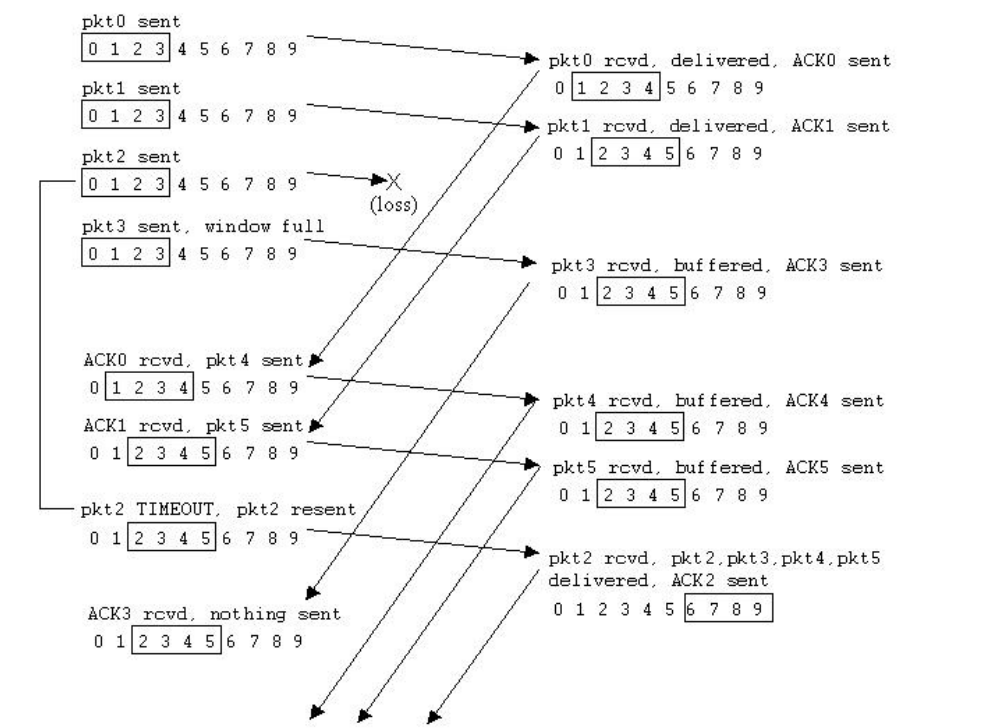
\includegraphics[width=.94\textwidth]{ch05-sr-example.png}\caption{选择重传的事件序列：2号分组丢失，接收方缓存3、4、5，发送方超时后只重传2。来源：Chapter5-传输层.pdf，PDF第64页（显示页64），局部截取。}\end{figure}

\textbf{序号空间限制。} 如果序号空间有$M=2^k$个值，发送窗口为$W_s$、接收窗口为$W_r$，为避免窗口回绕后把旧分组认成新分组，常见条件是$W_s+W_r\le M$。典型等大小SR窗口满足$W_s=W_r=W$，因此$W\le M/2=2^{k-1}$；停等的窗口均为1，至少需要1位序号。

\textbf{课件困境例（PDF第65--66页）：}序号为0、1、2、3，窗口大小3。发送端发送旧的序号0后，若它延迟很久；接收端先收到1、2并滑动窗口，再进入下一轮窗口0、1、2。此时旧序号0和新一轮序号0对接收端看起来相同，接收端可能把旧数据误当新数据交付。窗口3超过序号空间一半（2），无法仅凭序号消歧，因此SR窗口需满足上面的限制。

\annotationarea[4]
\small 来源：课件PDF阅读器第49--67页；参考书PDF第72--78页（印刷第61--67页）。\normalsize

\section{TCP：连接、字节流与首部}
\subsection{TCP提供面向连接的字节流}
TCP在两端建立连接状态后传送数据，提供全双工通信：两个方向可同时传数据，每个方向有各自的序号。\textbf{字节流}表示TCP把应用写入的数据看成连续字节，不保留每次写入的消息边界。一次写入100 B，对端可能分几次读取，也可能与后续写入一起读；应用若需要消息边界，必须自行定义长度或分隔符。

发送和接收两端都使用缓存。发送缓存保存尚未确认的数据以便重传；接收缓存暂存按序数据并等待应用读取。TCP的可靠性意味着协议会检测丢失、损坏和重复并尝试恢复；若连接长期不能恢复，应用仍可能收到错误。

\subsection{TCP首部和字节序号}
TCP首部固定部分为20 B；选项和填充可使首部最长达到60 B。数据偏移字段以4 B为单位表示首部长度，例如值5表示20 B。\textbf{MSS}是一个TCP段可携带的最大数据字节数，不包括TCP/IP首部。

\begin{figure}[H]\centering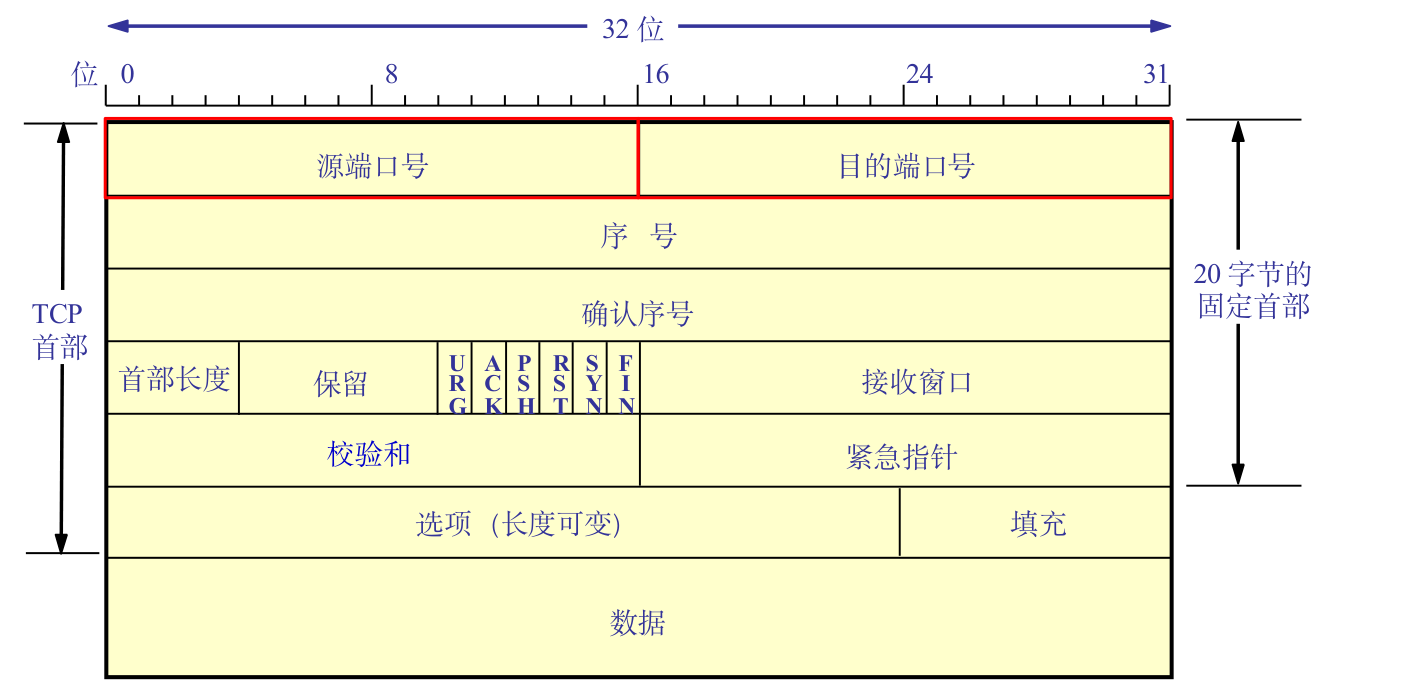
\includegraphics[width=.88\textwidth]{ch05-tcp-header.png}\caption{TCP基本首部字段布局，每行32 bit。来源：\texttt{Chapter5-传输层.pdf}，PDF第70页（显示页70），局部截取。}\end{figure}

\begin{center}\small\setlength{\tabcolsep}{4pt}
\begin{tabularx}{\textwidth}{>{\raggedright\arraybackslash}p{2.8cm}>{\centering\arraybackslash}p{1.2cm}>{\raggedright\arraybackslash}X}
\toprule 字段 & 位数 & 作用\\\midrule
源端口、目的端口 & 各16 & 标明两端应用进程的传输层端点\\
序号、确认号 & 各32 & 标明本段首字节编号，以及下一步期待收到的字节编号\\
数据偏移、保留、控制位 & 4、6、6 & 表示首部长度；保留位供协议扩展；经典控制位含URG、ACK、PSH、RST、SYN、FIN\\
接收窗口 & 16 & 通告接收方当前可接收的字节范围\\
校验和、紧急指针 & 各16 & 检错；URG有效时紧急指针标记紧急数据末端\\
选项与填充 & 可变 & 可携带MSS、时间戳、SACK等；填充使首部长度对齐到4 B\\\bottomrule
\end{tabularx}\end{center}

源端口和目的端口各16位；序号seq标明本段第一个数据字节的编号；确认号ack在ACK标志置位时有效，表示接收方\textbf{下一步期待的字节编号}。若接收方已连续收到截至400的字节，ack为401。接收窗口rwnd以字节通告接收端当前可用空间。校验和保护伪首部、TCP首部和数据；SYN用于同步连接两端的序号，FIN表示本方向发送结束，RST复位连接。PSH、URG及选项等字段按具体需要使用。TCP序号按$2^{32}$模回绕；SYN和FIN各占一个序号，纯ACK不消耗数据序号。

\textbf{课件序号例：}A发送seq=301、载荷100 B，则字节301--400被发送。若此前字节均连续收到，B回复ack=401。若A发送seq=401--500的数据段丢失，而后面的501--600到达，B仍回复ack=401，因为它期待的下一个连续字节仍是401。收到缺口后面的数据不等于确认了缺失字节。

课件PDF第80页另用单字节演示双向编号：A发seq=42的1 B，B确认ack=43；B用自己的序号空间发seq=79的1 B，A确认ack=80。两端各自维护发送序号，因此A的seq与B的seq不要求相等。

\textbf{GBN与TCP确认号的区别：}GBN的ACK(n)确认序号为$n$的分组以及此前分组；TCP的ack=$n$表示$n$之前的连续字节已收到、下一步期待字节$n$。两者都具有累计确认效果，但编号单位和字段含义不同。

\annotationarea[4]
\small 来源：课件PDF阅读器第68--80页；参考书PDF第247--249页（印刷第236--238页）。\normalsize

\section{TCP可靠传输与流量控制}
\subsection{确认、超时与快速重传}
TCP发送端缓存已发但尚未确认的数据，按累计确认推进最早未确认字节；接收端通常对连续收到的字节回复累计ACK。若ACK迟迟未到，发送端超时后重传最早未确认数据。

\textbf{快速重传}利用重复ACK及早发现缺口。例：接收方已收到字节0--999，下一段1000--1099丢失；之后三个更高序号的数据段到达，接收方仍发ack=1000。发送方收到三个重复ack=1000后，可立即重传从1000开始的数据段，不必等超时。重复ACK是丢失的线索，但也可能由乱序触发。

\textbf{RTT测量与重传超时。} SampleRTT是某数据段发出至其确认返回的测量值。段发生重传后，确认可能对应原发送或重传，来源不确定，通常不把这种样本用于估计。课件用指数加权平均计算：
\[
EstimatedRTT\leftarrow(1-\alpha)EstimatedRTT+\alpha SampleRTT,
\]
\[
DevRTT\leftarrow(1-\beta)DevRTT+\beta|SampleRTT-EstimatedRTT|,
\]
\[
TimeoutInterval=EstimatedRTT+4DevRTT.
\]
课件典型参数为$\alpha=0.125$、$\beta=0.25$。估计偏差越大，超时等待留出的余量越大。实际TCP还会使用计时器粒度、上下限和超时退避等细节。

\annotationarea[4]

\subsection{接收窗口与流量控制}
\textbf{流量控制}防止发送方把接收缓存填满，使接收应用有时间读取数据。接收方在TCP首部中通告rwnd；发送方在途未确认数据和新数据合计不能超过接收方允许的窗口。简化描述中，若接收缓存容量为$B$字节，缓存中尚未被应用读取的数据为$Q$字节，则$rwnd=B-Q$。

\textbf{例：}接收缓存容量4000 B，其中1000 B尚未被应用读取，则当前通告空间为3000 B。若发送窗口中已有1500 B未确认，接收端新空间为3000 B，则最多再发送1500 B，避免累计占用超过3000 B。若发送窗口为0，发送端暂停普通新数据；窗口更新可能丢失，TCP可用持续计时器和零窗口探测确认窗口是否重新开放。

\textbf{流量控制与拥塞控制的区别：}rwnd反映接收主机的可用缓存；cwnd反映发送端对网络可承受数据量的估计。简化模型允许未确认数据量不超过$\min(rwnd,cwnd)$；还需扣除已经在途的未确认数据，才得到当前可新发送的字节数。

\annotationarea[4]
\small 来源：课件PDF阅读器第81--92页；参考书PDF第252--254页（印刷第241--243页）。\normalsize

\section{TCP连接建立与释放}
\subsection{三次握手}
建立连接前，双方需要交换各自的初始序号并建立连接状态。设客户端初始序号为$x$、服务器为$y$：
\begin{enumerate}[nosep]
\item 客户端发SYN，seq=$x$。SYN占用一个序号，客户端进入SYN\_SENT。
\item 服务器回SYN+ACK，seq=$y$、ack=$x+1$，进入SYN\_RCVD。
\item 客户端回ACK，seq=$x+1$、ack=$y+1$。服务器收到后双方连接建立；第三段也可携带数据。
\end{enumerate}

\begin{figure}[H]\centering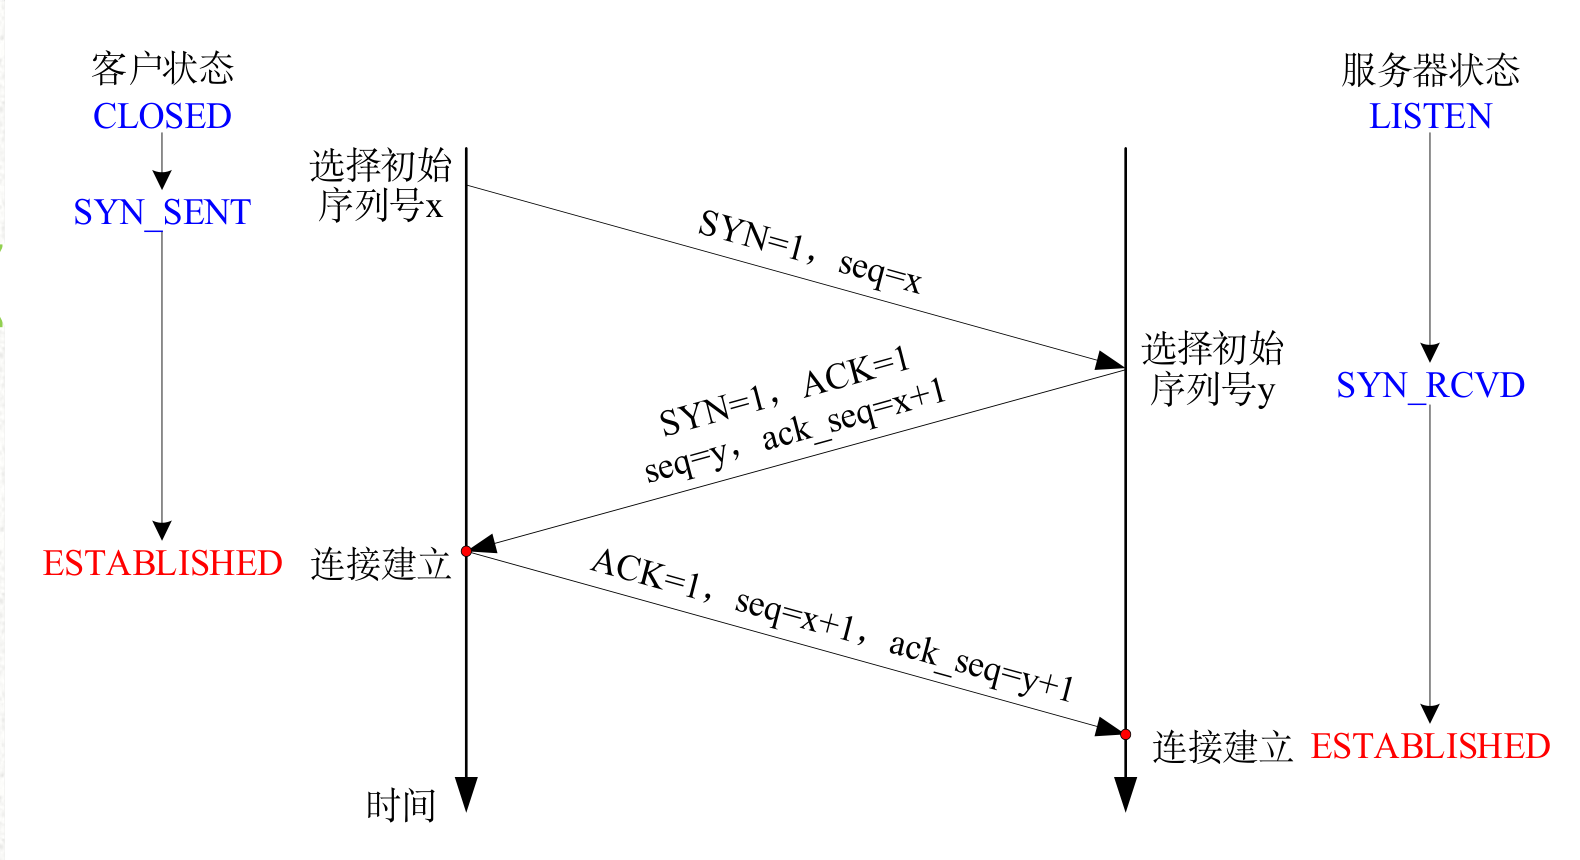
\includegraphics[width=.86\textwidth]{ch05-handshake.png}\caption{三次握手的报文顺序、序号确认和连接状态。来源：\texttt{Chapter5-传输层.pdf}，PDF第94页（显示页94），局部截取。}\end{figure}

图中两条竖线分别代表客户端和服务器，时间自上向下，斜箭头表示报文方向。第三次握手使服务器知道客户端收到了自己的初始序号，并帮助区分迟到的旧SYN和新连接。最终ACK到达之前服务器可能保留半连接状态，因此握手不能避免所有资源消耗。

\subsection{关闭连接与半关闭}
TCP是全双工的。一方发FIN只表示自己不再发送新数据，另一方向仍可能继续传数据，所以关闭常见为四个控制报文：
\begin{enumerate}[nosep]
\item 主动关闭方发FIN，进入FIN\_WAIT\_1；FIN占一个序号。
\item 被动方回ACK，进入CLOSE\_WAIT；主动方收到后进入FIN\_WAIT\_2。此时主动方还能接收对方数据，这种状态称半关闭。
\item 被动方完成发送后发FIN，进入LAST\_ACK。
\item 主动方回ACK并进入TIME\_WAIT；被动方收到后关闭。主动方等待$2MSL$后关闭，MSL表示报文段最大生存时间。
\end{enumerate}

\begin{figure}[H]\centering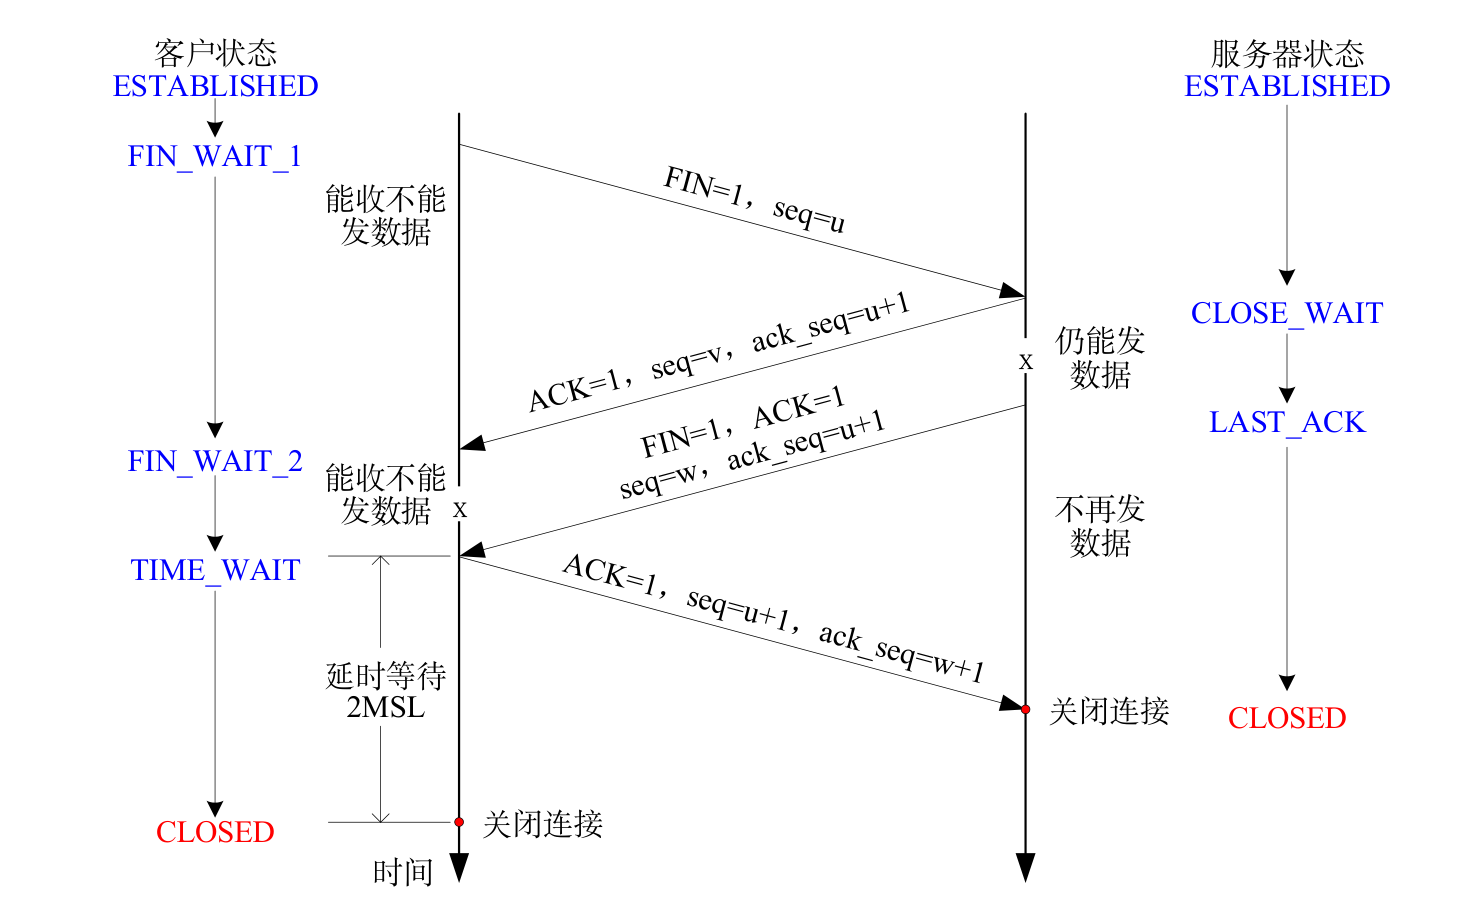
\includegraphics[width=.84\textwidth]{ch05-close.png}\caption{主动方与被动方关闭连接的报文及状态变化。来源：\texttt{Chapter5-传输层.pdf}，PDF第96页（显示页96），局部截取。}\end{figure}

ACK可与对方FIN合并，因此实际报文数并非必定正好四个。TIME\_WAIT等待可在最后ACK丢失时重新确认对方重传的FIN，并让旧报文从网络中消失。

\annotationarea[4]
\small 来源：课件PDF阅读器第93--97页；参考书PDF第249--251页（印刷第238--240页）。\normalsize

\section{TCP拥塞控制与性能}
\subsection{cwnd、慢启动与拥塞避免}
拥塞指网络中注入的流量超过某些链路或路由器的处理能力，排队时延会增长，缓存满时会丢包。TCP发送端看不到所有路由器内部状态，因此用丢包、超时、重复ACK或显式拥塞通知等信号调整发送速率。

\textbf{拥塞窗口cwnd}限制已发出但尚未确认的数据量，用来控制进入网络的流量。若发送方始终有数据、接收窗口足够且无其他瓶颈，粗略发送速率约为$cwnd/RTT$字节/秒。MSS是每段最大数据量，ssthresh是慢启动门限。

\begin{itemize}[nosep]
\item \textbf{慢启动：}课件教学模型初始cwnd为1 MSS；每收到一个新确认的满尺寸段，cwnd约增加1 MSS。因此在一个RTT内收到多个ACK时，cwnd约翻倍：1、2、4、8 MSS。课件例以MSS=500 B、RTT=200 ms起步，初始速率为$500\times8/0.2=20{,}000$ bit/s，即20 kb/s。慢启动的初始窗口小，但增长是指数式的。
\item \textbf{拥塞避免：}达到门限后，约每RTT增加1 MSS，即线性增长。课件用逐个ACK的小幅调整实现这一增长。
\item \textbf{丢包后的窗口调整：}三个重复ACK表示仍有数据在网络中传输，课件模型把ssthresh设为丢失时cwnd的一半，再执行快速重传并进入拥塞避免；超时被视为更严重拥塞，ssthresh设为原cwnd的一半、cwnd降至1 MSS，再进入慢启动。算法版本和教学模型的细节可能不同，做题时应按题目给定规则。
\end{itemize}

\begin{figure}[H]\centering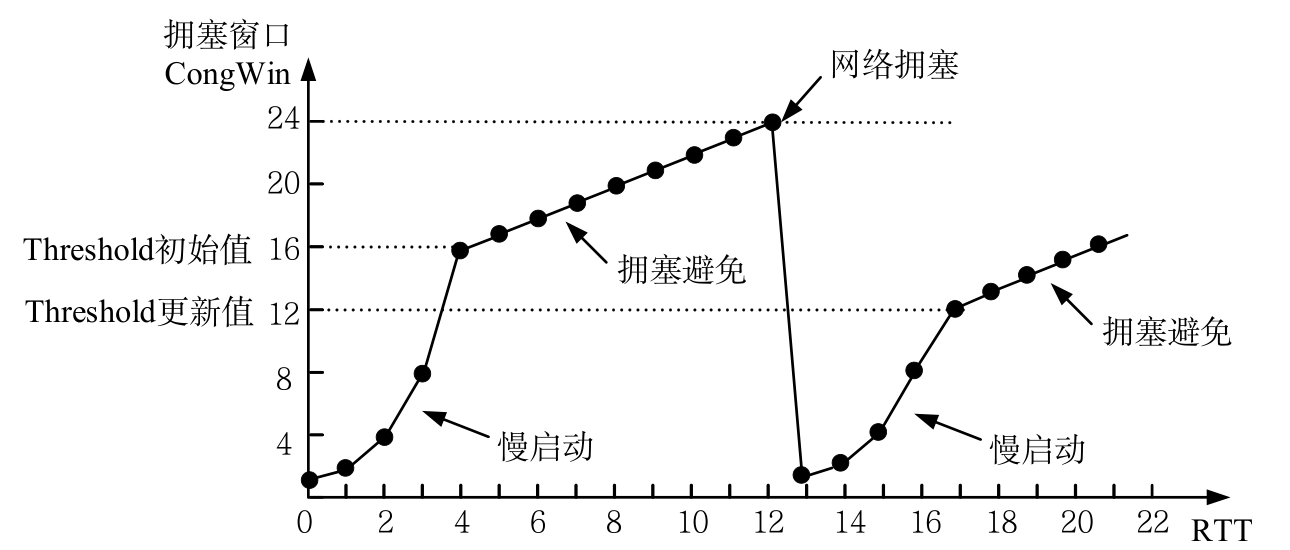
\includegraphics[width=.82\textwidth]{ch05-congestion.png}\caption{慢启动、拥塞避免及丢包后的窗口变化示意。来源：\texttt{Chapter5-传输层.pdf}，PDF第103页（显示页103），局部截取。}\end{figure}

\textbf{课件例题（PDF第108页）：}MSS=1 KB，cwnd=16 KB时发生超时。新门限为$16/2=8$ KB，cwnd回到1 KB。若之后各段都成功确认，慢启动每RTT约翻倍：第1个RTT后2 KB，第2个后4 KB，第3个后8 KB；达到门限后转为拥塞避免，第4个RTT结束时增加约1 KB至9 KB。

\subsection{快速恢复及其他拥塞信号}
TCP Reno教学模型收到三个重复ACK后，把门限设为原窗口的一半，并令cwnd暂时膨胀为$ssthresh+3MSS$；每多收到一个重复ACK，可再临时增加约1 MSS；收到确认新数据的ACK后，cwnd回到ssthresh并进入拥塞避免。窗口临时膨胀是因为重复ACK意味着有数据仍离开网络。发生超时则按更严重拥塞处理：cwnd回到1 MSS，重新慢启动。

课件还介绍：
\begin{itemize}[nosep]
\item \textbf{TCP CUBIC：}以曾发生丢包时的窗口$W_{max}$为参考，丢包后较快增长，接近$W_{max}$时放慢探测；窗口增长与距目标时刻$K$的时间差的立方相关。
\item \textbf{基于时延的拥塞控制：}以RTT增长作为队列可能变长的信号，目标是让瓶颈链路保持繁忙，同时避免缓存排队过多。最低观测RTT记为$RTT_{min}$，用$cwnd/RTT_{min}$估计无拥塞时的吞吐率，再与实测吞吐率比较，判断是否继续增加窗口。
\item \textbf{ECN显式拥塞通知：}支持ECN的路由器可在IP首部的ECN位标记拥塞；接收端在TCP确认中设置ECE等标志通知发送方，发送方据此降低发送速率。该机制需要网络和端系统共同支持。
\end{itemize}

\subsection{吞吐率、丢包率与公平性}
固定拥塞窗口为$W$个MSS、RTT稳定且发送方总有数据时，吞吐率近似为
\[
Throughput\approx\frac{W\times MSS\times8}{RTT}\quad\text{bit/s}.
\]
\textbf{课件例（PDF第110页）：}MSS=1500 B、RTT=100 ms，希望达到10 Gb/s，则
\[
W=\frac{10^{10}\times0.1}{1500\times8}\approx83{,}333\text{ 段}.
\]
该窗口代表需要同时在途的大量数据，尚未计入协议首部等开销。

课件PDF第109页给出的锯齿窗口近似为平均吞吐率$0.75W/RTT$：假设窗口在$W/2$与$W$之间线性增长，均值为$3W/4$，再除以RTT。课件该页把减半与“超时”相连，但第104--106页明确说超时将cwnd降至1 MSS；因此$0.75W/RTT$应理解为忽略慢启动、按稳定的加性增大/乘性减小锯齿周期得到的近似，不能把它当成每次超时之后的精确吞吐率。

\textbf{课件丢包率例（PDF第111页）：}窗口由$W/2$逐步增加至$W$时发送的段数近似为
\[
W/2+(W/2+1)+\cdots+W\approx3W^2/8+3W/4.
\]
当$W$较大时主项为$3W^2/8$，若该周期发生一个丢包，则丢包率近似$L\approx8/(3W^2)$。这是忽略低阶项的近似关系。

在理想公平模型中，$K$条特征相似、共享容量为$R$的TCP连接各自平均获得约$R/K$。实际结果受RTT、算法、路径和发送需求影响。课件例中已有9条连接：新应用只开1条TCP连接，约分得$R/10$；若开11条并行连接，课件近似写作$R/2$。按每条连接均分的简化假设，11条连接合计为$11R/20\approx0.55R$，与课件的$R/2$近似接近。这说明按连接公平不一定等于按应用公平。实际结果也会受实现和网络影响。若应用不做拥塞控制而用UDP持续高速发送，也可能挤占TCP流量。

\annotationarea[4]
\small 来源：课件PDF阅读器第98--123页；参考书PDF第254--256、277页（印刷第243--245、266页）。\normalsize

\section*{本章自查与解析}
先遮住答案作答，再用解析检查自己的推理。
\begin{enumerate}[nosep]
\item 一台Web服务器为何能用同一端口同时服务多个TCP客户端？
\item UDP数据长度为100 B，UDP长度字段应填多少？
\item TCP段seq=1000、数据长200 B，连续正确收到后确认号是多少？
\item GBN序号为0--7，已收到累积ACK3，之后定时器超时，要重传哪些未确认分组？
\item TCP的rwnd=5000 B、cwnd=3000 B，已有1000 B在途，简化模型下还能新发多少？
\item 主动方发FIN后为什么仍可能收到对方数据？
\end{enumerate}
\textbf{解析：}1. TCP连接按源/目的IP地址与端口四元组区分。2. UDP首部8 B，长度字段为108 B。3. 数据覆盖字节1000--1199，下一字节是1200，因此ack=1200。4. ACK3包含确认0--3，若窗口内4--7仍未确认，则重传4、5、6、7。5. 发送未确认数据上限为$\min(5000,3000)=3000$ B，扣除1000 B在途，可再发2000 B。6. FIN只关闭主动方发送方向；另一方向可继续发送到其自己发FIN为止。
\annotationarea[4]


\chapter{应用层}

\noindent\textbf{本章要解决的问题。} 网络应用由运行在端系统上的程序提供。为了让不同主机上的应用交换信息，需要规定应用程序如何寻址彼此、消息按什么格式组织、请求和响应何时发生，并选择能够满足应用需要的传输服务。本章沿课件顺序学习网络应用体系结构、进程通信、DNS、FTP、电子邮件、Web、P2P和Socket API。

\section{网络应用体系结构}
\subsection{客户机/服务器结构}
\textbf{网络应用}是运行在端系统上的程序，例如浏览器、邮件客户端和Web服务器。客户端与服务器是一次应用通信中的两个角色：\textbf{客户机（client）}发起请求并使用服务；\textbf{服务器（server）}等待请求、处理请求并返回结果。它们都是主机上运行的进程，不是专指某种硬件。

在\textbf{客户机/服务器结构（Client--Server，C/S）}中，服务器通常长期在线并有固定、可查找的地址；它可以用多台服务器提供服务和扩展处理能力。客户机间歇性接入网络，地址可能变化，并通过服务器取得服务；典型Web访问中，浏览器向Web服务器发送\textbf{超文本传输协议（HyperText Transfer Protocol，HTTP）}请求，服务器把页面对象作为响应发回。

这种结构容易集中管理，但服务能力受到服务器计算能力和网络带宽限制；服务器故障也可能使许多客户无法使用服务。课件以Web为例：PC上的浏览器和Mac上的浏览器分别向同一Web服务器发送HTTP请求，再接收HTTP响应。

\subsection{点对点结构与混合结构}
\textbf{点对点结构（Peer-to-peer，P2P）}中没有一直在线、负责全部服务的中央服务器。端系统称为\textbf{对等方（peer）}，可以彼此直接通信；节点既可能请求其他节点的资源，也可能向其他节点提供资源。节点可能间歇上线或更换IP地址。节点越多，能够提供的上传能力也可能越多，因此P2P可扩展性较好；但节点动态变化使管理、查找和维护更困难。

课件举出的\textbf{混合结构}是Napster：文件内容在节点之间用P2P传输，文件搜索与节点内容登记由中央服务器集中完成。可按下表区分三种结构。

\begin{center}\begin{tabularx}{.96\textwidth}{lXX}\toprule
结构 & 谁负责查找/协调 & 谁传输内容 \\\midrule
C/S & 服务器 & 客户端与服务器 \\
纯P2P & 节点之间协作，没有永久中央服务器 & 对等节点直接传输 \\
混合（课件Napster例） & 中央服务器登记内容并回答搜索 & 找到资源后由对等节点传输 \\\bottomrule\end{tabularx}\end{center}

P2P中的“对等”描述的是应用层的逻辑关系，不表示另建了一套物理互联网。实际网络仍由主机、路由器和链路组成；应用可以在其上建立自己的覆盖网络。\textbf{参考书补充：}P2P节点在下载时扮演客户角色，在向别人提供资源时又扮演服务器角色，因此“纯P2P”不等于系统中永远不存在请求方和提供方。

\annotationarea[4]
\small 来源：\texttt{Chapter6-应用层.pdf}，PDF阅读器第4--8页（显示页4--8）；参考书PDF第278--280页（印刷第267--269页）。\normalsize

\section{网络应用通信原理}
\subsection{进程、Socket与端口}
\textbf{进程}是主机上正在运行的程序。同一台主机上的进程可通过操作系统提供的进程间通信机制交换信息；不同主机上的进程则通过网络发送和接收消息。发起某次通信的一方在该次交互中是客户进程，等待请求的一方是服务器进程。即使在P2P应用中，也可以针对一次具体资源请求区分请求方和响应方。

应用进程通过\textbf{套接字（socket）}向传输层发送消息，并从传输层接收消息。可以把套接字想成进程的“门”：进程把消息交给门外的网络服务，网络服务把消息送到另一台主机相应的门口。应用程序通过套接字API选择传输协议并设置相关参数；实际的协议处理由操作系统和网络协议栈完成。

IP地址用于定位主机，但不足以定位主机中的某个进程，因为同一主机可能同时运行多个网络应用。\textbf{端口号（port number）}帮助传输层把数据交给正确的进程。课件给出的常见服务器端口例子是HTTP的80、邮件服务的25。应用端点通常用\textbf{IP地址+端口号}标识；TCP连接还需结合通信双方的地址和端口区分。端口是16位数值，服务器使用约定的服务端口等待请求，客户通常使用系统分配的临时端口发起通信。

\subsection{应用层协议规定什么}
\textbf{应用层协议}规定不同应用进程交换消息时必须遵守的约定，至少包括：
\begin{itemize}[nosep]
\item \textbf{消息类型：}例如请求消息和响应消息；
\item \textbf{语法/格式：}消息有哪些字段、字段如何排列和表示；
\item \textbf{语义：}每个字段中的信息代表什么；
\item \textbf{规则：}进程在什么情况下发送什么消息，以及如何响应。
\end{itemize}

由\textbf{RFC（Request for Comments，互联网标准与技术文档系列）}等公开标准定义的协议（例如HTTP）便于不同厂商的程序互操作；私有协议只由特定应用定义和使用，课件提到不少P2P文件共享应用采用私有协议。

\subsection{应用对传输服务的需求}
不同应用对网络服务的要求不同。网络电话可以容忍少量数据丢失，但对延迟敏感；文件传输要求数据可靠；视频应用需要足够的带宽；电子邮件等弹性应用则可以适应不同带宽。\textbf{弹性应用}指网络可用带宽变化时，应用仍可工作，只是传输速度或等待时间随之变化。

课件按应用列出传输需求。表中的“时间敏感”是对延迟的要求；“容忍丢失”表示少量数据丢失时应用仍可能继续工作，并不表示丢失没有影响。
\begin{center}\begin{tabularx}{.98\textwidth}{lXX}
\toprule 应用 & 数据丢失与带宽需求 & 时间敏感性 \\
\midrule
文件传输、电子邮件、Web文档 & 不容忍丢失；带宽弹性 & 否 \\
实时音频/视频 & 可容忍丢失；音频约5 kbit/s--1 Mbit/s，视频约10 kbit/s--5 Mbit/s & 是，约数百毫秒 \\
存储音频/视频 & 可容忍丢失；音频约5 kbit/s--1 Mbit/s，视频约10 kbit/s--5 Mbit/s & 是，通常可放宽到数秒 \\
交互式游戏 & 可容忍丢失；带宽需求为几kbit/s & 是，约数百毫秒 \\
即时消息 & 不容忍丢失；带宽弹性 & 视应用而定 \\
\bottomrule
\end{tabularx}\end{center}

课件所列Internet传输层服务如下。\textbf{传输控制协议（Transmission Control Protocol，TCP）}提供面向连接的可靠字节流；\textbf{用户数据报协议（User Datagram Protocol，UDP）}提供无连接的数据报服务。这里“提供可靠传输”表示协议负责发现未确认的数据并按协议机制重传；不表示传输时间有上限。

\begin{center}\begin{tabularx}{.96\textwidth}{lXX}\toprule
服务 & TCP & UDP \\\midrule
连接 & 面向连接，通信前建立连接 & 无连接，发送数据前不建立连接 \\
可靠性 & 可靠、按序交付字节流 & 不保证交付、按序或不重复 \\
流量控制 & 根据接收方能力限制发送速度 & 不提供 \\
拥塞控制 & 网络负载过重时限制发送速度 & 协议本身不提供 \\
延迟/带宽保证 & 不提供 & 不提供 \\\bottomrule\end{tabularx}\end{center}

应用选择TCP还是UDP，取决于是否需要连接、可靠交付、流量控制等服务。两者都不能单独承诺固定的端到端延迟或最小带宽。

课件还把常见应用与协议对应起来：
\begin{center}\begin{tabularx}{.96\textwidth}{l l l}
\toprule 应用 & 应用层协议例子 & 常用传输层协议 \\
\midrule
电子邮件 & SMTP & TCP \\
远程终端访问 & Telnet & TCP \\
Web & HTTP & TCP \\
文件传输 & FTP & TCP \\
流媒体 & 专有协议 & TCP或UDP \\
Internet电话 & 专有协议 & 通常UDP \\
\bottomrule
\end{tabularx}\end{center}

\annotationarea[4]
\small 来源：\texttt{Chapter6-应用层.pdf}，PDF阅读器第10--18页（显示页10--18）；参考书PDF第278--279页（印刷第267--268页）对应用模型作补充，第281页（印刷第270页）说明DNS使用UDP。\normalsize

\section{域名解析系统DNS}
\subsection{域名空间与域名服务器}
网络设备可用\textbf{互联网协议（Internet Protocol，IP）地址}识别，但数字地址不便于人记忆。\textbf{域名系统（Domain Name System，DNS）}提供域名与IP地址等信息之间的查询服务，也可提供主机别名、邮件服务器别名和Web服务器负载分配等信息。DNS是由多层命名服务器组成的分布式数据库，并配有查询协议；没有一台服务器保存全网所有域名记录。

域名按层次组织，从右向左由高层到低层。例如在\texttt{www.amazon.com}中，\texttt{com}是顶级域，\texttt{amazon}位于其下，\texttt{www}是更具体的主机名。常见顶级域包括\texttt{com}、\texttt{org}、\texttt{edu}以及国家代码域名（如\texttt{cn}）。域名中的各级名称由不同管理者维护，并可把一部分管理权委托给下级。

DNS查询会涉及以下几类服务器：
\begin{itemize}[nosep]
\item \textbf{本地域名服务器（local DNS server）：}主机默认向它发起查询。它通常由ISP、学校或组织提供；它不严格属于DNS层次中的一个级别，并可缓存先前获得的答案。
\item \textbf{根域名服务器（root DNS server）：}在本地服务器不知道下一步应问谁时，根服务器可指出相应顶级域服务器。课件称全球有13个根服务器；教材补充说明这是13个逻辑根服务器标识，每个可由多个冗余服务器组成。
\item \textbf{顶级域服务器（Top-Level Domain，TLD server）：}例如管理\texttt{com}域的服务器，能够指出下一步应查询的权威服务器。
\item \textbf{权威域名服务器（authoritative DNS server）：}负责某个组织所管理的域，保存该域中主机等资源记录的权威答案。
\end{itemize}

\textbf{递归查询}与\textbf{迭代查询}描述的是服务器收到查询后如何继续工作。递归查询要求被询问者替请求方完成后续查询，再返回最终答案；迭代查询则由服务器给出“下一步询问谁”的指引，原查询方继续联系后续服务器。常见组合是：主机对本地DNS服务器使用递归查询，本地DNS服务器对根、TLD和权威服务器逐级使用迭代查询。

\begin{figure}[H]\centering
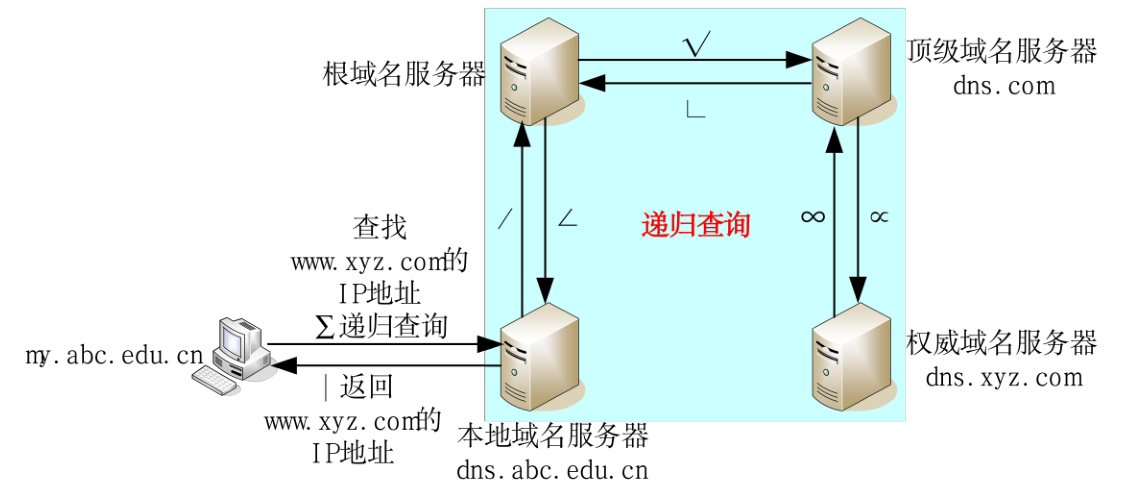
\includegraphics[width=.94\textwidth]{ch06-dns-recursive.png}
\caption{课件上半图：根服务器接手递归解析，并沿层级查询后把结果返回本地服务器，再答复主机。箭头表示查询或结果返回方向。来源：\texttt{Chapter6-应用层.pdf}，PDF第27页（显示页27），局部截取。}
\end{figure}
\begin{figure}[H]\centering
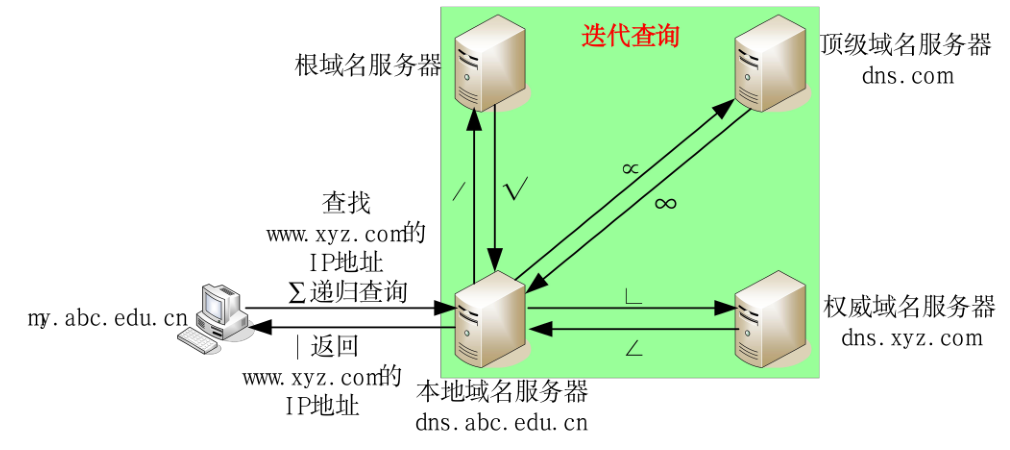
\includegraphics[width=.80\textwidth]{ch06-dns-iterative.png}
\caption{课件下半图：本地DNS服务器依次询问根、TLD和权威服务器；每次转介后，本地服务器自己向下一层查询。来源：\texttt{Chapter6-应用层.pdf}，PDF第27页（显示页27），局部截取。}
\end{figure}

\subsection{一次完整的域名解析}
以查询\texttt{www.amazon.com}为例，且假设主机和本地DNS服务器都没有可用缓存：
\begin{enumerate}[nosep]
\item 主机向本地DNS服务器发送查询请求；主机把后续查询委托给本地DNS服务器。
\item 本地DNS服务器先查自己的缓存。若未命中，它向根服务器发出迭代查询。
\item 根服务器返回\texttt{com}顶级域服务器的信息。本地DNS服务器据此向TLD服务器查询。
\item TLD服务器返回负责\texttt{amazon.com}的权威服务器信息；本地DNS服务器再向该权威服务器查询。
\item 权威服务器返回\texttt{www.amazon.com}对应的地址记录。本地DNS服务器缓存结果，并把答案交还主机。
\end{enumerate}

\textbf{课件例题（PDF第33页）。} 本地DNS服务器无缓存，使用递归方式解析另一个网络中的主机名，问主机与本地DNS服务器分别发几条查询消息？\textbf{解：}主机只向本地DNS服务器发起一次查询；本地DNS服务器作为代理发起后续递归解析。无缓存时主机和本地DNS服务器各自都发送一条查询，因此选A“一条、一条”。如果改成本地DNS服务器对外采用迭代方式，本地服务器会分别询问根、TLD和权威服务器，外部查询消息数就会多于一条；主机仍只需问本地服务器一次。

DNS记录会被服务器缓存一段时间，过期后删除。记录的\textbf{生存时间（Time To Live，TTL）}给出缓存有效期；缓存减少后续查询流量和等待时间，但也意味着记录更新后旧答案可能在TTL到期前继续被使用。

\subsection{资源记录与DNS消息}
DNS数据库中的一条记录称为\textbf{资源记录（Resource Record，RR）}，课件用\texttt{(name, value, type, ttl)}表示。常见类型如下：
\begin{center}\begin{tabularx}{.96\textwidth}{lXX}\toprule
类型 & Name & Value \\\midrule
A & 主机域名 & IPv4地址 \\
NS & 域名 & 该域权威域名服务器的主机名 \\
CNAME & 别名 & 对应的真实域名 \\
MX & 域名 & 为该域接收邮件的邮件服务器名 \\\bottomrule\end{tabularx}\end{center}

\textbf{注册域名的课件例。} 注册\texttt{networkutopia.com}时，注册机构把该域的NS记录以及权威服务器的A记录加入\texttt{com}的DNS信息；随后在权威服务器中为Web主机配置A记录，并为邮件服务器配置MX记录和对应的A记录。邮件地址中的主机部分由MX记录指向邮件服务器，不能把MX记录误认为邮件服务器IP地址。\textbf{课件记号提示：}第32页上方写\texttt{networkutopia.com}，后续示例中又出现\texttt{networkuptopia.com}（多出一个字母\texttt{p}）；本笔记沿用上方域名，只讲解记录配置关系，不据拼写差异推断两个域名的关系。

DNS查询与回复使用相同格式的消息。课件给出的固定首部长度为12字节，包含六组字段：16位消息标识、标志位、问题数、回答资源记录数、权威资源记录数和附加资源记录数。消息标识字段是16位编号，回复复制该编号，使请求方能匹配查询与回答。标志位说明这是查询还是回复、是否期望递归、服务器是否支持递归以及回答是否权威。首部之后依次是问题、回答、权威记录和附加信息四个部分；问题部分列出要查询的Name与Type，回答部分给出资源记录，权威部分可列出权威服务器信息，附加部分可放置帮助后续查询的信息。

\textbf{参考书补充：}DNS通常使用UDP承载查询，服务器端使用熟知端口53；若查询内容较大或响应需要可靠传输，也可能使用TCP。课件示例重点在命名层级和查询过程，没有展开这些传输层细节。

\annotationarea[4]
\small 来源：\texttt{Chapter6-应用层.pdf}，PDF阅读器第20--33页（显示页20--33）；参考书PDF第281--287页（印刷第270--276页）。课件第27页两幅查询图分别局部裁取；第33页递归查询选择题已逐步解答。\normalsize

\section{文件传输协议FTP}
\subsection{控制连接与数据连接}
\textbf{文件传输协议（File Transfer Protocol，FTP）}使用客户/服务器结构，在TCP上提供远程文件浏览、上传与下载。客户端先连接FTP服务器的TCP端口21，建立\textbf{控制连接}；用户名、密码、目录操作和传输命令经此连接发送。控制连接在整个FTP会话期间保持打开，文件内容不通过该连接传送。

服务器收到传输命令后，再为文件或目录列表建立\textbf{数据连接}。数据传输结束后数据连接关闭；若还要传另一个文件，可重新建立数据连接。控制命令与文件内容分开传输称为带外控制。课件图中的端口20是经典主动模式示例。

\begin{figure}[H]\centering
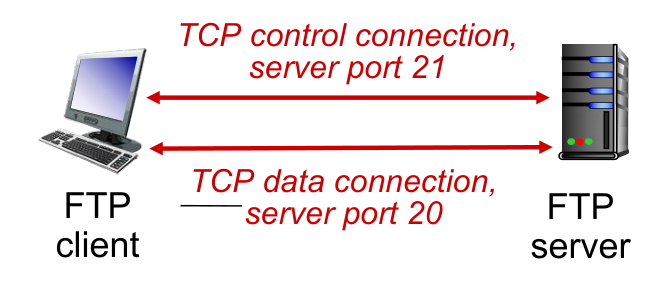
\includegraphics[width=.72\textwidth]{ch06-ftp-connections.png}
\caption{FTP将端口21上的控制连接与文件数据连接分开；课件图中数据连接的服务器端口20对应主动模式示意。来源：\texttt{Chapter6-应用层.pdf}，PDF第36页（显示页36），局部截取。}
\end{figure}

\textbf{参考书补充：}主动（PORT）模式下，服务器从自己的20号端口主动连到客户端提供的端口；被动（PASV）模式下，服务器告知客户端一个临时数据端口，由客户端主动连接。因此，端口20不是所有FTP数据连接都必然使用的端口。两种方式下控制连接都在服务器21号端口，客户端控制连接端口通常由系统分配。

\subsection{FTP命令与逐事件例子}
课件列出的控制命令以ASCII文本发送：\texttt{USER username}提交用户名，\texttt{PASS password}提交密码，\texttt{LIST}列出当前目录，\texttt{RETR filename}下载文件，\texttt{STOR filename}上传文件。服务器用状态码和文字回应，例如\texttt{331}表示用户名已收到、需要密码；\texttt{125}表示数据连接已打开、传输将开始；\texttt{425}表示无法打开数据连接；\texttt{452}表示写文件出错。

\textbf{下载事件例。}客户端连接服务器TCP 21号端口，随后通过控制连接发送登录信息；服务器验证成功后，客户端浏览目录并发送\texttt{RETR report.pdf}；服务器按当前传输模式建立数据连接；文件字节通过数据连接发送；文件传完后数据连接关闭，控制连接仍可继续用来下载另一个文件。\texttt{LIST}返回的目录列表也通过数据连接传输。

\annotationarea[4]
\small 来源：\texttt{Chapter6-应用层.pdf}，PDF阅读器第35--37页（显示页35--37）；参考书PDF第287--293页（印刷第276--282页）。主动/被动模式为参考书对课件双连接机制的补充。\normalsize

\section{电子邮件}
\subsection{系统组成与邮件投递}
电子邮件是一种异步通信方式：收件人不必与发件人同时在线。\textbf{用户代理（User Agent，UA）}是邮件客户端，用于撰写、发送、接收和管理邮件；\textbf{邮件服务器}负责接收邮件、暂存待发送邮件，并把来信放入收件人的邮箱。\textbf{简单邮件传输协议（Simple Mail Transfer Protocol，SMTP）}用于发送邮件及邮件服务器之间的投递；\textbf{邮局协议第3版（Post Office Protocol version 3，POP3）}、\textbf{互联网报文存取协议（Internet Message Access Protocol，IMAP）}或Web页面使用的HTTP可用于用户读取邮件。

\begin{figure}[H]\centering
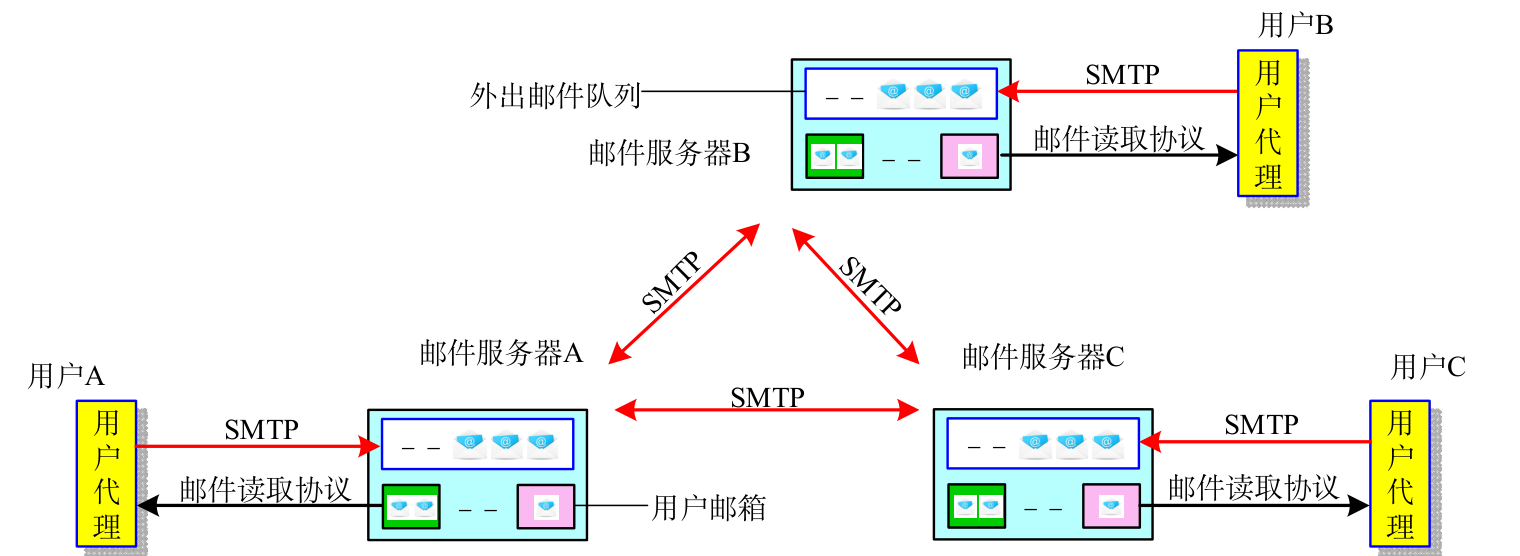
\includegraphics[width=.96\textwidth]{ch06-email-system.png}
\caption{邮件客户端把邮件交给邮件服务器；邮件服务器之间用SMTP投递，收件人通过邮件读取协议访问邮箱。箭头表示协议方向。来源：\texttt{Chapter6-应用层.pdf}，PDF第39页（显示页39），局部截取。}
\end{figure}

一次常见邮件流程为：发件人用用户代理撰写邮件并提交给发送端邮件服务器；邮件服务器把邮件放入外出队列；发送端服务器作为SMTP客户连接接收端邮件服务器并发送邮件；接收端服务器把邮件存入收件人邮箱；收件人之后通过POP3、IMAP或Web邮件读取。邮件服务器既能作为SMTP服务器接收邮件，也能作为SMTP客户向下一台邮件服务器发送邮件。

\subsection{SMTP及消息格式}
\textbf{简单邮件传输协议（Simple Mail Transfer Protocol，SMTP）}通过TCP可靠发送邮件，服务器端熟知端口为25。SMTP采用命令/响应方式，课件按握手、传输、关闭三个阶段说明。典型会话如下：

\begin{quote}\small\ttfamily
S: 220 hamburger.edu\\
C: HELO crepes.fr\\
S: 250 Hello crepes.fr, pleased to meet you\\
C: MAIL FROM: <alice@crepes.fr>\\
S: 250 Sender ok\\
C: RCPT TO: <bob@hamburger.edu>\\
S: 250 Recipient ok\\
C: DATA\\
S: 354 End mail with a line containing only a period\\
C: Do you like ketchup?\\
C: How about pickles?\\
C: .\\
S: 250 Message accepted for delivery\\
C: QUIT\\
S: 221 Closing connection
\end{quote}

读这段交互时，\texttt{C}是当前SMTP客户，\texttt{S}是服务器。\texttt{HELO}标识客户端；\texttt{MAIL FROM}给出发件人；\texttt{RCPT TO}指定收件人；\texttt{DATA}后开始传邮件内容；只含一个句点的行结束邮件内容；\texttt{QUIT}请求关闭会话。这里的客户端可以是用户代理，也可以是发送端邮件服务器。

SMTP连接通常在一次邮件传送会话中保持打开。课件所述基础SMTP邮件正文使用7位ASCII字符；HTTP与SMTP都使用可读文本命令和状态码，但方向和消息组织不同：HTTP通常由客户拉取对象，SMTP由发送方把邮件推送到接收方；HTTP的多个对象通常分别响应，邮件内容可由多个部分组成。

邮件内容有首部和主体，中间以空行分隔。常见首部行包括\texttt{From}、\texttt{To}和\texttt{Subject}；主体是邮件正文。课件的示例格式如下：
\begin{quote}\small\ttfamily
From: alice@crepes.fr\\
To: bob@hamburger.edu\\
Subject: Picture of yummy crepe.\\
\\
邮件正文……
\end{quote}

\textbf{MIME（Multipurpose Internet Mail Extensions，多用途互联网邮件扩展）}让邮件可以表示非ASCII文本和图像等多媒体内容。它通过邮件首部说明内容类型与编码方式，例如：
\begin{quote}\small\ttfamily
Content-Type: image/jpeg\\
Content-Transfer-Encoding: base64
\end{quote}
编码后的内容仍可经基础邮件传输方式传送。MIME扩展邮件格式和编码，不取代SMTP。课件第45页把MIME相关RFC写为“2045、2056”。其中RFC 2056的标题是“Uniform Resource Locators for Z39.50”，MIME Part Two对应RFC 2046；结合参考书在本节引用RFC 2045，可确认课件此处应为“2045、2046”，将“2056”订正为“2046”（\href{https://www.rfc-editor.org/info/rfc2046/}{RFC 2046}）。

\subsection{邮件读取：POP3与IMAP}
\textbf{邮局协议第3版（Post Office Protocol version 3，POP3）}用于用户代理从邮件服务器读取邮件。用户先用\texttt{USER}和\texttt{PASS}完成认证，服务器以\texttt{+OK}或\texttt{-ERR}回应；用户随后可用\texttt{LIST}列出邮件、\texttt{RETR}取回邮件、\texttt{DELE}标记删除，最后用\texttt{QUIT}结束会话。POP3可采用“下载并删除”或“下载并保留”的方式。按课件的基本模型，POP3不在服务器维护跨会话的文件夹状态。

\textbf{互联网报文存取协议（Internet Message Access Protocol，IMAP）}通常把邮件留在服务器上，支持用文件夹组织邮件，并保存跨会话的文件夹名、邮件与文件夹对应关系等状态。相较之下，POP3规则简单、功能较少。通过浏览器使用Web邮箱时，浏览器与邮件服务之间可用HTTP交互。

\textbf{POP3逐事件例。}用户代理发送\texttt{USER bob}，服务器以\texttt{+OK}回应；代理发送\texttt{PASS}，验证成功后用\texttt{LIST}获取邮件编号和大小；发送\texttt{RETR 1}读取1号邮件；若采用下载并删除方式，再发\texttt{DELE 1}；最后发\texttt{QUIT}关闭会话。若选下载并保留，读取后不删除服务器副本。

\annotationarea[4]
\small 来源：\texttt{Chapter6-应用层.pdf}，PDF阅读器第39--49页（显示页39--49）；参考书PDF第294--300页（印刷第283--289页）。课件第45页的RFC编号已按RFC 2046订正并附来源。\normalsize

\section{万维网与HTTP}
\subsection{Web对象、URL与HTTP交互}
\textbf{万维网（World Wide Web，WWW）}由相互链接的网页和网页对象构成。网页中的对象可以是\textbf{超文本标记语言（HyperText Markup Language，HTML）}文件、图片、视频或脚本等。\textbf{统一资源定位符（Uniform Resource Locator，URL）}标识资源的位置和访问方式，课件给出的一般形式为
\[
\texttt{scheme://host:port/path}.
\]
其中scheme表示访问资源的协议，host是服务器域名或IP地址，port是服务器端口，path指出主机上的资源位置；若端口省略，则使用协议约定的默认值。URL例子\url{www.someschool.edu/someDept/pic.gif}中，前半部分是主机名，后半部分是路径。

\textbf{超文本传输协议（HyperText Transfer Protocol，HTTP）}是浏览器和Web服务器交换请求、响应的应用层协议。课件基础模型中，浏览器先建立到服务器TCP 80端口的连接，再经连接发送HTTP请求并接收响应。HTTP协议本身是\textbf{无状态}的：服务器不因一次请求而自动记住同一客户以前请求过什么。底层TCP提供可靠字节流，但不意味着HTTP有固定响应时限。

\subsection{HTTP请求与响应消息}
HTTP消息采用文本形式。请求消息由请求行、若干首部行、空行和可选消息体组成。请求行包含方法、资源路径和协议版本；首部行传递主机名、连接方式、浏览器类型或语言偏好等信息。课件示例：
\begin{quote}\small\ttfamily
GET /somedir/page.html HTTP/1.1\\
Host: www.someschool.edu\\
User-agent: Mozilla/4.0\\
Connection: close\\
Accept-language: fr\\
\\
\end{quote}
首行表示获取资源；空行表示请求首部结束。响应消息由状态行、首部行、空行和可选消息体组成：
\begin{quote}\small\ttfamily
HTTP/1.1 200 OK\\
Connection: close\\
Date: Thu, 06 Aug 1998 12:00:15 GMT\\
Server: Apache/1.3.0 (Unix)\\
Last-Modified: Mon, 22 Jun 1998\\
Content-Length: 6821\\
Content-Type: text/html\\
\\
……请求的HTML对象……
\end{quote}

常用请求方法：\texttt{GET}取回对象；\texttt{POST}把用户表单等内容放在消息体中提交；\texttt{HEAD}请求首部而不取回对象主体；\texttt{PUT}把消息体中的对象存入指定URL；\texttt{DELETE}删除指定URL标识的对象。使用GET提交表单时，输入可编码到URL的查询部分，例如\texttt{/animalsearch?monkeys\&banana}；POST则把输入放在请求消息体中。

响应状态码在状态行中，课件示例包括：\texttt{200 OK}表示请求成功；\texttt{301 Moved Permanently}表示资源已永久移动；\texttt{400 Bad Request}表示请求有误；\texttt{404 Not Found}表示未找到资源；\texttt{505 HTTP Version Not Supported}表示服务器不支持所请求的HTTP版本。响应首部中的\texttt{Content-Length}表示主体长度，\texttt{Content-Type}说明主体类型。

\subsection{连接方式和HTTP响应时间}
\textbf{非持久连接}中，一个TCP连接传输一个对象；HTTP/1.0课件模型采用这种方式。若HTML页面引用图片，每个对象都需另建TCP连接。\textbf{持久连接}中，服务器发送完响应后保持TCP连接打开，后续请求和对象可复用该连接；HTTP/1.1课件模型默认采用持久连接。

\textbf{往返时间（Round-Trip Time，RTT）}是一个小分组从客户端到服务器并返回所经历的时间。为解释课件的时延公式，作如下假设：忽略DNS解析、排队、处理和小请求的发送时长，TCP按课件图的方式建立连接，服务器收到HTTP请求后开始返回对象。
\begin{itemize}[nosep]
\item 请求一个对象的非持久连接响应时间约为$2\mathrm{RTT}+t_{\mathrm{obj}}$：一个RTT用于建立TCP连接，另一个RTT用于发送请求并等到响应开始到达，$t_{\mathrm{obj}}$是对象传输时间。
\item 非流水持久连接只建立一次TCP连接，但客户必须等上一个对象响应后才请求下一个对象。若网页含基本HTML对象和$k$个引用对象，理想化总时间约为$\mathrm{RTT}+(k+1)\mathrm{RTT}+\sum t_i=(k+2)\mathrm{RTT}+\sum t_i$。
\item 流水持久连接允许客户尽快连续发出多个请求。在课件的理想模型中，基本HTML对象先需约$2\mathrm{RTT}$；解析HTML后，对引用对象的请求与响应可在约$1\mathrm{RTT}$内完成，再加对象传输时间。
\item 浏览器也可并行打开多个非持久TCP连接，使多个引用对象同时传输；并行能缩短对象组的等待时间，但增加连接和服务器资源开销。
\end{itemize}

\textbf{按课件公式计算的例子。} 若RTT为80 ms，对象大小为2 Mbit，瓶颈传输速率为10 Mbit/s，则对象传输时间为$2/10=0.2$ s。忽略其他延迟，单对象非持久连接响应时间约为$2\times0.08+0.2=0.36$ s。

\begin{figure}[H]\centering
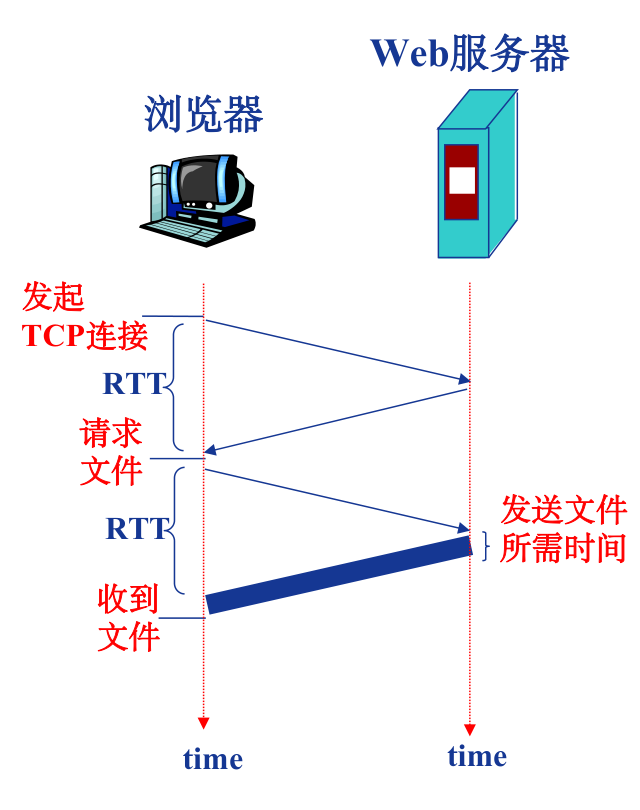
\includegraphics[width=.46\textwidth]{ch06-http-timing.png}
\caption{HTTP/1.0单对象时间线：第一段RTT建立TCP连接，第二段RTT发送请求并等响应开始到达，深色斜条表示对象传输时间。来源：\texttt{Chapter6-应用层.pdf}，PDF第63页（显示页63），局部截取。}
\end{figure}

\textbf{HTTP/1.1流水与队头阻塞。}非流水方式中，收到一个响应后才发下一个请求；流水方式中，发现引用对象后即可连续发送请求。HTTP/1.1按序在一个TCP字节流上传输数据。如果前面的大对象排在小对象之前，小对象会等待；若TCP遇到丢包恢复，后续字节也要等缺失数据补齐。这种等待称为\textbf{队头阻塞（Head-of-Line blocking，HOL blocking）}。

\textbf{HTTP/2与HTTP/3。}课件说明HTTP/2把对象拆成帧，让不同对象的帧交替传输，并可按客户指定的优先级安排对象；课件也提到服务器推送客户尚未请求的对象。交错帧减少对象排队造成的应用层阻塞，但若共享TCP连接丢包，TCP仍要按序交付数据，仍可能暂停多个对象。HTTP/3采用QUIC（Quick UDP Internet Connections）承载HTTP：QUIC运行在UDP之上，在应用层实现可靠性、拥塞控制、连接建立和加密相关功能，并让多个应用级流共享连接。课件强调，一个流的数据丢失不必阻塞其他流继续交付，因而可避免跨流的TCP队头阻塞。

课件第73页把QUIC建立连接标成“1轮握手”，并与单独进行TCP和TLS握手的“2轮”作对比。这是课件用于解释减少建立时延的示意；实际握手时延会依协议版本、连接状态和实现条件而变，计算题应按题目给定条件使用。

\subsection{代理缓存、条件GET与Cookie}
\textbf{Web缓存/代理服务器（Web cache/proxy）}保存近期访问的对象。浏览器把HTTP请求发给代理：若缓存命中，代理直接把对象返回，代理此时作为服务器；若未命中，代理作为客户向原始服务器请求对象，取得后返回浏览器并保存副本。缓存靠近用户时可减少访问时延，也能降低组织出口链路流量。

\begin{figure}[H]\centering
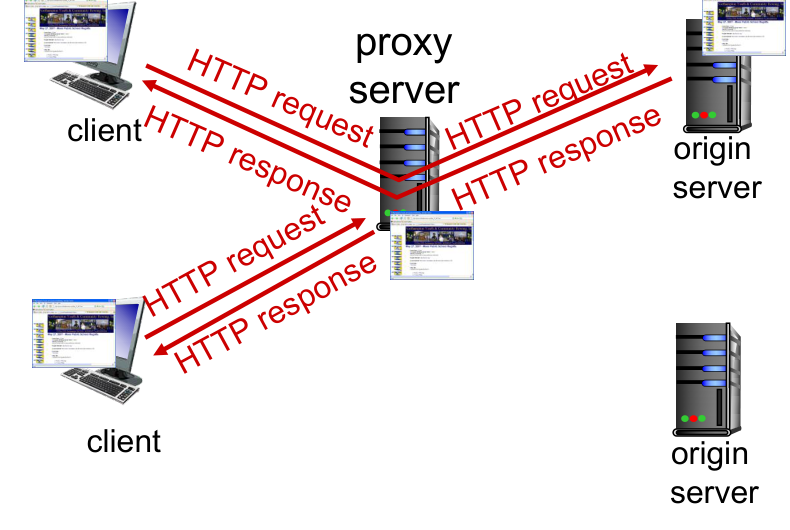
\includegraphics[width=.80\textwidth]{ch06-web-cache.png}
\caption{Web缓存同时面对客户端和原始服务器：命中时从代理直接返回，未命中时由代理请求源站并把对象缓存。箭头表示HTTP请求或响应方向。来源：\texttt{Chapter6-应用层.pdf}，PDF第77页（显示页77），局部截取。}
\end{figure}

\textbf{课件缓存计算例（PDF第79--81页）。} 假定对象平均大小$F=1$ Mbit，每秒向原始服务器请求$\lambda=10$个对象，机构出口速率$R=10$ Mbit/s，客户端到原始服务器RTT为2 s。出口链路提供的平均数据率为$\lambda F=10$ Mbit/s，因此链路利用率$\rho=\lambda F/R=1$，排队延迟会很大；\textbf{局域网（Local Area Network，LAN）}为1 Gbit/s，其平均利用率约为$10/1000=1\%$。把出口链路升到100 Mbit/s后，利用率降到10\%，课件估计链路排队延迟降为几毫秒，局域网延迟为几微秒；总延迟仍约为2 s加上这两项。扩容可改善访问等待，但课件指出成本较高。

若改用本地缓存，命中率为0.4，则40\%的请求本地返回，只有60\%到源服务器。出口平均流量变为$0.6\lambda F=6$ Mbit/s，10 Mbit/s链路利用率约60\%。按课件假设，未命中请求的主要往返延迟为2 s，本地命中只需数微秒，因此平均响应时间约为
\[
0.6\times 2\,\mathrm{s}+0.4\times(\text{数微秒})\approx1.2\,\mathrm{s}.
\]
计算时，先用命中率求需要访问源站的比例，再按命中与未命中的等待时间加权。注意这只是课件给出的平均值估算；没有把链路排队模型的全部参数逐项展开。

\textbf{条件性GET（conditional GET）}帮助代理确认缓存对象是否仍是最新版本。代理在请求中发送\texttt{If-Modified-Since: <date>}；若服务器确认对象未变化，则返回\texttt{304 Not Modified}且不重传对象；若对象已变化，则返回\texttt{200 OK}及新对象。

\textbf{Cookie}用于在无状态HTTP之上关联同一浏览器的多次访问。首次访问时，服务器在响应中发送\texttt{Set-Cookie: 1678}并在后台数据库创建对应记录；浏览器把Cookie保存在本地，之后访问同一站点时在请求中发送\texttt{Cookie: 1678}，服务器据此找到用户状态并提供购物车、登录或推荐等服务。Cookie有利于会话管理，但也带来隐私问题。

\begin{figure}[H]\centering
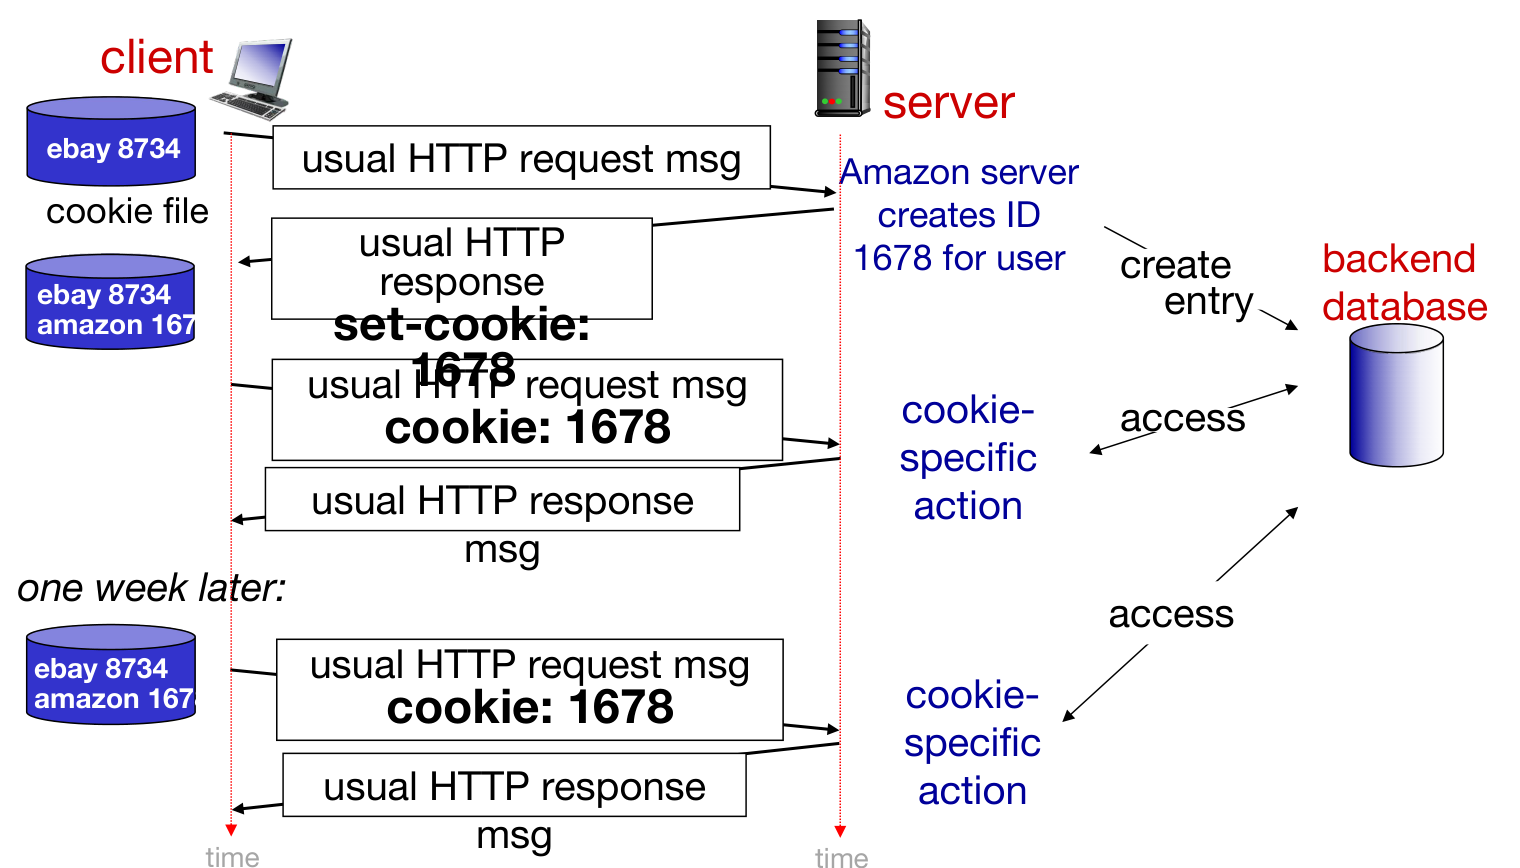
\includegraphics[width=.92\textwidth]{ch06-cookie.png}
\caption{Cookie事件顺序：服务器首次分配标识并写入后台记录，浏览器保存标识，后续请求带回Cookie供服务器查找状态。来源：\texttt{Chapter6-应用层.pdf}，PDF第86页（显示页86），局部截取。}
\end{figure}

\annotationarea[4]
\small 来源：\texttt{Chapter6-应用层.pdf}，PDF阅读器第51--87页（显示页51--87）；参考书PDF第300--313页（印刷第289--302页）。课件缓存算例与RTT公式均在正文列出假设并给出计算过程。\normalsize

\section{P2P应用与文件分发}
\subsection{客户机/服务器与P2P分发时间}
设文件大小为$F$ bit，要分发给$N$个节点。服务器上传速率为$u_s$ bit/s，第$i$个节点上传速率为$u_i$，下载速率为$d_i$，最慢下载速率为$d_{\min}=\min_i d_i$。分发时间至少要满足文件数据能够从发送端上传、每个节点能下载完整文件这两个基本条件。

\textbf{客户机/服务器分发。}服务器至少要上传$N$份文件，共$NF$ bit；最慢客户至少需要$F/d_{\min}$秒下载一份。因此
\[
D_{\mathrm{C/S}}\geq \max\left\{\frac{NF}{u_s},\frac{F}{d_{\min}}\right\}.
\]
当$N$增大时，服务器上传项$NF/u_s$线性增加，服务器可能成为瓶颈。

\textbf{P2P分发。}服务器至少上传一份文件；每个节点仍须下载完整文件；服务器和所有节点合起来至少要上传总计$NF$ bit。因此
\[
D_{\mathrm{P2P}}\geq \max\left\{\frac{F}{u_s},\frac{F}{d_{\min}},
\frac{NF}{u_s+\sum_{i=1}^{N}u_i}\right\}.
\]
第三项体现P2P节点可以贡献上传能力。这里是理论下界；实际完成时间还受节点在线情况、带宽共享和协议调度等因素影响。

\textbf{课件参数例（PDF第93页）。}设每个节点上传速率为$u$，服务器上传速率$u_s=10u$，最慢下载速率$d_{\min}\geq u_s$，且$F/u=1$小时。取$N=100$：
\[
D_{\mathrm{C/S}}\geq\max\{100F/(10u),F/d_{\min}\}=\max\{10,\leq0.1\}\text{小时}=10\text{小时}.
\]
P2P下$\sum_i u_i=100u$，所以
\[
D_{\mathrm{P2P}}\geq\max\left\{0.1,\leq0.1,\frac{100F}{110u}\right\}
\text{小时}\approx0.91\text{小时}.
\]
两式是下界比较，说明当用户多、对等节点能贡献上传时，P2P不必像C/S那样由一个服务器承担全部副本；它不保证任意网络实际用时都恰好等于该下界。

\subsection{BitTorrent文件交换}
课件用\textbf{BitTorrent}说明P2P文件交换。一个文件被切成固定大小的块（chunk），课件示例大小为256 KB；正在交换同一文件块的一组节点称为一个\textbf{torrent}。\textbf{Tracker}记录参与torrent的节点，帮助新节点取得邻居列表，但实际文件块在peer之间交换。

\begin{figure}[H]\centering
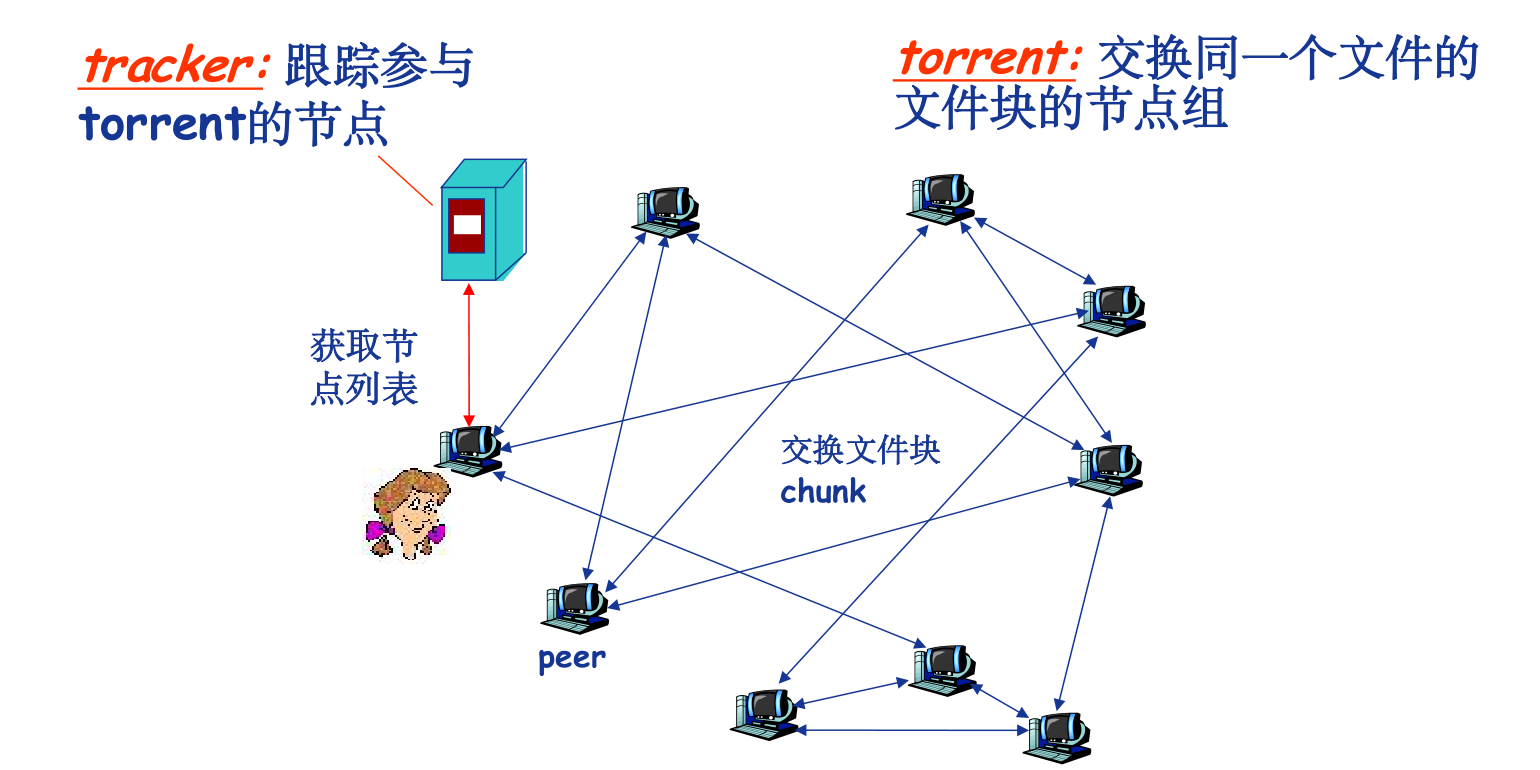
\includegraphics[width=.86\textwidth]{ch06-bittorrent.png}
\caption{Tracker帮助新peer取得参与节点列表；蓝色箭头表示peer之间交换文件块，而非经Tracker中转。来源：\texttt{Chapter6-应用层.pdf}，PDF第94页（显示页94），局部截取。}
\end{figure}

新节点加入时还没有文件块，先向Tracker登记并取得节点清单，再连接其中一些邻居。节点下载的同时也向其他节点上传；节点可以加入或离开。节点定期查询邻居持有的块列表，并向邻居请求自己缺少的块。课件列出的\textbf{稀缺优先（rarest first）}原则是优先请求当前较少见的块，避免稀有块只留在少数节点上。

\textbf{Tit-for-tat（以牙还牙）}用上传合作鼓励互惠：Alice优先向当前给她较快上传的4个邻居提供块，并每10秒重新评估；此外每30秒随机选一个其他节点试传块，这称为\textbf{乐观解封（optimistic unchoke）}。随机试传可能发现更好的交换伙伴，双方随后都能进入对方的较快上传邻居集合。节点取得完整文件后可以离开，也可以留下继续上传。

\begin{figure}[H]\centering
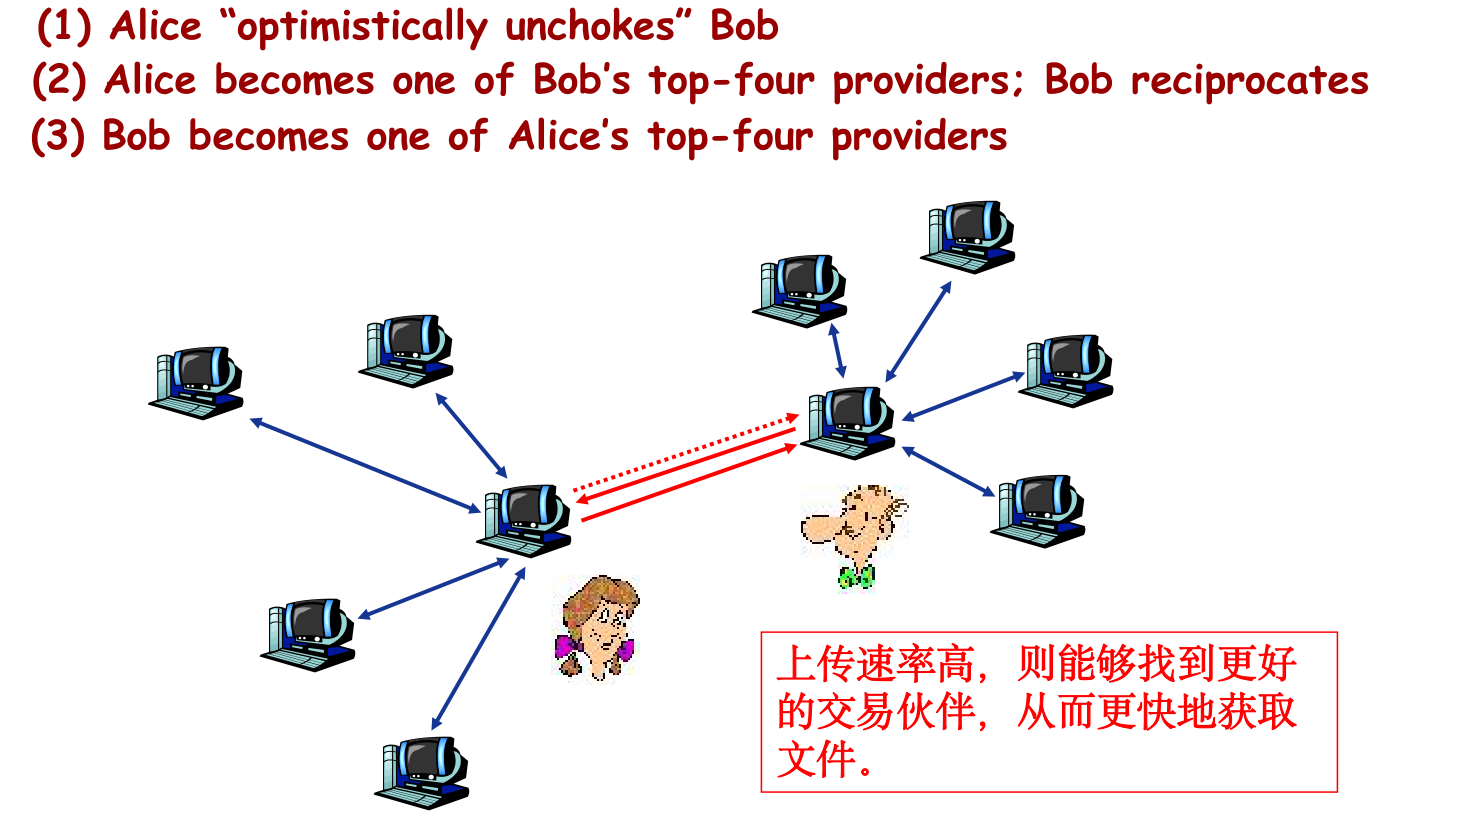
\includegraphics[width=.90\textwidth]{ch06-bittorrent-unchoke.png}
\caption{乐观解封建立新的试传机会；如果互相上传后成为对方较快的前四个提供者，双方会继续互惠。来源：\texttt{Chapter6-应用层.pdf}，PDF第97页（显示页97），局部截取。}
\end{figure}

\subsection{P2P索引与分布式哈希表}
P2P应用还需要解决“内容在哪里”的问题。\textbf{索引}是从内容或用户名映射到节点位置（IP地址与端口号）的信息。课件比较了集中式索引、洪泛式查询、层次式覆盖网络和分布式哈希表。

\begin{itemize}[nosep]
\item \textbf{集中式索引：}Napster中节点加入时向中央目录登记IP地址和共享内容；Alice查询文件名后，目录返回持有文件的节点，Alice再直接向该节点请求文件。目录单点故障或过载会影响查找；内容和文件传输虽分布在节点之间，定位仍集中。
\item \textbf{洪泛式查询（query flooding）：}Gnutella例中，每个节点只索引自己共享的文件；活动节点之间的TCP连接构成覆盖网络（overlay network），其边是逻辑上的虚拟链路。查询沿已有连接向邻居扩散；若某节点命中，就沿查询来路返回QueryHit；随后文件可由节点间传输。洪泛无需中央索引，但可能产生较多查询消息。
\item \textbf{层次式覆盖网络：}部分节点充当超级节点，普通节点连接某个超级节点，超级节点之间也可连接。超级节点跟踪所辖节点的内容，形成介于集中式索引与完全洪泛之间的组织方式。
\item \textbf{分布式哈希表（Distributed Hash Table，DHT）：}把键值对分散存放在众多peer上；查询给出key，系统返回匹配的value，节点也能插入键值对。
\end{itemize}

DHT把原始key通过哈希函数转成整数，并给peer也分配相同范围内的整数标识符。若标识符用$n$ bit表示，范围为$[0,2^n-1]$。课件约定把key分配给\textbf{顺时针方向遇到的第一个peer（successor）}。例如$n=4$、peer标识为$1,3,4,5,8,10,12,14$：key 13由peer 14负责；key 15顺时针绕回后由peer 1负责。

\textbf{环形DHT查找。}若每个peer只知道直接后继和前驱，查询会沿环逐个转发，课件给出的平均消息数为$O(N)$。增加shortcut（快捷连接）后，一个peer可按规则跳到更远节点；课件说明可用$O(\log N)$个邻居把查找消息数降至$O(\log N)$。图中红色箭头表示key 1110从发起peer沿快捷路径转发并交给顺时针后继。

\begin{figure}[H]\centering
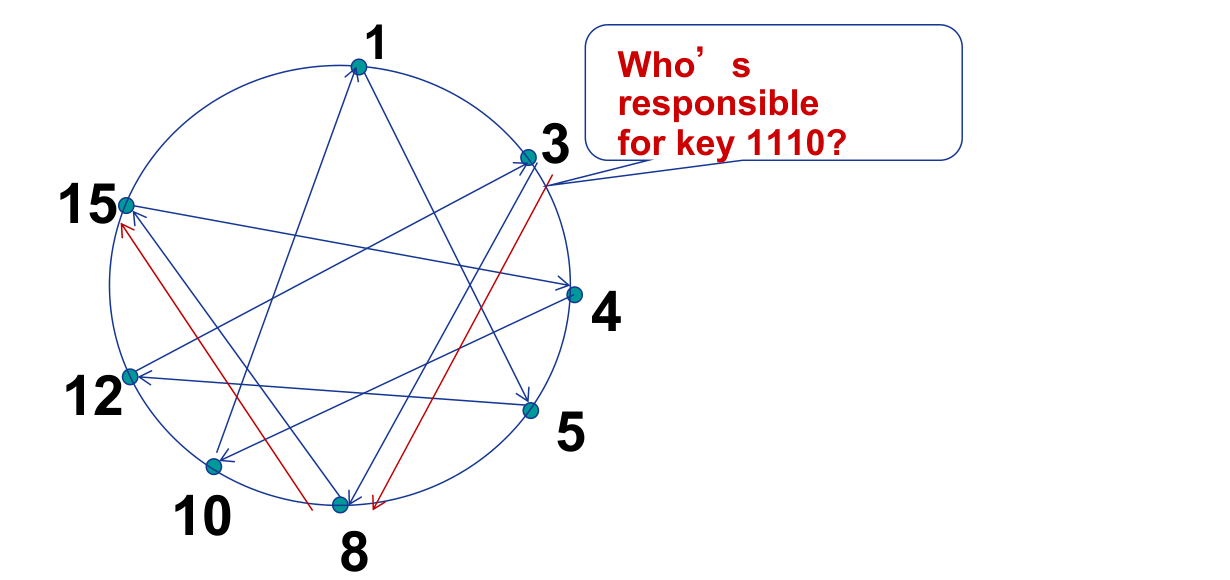
\includegraphics[width=.76\textwidth]{ch06-dht-ring.png}
\caption{环形DHT及快捷连接示意：蓝色边是peer间覆盖连接，红色箭头展示key查询的转发方向；按顺时针后继确定负责该key的peer。来源：\texttt{Chapter6-应用层.pdf}，PDF第111页（显示页111），局部截取。}
\end{figure}

\textbf{节点动态变化（peer churn）。}P2P节点会加入、离开或突然失效。课件示例让每个peer记住两个后继并定期ping它们；若直接后继失效，就把第二后继提升为新的直接后继，再询问它的后继以补足列表。例如peer 5离开后，peer 4把peer 8设为直接后继，并向peer 8询问下一个后继。维护后继列表可降低单个节点失效导致环断裂的风险。

\annotationarea[4]
\small 来源：\texttt{Chapter6-应用层.pdf}，PDF阅读器第89--112页（显示页89--112）。教材PDF第278--280页（印刷第267--269页）核对C/S与P2P模型；文件分发公式、BitTorrent、覆盖网络和DHT按课件整理。\normalsize

\section{Socket API与TCP调用流程}
\subsection{API、套接字描述符与地址}
\textbf{应用编程接口（Application Programming Interface，API）}是应用进程调用操作系统功能的接口。课件用Socket API说明应用程序如何创建通信端点、设置地址、建立TCP连接、发送和接收数据。套接字对外由IP地址和端口标识；对进程内部，操作系统返回一个小整数\textbf{套接字描述符（socket descriptor）}，应用通过它引用套接字。

创建套接字时，操作系统为它保存协议族、服务类型、本地和远端IP及端口等信息。课件给出的IPv4地址结构\texttt{sockaddr\_in}包括地址长度\texttt{sin\_len}、地址族\texttt{sin\_family}（TCP/IP使用\texttt{AF\_INET}）、端口\texttt{sin\_port}、IP地址\texttt{sin\_addr}以及未用字段\texttt{sin\_zero}。不同操作系统的结构定义略有差异，实际编程应以当前平台头文件为准；学习时重点识别地址族、端口和IP地址。

\subsection{常用Socket API函数}
课件以WinSock（Windows Socket Interface）为例。\texttt{WSAStartup}初始化WinSock库，\texttt{WSACleanup}结束使用并释放库资源；它们只用于WinSock。课件示例以\texttt{MAKEWORD(2,1)}请求2.1版，并用\texttt{WSADATA}取得实际版本信息。

\begin{center}\begin{tabularx}{.98\textwidth}{lXX}\toprule
函数 & 作用 & 使用场景 \\\midrule
\texttt{socket} & 创建套接字并返回描述符 & \texttt{PF\_INET}指定IPv4族；\texttt{SOCK\_STREAM}用于TCP，\texttt{SOCK\_DGRAM}用于UDP，\texttt{SOCK\_RAW}为原始套接字 \\
\texttt{bind} & 把本地IP和端口绑定到套接字 & 服务器通常绑定熟知端口；需接收多个本地接口的请求时可用\texttt{INADDR\_ANY} \\
\texttt{listen} & 让流套接字进入监听状态并设连接请求队列大小 & 服务器端TCP套接字 \\
\texttt{connect} & 指定要通信的远端地址 & TCP客户端建立连接；UDP客户端指定默认对端，不进行TCP式握手 \\
\texttt{accept} & 从监听队列取出一个TCP连接请求并返回新的连接套接字 & 服务器端TCP；监听套接字继续接受其他客户 \\
\texttt{send}/\texttt{recv} & 发送/接收字节或数据 & TCP，以及已调用\texttt{connect}的UDP客户端 \\
\texttt{sendto}/\texttt{recvfrom} & 发送/接收数据报并指定/取得对端地址 & 未连接的UDP套接字 \\
\texttt{closesocket} & 关闭或释放套接字描述符 & 使用结束时调用 \\
\texttt{setsockopt}/\texttt{getsockopt} & 设置/读取套接字选项 & 调整或查询套接字行为参数 \\\bottomrule\end{tabularx}\end{center}

服务器通常需要\texttt{bind}到服务端口。多网卡服务器若要在所有IPv4本地接口接收连接，可使用地址通配符\texttt{INADDR\_ANY}。客户端通常无需手动\texttt{bind}，系统可自动选择本地IP和临时端口。TCP服务器的\texttt{listen}负责排队等候请求，\texttt{accept}从队列中取出一个请求，并创建新的连接套接字供该客户使用。

课件给出的\texttt{send}、\texttt{recv}等函数原型是说明参数角色的示意形式，不是适用于所有系统的完整可编译签名。TCP是字节流，接收一次数据不一定与对方一次发送的边界一一对应；UDP则按数据报接收，并通过\texttt{sendto}/\texttt{recvfrom}携带对端地址。

\subsection{TCP客户端与服务器的调用次序}
\begin{figure}[H]\centering
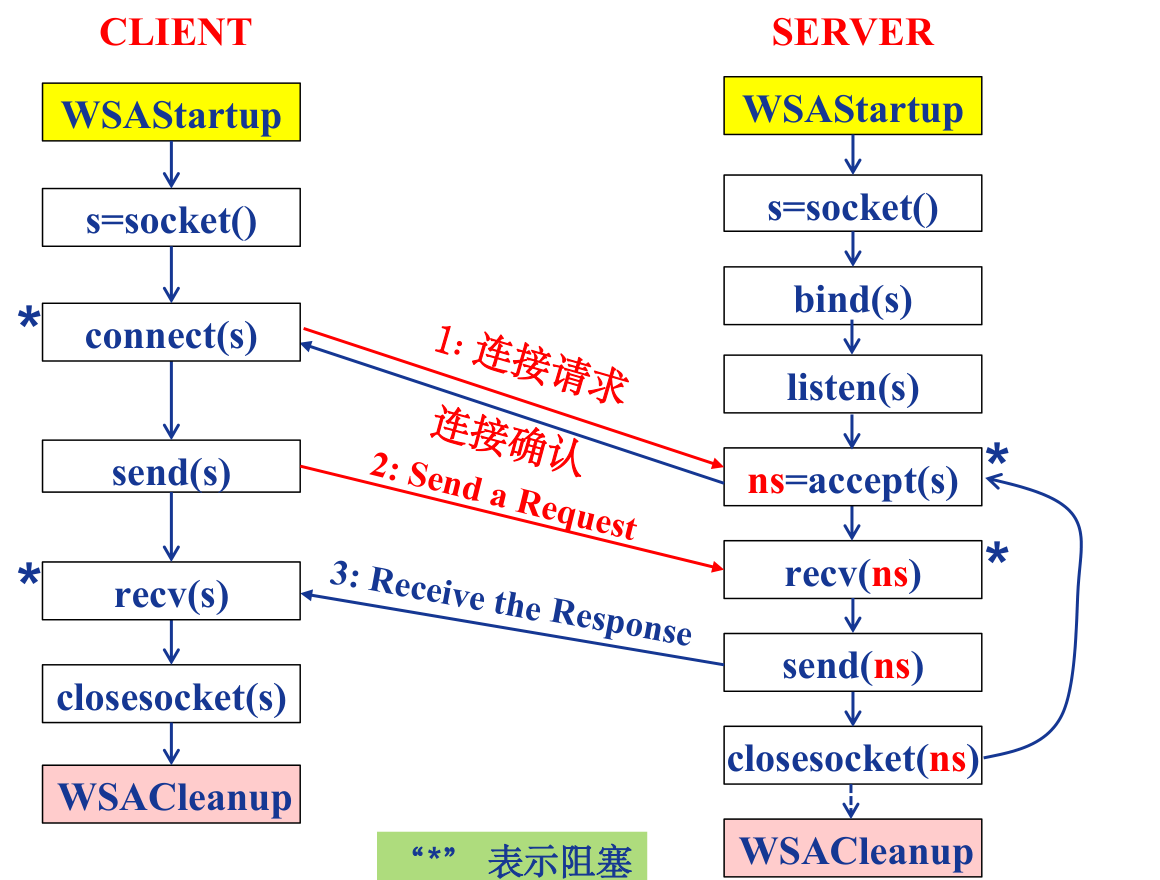
\includegraphics[width=.88\textwidth,height=.68\textheight,keepaspectratio]{ch06-socket-flow.png}
\caption{WinSock TCP基本调用流程：服务器创建、绑定并监听，\texttt{accept}等待连接；客户端\texttt{connect}发起连接后发送请求、接收响应。星号表示可能阻塞等待。来源：\texttt{Chapter6-应用层.pdf}，PDF第137页（显示页137），局部截取。}
\end{figure}

按图读一次请求/响应：
\begin{enumerate}[nosep]
\item 客户端和服务器先分别调用\texttt{WSAStartup}，再各自用\texttt{socket}创建套接字。
\item 服务器用\texttt{bind}绑定服务地址和端口，用\texttt{listen}进入监听，再调用\texttt{accept}等待客户；\texttt{accept}返回新的套接字\texttt{ns}。
\item 客户端调用\texttt{connect}连接服务器；服务器收到请求后，\texttt{accept}解除阻塞并返回\texttt{ns}。
\item 客户端通过\texttt{send}发送请求，服务器在\texttt{recv(ns)}取得数据，处理后用\texttt{send(ns)}返回响应。
\item 客户端用\texttt{recv}接收响应；双方分别用\texttt{closesocket}关闭各自连接端点，最后调用\texttt{WSACleanup}。
\end{enumerate}

图中的监听套接字与连接套接字用途不同：监听套接字负责等待更多连接；\texttt{accept}产生的连接套接字负责和某一个客户交换数据。标有星号的\texttt{connect}、\texttt{accept}、\texttt{recv}可能在条件未满足时阻塞等待。

\subsection{网络字节顺序}
网络协议首部中的多字节整数使用统一的\textbf{网络字节顺序（network byte order）}表示。主机内部的本地字节顺序可能不同，向Socket API传递端口或IP数值前后需转换：\texttt{htons}把16位本地值转成网络顺序，\texttt{ntohs}反向转换；\texttt{htonl}和\texttt{ntohl}分别处理32位值。端口号是16位，IPv4地址是32位。

\textbf{Socket API基础调用练习。}假设服务器TCP端口为80，客户端要发送一次HTTP请求。服务器先创建流套接字、绑定80号端口并监听；客户端创建流套接字并\texttt{connect}服务器IP与80号端口；服务器\texttt{accept}并取得专用连接套接字；客户端\texttt{send}请求，服务器\texttt{recv}请求并\texttt{send}响应，客户端\texttt{recv}响应；最后双方关闭连接套接字。注意：客户端的本地端口由系统分配；服务器原有监听套接字不因处理这一客户而变成该连接的通信套接字。

\annotationarea[4]
\small 来源：\texttt{Chapter6-应用层.pdf}，PDF阅读器第114--137页（显示页114--137）。课件第113页将6.8标为“略”，但后续页面仍给出API概念、结构、函数和TCP调用流程；本节据实际页面整理这些基础内容，不扩展成语言编程教程。\normalsize

\section*{本章复习与自检}
\begin{enumerate}[nosep]
\item 解释C/S与P2P在请求、服务提供和文件传输中的区别；Napster混合结构的搜索与传输分别由谁完成？
\item 若主机已知道域名但本地DNS缓存未命中，说明本地DNS服务器采用迭代查询时的查询顺序；区别递归查询与迭代查询。
\item FTP控制连接和数据连接分别传什么？为什么图中服务器20号端口不能解释为所有模式都必用？
\item 说明SMTP、POP3/IMAP分别负责邮件流程的哪一段；解释MIME为什么不取代SMTP。
\item 对比HTTP/1.0非持久连接、HTTP/1.1持久连接与流水线、HTTP/2帧交错和HTTP/3的QUIC流。
\item 给出P2P文件分发下界中三项分别限制了什么；在DHT中说明key 15由谁负责。
\item 写出TCP服务器和客户端的Socket API主要调用顺序，并解释为什么服务器要区分监听套接字和\texttt{accept}返回的连接套接字。
\end{enumerate}
\textbf{自检答案要点：}Napster由中央目录登记和搜索、节点直传文件；迭代查询由本地DNS逐级询问并根据转介继续，递归查询由被问服务器代办后续；FTP控制连接传命令、数据连接传文件，20号是主动模式示例；SMTP负责推送发送、POP3/IMAP负责读取，MIME提供内容编码与格式扩展；非持久连接每对象建连接，持久连接复用，HTTP/2交错帧但共享TCP仍可能因丢包一起等待，QUIC按流隔离可靠传输；P2P三项分别对应服务器首份上传、最慢节点下载、全系统总上传能力，key15顺时针绕回由peer1负责；服务器序列为socket-bind-listen-accept-send/recv，客户端为socket-connect-send/recv。

\small 来源：本节综合\texttt{Chapter6-应用层.pdf}第4--137页。参考书核对范围：PDF第278--313页（印刷第267--302页）；P2P文件分发、DHT和Socket API详细内容以课件为准。\normalsize

\chapter{无线与移动网络}

\noindent\textbf{本章要解决的问题。} 有线网络中的主机通常通过固定链路接入；无线网络则让主机借助无线电链路通信，但信号会衰减、受干扰，还可能在接收端发生发送者彼此听不到的冲突。移动网络还要解决另一个问题：设备改变接入点或运营商网络后，数据怎样继续找到它。本章依课件顺序学习无线网络概述、无线链路特性、IEEE 802.11 无线局域网、蜂窝网络结构、网络移动管理、移动 IP、蜂窝网切换以及无线对高层协议的影响。

\section{无线与移动网络概述}
\subsection{无线与移动是两个不同概念}
\textbf{无线}表示通信链路使用无线电等非有线介质；\textbf{移动}表示设备在网络接入点之间移动时，网络仍要处理其位置变化。一个设备可以是无线但静止的，例如固定安装的无线传感器；也可以移动但暂时关闭无线通信。因此“无线网络”和“移动网络”关注的挑战不同：前者要解决无线链路上的传输和共享问题，后者要解决接入点改变后如何维持连接与寻址。

\textbf{无线主机}是运行应用程序并通过无线链路收发数据的终端，例如笔记本电脑、智能手机和物联网设备。\textbf{基站}通常连接到有线网络，在其覆盖范围内中继无线主机与有线网络之间的数据；蜂窝网络中的基站和 Wi-Fi 中的接入点都承担类似角色。\textbf{无线链路}可以连接主机与基站，也可以连接网络中的其他节点；多个主机共享链路时，需要多路访问控制协议协调谁在何时发送。

\subsection{无线网络的两种组织方式}
\textbf{基础设施模式}中，无线主机先连接基站，再由基站接入更大的有线网络。无线主机从一个基站换到另一个基站称为\textbf{切换}（handoff/handover）；切换期间网络需要更新接入关系。\textbf{特定网模式}（ad hoc，自组网）没有预先部署的基站，节点自行组织网络；若目的节点不在直接无线覆盖范围内，中间节点还要转发数据，兼任终端和路由节点。

课件还用两个维度分类无线网络：是否有基础设施、通信需经过几跳。基础设施单跳网络如普通 Wi-Fi，主机经接入点（AP，Access Point）接入互联网；无基础设施单跳网络如近距离点对点连接；多跳网络让数据经过多个无线节点中继。基础设施多跳网络可形成无线网状网络；无基础设施多跳网络包括移动自组网（MANET，Mobile Ad Hoc Network）和车载自组网（VANET，Vehicular Ad Hoc Network）。这些名称描述网络组织方式，不代表所有这类网络必然具有同一套路由协议。

课件以 2019 年的用户与宽带连接比例说明无线接入的重要性。这些数字是课件所用的历史背景数据，不应当作当前统计值。参考教材把无线归入传输介质和局域网等章节，本节的网络分类、结构图以课件为主。
\annotationarea[4]
\small 来源：课件 \texttt{Chapter7-无线与移动网络.pdf}，PDF阅读器第4--12页（对应显示页4--12）；无线介质概念参考《2027年计算机网络考研复习指导》第2章§2.2.1，PDF第53--55页（印刷第42--44页）。\normalsize

\section{无线链路与网络特性}
\subsection{衰减、干扰与多径传播}
无线电波在传播过程中能量会随距离和环境减弱，这称为\textbf{路径损耗}。障碍物、墙体和距离变化都会让接收信号强度改变。多个设备可能使用相同或相邻频段，产生\textbf{干扰}。无线信号还可能被墙壁、地面或物体反射，沿不同路径、在不同时间到达接收端，这称为\textbf{多径传播}。多条路径上的信号叠加后可能增强，也可能互相抵消，因而接收质量会随位置和时间变化。

\textbf{信噪比}（SNR，Signal-to-Noise Ratio）描述有用信号相对于噪声的强弱；信噪比越高，通常越容易从噪声中恢复信号。\textbf{误码率}（BER，Bit Error Rate）是传输中错误比特占总比特的比例。给定物理层方案时，提高发射功率通常能提高 SNR、降低 BER；给定 SNR 时，调制方式越复杂通常能承载更高速率，但要满足更低的误码要求。设备会根据链路质量调整调制方式和速率：链路变差时改用较低速率以降低误码，链路变好时再尝试较高速率。

\subsection{隐藏终端与信号衰减}
无线节点的可侦听范围和接收端的覆盖范围不一定相同。\textbf{隐藏终端问题}是指两个发送端彼此听不到，却都能到达同一个接收端。例如 A 和 C 都能与 B 通信，但 A、C 互相听不到；二者若同时给 B 发送，信号会在 B 处冲突。\textbf{信号衰减导致的冲突}也会产生相同后果：A、C 的信号分别足以到达 B，但在对方所在位置已经弱到无法侦听，于是它们误以为信道空闲。

\begin{figure}[H]\centering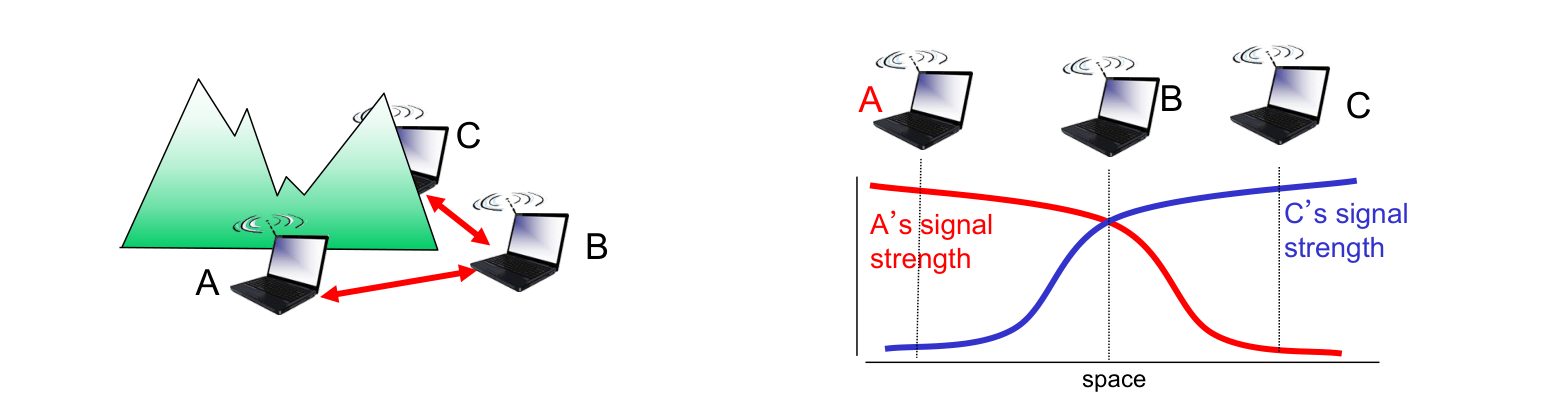
\includegraphics[width=.91\textwidth]{ch07-hidden-terminal.png}\caption{隐藏终端与信号衰减示意：A、C 各自能到达 B，却无法互相侦听；右侧曲线表示两发送端信号强度随位置变化。来源：\texttt{Chapter7-无线与移动网络.pdf}，PDF阅读器第16页（显示页16），局部截取。}\label{fig:ch07-hidden-terminal}\end{figure}

这说明无线节点只监听自己位置的信道，不能保证知道接收端是否会发生冲突；无线网卡也难以像有线以太网那样边发送边检测所有冲突。IEEE 802.11 因而采用冲突避免和确认重传机制，尽量减少冲突并判断帧是否成功到达。
\annotationarea[4]
\small 来源：课件PDF阅读器第14--16页（显示页14--16）；参考教材第3章§3.6.3，PDF第104--107页（印刷第93--96页），用于核对无线信道、隐藏站与CSMA/CA机制。\normalsize

\section{无线局域网：802.11 标准}
\subsection{802.11 标准与基本服务集}
IEEE（Institute of Electrical and Electronics Engineers，电气电子工程师学会）802.11 是无线局域网标准族，常见产品通常称 Wi-Fi。不同版本在频段、物理层技术和最高数据率方面不同。\textbf{直接序列扩频}（DSSS，Direct Sequence Spread Spectrum）把数据扩展到较宽的码片序列；\textbf{正交频分复用}（OFDM，Orthogonal Frequency Division Multiplexing）把数据并行映射到相互正交的多个子载波；\textbf{多输入多输出}（MIMO，Multiple-Input Multiple-Output）使用多根发射、接收天线提高传输能力。表中数据是课件列出的速率和距离，实际速率与覆盖范围会受设备、信道带宽、干扰及环境影响。

\begin{center}\small
\begin{tabularx}{.98\textwidth}{l l l X}\toprule
课件列出的版本 & 频段 & 最高速率 / 距离（课件值） & 课件强调的物理层特点 \\\midrule
802.11b & 2.4--2.5 GHz & 11 Mb/s / 约30 m & DSSS；课件称成本低、传播距离较远 \\
802.11a & 5--6 GHz & 54 Mb/s / 约30 m & OFDM；速率较高、覆盖相对短 \\
802.11g & 2.4--2.5 GHz & 54 Mb/s / 约30 m & OFDM \\
802.11n（Wi-Fi 4） & 2.4/5 GHz & 600 Mb/s / 约70 m & MIMO 与 OFDM；课件提到40 MHz带宽 \\
802.11ac（Wi-Fi 5） & 5 GHz & 约3.47 Gb/s / 约70 m & 课件表列值 \\
802.11ax（Wi-Fi 6） & 2.4/5 GHz & 约14 Gb/s / 约70 m & 课件表列值 \\
802.11af / ah & 54--790 MHz / 约900 MHz & 35--560 / 347 Mb/s；约1 km & 课件强调较远距离 \\\bottomrule
\end{tabularx}\end{center}

课件第18页对 802.11b/a/g/n 还列出了最高数据率及频段；第20页扩展了版本和距离表。表内“2020（exp.）”等年代与速率应理解为课件资料的记录时点，不用于推断今天的部署情况。课件称这些 Wi-Fi 网络既可工作于基础设施模式，也可工作于自组网模式，并采用 CSMA/CA（Carrier Sense Multiple Access with Collision Avoidance，载波监听多路访问/冲突避免）进行多路访问。802.11b 的课件说明还指出同一网络中的主机使用相同的扩频码片序列。

基础设施模式中的基站称为\textbf{接入点}（AP，Access Point）。一个\textbf{基本服务集}（BSS，Basic Service Set）是一个 AP 及与它通信的无线主机所组成的局部网络，课件也称其为一个 cell。主机要先选择并关联到 AP，之后才能通过该 AP 接入更大的网络。课件还画出没有 AP、只有主机组成的 ad hoc 网络。

\subsection{信道选择、扫描与关联}
无线频谱被分成不同信道，AP 选择信道工作；相邻 AP 若选用相同或相邻信道，可能互相干扰。主机通过扫描发现 AP：AP 的信标帧（beacon）包含网络名称\textbf{服务集标识符}（SSID，Service Set Identifier）及 AP 的 MAC 地址。主机选定 AP 后发起关联；网络可能还要进行身份认证。成功接入局域网后，主机通常通过\textbf{动态主机配置协议}（DHCP，Dynamic Host Configuration Protocol）获得 IP 地址等配置。

课件区分两种扫描过程：\textbf{被动扫描}中，各 AP 周期性发送信标，主机监听并选择 AP，再发送关联请求，AP 返回关联响应；\textbf{主动扫描}中，主机先广播探测请求（Probe Request），AP 回探测响应（Probe Response），之后主机发送关联请求、AP 返回关联响应。两种方式都是先发现候选 AP，再完成关联；主动扫描多出探测请求/响应这一对报文。

\begin{figure}[H]\centering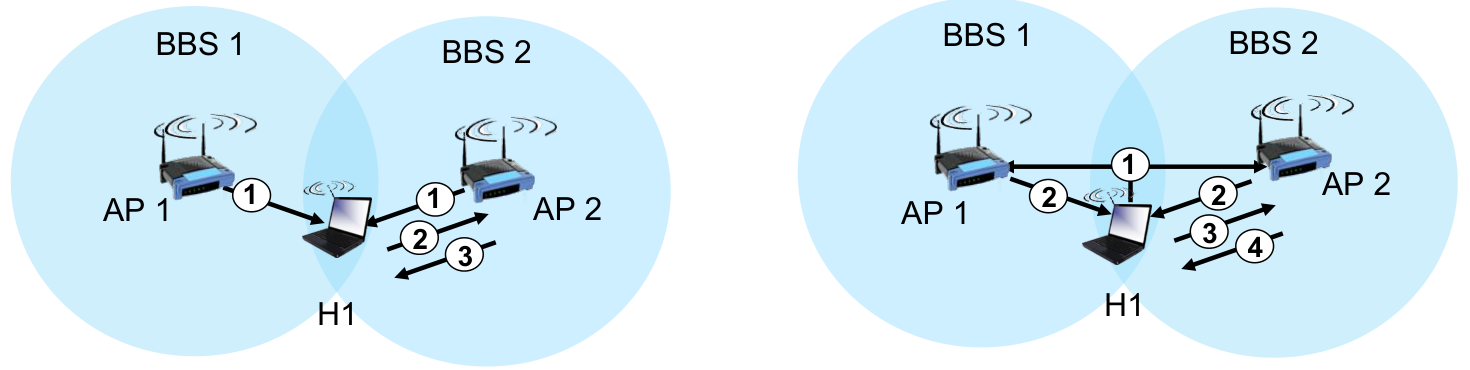
\includegraphics[width=.93\textwidth]{ch07-wifi-scan.png}\caption{被动与主动扫描：左边 AP 主动发送信标，右边主机先发 Probe Request；圆圈编号表示报文事件次序。来源：\texttt{Chapter7-无线与移动网络.pdf}，PDF阅读器第23页（显示页23），局部截取。}\label{fig:ch07-wifi-scan}\end{figure}
\annotationarea[4]

\subsection{CSMA/CA 与 RTS/CTS 信道预约}
CSMA（Carrier Sense Multiple Access，载波监听多路访问）要求发送前先监听信道。有线以太网的 CSMA/CD（Carrier Sense Multiple Access with Collision Detection，载波监听多路访问/冲突检测）可以在发送时检测碰撞并停止发送；802.11 无线网很难在强发送信号旁检测微弱接收信号，而且隐藏终端使发送端看不到接收端处的所有碰撞，因此使用 CSMA/CA（Carrier Sense Multiple Access with Collision Avoidance，载波监听多路访问/冲突避免）。“避免”是降低冲突概率，不保证冲突绝不发生。

课件描述的发送端规则如下：
\begin{enumerate}[nosep]
  \item 若信道空闲持续一个 DIFS（Distributed Inter-Frame Space，分布式协调帧间间隔）时间，发送整个帧。发送过程中不做冲突检测。
  \item 若信道忙，或上次未收到确认，选取随机退避时间。信道空闲时退避计时器递减；信道变忙时计时器暂停，等重新空闲后再继续。
  \item 计时器到零时发送帧。接收方正确收到帧后，等待更短的 SIFS（Short Inter-Frame Space，短帧间间隔）再回 ACK（Acknowledgment，确认帧）。SIFS 短于 DIFS，使当前数据交换中的 ACK 优先于新的竞争发送。
  \item 若发送端没有收到 ACK，就认为帧可能丢失或冲突，扩大随机退避间隔后重试。
\end{enumerate}

\begin{figure}[H]\centering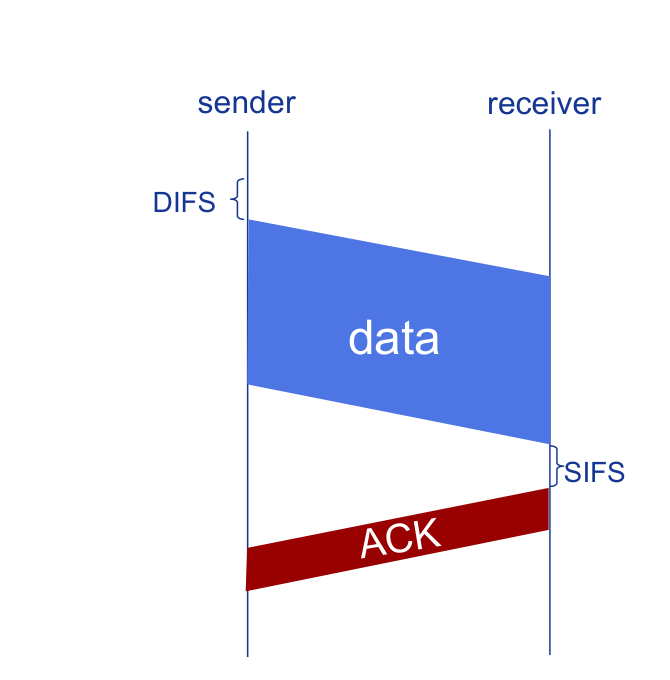
\includegraphics[width=.56\textwidth]{ch07-csma-ca-timing.png}\caption{CSMA/CA 发送时序：发送端等待 DIFS 后发送数据，接收端再等待 SIFS 并回 ACK。图中横向为时间，纵向两条线分别表示发送端和接收端。来源：\texttt{Chapter7-无线与移动网络.pdf}，PDF阅读器第25页（显示页25），局部截取。}\label{fig:ch07-csma-ca-timing}\end{figure}

当隐藏终端较明显时，可用请求发送帧 RTS（Request To Send）和允许发送帧 CTS（Clear To Send）预约信道。发送端先按 CSMA 规则竞争并发送 RTS；接入点正确收到后，经 SIFS 返回 CTS。周围节点能听到 CTS 后会推迟发送，随后发送端经 SIFS 发送数据，接收端再经 SIFS 返回 ACK。RTS 本身仍可能冲突，但它短于数据帧，因此冲突造成的浪费较小。RTS/CTS 是可选的预约办法，不表示无线冲突从此完全消失。

\textbf{网络分配向量}（NAV，Network Allocation Vector）是节点根据帧中的 Duration（持续期）字段设置的虚拟忙碌计时器。即使节点没有听到隐藏发送端的 RTS，只要它听到接入点发出的 CTS，就能从持续期字段知道应暂缓发送多久。物理载波监听是实际检测无线信号；NAV 是按收到的预约通知推算信道将被占用的时间。

\begin{figure}[H]\centering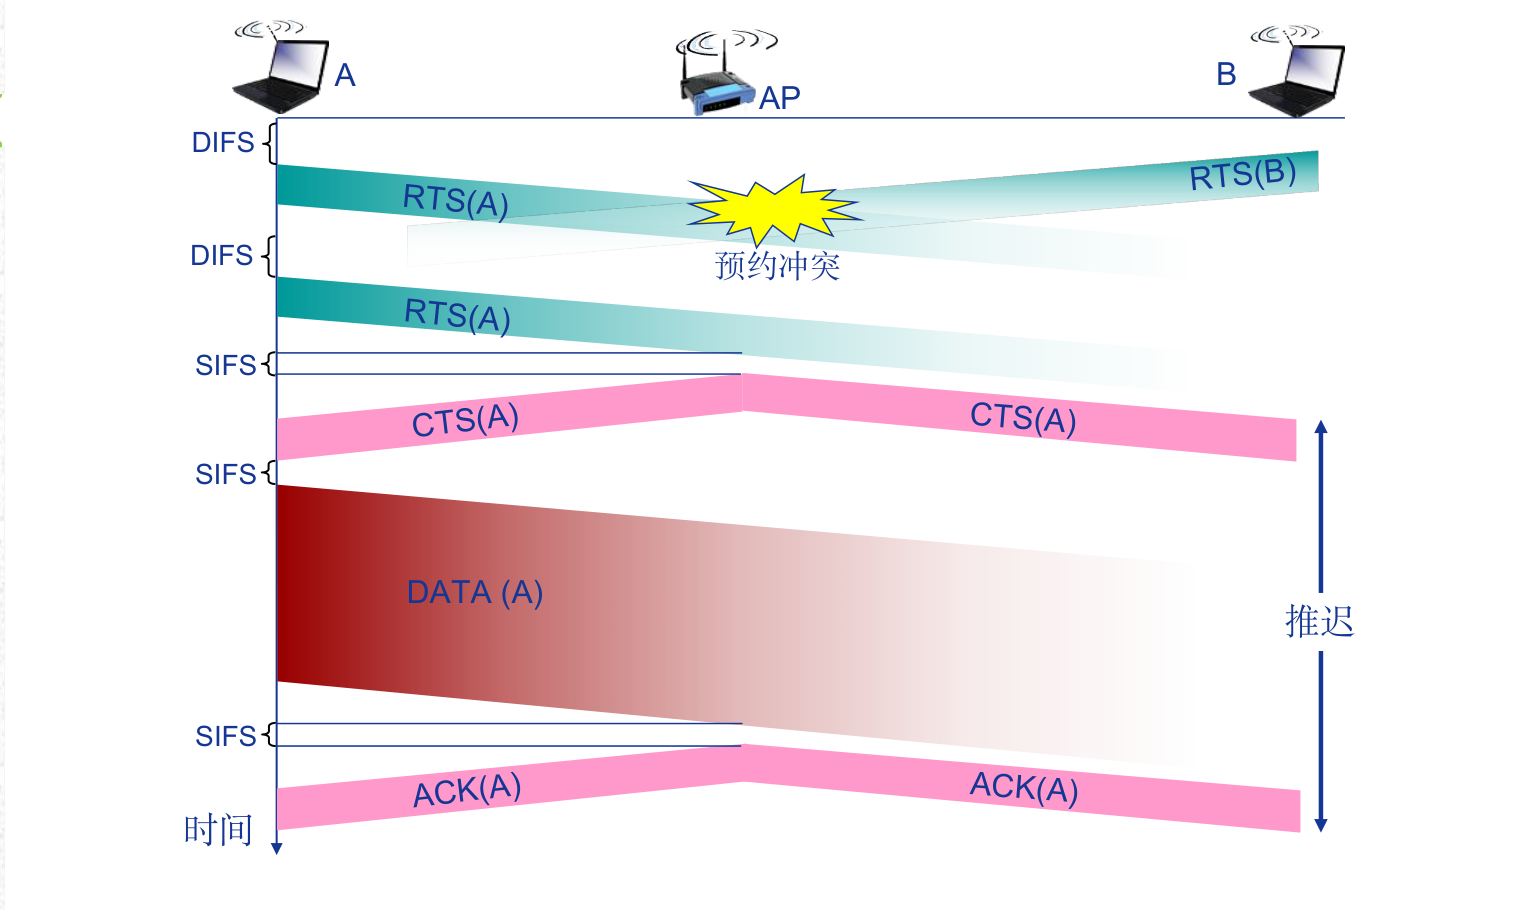
\includegraphics[width=.91\textwidth]{ch07-rts-cts.png}\caption{RTS/CTS 预约时间线：A 与 B 的 RTS 可发生冲突；接入点收到 A 的 RTS 后回 CTS，B 听到 CTS 后推迟，A 再发送 DATA 并收到 ACK。横向箭头为时间，纵向为不同节点。来源：\texttt{Chapter7-无线与移动网络.pdf}，PDF阅读器第27页（显示页27），局部截取。}\label{fig:ch07-rts-cts}\end{figure}

\textbf{课件例题（PDF第28页）：} 忽略传播、处理及所有帧的发送时间，某主机从希望发送开始，到收到接收正确的确认帧，最快需要多久？假设信道空闲且不需要随机退避。

\textbf{解：} 从希望发送到收到确认，按事件顺序是：发送端先等待 DIFS，再发 RTS；接收端收到 RTS 后等待第一个 SIFS，再回 CTS；发送端收到 CTS 后等待第二个 SIFS，再发 DATA；接收端收到 DATA 后等待第三个 SIFS，再回 ACK。题目让忽略 RTS、CTS、DATA、ACK 的发送时间，以及传播和处理时间，所以只把帧间等待相加：第一个控制帧前的 DIFS，加上 RTS--CTS、CTS--DATA、DATA--ACK 三个相邻帧间的 SIFS。
\[
  T_{\min}=\mathrm{DIFS}+3\,\mathrm{SIFS}.
\]
若信道一开始忙或产生冲突，就还要加上推迟接入和随机退避时间；题目所给假设排除了这些等待。
\annotationarea[4]
\small 来源：课件PDF阅读器第24--28页（显示页24--28）；参考教材第3章§3.6.3，PDF第105--107页（印刷第94--96页），核对DIFS/SIFS、随机退避、ACK、NAV及RTS/CTS过程。\normalsize

\subsection{802.11 MAC 帧及地址字段}
MAC（媒体访问控制，Medium Access Control）帧负责在本地链路上传送数据。课件给出的 802.11 帧结构包含：帧控制字段2字节、持续期2字节、地址1至3（各6字节）、序号控制2字节、可选地址4（6字节）、载荷0--2312字节以及 CRC（Cyclic Redundancy Check，循环冗余校验）4字节。帧控制字段里含协议版本、帧类型/子类型，以及“去往AP”“来自AP”、重试等标志；RTS、CTS、ACK 和数据帧由类型/子类型区分。持续期字段供信道预约使用，序号字段帮助识别帧和重传。

四个地址的含义取决于帧是否“去往 AP”以及是否“来自 AP”。在基础设施模式下，直接无线接收方/发送方与原始数据报的最终目的/原始来源可能不同，所以地址字段需要同时记录无线跳的两端和端到端的源/目的。DA（Destination Address）表示最终目的地址，SA（Source Address）表示原始源地址，BSSID（Basic Service Set Identifier）表示该基本服务集的标识地址；RA（Receiver Address）/TA（Transmitter Address）分别表示当前无线链路上的接收方/发送方。IBSS 表示 Independent Basic Service Set（独立基本服务集）；WDS 表示 Wireless Distribution System（无线分布系统）。

\begin{center}\small
\begin{tabularx}{.98\textwidth}{l c c X X X X}\toprule
场景 & 去往AP & 来自AP & 地址1 & 地址2 & 地址3 & 地址4 \\\midrule
IBSS（无基础设施） & 0 & 0 & DA & SA & BSSID & — \\
主机发往AP & 1 & 0 & AP/BSSID（RA） & 主机SA（TA） & 最终DA & — \\
AP发往主机 & 0 & 1 & 主机DA（RA） & AP/BSSID（TA） & 原始SA & — \\
WDS（无线分布系统） & 1 & 1 & RA & TA & DA & SA \\\bottomrule
\end{tabularx}\end{center}

\textbf{逐步读例：} 主机 H1 向同一局域网中的路由器 R 发送时，无线帧当前直接发给 AP，所以“去往AP=1、来自AP=0”：地址1是 AP 的 MAC，地址2是 H1 的 MAC，地址3是最终目的 R 的 MAC。AP 把数据转成有线以太网帧时，源 MAC 是 H1、目的 MAC 是 R。反向由 AP 发给 H1 时，“去往AP=0、来自AP=1”：地址1为 H1，地址2为 AP，地址3保留原始源地址。

\begin{figure}[H]\centering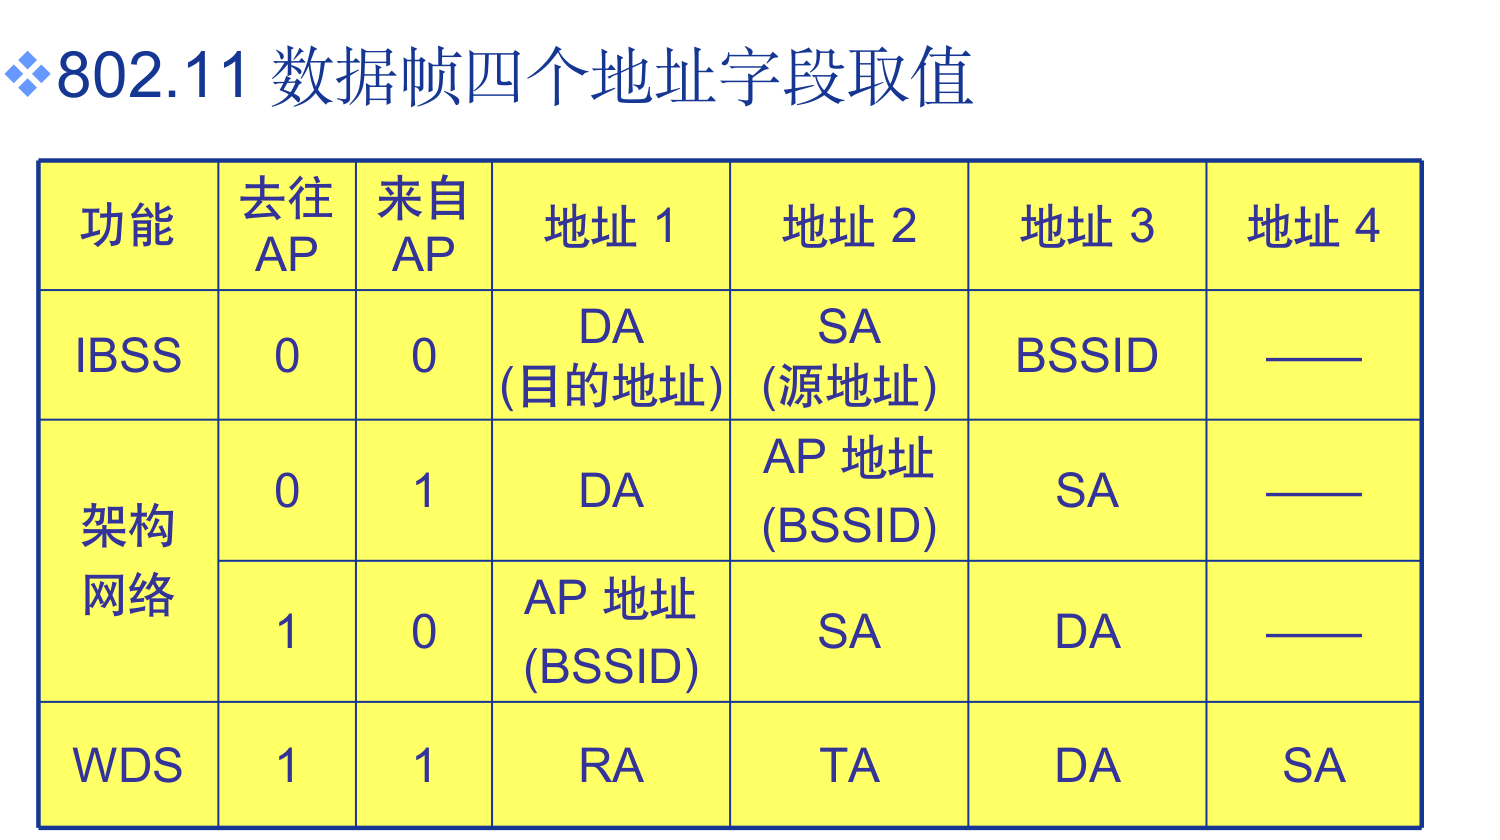
\includegraphics[width=.9\textwidth]{ch07-wifi-addresses.png}\caption{课件列出的四地址取值表。先读“去往AP/来自AP”两位，再按表确定地址1--4；WDS 行使用四个地址。来源：\texttt{Chapter7-无线与移动网络.pdf}，PDF阅读器第32页（显示页32），局部截取。}\label{fig:ch07-wifi-addresses}\end{figure}

\textbf{课件两页的表述不一致：} 第30页文字称地址4用于 ad hoc 或无线桥接；第32页表格则将 IBSS（自组网，去往/来自 AP 均为0）列为地址4空缺，只在 WDS（两位均为1）列出地址4。上述规则按课件第32页的完整取值表整理；复习时应注意第30页这句与表格之间的差异。
\annotationarea[4]
\small 来源：课件PDF阅读器第29--33页（显示页29--33）；参考教材第3章§3.6.3，PDF第108--109页（印刷第97--98页）。课件第30页关于地址4的描述与第32页取值表不一致，已在正文标明。\normalsize

\subsection{同子网移动、速率适应与节电}
如果主机在同一个互联网协议（IP，Internet Protocol）子网内从一个 AP 移动到另一个 AP，IP 地址可以保持不变。交换机通过主机发出的帧学习“该主机媒体访问控制（MAC，Medium Access Control）地址从哪个端口到达”，从而更新到达主机的端口信息。接入点改变是链路层位置变化，不必然意味着网络层 IP 地址改变。

无线信道质量变化时，设备还可以做\textbf{速率适应}：远离基站时 SNR 下降、BER 上升；当误码过高，就切换到较低速率的物理层方案，使传输更可靠。无线设备会在吞吐率与误码风险之间作选择。

\textbf{功率管理}用于节约电池。Wi-Fi 主机可通知 AP 自己进入休眠，AP 暂不向它发送帧并缓存下行数据；主机在下一个信标之前醒来。信标中的待发列表若显示 AP 有缓存帧，主机保持唤醒并接收；若无待发帧则继续休眠。

\subsection{蓝牙个人区域网络}
课件用蓝牙说明短距离无线个人区域网（PAN，Personal Area Network）。蓝牙覆盖范围通常小于10米，用于替代鼠标、键盘、耳机等设备的短连接；课件所列传统蓝牙使用2.4--2.5 GHz ISM（Industrial, Scientific and Medical，工业、科学和医疗）频段，速率最高约3 Mb/s。它可在没有固定基础设施时组织成微微网（piconet）：一个主控设备轮询客户端，为客户端传输请求分配机会。课件还介绍每个时隙约625微秒，并按已知伪随机次序在79个频率信道间跳频；停泊（parked）状态让暂不活动的设备休眠以节电。

\annotationarea[4]
\small 来源：课件PDF阅读器第34--38页（显示页34--38）；参考教材第3章§3.6.3，PDF第104--105页（印刷第93--94页）核对BSS与自组网络；教材第2章§2.2.1，PDF第54--55页（印刷第43--44页）核对无线介质。速率适应、节电和蓝牙时隙等按课件展开。\normalsize

\section{移动通信网络体系结构}
\subsection{蜂窝网络的基本组成}
蜂窝网络把覆盖区域划分成若干小区（cell），每个小区由基站服务。移动设备通过\textbf{空中接口}（air interface）与基站通信；该接口包含物理层和数据链路层协议。基站与 Wi-Fi AP 类似，都连接终端和更大网络，但蜂窝基站还要管理移动设备和无线资源，并与邻近基站协调切换。\textbf{移动交换中心}（MSC，Mobile Switching Center）连接若干小区与有线电话网，负责呼叫建立和移动性处理。

移动设备到基站的无线频谱要由多个终端共享。课件列出两种基本办法：\textbf{FDMA}（Frequency Division Multiple Access，频分多址）与\textbf{TDMA}（Time Division Multiple Access，时分多址）结合使用时，先把频谱分成频率信道，再把每个信道分成时间时隙；\textbf{CDMA}（Code Division Multiple Access，码分多址）允许多个发送者用不同码区分信号。它们分别从频率/时间资源和编码资源角度共享无线链路。

\subsection{2G、3G 与 4G LTE 的网络结构}
课件用几代蜂窝网络展示语音与数据网络逐步融合的过程：
\begin{itemize}[nosep]
  \item \textbf{2G 语音网络：}基站收发台 BTS（Base Transceiver Station）处理无线收发，基站控制器 BSC（Base Station Controller）管理一组基站；BTS 与 BSC 在课件中合称基站系统 BSS（Base Station System，此处不是 Wi-Fi 的 Basic Service Set）。MSC 连接电话网并进行呼叫交换；网关 MSC（Gateway MSC）是蜂窝网与公共交换电话网 PSTN（Public Switched Telephone Network）之间的入口/出口。
  \item \textbf{3G 语音与数据网络：}语音仍由原有 MSC/电话网承载；数据侧增加无线网络控制器 RNC（Radio Network Controller）、通用分组无线业务 GPRS（General Packet Radio Service）的服务支持节点 SGSN（Serving GPRS Support Node）和网关支持节点 GGSN（Gateway GPRS Support Node），通过 GGSN 接入公共互联网。课件重点指出数据网络与既有语音核心网并行运行。
  \item \textbf{4G LTE：}LTE（Long-Term Evolution）采用全 IP 核心网 EPC（Evolved Packet Core），语音和数据都进入 IP 核心网再到网关。终端 UE（User Equipment）通过演进型基站 eNode-B（evolved Node B）接入。移动管理实体 MME（Mobility Management Entity）主要处理控制面认证、移动管理和通道设置；归属用户服务器 HSS（Home Subscriber Server）保存用户/订阅信息；服务网关 S-GW（Serving Gateway）和分组数据网络网关 P-GW（Packet Data Network Gateway）位于数据转发路径上，P-GW 连接外部 IP 网络并可提供网络地址转换（NAT，Network Address Translation）。
\end{itemize}

\begin{figure}[H]\centering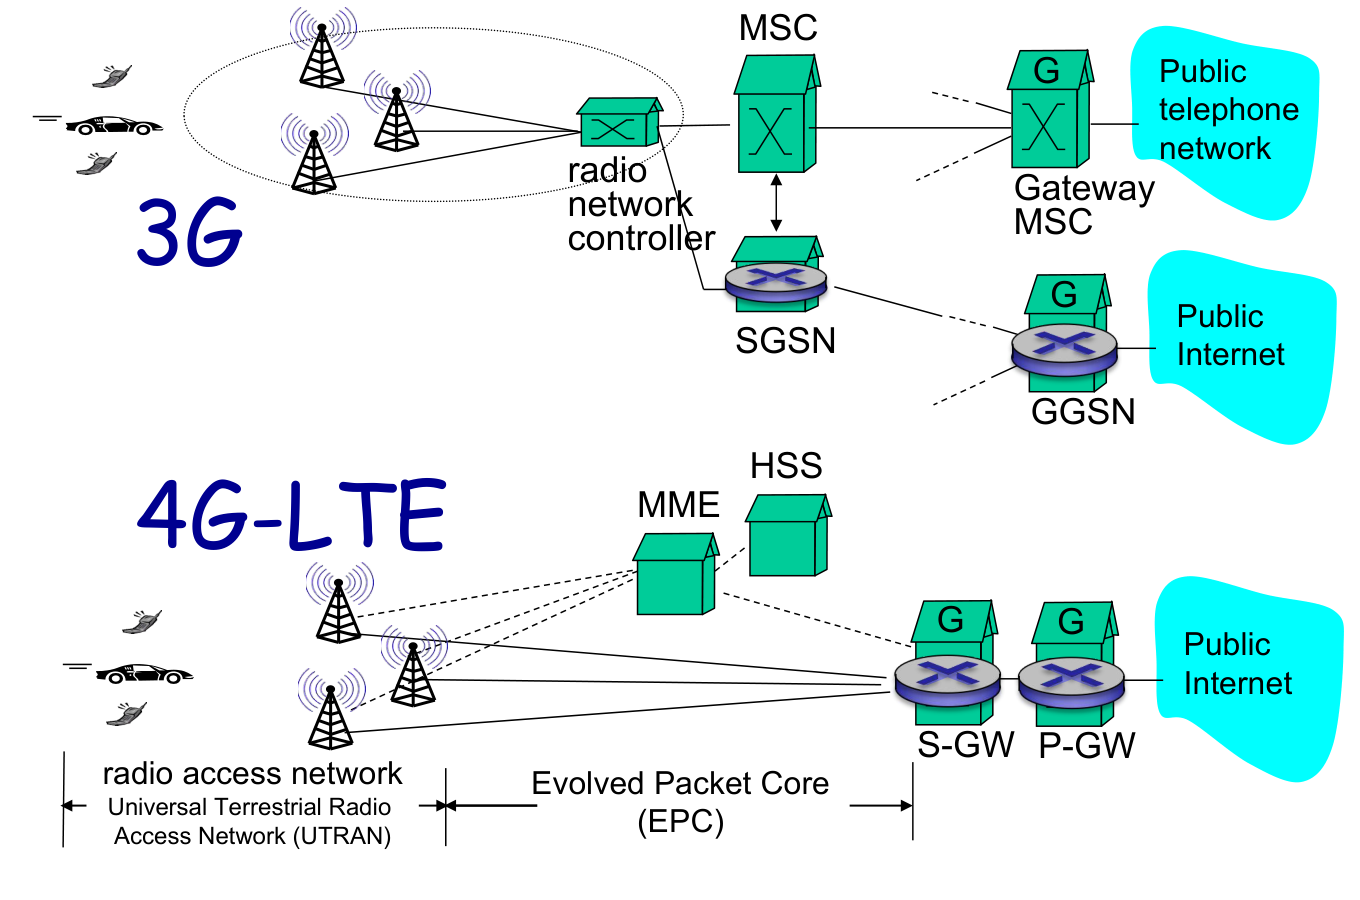
\includegraphics[width=.92\textwidth]{ch07-cellular-generations.png}\caption{课件中的 3G 与 4G LTE 网络结构对比：图中从无线接入网到核心网再到外部网络的连接关系不同。来源：\texttt{Chapter7-无线与移动网络.pdf}，PDF阅读器第45页（显示页45），局部截取。}\label{fig:ch07-cellular-generations}\end{figure}

\begin{figure}[H]\centering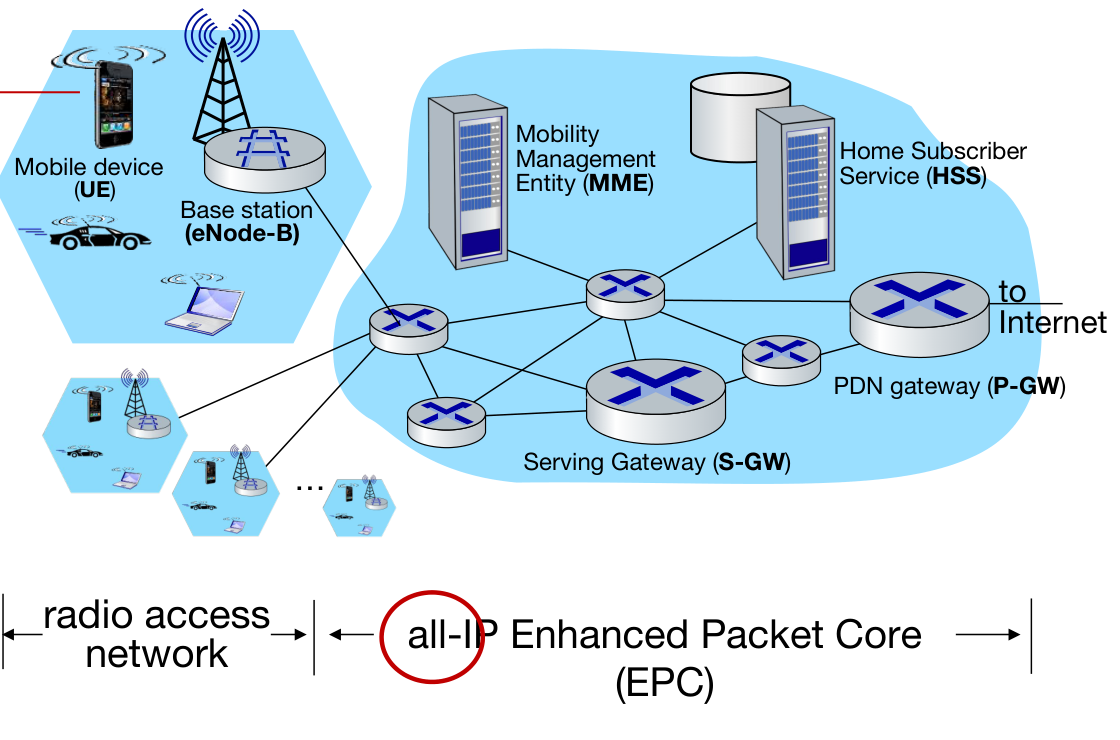
\includegraphics[width=.96\textwidth]{ch07-lte-architecture.png}\caption{LTE结构示意：左侧是 UE 与 eNode-B 无线接入，右侧 EPC 中的 MME/HSS 处理控制信息，S-GW/P-GW 转发用户数据。来源：\texttt{Chapter7-无线与移动网络.pdf}，PDF阅读器第49页（显示页49），局部截取。}\label{fig:ch07-lte-architecture}\end{figure}

课件列出的 LTE 部件职责可用“控制与数据分开”理解：MME 通过基站与移动设备通信，并向归属 HSS 查询鉴权、加密和服务信息；S-GW/P-GW 转发用户数据并建立隧道；基站管理本小区无线资源及终端。SIM（Subscriber Identity Module，用户识别模块）卡中保存 IMSI（International Mobile Subscriber Identity，国际移动用户识别码），用于标识用户及其归属网络，不等同于本次无线链路上的 MAC 地址或当前 IP 地址。课件第49、51页把 HSS 写作“Home Subscriber Service”，第90页写作“Home Subscriber Server”；本节采用课件第90页给出的 Server 写法。

\subsection{LTE 的数据面、协议栈与隧道}
在 LTE 首跳，课件从终端到基站列出分组数据汇聚（Packet Data Convergence）、无线链路控制 RLC（Radio Link Control）、媒体访问控制 MAC（Medium Access Control）和物理层等链路协议。分组数据汇聚层可做首部压缩与加密；RLC 可分片/重组并提供可靠数据传输；MAC 申请并使用无线时隙。下行采用频分复用 FDM（Frequency Division Multiplexing）并在频率信道内时分复用 TDM（Time Division Multiplexing），课件以 OFDM 说明子载波的正交性；课件图示每个活跃终端可分到两个或更多0.5 ms时隙、跨多个频率信道调度。调度算法由运营商实现，课件据此说明每终端可达到数百 Mb/s。

核心网广泛使用\textbf{隧道}：把终端的原始 IP 数据报放进 GTP-U（GPRS Tunneling Protocol User plane，用户面隧道协议）报文，再放入用户数据报协议（UDP，User Datagram Protocol）和外层 IP 数据报中，送到 S-GW；S-GW 解封装或重新封装后继续送往 P-GW。外层 IP 地址用于把隧道报文送到隧道另一端；内层 IP 数据报仍是终端与互联网服务器之间的原始数据。终端切换基站时，网络可更新隧道端点，而不要求每个外部通信对端都改写其目的地址。

\begin{figure}[H]\centering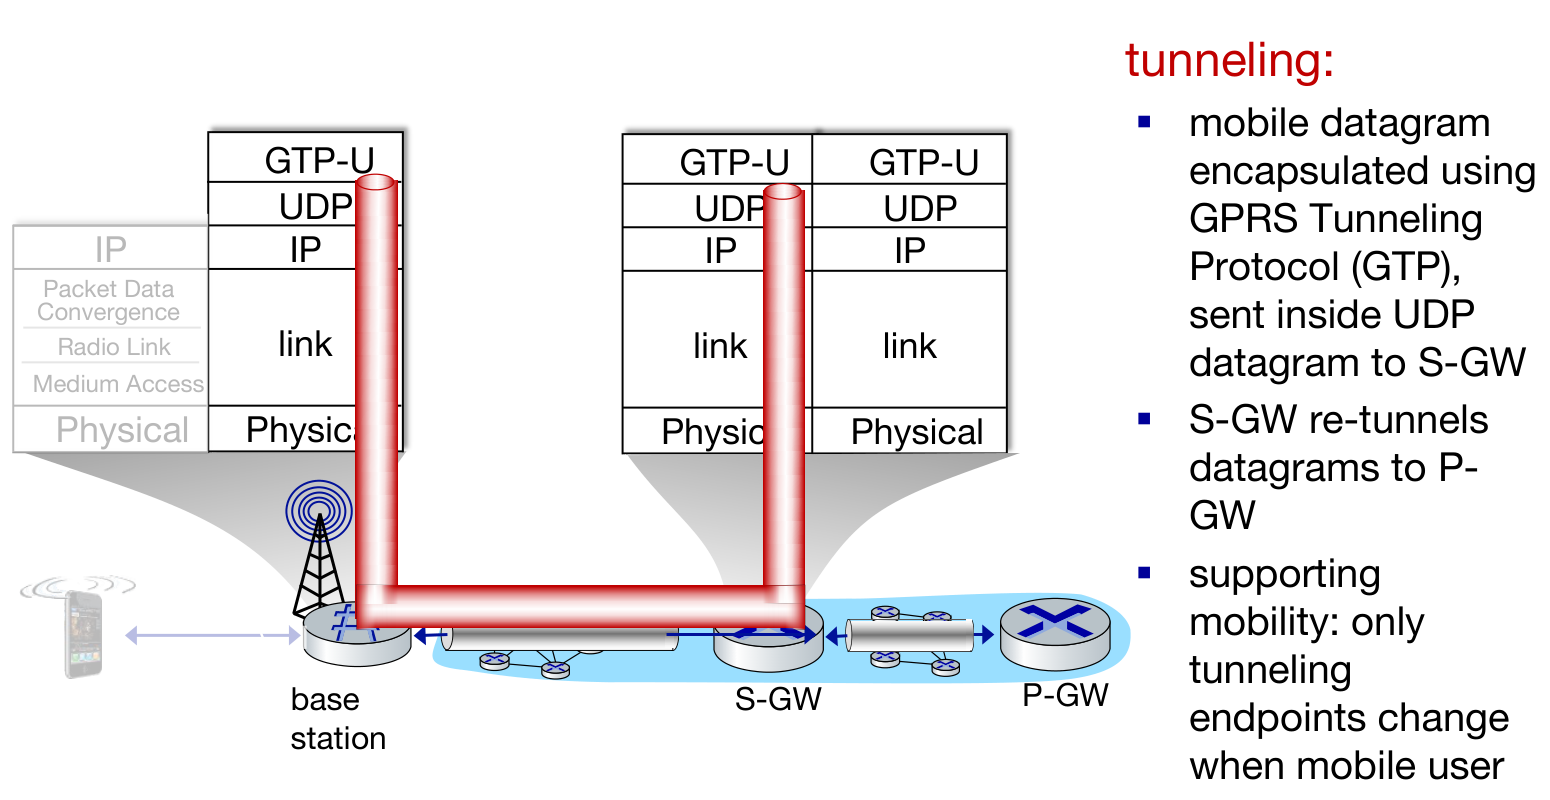
\includegraphics[width=.9\textwidth]{ch07-lte-tunnel-stack.png}\caption{LTE核心网隧道封装：红色路径表示终端数据经基站、S-GW到P-GW；右侧协议栈显示GTP-U/UDP/IP等外层封装。来源：\texttt{Chapter7-无线与移动网络.pdf}，PDF阅读器第57页（显示页57），局部截取。}\label{fig:ch07-lte-tunnel-stack}\end{figure}

移动设备与基站建立关联也有步骤：课件称基站每5 ms周期发送同步信号，设备先找到主同步信号，再找到该频率上的第二同步信号，读取带宽、网络配置和运营商信息；设备选择基站后仍要进行身份认证、状态配置及数据路径建立。休眠中的终端可以进入轻睡眠（课件举例为数百毫秒不活动后进入，并周期醒来检查下行帧）；无活动数秒后进入深睡眠，若休眠中移动到另一小区，醒来后需要重新建立关联。课件说明全球蜂窝网络通过运营商之间的互联点及公共互联网连接，归属 HSS 保存用户身份与服务信息；漫游时访问网络要能联系其归属网络。

\subsection{5G 课件概览}
课件以 5G NR（New Radio，新空口）说明后续发展：相对4G，课件列出的设计目标为峰值比特率提高10倍、时延降低10倍、流量容量提高100倍；频率范围 FR1（Frequency Range 1）约450 MHz--6 GHz、FR2（Frequency Range 2）约24--52 GHz。毫米波可支持更高数据率但覆盖距离较短，为此需要部署更密集的基站和更小的小区（课件称 pico-cell）。这些频段与目标倍数是课件中的技术概览，不是对每个实际部署的保证值。
\annotationarea[4]
\small 来源：课件PDF阅读器第40--61页（显示页40--61）；无线空口共享与无线介质可参考教材第2章§2.2.1，PDF第54--55页（印刷第43--44页）。教材未按课件展开2G/3G/4G/5G蜂窝核心网、LTE控制面和GTP隧道，本节相应机制以课件为依据。\normalsize

\section{网络移动管理基本原理}
\subsection{移动性的范围与位置管理}
从网络角度看，移动程度可以从低到高：设备完全不移动；设备在移动时关机，到新网络后再启动；设备在同一提供商网络内换接入点；设备在多个提供商网络间移动，同时保持正在进行的连接。课件重点讨论后两类：通信持续期间接入点或服务网络改变时，网络怎样知道设备当前位置并将数据送到那里。

一种办法是让互联网路由器通过常规路由信息广播移动节点的永久地址或编号所在位置，照普通前缀路由转发。课件认为这种办法理论上可行，但若为大量移动设备频繁发布主机级路由，会令全球路由表难以扩展。另一办法把功能放到网络边缘：设备或其归属网络登记当前接入位置，通信对端通过归属网络找到设备。

\textbf{归属网络}是用户订阅服务的运营商网络，保存用户身份、服务资料和当前所在位置；4G课件中这类资料由 HSS 保存。\textbf{访问网络}（visited network）是设备当前接入的其他运营商网络，双方通常需有漫游服务协议。在普通 ISP/Wi-Fi 接入中，往往没有统一的全球“归属网”登记机制，凭据可能是本地用户名、密码；因此不同 Wi-Fi 网络可能需要不同认证信息。

\subsection{间接路由与直接路由}
\textbf{间接路由}让通信对端始终向设备的永久地址发送。归属网络收到数据后查询设备最新登记的位置，再通过隧道把数据转发到访问网络；访问网络交付给设备。回复流量可以先回归属网络，也可以从访问网络直接发给通信对端。这样对端不必知道设备在哪个访问网络，移动到另一访问网后只需重新登记；代价是可能绕远，若通信双方本就在同一访问网络而数据仍经归属网，就形成“三角路由”式的低效路径。

\textbf{直接路由}由通信对端先向归属网络查询当前位置，再直接向访问网络发送数据。它能减少绕路，但对端必须得到并更新设备的访问地址；设备再次移动时，位置变化处理更复杂，通信也不再对端完全透明。

\begin{figure}[H]\centering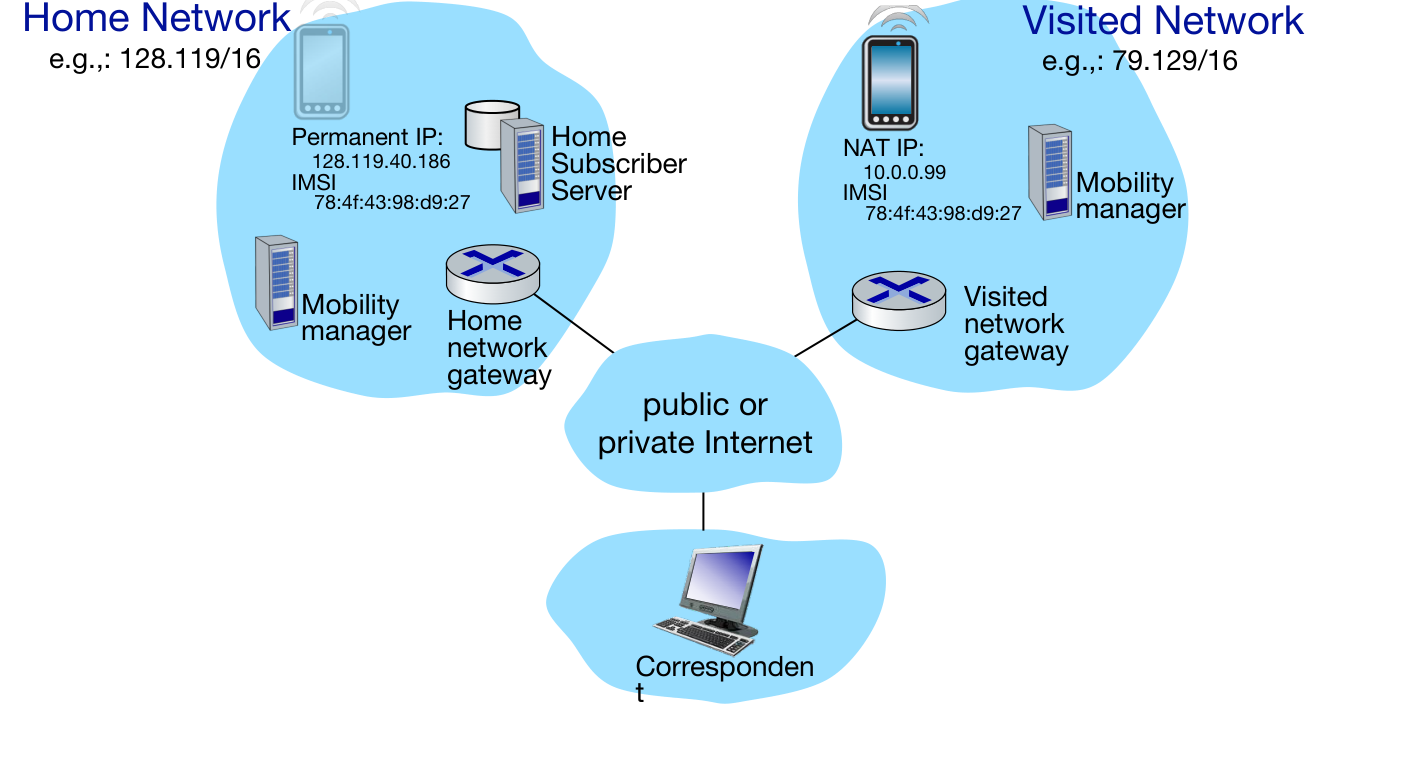
\includegraphics[width=.95\textwidth]{ch07-indirect-routing.png}\caption{归属网与访问网的拓扑关系：左右蓝色区域分别表示归属网络和访问网络，中间区域表示公共或专用互联网，下方区域表示通信对端；图中网关连线表示这些网络之间的互联关系。来源：\texttt{Chapter7-无线与移动网络.pdf}，PDF阅读器第69页（显示页69），局部截取。}\label{fig:ch07-indirect-routing}\end{figure}

在课件的 4G/5G 场景，移动设备先与访问网络基站关联并用 IMSI 表明归属；MME 与归属 HSS 配置控制面状态，确认设备当前位于访问网；MME 再设置用户面隧道，从归属 P-GW 经访问网转发到移动设备。设备换基站时，网络发起切换并更新转发端点。这样控制面负责“身份、位置与通道配置”，数据面负责“实际分组转发”。
\annotationarea[4]
\small 来源：课件PDF阅读器第63--74页（显示页63--74），第89--93页（显示页89--93）；移动IP与间接路由参考教材第4章§4.6，PDF第223--225页（印刷第212--214页）。教材未覆盖课件的蜂窝 HSS/MME 控制面分工。\normalsize

\section{移动 IP}
\subsection{永久地址、转交地址与代理}
移动 IP 是课件介绍的网络层移动性机制：移动节点离开归属网络后仍保留\textbf{永久地址}（归属地址），让通信对端继续使用同一目的地址；网络另为它登记当前访问位置，并把到达永久地址的数据转发过去。移动 IP 课件描述的是经归属网络间接转发的模型。

关键实体有：\textbf{移动节点}（mobile node），持有永久地址的移动设备；\textbf{归属代理}（home agent），位于归属网络，记录永久地址到当前转交地址的对应关系并截获发往移动节点的分组；\textbf{外地代理}（foreign agent），位于访问网络，协助移动节点登记和接收转发分组；\textbf{转交地址}（care-of address, COA），表示节点在访问网络中的当前可达位置。永久地址保持不变，转交地址随访问网络变化。

\subsection{代理发现、注册与数据转发}
课件把移动 IP 归纳为三项机制：间接路由、代理发现、向归属代理注册。代理发现时，归属代理或外地代理广播 ICMP（Internet Control Message Protocol，网际控制报文协议）代理通告；课件图中以 ICMP Router Advertisement（类型字段为9）及移动代理扩展表示，扩展携带代理类型标志、注册期限和一个或多个 COA。移动节点据此判断当前网络是否为归属网，或发现外地代理提供的转交地址。

移动节点获得 COA 后发起注册：注册请求携带移动节点永久地址、归属代理地址、COA、请求有效期和标识；外地代理把请求转给归属代理。归属代理接受后返回注册应答，外地代理再转给移动节点。归属代理据此保存绑定，知道“发往永久地址的分组应经隧道送到哪个 COA”。\textbf{参考书补充：}移动节点回到归属网络时，可注销或更新该绑定，恢复本地直接交付。

数据到达时，通信对端仍把永久地址作为目的 IP。归属代理收到后，在原数据报外再加一个新的 IP 首部，使外层目的地址为 COA；这是\textbf{隧道封装}，也叫“分组中的分组”。外地代理接收外层分组、移除外层首部，取出原始数据报后交给移动节点。外发数据则可由移动节点直接经过访问网络发往通信对端，因此去程经过归属代理、回程可能不经过它。

\begin{figure}[H]\centering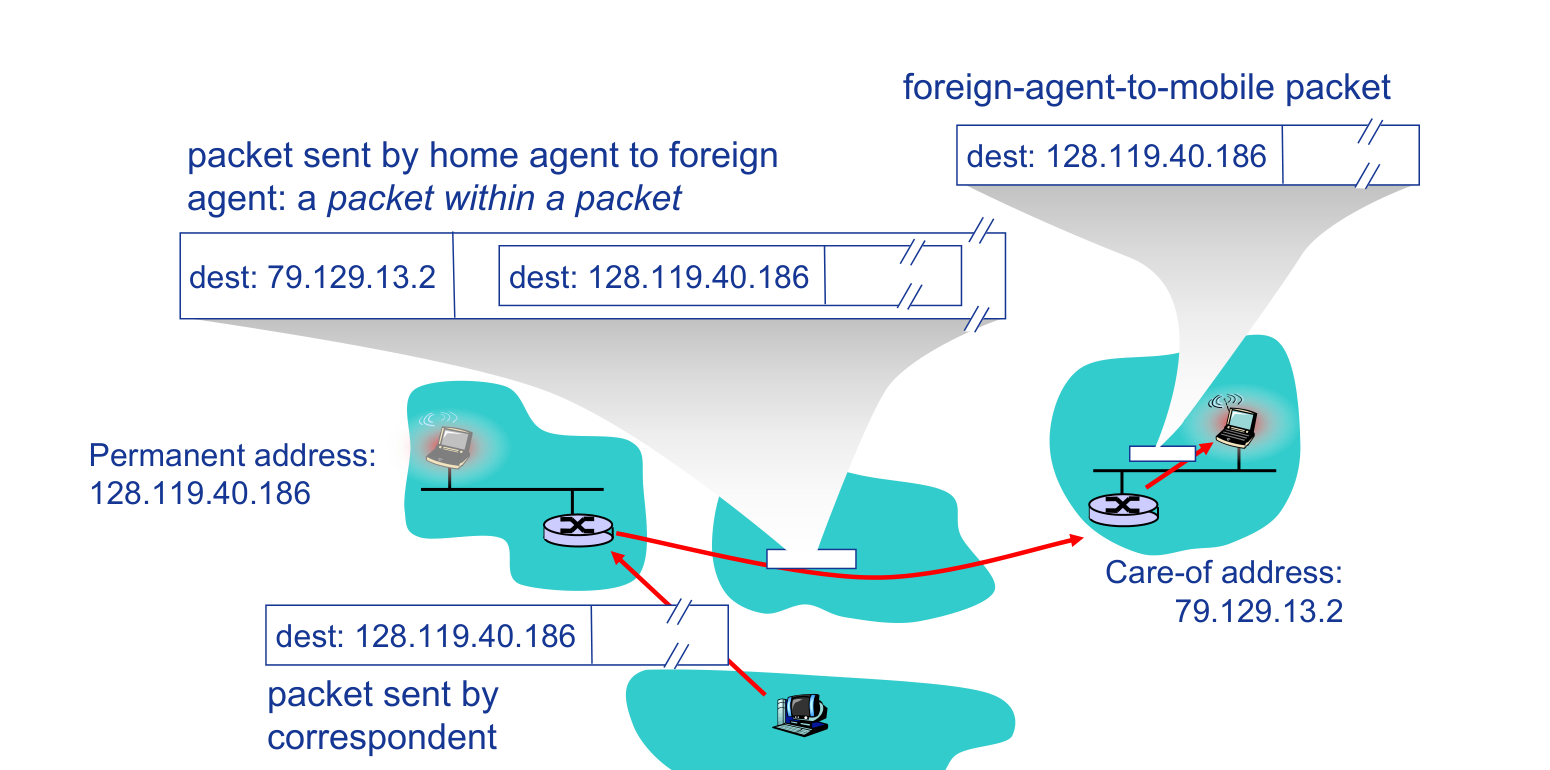
\includegraphics[width=.94\textwidth]{ch07-mobileip-tunnel.png}\caption{移动 IP 间接转发：原始分组目的地址是永久地址；归属代理封装后以 COA 为外层目的地址，经隧道送至外地代理；解封装后仍交给永久地址对应的移动节点。来源：\texttt{Chapter7-无线与移动网络.pdf}，PDF阅读器第78页（显示页78），局部截取。}\label{fig:ch07-mobileip-tunnel}\end{figure}

\textbf{课件注册示例（PDF第80页）：}访问网络为 79.129.13/24；移动节点永久地址为 128.119.40.186，外地代理提供 COA 79.129.13.2，归属代理地址为 128.119.40.7。节点发现代理后，请求把 79.129.13.2 登记到 128.119.40.7；请求示例中的 Lifetime（有效期）为9999，标识号为714；返回应答使用相同标识号，示例同意的有效期为4999。归属代理收到并接受登记后，便可把送往 128.119.40.186 的分组经隧道发往 79.129.13.2。课件给出的有效期数值是报文示例，重点是请求与应答的往返登记关系。

\begin{figure}[H]\centering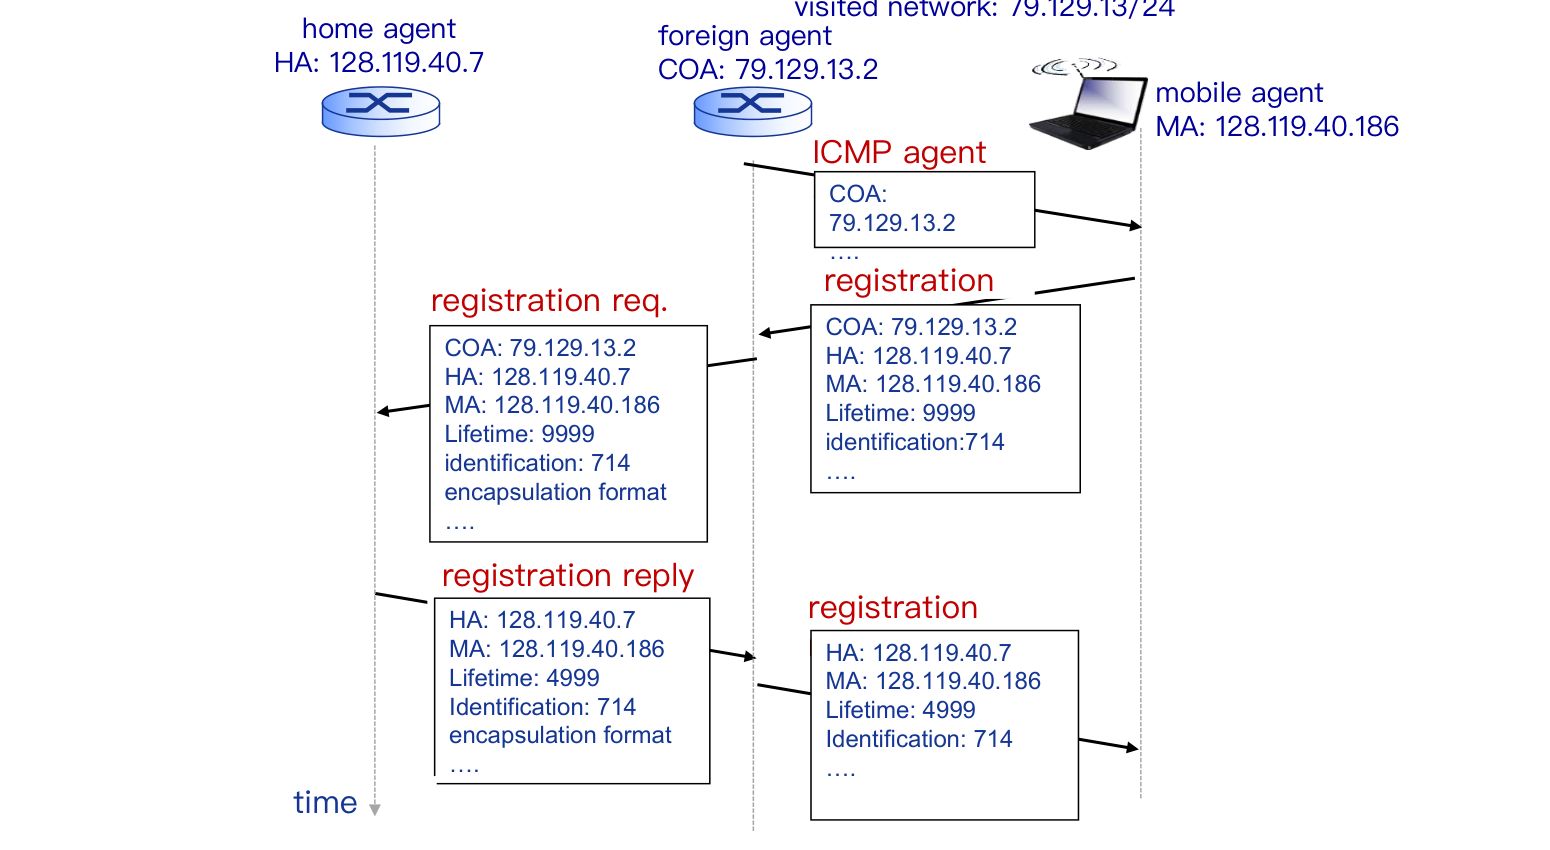
\includegraphics[width=.91\textwidth]{ch07-mobileip-registration.png}\caption{移动 IP 注册时间线：代理先通告 COA，移动节点请求登记到归属代理，注册应答沿外地代理返回；数值字段是课件中的示例。来源：\texttt{Chapter7-无线与移动网络.pdf}，PDF阅读器第80页（显示页80），局部截取。}\label{fig:ch07-mobileip-registration}\end{figure}

\textbf{间接与直接路由比较。} 间接路由把位置管理集中在归属代理，通信对端仍只需知道永久地址，移动后便于维持连接，但可能绕路。直接路由要求通信对端查询移动节点的访问地址并直接发送，较少绕路，却要把位置变化告知通信对端。课件指出早期移动 IP 采用隧道间接路由；教材也强调归属地址不变、COA动态变化及归属代理到外地网络的隧道。

\textbf{教材补充练习（移动 IP，参考书PDF第224--225页）：}
\begin{enumerate}[nosep]
  \item 判断“移动节点到达新网络后，把新的可达信息通知外地代理”是否正确。\textbf{解：}不正确。移动节点把 COA 等登记信息交给外地代理协助转发；真正需要获知该移动节点新位置并建立转发绑定的是归属代理。归属代理随后把分组隧道到该 COA。
  \item 移动 IP 的归属地址和转交地址如何变化？\textbf{解：}归属地址对应归属网络，移动时保持不变；COA 标识访问网中的当前可达位置，换访问网络时会改变，返回归属网时可注销。
  \item 主机 160.80.40.20/16 移动到不属于 160.80/16 的网络，若没有移动 IP，能否收发？\textbf{解：}它可把原永久地址作为源地址发出分组，访问网络的默认路由仍可能转发出站流量；但发往 160.80.40.20 的入站分组会被路由到其归属前缀，而不会自然到达新网络。因此在课件所问的直接收发中，能直接发送、不能直接接收（对应教材选项D）。
\end{enumerate}
\annotationarea[4]
\small 来源：课件PDF阅读器第76--80页（显示页76--80）；参考教材第4章§4.6.1--§4.6.4，PDF第223--225页（印刷第212--214页）。课件第76页列RFC 5944，第77页列RFC 3344，引用版本不同；本文按课件给出的移动IP基本模型整理，不据此扩展协议版本差异。\normalsize

\section{移动通信网络的移动管理}
\subsection{GSM 归属/访问位置登记与寻呼路由}
课件用 GSM（Global System for Mobile Communications，全球移动通信系统）说明蜂窝语音网络中的位置登记。\textbf{归属位置寄存器} HLR（Home Location Register）位于归属网络，保存用户永久电话号码、服务资料及当前所在网络等信息；\textbf{访问位置寄存器} VLR（Visitor Location Register）为当前访问网络中的用户保存临时登记信息。访问网络可以就是归属网络。

当呼叫者拨打移动用户号码时，呼叫先到归属网络 MSC；归属 MSC 查询 HLR，得到该用户当前访问网络的可路由号码，再建立通往访问网络 MSC 的第二段呼叫；访问 MSC 最后通过相应基站连接移动用户。关键点是电话网络先联系用户归属地，再由归属位置记录找到当前访问网络。

\subsection{GSM 切换}
\textbf{切换}是通信中的移动设备从旧基站转到新基站，同时尽量保持当前通话或连接。课件列出的触发理由包括：新基站信号更强、持续连接更可靠/节省电池，或网络需要负载均衡。GSM 规范描述如何进行切换，但不强制网络必须按哪一种策略决定何时切换。

同一 MSC 管理范围内的切换按课件时序可读成八步：
\begin{enumerate}[nosep]
  \item 旧基站向 MSC 报告即将切换，并提供一个或多个候选新基站。
  \item MSC 为到新基站的路径分配资源。
  \item 新基站为移动设备预留无线信道。
  \item 新基站通知 MSC 和旧基站“新信道准备好”。
  \item 旧基站通知移动设备切换到新基站。
  \item 移动设备和新基站激活新信道。
  \item 移动设备通过新基站向 MSC 报告切换完成，MSC 改走新路径。
  \item 释放 MSC 与旧基站之间不再需要的资源。
\end{enumerate}

\begin{figure}[H]\centering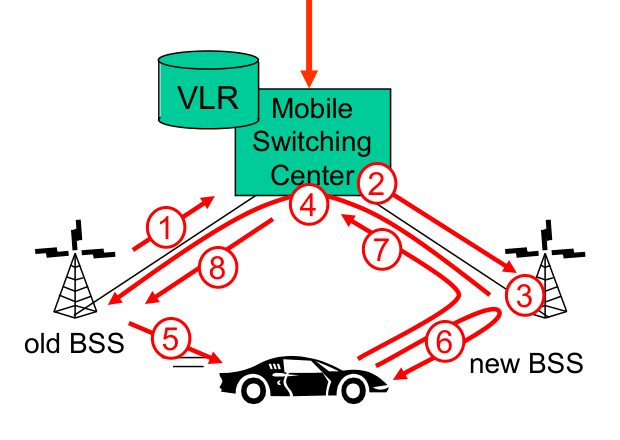
\includegraphics[width=.9\textwidth]{ch07-gsm-handoff.png}\caption{同一 MSC 内 GSM 切换的八个事件：旧基站启动流程，新基站先准备信道，移动设备接入新基站后 MSC 改路并释放旧资源。红色数字表示事件顺序。来源：\texttt{Chapter7-无线与移动网络.pdf}，PDF阅读器第85页（显示页85），局部截取。}\label{fig:ch07-gsm-handoff}\end{figure}

若设备在通话中切换到另一个 MSC，课件把最初接入的 MSC 称为\textbf{锚 MSC}（anchor MSC）。通话仍经锚 MSC；每次移动到新 MSC 时，可在原转发链上增加新的 MSC。这样可以继续保持通话，但链路可能越来越长；网络可选做路径最小化以缩短转发链。

\subsection{4G LTE 基站切换}
LTE 中 MME 管理移动状态，S-GW/P-GW 处于数据路径上。课件把基站间切换分为控制信令和转发调整两部分。以下按 PDF 第92--93页逐事件解释：
\begin{enumerate}[nosep]
  \item 源基站选择目标基站，发送 Handover Request（切换请求）。
  \item 目标基站预分配无线时隙/资源，并向源基站发送 Handover Request Acknowledgment（切换请求确认），其中包含供移动设备使用的信息。
  \item 源基站把目标基站信息通知移动设备；移动设备开始通过目标基站通信。
  \item 源基站停止向移动设备直接发送数据，而把暂时到达的分组转发给目标基站，由目标基站通过无线链路交付。
  \item 目标基站告知 MME 自己成为该移动设备的新基站；MME 指示 S-GW 更新隧道端点。
  \item 目标基站向源基站确认切换结束，源基站释放旧资源。
  \item 移动设备数据改走从目标基站到 S-GW 的新隧道。
\end{enumerate}

\begin{figure}[H]\centering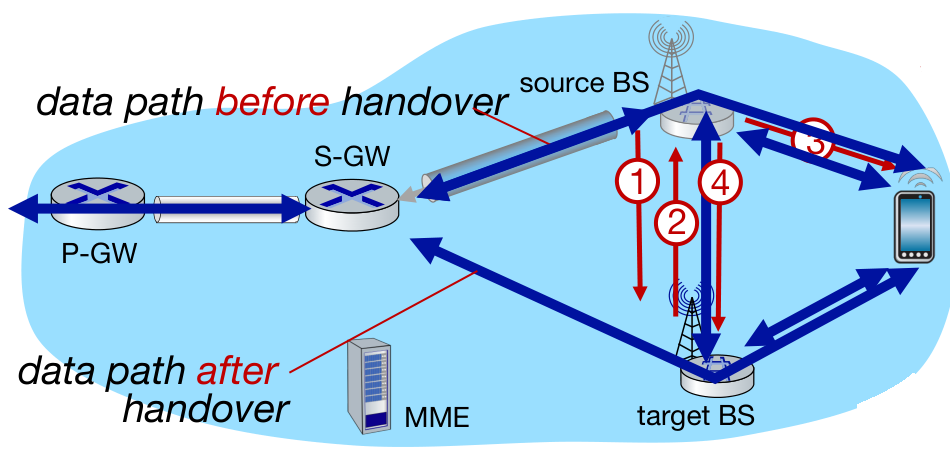
\includegraphics[width=.96\textwidth]{ch07-lte-handover-1.png}\caption{LTE 基站切换前半段：源基站请求目标基站准备，目标分配无线资源，移动设备改由目标基站接入，源基站临时转发尚未送达的分组。来源：\texttt{Chapter7-无线与移动网络.pdf}，PDF阅读器第92页（显示页92），局部截取。}\label{fig:ch07-lte-handover-1}\end{figure}
\begin{figure}[H]\centering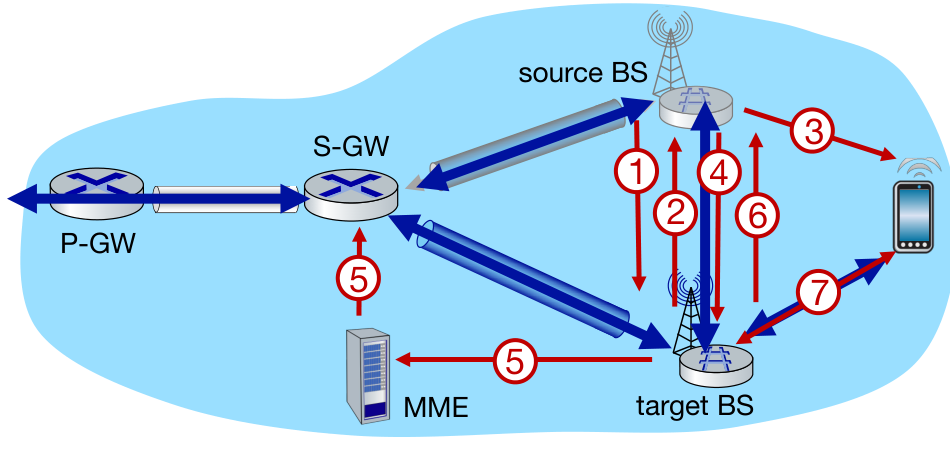
\includegraphics[width=.94\textwidth]{ch07-lte-handover-2.png}\caption{LTE 基站切换后半段：目标基站更新 MME，MME 改设 S-GW 隧道端点，确认后释放源基站资源，数据最终经目标基站的新隧道转发。来源：\texttt{Chapter7-无线与移动网络.pdf}，PDF阅读器第93页（显示页93），局部截取。}\label{fig:ch07-lte-handover-2}\end{figure}

\subsection{蜂窝移动管理与移动 IP 的联系}
课件用比较表把 GSM 组件与移动 IP 概念对应：归属系统类似归属网络；归属 MSC/HLR 的职责与归属代理部分相似；访问 MSC/VLR 的职责与外地代理部分相似；GSM 的移动台漫游号码 MSRN（Mobile Station Roaming Number）承担访问路径的可路由地址作用，移动 IP 中相应概念是 COA。二者都需要归属侧位置记录，并把发往永久身份/地址的数据转到当前访问位置；但一个是蜂窝电话呼叫架构，一个是 IP 数据报转发架构，组件名称和协议流程不能直接等同。

\annotationarea[4]
\small 来源：课件PDF阅读器第82--93页（显示页82--93）；移动 IP 与 GSM 对照参考教材第4章§4.6，PDF第223--225页（印刷第212--214页）。GSM、LTE 的 HLR/VLR、MSC、MME 与切换细节以课件为依据。\normalsize

\section{无线与移动对高层协议的影响}
无线链路和移动接入不会改变网络层的尽力而为服务模型：传输控制协议（TCP，Transmission Control Protocol）、用户数据报协议（UDP，User Datagram Protocol）和 IP 仍可运行在无线网络上。变化主要出现在性能方面：无线误码会使链路层丢弃数据或通过重传带来额外时延；切换过程中也可能短暂丢包或延迟。TCP 看到丢包时通常把它当成拥塞信号，缩小拥塞窗口；但无线链路的位错误或切换丢包未必来自网络拥塞，因此可能不必要地降低吞吐量。实时业务会感受到额外时延，而无线频谱/带宽本身也是稀缺资源，需要合理共享。

\textbf{复习时抓住因果链：} 无线误码、隐藏终端和切换都可能引起丢包/等待；链路层的确认、重传和调度可改善链路可靠性，但会增加时延；传输层和应用层观察到的是最终时延与丢失，未必知道其来自拥塞、无线误码还是移动切换。
\annotationarea[4]
\small 来源：课件PDF阅读器第95页（显示页95）。本节具体性能影响依课件总结；参考教材相应章节用于核对无线链路、可靠传输与TCP拥塞反应，不将教材未在此处展开的机制写成课件结论。\normalsize


\end{document}

